\chapter*{}

\begin{vplace}[0.7]
Fiódor Dostoiévski, me responda de uma vez: por que a vida e a história não desmentem Franz Kafka, quando ele sentencia que há esperança, mas não para nós?
\end{vplace}
\thispagestyle{empty}

\chapter*{De futebol e letras}
\addcontentsline{toc}{chapter}{[Prefácio] De futebol e letras, por \emph{Fábio Altman}}

\begin{flushright}
\emph{Fábio Altman}\footnote{{Fábio Altman} é redator"-chefe da revista \emph{Veja}.}
\end{flushright}

Nenhuma Copa do Mundo teria graça se fosse apenas futebol, ainda que
pudéssemos grudar nas retinas apenas os lances geniais de Pelé, Cruyff e
Maradona. Aquele quase"-gol contra o Uruguai em 1970, a
\emph{Blietzkrieg} holandesa de 1974 e a milagrosa arrancada do
\emph{pibe} contra a Inglaterra em 1986. Pensando nisso, na riqueza do
que seria o torneio de 2018 na Rússia, para muito além do gramado,
passei um bom tempo quebrando a cabeça de modo a imaginar uma edição
especial de \emph{Veja} que desse conta de tanto passado e tanto
presente. Das páginas do extraordinário \emph{Uma história cultural da
Rússia}, do historiador inglês Orlando Figes, extraí uma frase que me
guiaria semanas a fio, o livro pousado ao lado da cama, ora
insistentemente aberto, ora fechado. Para Figes, o país ``convida o
historiador a sondar debaixo da superfície de aparência artística. Nos
últimos duzentos anos, as artes da Rússia serviram de arena para o
debate político, filosófico e religioso, na ausência do parlamento e da
imprensa livre''\footnote{Orlando Figes, \emph{Uma história cultural da
  Rússia}. Tradução de Maria Beatriz Medina. Rio de Janeiro: Record,
  2017, p. 21.}. Parecia evidente que o esporte, ao desembarcar na
Rússia, também não poderia ficar na superfície. Uma ideia, que nasceu
pequena, cresceu, mas morreu dado o absurdo de sua concepção, e que
renasceria na marra, foi a de associar os grandes nomes da seleção
brasileira -- Tite, Neymar e Gabriel Jesus -- a personagens da
literatura russa. Não sabia por onde começar, a não ser pela escolha
óbvia de \emph{Guerra e paz} como carbono do brasileiro Neymar no
francês \versal{PSG}, como se o craque fosse um Pierre Bezukhov qualquer. Não
poderia dar certo -- uma saída aparentemente imaginativa, a das
comparações, exigiria conhecimento minucioso das letras russas, e não as
relações superficiais e sem charme que eu mesmo conseguiria inventar.

Como quase todo jornalista sabe muito pouco de muita coisa, mas sabe
achar quem sabe, salvou"-me um amigo, o editor e escritor Tiago Ferro,
autor do obrigatório e bonito \emph{O pai da menina morta}\footnote{Tiago Ferro, \emph{O pai da menina morta.} São Paulo: Todavia, 2018.}.
Consultado, Tiago não demorou cinco minutos para me indicar Flávio
Ricardo Vassoler, a quem não conhecia pessoalmente, mas que colaborara
com a revista eletrônica \emph{Peixe elétrico}. Encontrei Flávio Ricardo
no \emph{Facebook} (ele estava em viagem de férias e trabalho na
Croácia). Marquei um almoço para quando ele retornasse, dali a duas
semanas. Antes mesmo da sobremesa, aquele mais novo velho amigo de
infância sacou de uma mente sempre elétrica os pares de Tite, Neymar e
Gabriel Jesus e ofereceu um cardápio de tradutores e professores que
poderiam me acompanhar na empreitada. Tite seria o Tarás Bulba de
Nikolai Gógol. Neymar, o Nikolai Stavróguin de \emph{Os demônios}, de
Fiódor Dostoiévski. Gabriel Jesus era a cara de Ivan Ilitch, o jurista
de \emph{A morte de Ivan Ilitch}, de Liev Tolstói. E assim foi. O time
estava completo, e \emph{Veja} chegou às bancas, no início de junho, com
essa escalação. 
Flávio Ricardo, que comprou o plano com o entusiasmo de
uma criança presenteada com a primeira bola de futebol, não parou mais,
até chegar às páginas deste \emph{Diário de um escritor na Rússia}.

Na preparação da edição de \emph{Veja} destinada a apresentar a Copa do
Mundo, outro capítulo foi a organização de um campeonato imaginário com
dezesseis grandes escritores russos. Eles foram divididos em duas chaves
de oito competidores. A convite de \emph{Veja}, um elenco de nove
especialistas no tema -- tradutores, professores e jornalistas --
escolheu o vencedor de cada partida, rodada a rodada, até a finalíssima.
Flávio Ricardo era um dos jurados. Inconsolado, quase se revoltou com a
vitória de Púchkin, o grande campeão, contra Tolstói. Para ele, foi um
erro crasso ter deixado Púchkin vencer Dostoiévski numa das semifinais.
Mas não houve \versal{VAR} que mudasse os resultados, porque regras são regras.
Até hoje, rindo, mas seriamente, Flávio Ricardo lamenta a derrota de
Dostoiévski, o maior de todos. ``Esse título tinha de ser de Fiódor'',
ele resume. Contaminado pelo vírus do que \emph{Veja} desenhava, o
``professor'', como ficou conhecido entre os jornalistas que cobririam a
Copa, e a quem convidei a dar uma palestra sobre história e literatura
dias antes do embarque, queria muito mais -- o pouco que lhe fora
oferecido não cabia em sua criatividade e inteligência, em seu domínio
de português e russo, em suas vastas ambições.

Foi dele a sacada, imediatamente aceita, de refazer o \emph{Diário de um
escritor} que Dostoiévski escrevera na década de 1870. O plano era
atravessar a Rússia ocidental e diariamente enviar
crônicas/ficções/ensaios que fizessem uma linha de passe com a
literatura, a história, o ontem e o hoje, com pinceladas de futebol --
pedi a ele que não tratasse muito do que haveria dentro de campo e que
se apegasse a seu caminho muito original. Flávio Ricardo impôs a si
mesmo um ritmo homérico. Um texto por dia, sagradamente, enviados de dez
diferentes cidades russas, às vezes do interior de vagões de trens
noturnos, entre um ponto e outro. E todas as noites, de 15 de junho a 15
de julho de 2018, piscava em meu \emph{e"-mail}, infalível, com o rigor
de um comissário comunista, a mensagem de Flávio Ricardo com linhas
extraordinárias, elegantes, um tanto líricas, sempre precisas, misto de
reportagem e história, verdadeiras aulas. De \emph{Diário de um escritor
pela Rússia de Dostoiévski e Tolstói, Maiakóvski e Stálin, Gagárin e
Putin}, o relato número 1, assinado de Moscou, a \emph{Adeus às armas?},
o relato número 31, de São Petersburgo, o que os leitores do \emph{site}
de \emph{Veja} puderam acessar, enquanto a seleção ia mal das pernas e
Neymar cismava em rolar na relva, são pequenas obras"-primas, agora
reunidas em livro. É coisa de Pelé, Cruyff e Maradona -- é a
comprovação, tudo somado, de que não é só futebol. Prestemos atenção ao
trabalho de Flávio Ricardo Vassoler.

%\clearpage{\pagestyle{empty}\cleardoublepage}
%\movetooddpage

%\pagebreak
\clearpage
\thispagestyle{empty}

%\makeatletter\@openrightfalse
\movetoevenpage
\begin{absolutelynopagebreak}
\begin{vplace}
\begin{figure}[H]
\begin{adjustwidth}{-1.8cm}{}
  %\centering
  \vspace{2.7cm}
  %\hspace{-0.5cm}
  \includegraphics[width=130mm]{./imgs/moscou2.jpg}  
  %\hfill
\end{adjustwidth}
  \caption{Estátua equestre do general soviético Georgui Júkov (1896-1974), herói da resistência à invasão nazista, em frente ao Museu de História Russa, nas imediações da Praça Vermelha, em Moscou}

\thispagestyle{empty}

\end{figure}
\end{vplace}

\end{absolutelynopagebreak}

\movetooddpage
\addcontentsline{toc}{part}{Moscou [km 0]}
\part*{MOSCOU -- KM 0}


\movetooddpage
\chapter*{Diário de um escritor pela Rússia de Dostoiévski e Tolstói, Maiakóvski e Stálin, Gagárin e Putin}
\addcontentsline{toc}{chapter}{[15/06/18] Diário de um escritor pela Rússia de Dostoiévski e Tolstói, Maiakóvski e Stálin, Gagárin e Putin}
%\@openrighttrue\makeatother

\begin{flushright}
\emph{Moscou, 15 de junho de 2018}
\end{flushright}

Ao longo da década de 1870, o escritor russo Fiódor Dostoiévski compôs o
\emph{Diário de um escritor}, cujos textos de cunho literário e
filosófico, histórico e político contribuíram sobremaneira para
disseminar a obra do autor dos famosos cinco elefantes: \emph{Crime e
castigo}, \emph{O idiota}, \emph{Os demônios}, \emph{O adolescente} e
\emph{Os irmãos Karamázov}.

Em homenagem ao escritor que eu venho estudando com afinco há mais de
uma década e que me fez viver em ambas as fronteiras da Guerra Fria que
hoje parece rediviva -- vivi em Moscou durante o mestrado, entre os anos
de 2008 e 2009, e fiz minha pesquisa de pós"-doutorado em Chicago, em
2017 --, intitulo \emph{Diário de um escritor na Rússia} o conjunto de
textos que escrevi durante a Copa do Mundo de 2018, sobretudo para o
\emph{site} da revista \emph{Veja}, e que me fez viajar, como um nômade,
pelas seguintes cidades\footnote{Este \emph{Diário de um escritor na
  Rússia} também é composto por textos que publiquei no caderno
  literário ``Aliás'', do jornal \emph{O Estado de S. Paulo}. Quando eu
  não fizer referências neste sentido, o leitor e a leitora podem
  pressupor que os textos foram publicados no \emph{site} da revista
  \emph{Veja}.}:

\begin{itemize}
\item
Moscou, capital da Rússia e cidade natal de Dostoiévski.
\item
Níjni Novgorod, cidade fechada (isto é, com severas restrições de
acesso) à época da finada União Soviética (\versal{URSS}), local do exílio
imposto ao físico nuclear (e opositor do regime soviético) Andrei
Sákharov.
\item
Kazan, histórico enclave tártaro"-mongol conquistado pelo tsar Ivan, o
Terrível, em meados do século \versal{XVI}.
\item
Saransk, local de residência/exílio intermitente, entre as décadas de
1930 e 60, do crítico literário e filósofo da linguagem Mikhail Bakhtin
e, desde fevereiro de 2013, do ator Gérard Depardieu, quando o francês
decidiu abandonar seu país, por causa dos impostos (supostamente)
escorchantes, para, segundo consta, abraçar a grande democracia russa
sob Vladímir Putin\footnote{``Rússia `adota' ator francês Gérard
  Depardieu''. Reportagem publicada no \emph{site} da revista
  \emph{Carta Capital} em 04/01/13: \textless{}\emph{https://bit.ly/2DDVpPb}\textgreater{}.}.
\item
Samara, cidade que teria se transformado na capital soviética durante a
Segunda Guerra Mundial, caso Moscou tivesse caído nas garras dos
invasores nazistas.
\item
Volgogrado, antiga Stalingrado, cidade assim batizada em homenagem ao
líder soviético Ióssif Stálin e local onde se travou, rua a rua, prédio
a prédio, ruína a ruína, a batalha histórica entre os invasores nazistas
e a resistência soviética -- o desenlace a favor do Exército Vermelho
sepultou a invencibilidade das tropas hitleristas e, hoje sabemos,
acabou sendo o marco para a reversão do curso da Segunda Guerra.
\item
Rostov"-sobre"-o"-Don, cidade que, durante a guerra civil que se seguiu à
Revolução Russa de outubro de 1917, se viu tomada por conflitos
encarniçados entre os russos brancos (partidários do tsar destronado e
republicanos antibolcheviques) e os russos vermelhos, capitaneados por
Liev Trótski, fundador e organizador do Exército Vermelho.
\item
Sotchi, tradicional balneário caucasiano à beira do Mar Negro, sede dos
Jogos Olímpicos de Inverno em 2014 -- a primeira vitrine
político"-esportiva de Vladímir Putin antes da Copa do Mundo.
\item
Kaliningrado, cidade assim batizada pelos soviéticos em 1946, em
homenagem ao bolchevique Mikhail Kalinin, mas que, sob domínio prussiano
e alemão, se chamava Königsberg, local de nascimento e morte do filósofo
Immanuel Kant.
\item
São Petersburgo, capital literária da Rússia e do mundo, janela aberta
para a Europa pelo tsar Pedro, o Grande, e, segundo o homem do subsolo,
(anti-)herói dostoievskiano da obra \emph{Memórias do subsolo}, a cidade
mais abstrata {[}porque reflexiva{]} do mundo. Entre 08 de setembro de
1941 e 27 de janeiro de 1944, durante a Segunda Guerra Mundial, São
Petersburgo -- então batizada de Leningrado, em homenagem ao líder
soviético Vladímir Lênin -- enfrentou um terrível cerco imposto pelos
invasores nazistas, sítio que vitimou de fome, frio e doenças algo em
torno de 700 mil civis.
\end{itemize}

Na estação de metrô Parque da Vitória, em Moscou, há um longo corredor
principal, em cujas extremidades descubro que a Rússia faz questão de se
lembrar das barricadas de sua história com dois painéis emblemáticos. O
painel à direita retrata o Príncipe e Marechal"-de"-campo Mikhail
Ilariónovitch Goleníschev"-Kutúzov secundado por seu Estado"-Maior. A data
do painel é inequívoca: 1812. Kutúzov e seu alto oficialato são os
heróis da resistência à invasão pelas tropas francesas comandadas por
ninguém mais que Napoleão Bonaparte.

O painel à esquerda leva a Praça Vermelha, o coração de Moscou, à
estação Parque da Vitória. Soldados soviéticos são ovacionados,
mulheres, crianças e idosos se abraçam em êxtase, flores e boinas vão ao
ar, um jovem embasbacado ainda não acredita no que está acontecendo: o
painel retrata o dia 09 de maio de 1945, dia em que o \versal{III} \emph{Reich}
nazista deixou de existir, dia da vitória soviética na Grande Guerra
Patriótica -- eis o nome da Segunda Guerra para os russos.

Se a memória como cicatriz leva a Rússia a se ver como um país
historicamente agredido e invadido pelas potências ocidentais, a
Polônia, invadida pelos soviéticos em setembro de 1939, bem no início da
Segunda Guerra, como parte do espólio retalhado nas antecâmaras da
assinatura do Pacto Ribbentrop"-Molotov, o acordo germano"-soviético de
não"-agressão firmado entre Hitler e Stálin; a Hungria e a então
Tchecoslováquia, invadidas pelos soviéticos, respectivamente, em 1956 e
1968, como forma de debelar rebeliões contra a dominação da \versal{URSS}; e,
mais recentemente, a Ucrânia, que assistiu, em 2014, à anexação da
Crimeia pela Rússia de Vladímir Putin, após um referendo realizado ao
arrepio da temporalidade determinada pelas leis internacionais -- todos
esses países bem podem asseverar que, além de vítima, a Rússia é uma
nação deveras imperialista.

Pois é através desse país de cultura e história tão ricas quanto
contraditórias que eu viajei para compor o \emph{Diário de um escritor
na Rússia} -- a Rússia da grande literatura composta por Alexander
Púchkin e Nikolai Gógol, Fiódor Dostoiévski, Liev Tolstói e Anton
Tchékhov; a Rússia da dinastia Románov e de Vladímir Lênin, Liev Trótski
e Ióssif Stálin; a Rússia dos poetas Anna Akhmátova e Marina
Tzvietaieva, Vladímir Maiakóvski e Óssip Mandelstam, cujas mortes
trágicas apontam para os descaminhos da utopia revertida em distopia
stalinista -- consta que Mandelstam certa vez teria dito que a Rússia
era o único país que levava a poesia realmente a sério, já que era bem
possível morrer por causa dela\footnote{Deparei com a citação de
  Mandelstam no livro \emph{Stálin: A corte do tsar vermelho}, de Simon
  Sebag Montefiore. Tradução de Pedro Maia Soares. São Paulo: Companhia
  das Letras, 2006, p. 126.}; a Rússia do cosmonauta soviético Iúri
Gagárin, o primeiro homem a singrar o espaço sideral; a Rússia dos
grandes literatos (e opositores do regime soviético) Boris Pasternak e
Alexander Soljenítsin, autores que receberam o Prêmio Nobel de
Literatura, respectivamente, em 1958 e 1970; a Rússia do reformista
soviético Mikhail Gorbatchov, o líder que anunciou ao mundo o colapso da
\versal{URSS}; a Rússia, ao fim e ao cabo, do presidente Vladímir Putin, líder
casado com o poder até que a morte os separe.

\chapter*{Stálin, leitor de Dostoiévski}
\addcontentsline{toc}{chapter}{[16/06/18] Stálin, leitor de Dostoiévski}

\begin{flushright}
\emph{Moscou, 16 de junho de 2018}
\end{flushright}

Perto da estação Dostoevskaya, ao norte do anel central do ramificado
metrô moscovita, fica a casa (hoje convertida em museu) onde Fiódor
Dostoiévski morou durante a infância e a adolescência, ao fim da qual o
escritor se mudou para São Petersburgo para, seguindo os desígnios do
pai (e à revelia de sua vocação artística), estudar na Academia de
Engenharia Militar.

Para os padrões da nobreza da época -- a família Dostoiévski pertencia
aos baixos estratos nobres --, a casa do escritor era bem modesta.
Contígua a um hospital para tratamento de tuberculose, onde o pai médico
do autor (Mikhail) trabalhava, a casa/museu nos apresenta, junto à
entrada, um busto de Dostoiévski talhado em madeira. Com olhos de
esfinge, o semblante entre taciturno e reflexivo e as mãos cruzadas à
frente do corpo, o escritor de barba longa e desgrenhada mais parece uma
sentinela a sentenciar para o visitante/leitor:

-- Decifra"-me ou devoro"-te? Não. Decifra"-me enquanto te devoro.

Na sala de estar, estão dispostos sobre um tapete puído três brinquedos
do menino Dostoiévski -- um cavalicoque e um possível ícone religioso,
ambos de madeira, entremeados por um garboso oficial tsarista em seu
uniforme militar ornado por botões, medalhas e dragonas dourados. Junto
aos bonecos, espalham"-se algumas gravuras que, em seu colorido vivaz,
mais parecem saídas de uma fábula do dinamarquês Hans Christian
Andersen. {[}Fico imaginando o menino Dostoiévski bastante impressionado
pela atmosfera densa e febril de Andersen, cujas fábulas (supostamente)
infantis bem prenunciavam o \emph{pathos} agônico do autor de
\emph{Crime e castigo}.{]}

Vidrado pelo imaginário dos primeiros anos de Dostoiévski, eu não noto
que tenho companhia. Súbito, uma mão pousa em meu ombro esquerdo e me
diz:

-- A julgar pela forma intensa com que observa os brinquedos de
Dostoiévski, deduzo que você gosta muito do autor, não?

Quando dou por mim, uma senhora de cabelos brancos como algodão doce,
bochechas flácidas transpassadas por pequenas veias azuladas e xale bem
preto me olha como se me conhecesse há um bom tempo. Quando lhe digo que
estudo a obra de Dostoiévski há muitos anos, a senhora -- ``Meu nome é
Sofia Filíppovna, mas pode me chamar de Sônia'' -- pega a minha mão
direita com decisão e sentencia: ``Venha comigo!''

Não lhe ofereço resistência e, sem saber por quê, não pergunto à minha
guia inusitada a razão pela qual acabamos saindo da casa de Dostoiévski
e começamos a andar pelo jardim em frente ao museu, em cujo centro
desponta uma estátua do escritor vestido com um longo sobretudo que mais
parece uma batina. Dostoiévski novamente fita o leitor/visitante com
olhos de esfinge, mas, agora, sua mão esquerda parece conter um punhado
de sementes que a mão direita vai aspergindo, como se o escultor
houvesse coagulado o gesto do autor de \emph{Os irmãos Karamázov} no
preciso momento em que Dostoiévski escolhe o seguinte versículo do
\emph{Evangelho segundo João} como epígrafe de seu último romance: ``Se
o grão de trigo que cai na terra não morrer, fica só; mas, se morrer,
produz muito fruto''\footnote{\emph{Evangelho segundo João}, capítulo
  12, versículo 24.}.

Sônia faz uma reverência à estátua e continua a me puxar pela mão
direita. ``Vamos, já estamos chegando''. Quando suponho que, com esse
xale preto a lhe cair dos ombros até a cintura, Sônia seja uma viúva,
minha guia inusitada aponta o indicador direito algo curvado pelo
reumatismo para um edifício amarelo bem alto, à frente do qual despontam
colunas gregas vigorosas como sentinelas e repletas de nódoas marrons. O
edifício irrompe ao fim do jardim, bem ao lado do terreno da casa/museu
de Dostoiévski.

-- Aqui está, meu jovem: este é o Teatro do Exército. A história deste
edifício poderia ter sido narrada por Dostoiévski -- e é precisamente
isso que eu quero lhe contar, se você prometer que vai me deixar falar
sem jamais me interromper.

Até então, eu não interrompera Sônia sequer uma vez, mas os olhos
imperiosos da potencial viúva se impuseram. Consenti, então, com um
meneio vertical da cabeça.

-- Muito bem, meu jovem: quem tem ouvidos para ouvir, que ouça! Dizia eu
que este belo edifício do Teatro do Exército tem uma história que bem
poderia ter sido narrada por Dostoiévski. E por quê? Ora, julgue você
mesmo, rapaz, veja só: após a covarde invasão que os nazistas impuseram
ao nosso país, em meados de 1941, muitos de nós sucumbimos -- milhões de
irmãos e irmãs soviéticos, meu jovem, milhões! Ora, mas aqueles nazistas
comedores de chucrute não perdiam por esperar -- ou você acha que apenas
nós fomos reduzidos a prisioneiros, hem? Ora, e o nosso Stálin lá
permitiria isso, rapaz? Pense bem, veja lá! Não, nós bem que apanhamos
uma porção deles -- e aqueles tais de Fritz, Eugen e Joseph iam aprender
uma lição, ah, se iam! A 171ª Divisão de Infantaria do nosso heroico
Exército Vermelho foi incumbida, no imediato pós"-guerra, da reconstrução
do edifício deste belíssimo teatro que ficou seriamente avariado pelos
ataques aéreos daqueles piratas de Hitler. (Sônia dá uma cuspidela para
o lado com a boca bem torta ao pronunciar o nome do \emph{Führer.}) E
aí, meu jovem, a lei de talião impera, como já sentenciava o Código de
Hamurábi e como até mesmo os mandamentos de Moisés passaram a rezar:
olho por olho, dente por dente. Se os alemães destruíram o nosso belo
teatro, os alemães devem reerguê"-lo. Vocês não gostam de trabalhar, seus
chucrutes? Pois bem, trabalhem agora para aqueles que vocês ofenderam,
trabalhem para Stálin, seus invasores covardes, trabalhem para nós! Com
o chicote em riste, os oficiais da infantaria e os comissários do
Partido supervisionaram o trabalho dos prisioneiros alemães -- pedra
sobre pedra, o Teatro do Exército foi ganhando alma novamente. E era
curioso discernir uma sensação ambígua na cara dos chucrutes: Fritz,
Eugen e Joseph trabalhavam com diligência -- a gente tem que admitir que
os alemães têm muita fibra --, eles estavam orgulhosos da construção
mesmo trabalhando como prisioneiros, mesmo tendo sido reduzidos a
escravos, só que os chucrutes como que começaram a se perguntar, e
agora, o que vai ser, o que vai acontecer quando a gente terminar isso
aqui? Quando um deles ousou esboçar uma pergunta para o supervisor do
Exército Vermelho que fazia as vezes de capataz, o oficial surrou o
chucrute com a coronha do fuzil e gritou: ``Ora, e vocês lá deram chance
para nossos irmãos soviéticos saberem que destino os esperava nos campos
de concentração, seus vermes?!'' Depois desse dia, os chucrutes pareciam
resignados -- vai lá saber o que acontece a um homem quando, de alguma
forma, ele tem a intuição infalível de que já não é possível fazer mais
nada, meu jovem, vai lá saber! O fato é que o Teatro do Exército ficou
formidável, rapaz -- e, para você ver que nosso Exército Vermelho não
era composto pura e simplesmente por justiceiros, mas por oficiais e
soldados vitoriosos e dignos, os chucrutes foram convidados para
assistir à primeira peça que seria encenada desde que a invasão da besta
fascista ceifou a paz na União Soviética. Mas você precisava ver a
surpresa na cara dos chucrutes -- surpresa e agonia. Os chucrutes
puderam ficar bem perto do palco, acorrentados nos bastidores, enquanto
a cena do parricídio em \emph{Os irmãos Karamázov} ia sendo realizada
aos olhos de ninguém mais, ninguém menos que o Guia Genial dos Povos --
Stálin em pessoa esteve aqui, meu jovem! Quando a peça terminou, os
chucrutes foram levados ao palco -- imagine as luzes da ribalta contra
as caras atônitas daqueles nazistas, meu jovem, imagine só! E eis que o
próprio Stálin ordenou que uma salva de palmas clamorosa ecoasse em
homenagem aos prisioneiros alemães que, a despeito da invasão covarde,
haviam contribuído para a retomada da glória do Teatro do Exército. Foi
então que Fritz, Eugen e Joseph (e os demais chucrutes) riram com aquela
carranca ambígua das antigas máscaras gregas. Era rir, literalmente,
para não chorar. E aí, meu jovem, imagine o que aqueles chucrutes
sentiram, rapaz, quando Stálin subiu ao palco para dar a mão aos
prisioneiros acorrentados -- nem se alguém os beliscasse, aqueles
chucrutes acreditariam que ainda estavam vivos, nem assim! Pois Stálin
subiu até o palco, cumprimentou, um a um, aquela cambada de chucrutes e
fez um pronunciamento de que eu jamais pude me esquecer: ``Quando a
Segunda e a Terceira Frentes Bielorrussas do nosso Exército Vermelho
irromperam no leste alemão, já a uma altura da Grande Guerra Patriótica
em que nos aproximávamos do covil da besta fascista, uma orgia de
vingança explodiu: há quem afirme que 2 milhões de mulheres alemãs
teriam sido estupradas nos meses seguintes. Dizem, ademais, que os
soldados soviéticos chegaram a violar mulheres russas recém"-liberadas
dos campos de concentração nazistas''. Stálin então se volta para os
chucrutes, aumenta o tom de sua voz -- que, ao natural, era algo rouca e
baixa -- e aproveita a deixa do parricídio de \emph{Os irmãos Karamázov}
que acabara de ser encenado: ``Vocês leram Dostoiévski, não é mesmo?''
Sem saber o que fazer, os chucrutes acenam que sim com as correntes.
``Pois então'' -- prossegue Stálin --, ``vejam como a alma humana é
complicada! Imaginem um homem que lutou de Stalingrado a Belgrado, por
milhares de quilômetros de sua própria terra devastada, por cima dos
cadáveres de seus camaradas e entes mais queridos. Como é que um homem
assim poderia reagir com normalidade? E, bom, venhamos e convenhamos: o
que há de tão medonho em se divertir com uma mulher depois de tais
horrores?''\footnote{A fala dostoievskiana de Stálin foi citada por
  Simon Sebag Montefiore, em seu livro \emph{Stálin: A corte do tsar
  vermelho.} Tradução de Pedro Maia Soares. São Paulo: Companhia das
  Letras, 2006, p. 532.} Quando os chucrutes fazem menção de esboçar
risinhos cúmplices, Stálin se afasta dos prisioneiros, volta o semblante
para a plateia e sentencia: ``Quando a construção da formidável Catedral
de São Basílio, no coração da nossa Praça Vermelha, foi concluída, Ivan,
o Terrível, perfilou os arquitetos e construtores diante da igreja e,
depois de lhes dar os parabéns com abraços enternecidos e efusivos, o
tsar ordenou que seus algozes cortassem as mãos de todos aqueles que
haviam participado da construção. Assim, a suma beleza da Catedral de
São Basílio jamais poderia ser reproduzida alhures''. Assim que Stálin
terminou a frase, os prisioneiros alemães -- e os supervisores
soviéticos da reconstrução do Teatro do Exército -- tiveram suas mãos
decepadas.

\chapter*{A Terra é azul fosforescente:\\De Gagárin a Tchernóbil}
\addcontentsline{toc}{chapter}{[17/06/18] A Terra é azul fosforescente: De Gagárin a Tchernóbil}

\begin{flushright}
\emph{Moscou, 17 de junho de 2018}
\end{flushright}

Quem vai ao parque \versal{VDNK}h, ao norte da capital russa, depara com uma
réplica da espaçonave Vostok 1, a bordo da qual o cosmonauta soviético
Iúri Gagárin orbitou ao redor da Terra durante 108 minutos, no dia 12 de
abril de 1961.

A poucos metros do parque \versal{VDNK}h, alcanço o Museu do Cosmonauta, em cuja
entrada desponta uma enorme foto de Gagárin. O olhar ao longe do
cosmonauta sumamente sorridente (e autoconfiante) parece acompanhar o
radical esgarçamento de horizontes de sua revolução aeroespacial.

Sem conseguir deixar de fitar a foto, logo começo a imaginar as
ruminações de Gagárin:

-- Aquele dia estava estranhamente calmo. Céu azul sem nuvens. Eu estava
rigorosamente no horário. Se eu estava nervoso? Não, estava bastante
calmo. Eu havia estudado a rota com cuidado e precisão, nada podia dar
errado. A central estava sempre em contato. Eu estava ciente sobre a
responsabilidade que tinha em mãos, ah, se estava! Sim, senhor. Milhões
de camaradas torciam pelo sucesso da minha missão. Milhões! Realizada a
missão, uma guinada de 180º seria dada. Se eu tinha medo? Eu cumpria o
meu dever. Um cosmonauta deve desbravar. Pronto, fui. (Testa empapada.)
Eu tinha que rasgar o céu antes de atingir o espaço. \emph{Mission
accomplished}.

Consta que, ao atingir a altura máxima de 315 km, o primeiro homem a
singrar o espaço sideral teria exclamado a seguinte frase tão singela
quanto absoluta: ``A Terra é azul!''

No dia 12 de abril de 1961, do cosmos negro através do qual o som não se
propaga, Gagárin e a revolução aeroespacial reescrevem o \emph{Gênesis}:
``A terra era um vazio, sem nenhum ser vivente, e estava coberta por um
mar profundo. A escuridão cobria o mar''\footnote{\emph{Gênesis},
  capítulo 1, versículo 2.}.

Em dada ala do Museu do Cosmonauta, vejo alguns painéis da antiga União
Soviética a alardear, com sumo entusiasmo (e propagandismo), a aliança
(supostamente) inequívoca e inconsútil entre ciência e progresso.

Mal parece que os dias 06 de agosto de 1945 {[}16 anos, 3 meses e 25
dias antes de Gagárin (a.\versal{G}.){]} e 26 de abril de 1986 {[}25 anos e 14
dias depois de Gagárin (d.\versal{G}.){]} nos puderam mostrar que ciência e
barbárie estampam o outro lado da moeda que chamamos de modernidade.

Eis o que nos diz o piloto norte"-americano Paul Tibbets Jr., irmão gêmeo
bivitelino e capitalista do cosmonauta soviético Iúri Gagárin:

-- Aquele dia estava estranhamente calmo. Céu azul sem nuvens. Eu estava
rigorosamente no horário. Se eu estava nervoso? Não, estava bastante
calmo. Eu havia estudado a rota com cuidado e precisão, nada podia dar
errado. A central estava sempre em contato. Eu estava ciente sobre a
responsabilidade que tinha em mãos, ah, se estava! Sim, senhor. Milhões
de vidas dependiam do sucesso da minha missão. Milhões! Realizada a
missão, eu devia dar uma guinada de 180º. Se eu tinha medo? Eu cumpria o
meu dever. Um soldado deve lutar. Pronto, foi. (Testa empapada.) O
\emph{Little Boy} tinha que incinerar a terra antes de atingir o chão.
\emph{Mission accomplished}.

Assim falou Paul Warfield Tibbets Jr., comandante do \emph{Enola Gay}, o
bombardeiro quadrimotor \versal{B}"-29 que pulverizou Hiroshima com o \emph{Little
Boy}: a Terra é azul fosforescente!

No dia 06 de agosto de 1945, do céu atômico através do qual a
temperatura se eleva a 5,5 milhões de graus centígrados, Paul Tibbets
Jr. e a revolução atômica transformam o \emph{Apocalipse} em um capítulo
do \emph{Gênesis}: ``A terra era um vazio, sem nenhum ser vivente, e
estava coberta por um mar profundo. A escuridão cobria o mar''\footnote{Ibidem.}.

Consta que Paul Tibbets Jr. teria batizado o bombardeiro \versal{B}"-29 com o nome
de \emph{Enola Gay} em homenagem à sua mãe, Enola Gay Tibbets.

\begin{quote}
Genealogia de Jesus Cristo, filho de Davi, filho de Abraão. Abraão gerou
Isaac. Isaac gerou Jacó. Jacó gerou Judá e seus irmãos. Judá gerou, de
Tamar, Farés e Zara. Farés gerou Esron. Esron gerou Arão. Arão gerou
Aminadab. Aminadab gerou Naasson. Naasson gerou Salmon. Salmon gerou
Booz, de Raab. Booz gerou Obed, de Rute. Obed gerou Jessé. Jessé gerou o
rei Davi.

O rei Davi gerou Salomão, daquela que fora mulher de Urias. Salomão
gerou Roboão. Roboão gerou Abias. Abias gerou Asa. Asa gerou Josafá.
Josafá gerou Jorão. Jorão gerou Ozias. Ozias gerou Joatão. Joatão gerou
Acaz. Acaz gerou Ezequias. Ezequias gerou Manassés. Manassés gerou Amon.
Amon gerou Josias. Josias gerou Jeconias e seus irmãos, no cativeiro da
Babilônia.

E, depois do cativeiro da Babilônia, Jeconias gerou Salatiel. Salatiel
gerou Zorobabel. Zorobabel gerou Abiud. Abiud gerou Eliacim. Eliacim
gerou Azor. Azor gerou Sadoc. Sadoc gerou Aquim. Aquim gerou Eliud.
Eliud gerou Eleazar. Eleazar gerou Matã. Matã gerou Jacó. Jacó gerou
José, esposo de Maria, da qual nasceu Jesus, que é chamado
Cristo\footnote{\emph{Evangelho segundo Mateus}, capítulo 1, versículos
  1 a 16.}.
\end{quote}

Enola Gay Tibbets gerou Paul Tibbets Jr.. Paul Tibbets Jr., de Enola
Gay, gerou o \emph{Little Boy. }

No livro \emph{Vozes de Tchernóbil}, a escritora bielorrussa (de origem
ucraniana) Svetlana Aleksiévitch me leva a dois fragmentos de
sobreviventes do acidente catastrófico que, em meados de 1986, se
alastrou como uma metástase a partir da Usina Nuclear de Tchernóbil,
então sob a guarida da finada União das Repúblicas Socialistas
Soviéticas.

Eis o desespero de duas vozes de Tchernóbil:

(\versal{I}) Relato de uma mãe que deu à luz uma filha de Tchernóbil:

\begin{quote}
Os médicos/cientistas mostraram o bebê para mim. ``Natachenka'' -- foi
assim que a chamei. Seu pai queria que você se chamasse Natachenka. Ela
parecia saudável. Braços, pernas. Mas ela nasceu com cirrose no fígado.
O fígado dela tinha 28 röntgen {[}unidade com que se mede a radiação{]}.
Ela tinha doença cardíaca congênita. Durante horas, os
cientistas/médicos me disseram que ela estava morta. E, então, eles
repetiram: nós não vamos devolvê"-la para você. Mas, ora, como assim? O
que significa isso? O que vocês querem dizer com ``nós não vamos
devolvê"-la para você''? Sou eu quem não vou dá"-la para vocês! Vocês
querem utilizá"-la como cobaia para a ciência. Eu odeio a sua ciência! Eu
a odeio com todas as minhas forças!
\end{quote}

(\versal{II}) Relato de Marat Kokhanov, ex"-engenheiro"-chefe do Instituto
de Energia Nuclear da Academia Bielorrussa de Ciências:

\begin{quote}
Por que nós ficamos em silêncio sabendo tudo o que sabíamos? Por que nós
não saímos às ruas e gritamos a verdade a plenos pulmões? Nós
compilávamos nossos relatórios e desenvolvíamos notas explanatórias. Mas
nós ficamos em silêncio e executamos ordens sem pestanejar por causa da
disciplina imposta pelo Partido. Eu era um comunista. Eu não me lembro
de algum dos nossos colegas ter se recusado a trabalhar na zona do
acidente nuclear. E não por eles terem medo de serem expulsos do
Partido, mas porque eles tinham fé. Eles acreditavam com fervor que nós
vivíamos com dignidade, eles acreditavam que, para nós, o homem era o
mais alto ideal, a medida de todas as coisas. O colapso dessa fé em
muitas pessoas posteriormente levou a ataques cardíacos e suicídios -- a
uma bala contra o coração, como ocorreu com o professor Valeri Legassov
{[}chefe da comissão de investigação sobre Tchernóbil, que, na verdade,
se enforcou em 1988, no dia do aniversário de dois anos da explosão{]}.
Tudo isso ocorreu porque, quando você perde a fé, você já não é um
participante, você se torna uma carta fora do baralho, um azarão, você
já não tem razão para viver. Foi assim que eu entendi o suicídio dele,
como um tipo de sinal\footnote{Svetlana Aleksiévitch, \emph{Voices from
  Chernobyl} (\emph{Vozes de Tchernóbil}). Tradução de Keith
  Gessen. New York: Picador, 2006, p. 21; p. 163. Fiz traduções
  livres dos fragmentos para o português.}.
\end{quote}

\chapter*{Saturno devorando a um de seus filhos?}
\addcontentsline{toc}{chapter}{[18/06/18] Saturno devorando a um de seus filhos?}

\begin{flushright}
\emph{Moscou, 18 de junho de 2018}
\end{flushright}

Nas cercanias da Lubianka, praça onde fica o prédio que já abrigou o
temível \versal{KGB} (Comitê de Segurança do Estado), encontro uma taverna que
mais parece um \emph{bunker}: 13 degraus abaixo do nível da calçada, a
porta de entrada, espessa e enferrujada, desvela um ambiente esfumaçado
e de teto baixo. A névoa dos cigarros e charutos fica dando volteios
letárgicos, como se, por aqui, o tempo tivesse sido coagulado. A
iluminação algo trôpega só se projeta de fato sobre as mesas de bilhar
-- o choque das bolas só não é mais recorrente do que os tragos
cabisbaixos e melancólicos dos bêbados que parecem ter saído de uma tela
notívaga de Van Gogh.

Em um canto da taverna, entreouço dois velhos (ambos com a voz rouca,
porém enérgica) em uma discussão acalorada. Estreito os olhos para
conseguir discerni"-los, mas a penumbra só me deixa entrever a barba
longa e desgrenhada de um e parte da careca que o outro tenta escamotear
com aquilo que parece ser (talvez um dia até tenha sido) uma boina. Só
chega até mim, com mais vivacidade, o brilho da borda dos muitos copos
(uísque ou conhaque?) e copinhos (vodca, certamente) que se acumulam
sobre a mesa.

Quando aprumo os ouvidos, no entanto, consigo escutá"-los bem. Pego o
bonde andando, mas, ainda assim, tento capturar a discussão, como se eu
mesmo dela estivesse participando; como se, a bem dizer, eu mesmo
estivesse me engalfinhando com Vladímir (o barbudo) e Estragon (o
careca) -- à falta dos nomes reais que eu jamais vou descobrir,
chamemo"-los assim.

Os fragmentos que você lerá a seguir procuram dar algum tipo de ordem
(e, quiçá, sentido) ao caos de colocações/acusações, réplicas e
tréplicas que Vladímir e Estragon arremessam e empilham como os
escombros de uma época a que eles, sem saber como, acabaram
sobrevivendo.

\textsc{vladímir:} Me responda, camarada, vamos: Lênin e Stálin foram
políticos ou cientistas?

\textsc{estragon:} Revolucionários, Vladímir Vladímirovitch: eis o que
eles de fato foram.

\textsc{vladímir:} Ora, Estragon, deixe lá de nostalgia depois de tanta
birita -- e pare de coçar esse cocuruto, isso me dá aflição! Agora ouça:
quem afirma que Lênin e Stálin foram políticos se lembra da virtude que
a dupla dinâmica demonstrou para se aproveitar da Fortuna e levar a cabo
a Revolução. Quem afirma que ambos foram cientistas pensa sobre a Nova
Política Econômica, de Lênin, e sobre os planos quinquenais, de Stálin,
como a base para a modernização da Rússia.

\textsc{estragon:} Não à toa Stálin bem pôde dizer: ``Da Revolução até o
meu reinado, a Rússia passou do arado de ferro à bomba atômica''.

\textsc{vladímir:} Quanto a isso, Estragon, nós concordamos inteiramente
-- muito embora Stálin, com ainda mais autoridade nesse quesito, também
sentenciasse: ``O único local de plena concórdia é o cemitério''.

\textsc{estragon:} Por falar no defunto, Vladímir Vladímirovitch, você
ainda não o enterrou: afinal, Lênin e Stálin foram políticos ou
cientistas?

\textsc{vladímir:} Políticos, camarada, sem dúvida. Se Lênin e Stálin
tivessem sido cientistas, meu caro, eles teriam feito seus experimentos,
primeiramente, com ratinhos de laboratório.

\textsc{estragon:} Foi tudo tão trágico assim?

\textsc{vladímir:} Há quem diga que poderia ter sido ainda pior.

\textsc{estragon:} Devem ser os mesmos que sabem que o fundo do poço é o
refúgio dos otimistas.

\textsc{vladímir:} É por isso que eu digo que Tchékhov sabia das coisas
-- o ceticismo de Anton Tchékhov é cirúrgico: ``As massas sempre tendem
ao antropomorfismo na religião e na moral e gostam mais do que tudo
daqueles ídolos que têm as mesmas fraquezas que elas''.

\textsc{estragon:} Quanta resignação, hem?

\textsc{vladímir:} Não, não, camarada: quanta lucidez!

\textsc{estragon:} E quanto a Khruschov?

\textsc{vladímir:} O que é que tem o velho Nikita beberrão e bom de
briga?

\textsc{estragon:} Naquele famigerado 20º Congresso do Partido, em 56,
ele botou as asinhas de fora e ousou dizer, com a exasperação que lhe
era peculiar, que Stálin tinha sido responsável pela perseguição,
aprisionamento e morte de milhões de russos.

\textsc{vladímir:} Imagine o silêncio no Soviete Supremo, camarada,
enquanto Khruschov inventava a roda para todos aqueles cúmplices.

\textsc{estragon:} Silêncio? Coisa nenhuma, Vladímir Vladímirovitch!
Súbito, algum lunático anônimo pega carona na coragem do velho Nikita e
o interpela com o dedo em riste: ``Ora, camarada Khruschov, só agora
essa revelação vem à tona? O camarada não sabia disso antes? Por que
esperar pela morte de Stálin para exumar os cadáveres?''

\textsc{vladímir:} Eita! E o que foi que Khruschov fez?

\textsc{estragon:} Com a mesma exasperação ferina de seu padrinho
político -- ninguém mais, ninguém menos que o bigodudo Ióssif Stálin --,
Khruschov começa a vociferar: ``Mas quem foi que disse isso? Apareça,
vamos! Quem foi que disse isso? Quem foi?!''

\textsc{vladímir:} Mas, camarada, vamos lá: você acha mesmo que é
possível fazer uma omelete sem quebrar ovos?

\textsc{estragon:} Só consigo te responder como Tolstói, certa vez,
respondeu para Górki.

\textsc{vladímir:} E o que foi que ele disse?

\textsc{estragon:} O revolucionário Górki, com o \emph{pathos} que lhe
era próprio, só fazia argumentar e gesticular a favor da queima da
plantação (a terra arrasada) para que, sobre as cinzas e os escombros do
passado arcaico, os novos frutos despontassem sem peias ou amarras.
Górki reverberava o Bazárov de Turguêniev, para quem apenas a negação
mais contumaz de toda e qualquer tradição alçaria a Utopia para além da
inexistência do Éden. Para Górki, a imagem da sociedade igualitária e
emancipada coincidia com a liberdade irrestrita da águia -- o voo nômade
do predador que não tem raízes (e que, por sua vez, também não tem
quaisquer predadores).

\textsc{vladímir:} E o que foi que Tolstói redarguiu?

\textsc{Estragon:} Enquanto Górki argumentava e gesticulava com
requintes de paixão intensificados por seu período na Itália, Tolstói só
fazia cofiar a barbona branca ainda mais desgrenhada do que a sua,
Vladímir Vladímirovitch. Súbito, ele estanca a mão direita, à altura do
queixo, e pergunta para Górki: ``Quer dizer que a liberdade se assemelha
ao voo indômito e sem raízes da águia?'' Assim que Górki exclama seu
``Sim!'' supostamente triunfal, o semblante de Tolstói se transfigura
com a sabedoria do oráculo para redarguir: ``Só não se esqueça, meu
caro, de que até mesmo os pássaros fazem ninhos''.

\textsc{vladímir:} Ai, essa foi bonita -- e doeu: mas que chicotada!

\textsc{estragon:} Não foi?

\textsc{vladímir:} Mas, na verdade, camarada, você e Tolstói estão
parecendo aquela ``bela alma'' de que Hegel falou certa vez -- aquela
alma pura que, para permanecer bela, procura manter a devida distância
do charco da vida real. Ora, é claro que, assim como o aristocrata
Tolstói, essa alma pura e bela tem o privilégio de não precisar sujar as
mãos e os pés com o chão sofrido da vida. Quando a história é analisada
a partir da estufa do escritor/pensador -- para sermos mais precisos,
quando a história é vislumbrada a partir do cume longínquo sobre o qual
Jesus Cristo proferiu o Sermão da Montanha --, o mundo parece despontar
ora como o reino da concórdia, ora como a outra face que se oferece ao
inimigo a quem devemos perdoar. Mas, camarada, nós não devemos esquecer
a máxima do revolucionário Saint"-Just, para quem ``ninguém governa sem
culpa''. Lembre"-se, meu caro, de que Saint"-Just forjou essa máxima ao
lado da verdadeira parteira da Declaração dos Direitos do Homem e do
Cidadão: a guilhotina.

\textsc{estragon:} Ora, Vladímir Vladímirovitch, se bem me lembro,
Saint"-Just não acabou sendo abortado pelo mesmo útero que o pariu?
Afinal, se ninguém governa sem culpa, a culpa também pode decapitar
aqueles que com ela governam. Por sinal -- e em tempo: todo esse papo
sobre incesto/canibalismo político e histórico me levou ao meu quadro
favorito: \emph{Saturno devorando a um de seus filhos.}

\textsc{vladímir:} Ora, camarada, quer dizer então que você corrobora a
denúncia de Francisco Goya contra os fuzilamentos supostamente
antimonarquistas, mas, na verdade, sumários, vingativos e reacionários
que foram levados a cabo pelas tropas republicanas e libertárias de
Napoleão, quando o espanhol pintou o \emph{Três de Maio de 1808 em
Madri}?

\textsc{estragon:} Vladímir Vladímirovitch, me responda: se você
soubesse que a Revolução Francesa culminaria no Terror e no imperialismo
napoleônico; que a Revolução Russa culminaria no totalitarismo
stalinista e na escravidão do Gulag; e que o ímpeto democrático após o
colapso da nossa União Soviética culminaria no neotsarismo de Vladímir
Putin, você não diria que o \emph{Três de Maio de 1808 em Madri}, ao fim
e ao cabo, sempre culmina em \emph{Saturno devorando a um de seus
filhos}?

\chapter*{Se queres paz, prepara-te para a guerra?}
\addcontentsline{toc}{chapter}{[19/06/18] Se queres paz, prepara-te para a guerra?}

\begin{flushright}
\emph{Moscou, 19 de junho de 2018}
\end{flushright}

Antes de me dirigir ao Museu da Guerra Fria (também conhecido como
Bunker 42), que fica perto da estação Taganskaya do metrô, tento
escolher, a esmo, um restaurante para almoçar. Serve este aqui mesmo,
estilo \emph{fast food}, com batatas recheadas: \emph{Krochka
Kartochka}.

Simpática, a atendente sorri com bonomia ao lidar com o meu russo
macarrônico e vai me ajudando a decifrar os 1001 tipos de batatas
disponíveis. É a deixa para que, de uma mesa próxima ao caixa, um senhor
atarracado e aparentemente boa praça pergunte de onde eu venho -- a
resposta faz com que o moscovita Valeri Viatcheslavovitch Motchalovski
discorra brevemente sobre Pelé, Garrincha e a decepção que sentiu quando
o Brasil não levou a Copa de 82 (ele se lembra bem do golaço de Sócrates
contra a União Soviética, na estreia do torneio).

Tudo parecia se encaminhar para uma conversa futebolística, quando
decidi perguntar sobre a profissão do sr. Motchalovski.

-- Sou capitão reformado do Exército Vermelho.

Quando ele me diz que esteve na Guerra do Afeganistão, último vespeiro
em que, ao longo da década de 80, os soviéticos se meteram, começo a
disparar perguntas. Com a fleuma necessária de um estrategista militar a
estudar a topografia irrequieta e de sobrancelhas arqueadas da minha
curiosidade, Motchalovski logo decifra minha pulsão narrativa.

-- Calma, nós vamos chegar lá. Mas, antes de mais nada, eu quero que
você entenda que, para a nossa sociedade, as memórias de guerra não
trazem apenas as cicatrizes da mutilação e do trauma. Amizades
indestrutíveis como o aço foram forjadas com a solidariedade das
trincheiras, e, se quiser discernir acordes profundos da alma russa,
você precisará entender a aura (eu diria até -- ``a mística'') do
martírio de guerra. Você já ouviu falar do soldado de infantaria
Alexander Matveievitch Matrosov?

Minha negação faz o outrora oficial do Exército Vermelho aprumar o
ímpeto narrativo passando a mão reiteradamente pelo cocuruto, como se
Motchalovski estivesse acendendo o pavio da memória.

-- Bom, eu não sei quando a humanidade começou a elevar seus mártires à
condição de heróis -- e é duríssimo pensar que o preço da suma bondade e
da abnegação seja o cadafalso. Mas o fato é que, sem Matrosov -- e para
muito além da propaganda soviética --, nós não teríamos conseguido
retomar o vilarejo de Tchernuchki, que fica em Pskov, cidade 70
quilômetros a leste da fronteira com a Estônia. Vidas preciosas teriam
sido abatidas como moscas se atos como o de Matrosov não revelassem por
que chamamos a Segunda Guerra Mundial de Grande Guerra Patriótica. E o
que fez Matrosov? Veja só: os alemães, é preciso admitir, lutavam de
forma encarniçada. Uma posição guarnecida por metralhadora impedia o
avanço dos nossos homens -- enquanto isso, o vilarejo ia ardendo em
chamas. Então, diante do coágulo que implicaria o extermínio dos
habitantes, o jovem Matrosov, de 19 anos, decidiu correr em direção à
metralhadora, já sem munição, para atrair os disparos contra o próprio
peito -- a carcaça de Matrosov permitiu que os soldados se ramificassem
e conseguissem contornar a posição guarnecida, de modo a render o
artilheiro alemão. Matrosov havia crescido em orfanatos -- mas, ainda
assim, ele pôde sentir a dor e o desespero das mães de Tchernuchki. E
mais uma vez eu digo: eu não sei quando a humanidade começou a elevar
seus mártires à condição de heróis -- e é duríssimo pensar que o preço
da suma bondade e da abnegação seja o cadafalso. Então, o que há na
guerra que faz com que esse egoísmo tacanho do cotidiano -- esse senso
de que o \emph{meu} deve ser arrancado, justamente, contra o que é
\emph{seu --} seja superado pela solidariedade de quem, a qualquer
momento, pode ser abatido? O que há na guerra que faz com que a minha
vida -- que, ali, é tão frágil quanto uma brisa ou uma folha de outono
-- se conecte, umbilicalmente, à sobrevida dos demais? Isso que chamamos
de fraternidade, meu caro, eu só conheci na guerra. Isso que chamamos de
altruísmo, meu caro, eu só conheci na guerra. Na paz, você simplesmente
toma o pão para si -- os demais que se arranjem com a fartura que
ninguém quer dividir. Na escassez da guerra, você reparte o pão antes
mesmo de oferecê"-lo. E, ao dizer isso, eu não quero fazer uma ode à
guerra -- quem poderia se esquecer dos assassinatos e das pilhagens, dos
estupros e dos escombros? Eu só quero que você entenda que, a bem dizer,
isso que chamamos de nobreza profunda, meu caro, eu só conheci na
guerra.

Motchalovski faz uma pausa. Seus olhos bem azuis e estreitos,
supostamente voltados para mim, na verdade miram um velho adágio:

-- ``Se queres paz, prepara"-te para a guerra'' -- assim diziam os
romanos, uma das civilizações mais belicosas de que temos notícias. E,
diante dessa máxima, nós só conseguimos pensar na dificuldade dos homens
para a manutenção da paz. Só que eu estou sugerindo, meu caro, que há um
tipo de paz, em meio à guerra, que o cotidiano jamais nos revela. É a
paz do eu que, num batalhão, sente que todas e cada uma de suas ações
estão radicalmente irmanadas a todas e cada uma das ações dos demais. Se
queres guerra, volta"-te para o egoísmo da paz cotidiana, mas, se queres
paz -- a paz como a mão estendida para o derradeiro trago de água do
cantil (ele vai morrer, e você, o sobrevivente, é quem precisa de água,
mas você, ainda assim, estende o cantil para o moribundo); a paz como a
mão que, em vão, tenta estancar a hemorragia (ele vai morrer, e você, o
sobrevivente, supostamente perde tempo em velar o moribundo, mas, ainda
assim, a cercania da morte intensifica o respeito pela vida); se queres
paz, então, prepara"-te para a guerra.

Motchalovski faz uma nova pausa -- agora ele escreve, em cirílico, o
nome do Major Andrei Maiorov em meu caderno de anotações. É hora de
aterrissarmos no Afeganistão.

-- O Major Maiorov esteve comigo na fronteira soviética com o
Afeganistão. Nossa amizade de mais de 30 anos começou por lá. Foi
Maiorov quem me disse -- como que a me preparar para um rito de
iniciação -- que, na guerra, a morte se confunde com o cansaço (alguém
simplesmente tomba do seu lado, como se tivesse pegado no sono); na
guerra, a morte redime (tente imaginar a dor de uma amputação, meu caro,
e você sentirá, contra cada fímbria do corpo, a tangibilidade da
expressão que clama ``pelo amor de Deus, Pai, me leva daqui!''). Na
Guerra do Afeganistão, nós conhecemos a suma valentia do
\emph{mujahidin}, o soldado para quem a causa sagrada da \emph{jihad} é
o próprio sentido da vida como um corpo que pode (e deve!) perecer. E o
arquétipo do destemor \emph{mujahidin} era encarnado pelo comandante
afegão Ahmed Chah Massud, um homem que, em seus soldados (ou, melhor, em
seus seguidores), só fazia provocar devoção. Pois bem: era muito comum
que, nas regiões de fronteira, soldados afegãos e soviéticos fossem
sequestrados como forma de estabelecer moedas de troca para o resgate de
reféns. Nós chegávamos a ceder até 50 prisioneiros afegãos por um único
oficial soviético, e chegou o momento em que Maiorov teve que negociar o
resgate de um capitão do nosso exército diretamente com Massud. O líder
afegão se sentia ultrajado pelo fato de que dezenas de vidas de seus
irmãos de \emph{jihad} fossem equiparadas a um único uniforme soviético.
Então, para negociar os termos daquela troca de prisioneiros, Massud
impôs uma condição radicalmente temerária: o Major Maiorov teria que ir
sozinho e desarmado ao encontro de Massud e seus homens, cuja
brutalidade era conhecida de quem quer que tivesse pisado naquele
deserto de areia, cavernas e montanhas que é o Afeganistão. Qualquer um
teria refugado; qualquer um, independentemente da patente e da desonra,
teria apelado ao sentimento de compaixão da tropa. Mas meu velho amigo
Maiorov sentiu que, a despeito do medo, era preciso ser solidário com o
oficial soviético cuja decapitação era iminente -- o exemplo, para um
batalhão, é tudo, absolutamente tudo, sobretudo quando vem de cima, isto
é, sobretudo quando vem de alguém que tem muito mais (na verdade, tudo)
a perder. Maiorov não quis sequer seguir o conselho de encontrar Massud
com uma granada no bolso -- honrado como ele só, Maiorov pressentiu que
o líder afegão só o respeitaria (e o pouparia) se ele se mostrasse à
altura da emboscada. E imagine o espanto dos soldados de Massud, meu
caro, quando Maiorov surgiu sozinho naquele descampado -- o líder afegão
e os seus fiéis viram, desde o primeiro momento, que estavam diante de
um igual em termos de honra e fervor. Pois você quer saber, então, o que
aconteceu? Não só Maiorov resgatou o nosso capitão da decapitação, meu
caro, como Massud o cumprimentou com franqueza e simpatia e lhe entregou
um dos punhais mais antigos de seu clã. ``Quando eu tiver que tombar no
campo de batalha, Major Maiorov, permita Alá que o senhor, homem de
palavra e bravura, me transpasse com o punhal de meus longínquos
ancestrais. Assim eu voltarei para o local de onde eu vim.
Insha'Allah!''

\clearpage{\pagestyle{empty}\cleardoublepage}
\movetooddpage
\addcontentsline{toc}{part}{A bordo do trem que vai de Moscou a Níjni Novgorod}
\part*{A BORDO DO TREM QUE VAI DE\\MOSCOU A NÍJNI NOVGOROD}

\chapter*{Recordações do bunker dos mortos}
\addcontentsline{toc}{chapter}{[20/06/18] Recordações do bunker dos mortos}

\begin{flushright}
\emph{Entre Moscou e Níjni Novgorod, 20 de junho de 2018}
%\emph{A bordo do trem que vai de Moscou a\\Níjni Novgorod, 20 de junho de 2018}
\end{flushright}


Moscou, Museu da Guerra Fria, também conhecido como Bunker 42, nas
imediações da estação Taganskaya do metrô (região central).

Para se chegar ao bunker propriamente dito, cuja construção se estendeu
por 6 anos (1950-56), é preciso descer 16 andares (65 metros). Como, em
São Paulo, eu moro, precisamente, no 16º andar, imagino o King Kong
arrancando meu prédio do solo pela raiz e o enterrando, em pé e de
ponta"-cabeça, até que eu abrisse a porta do meu apartamento e deparasse
com o lúgubre corredor de acesso ao \emph{bunker}, junto a cuja entrada
postava"-se um oficial do \versal{KGB} para verificar, minuciosa e temerariamente,
a procedência de todos e cada um dos funcionários ultrassecretos.
{[}Caso recaísse alguma suspeita sobre determinado funcionário, o
potencial espião era conduzido a uma sala ainda mais secreta (o
\emph{bunker} dentro do \emph{bunker}, também conhecido como cemitério
dos vivos) para a \emph{extração} das devidas autoconfissões.{]}

O Bunker 42 fica sob a linha roxa e sobre a linha amarela do metrô,
tendo como vizinha de profundidade a linha verde. Tal fato nos dá a
dimensão de que, desde o início de sua construção, que data de 1935, os
bolcheviques sob o comando de Stálin idealizaram as estações do metrô
moscovita como \emph{bunkeres} contra potenciais ataques aéreos dos
inimigos capitalistas do Ocidente. (Quem caminha pelas veredas do
\emph{bunker} se vê subitamente acossado pelo barulho oceânico do metrô,
como se o alarme de ataques aéreos estivesse sempre à iminência de ser
disparado.)

Vale frisar que a numeração 42 refere"-se a dois parâmetros: a casa da
dezena diz respeito a uma escala de profundidade e blindagem que tem o
seu fator máximo no número 1; a casa da unidade aponta para o número da
construção do \emph{bunker} na sequência das várias construções de
abrigos militares em Moscou. Assim, o Bunker 42, segundo de sua espécie,
está longe de ser o abrigo estratégico mais blindado, ainda que suas
paredes sumamente espessas tenham sido construídas com uma sequência de
1 m de aço, 1,5 m de concreto e múltiplas camadas de rochas maciças.

Vale frisar, ademais, que os trabalhadores que erigiram o Bunker 42
{[}homens que não eram escravos enviados a partir dos múltiplos campos
de trabalhos forçados (os Gulags) espraiados pela União Soviética, mas
operários assalariados{]} não tinham ideia do que estavam construindo.
Eles se revezavam em turnos que iam de 2 a 3 meses; sendo assim, ninguém
pôde acompanhar a construção faraônica do \emph{bunker} como um todo.

Para não levantar suspeitas, os 600 funcionários que trabalhavam no
\emph{bunker} chegavam em trajes civis e em turnos separados. Só depois
de atravessado o corredor polonês do \versal{KGB} é que se podia vestir o
uniforme militar. Diante do cerco e da sabotagem que as potências
ocidentais impunham à \versal{URSS}, a suma preocupação de Stálin em relação à
espionagem contrarrevolucionária e estrangeira de modo algum pode ser
tida como inteiramente paranoica. {[}É conhecida (e lamentável) a
colocação do primeiro"-ministro francês Georges Clemenceau, à época da
guerra civil russa que eclodiu após a Revolução de 1917, de que era
preciso estabelecer um ``cordão sanitário'' para isolar o bacilo ateu e
comunista da civilização cristã e capitalista, colocação que os nazistas
capitaneados pelo pirata Adolf Hitler e os Estados Unidos levariam às
últimas consequências durante a Segunda Guerra Mundial e a Guerra
Fria.{]}

Em 1949, um ano antes do início da construção do Bunker 42, os
soviéticos desenvolveram sua primeira bomba atômica, a \versal{RDS}-1 (sigla
russa para \emph{Reaktivnyi Dvigatel' Special'nyi}, Motor a Jato
Especial), cuja réplica cinza e bojuda -- um verdadeiro baiacu
radioativo -- está exposta em uma das galerias do \emph{bunker.} {[}Os
\versal{EUA} apelidaram a \versal{RDS}-1, afetuosamente, de \emph{Joe"-1}, em homenagem a
Ióssif (Joseph) Stálin. Na esteira da grande literatura russa, os
soviéticos batizaram a \versal{RDS}-1 com o nome apocalíptico de Primeiro
Relâmpago.{]}

A \versal{RDS}-1 foi desenvolvida na cidade (hermeticamente) fechada de
Arzamas"-16, situada 450 km a leste de Moscou, na região/província
(\emph{oblast}) de Níjni Novgorod. Desde 1995, a Arzamas"-16, equivalente
soviético para a cidade estadunidense de Los Alamos, no Novo México
(base para o Projeto Manhattan), é conhecida como Sarov.

O teste do baiacu radioativo foi realizado na cidade de Semei (antiga
Semipalatinsk), na então República Soviética do Cazaquistão, no dia 29
de agosto de 1949 -- 4 anos e 23 dias depois de Hiroshima, 4 anos e 20
dias depois de Nagasaki.

O Primeiro Relâmpago tinha um potencial explosivo de 22 megatons de \versal{TNT}.
1 megaton varreria Washington do mapa terrestre. 10 megatons destruiriam
um país pequeno, como Cuba. Assim, o que 22 megatons fariam com um
gigante continental como os Estados Unidos? Eis a pergunta que a
propaganda da Guerra Fria transformou em abdução para os milhões de
ouvintes de rádio/telespectadores/contribuintes estadunidenses
aterrorizados, cujos impostos eram sequestrados aos borbotões para o
acirramento da corrida armamentista.

No dia 30 de outubro de 1961, os soviéticos, dessa vez a mando de Nikita
Khruschov, testaram, em uma ilha do oceano Ártico chamada
sintomaticamente de Novaya Zemlya (Nova Terra), a \versal{RDS}-220, mais
conhecida como Tsar Bomba, a imperatriz de todas as bombas, com uma
capacidade explosiva de 58 megatons de \versal{TNT} distribuídos calma e
silenciosamente ao longo das 27 toneladas do artefato nuclear. A missão
de lançamento da bomba era tão perigosa, mas tão perigosa, que o piloto
do bombardeiro \versal{TU}-95, o Major Andrei Durnovtsev, foi imediatamente
promovido à patente de tenente"-coronel do Exército Vermelho e recebeu a
medalha de Herói da União Soviética por ter concordado em executar a
tarefa.

O \versal{TU}-95 lançou a bomba de uma altura de, aproximadamente, 10,5 km.
Quando da explosão -- às 11h32, horário de Moscou, e a uma altura de
quase 4 km --, a bola de fogo de 8 km de diâmetro se expandiu para todos
os lados com a voracidade do caos, logo lambendo o chão e alcançando a
altura de voo do bombardeiro. Mesmo a uma distância de 885 km da
explosão, todas as janelas do \versal{TU}-95 se partiram. Tudo o que havia num
raio de 100 km da explosão foi imediatamente pulverizado, como se nunca
houvesse existido. Quando atingiu a altura máxima de 64 km, o cogumelo
atômico ejaculado pela Tsar Bomba transformou o Monte Everest em um anão
sete vezes menor. Cientistas dos \versal{EUA} teriam registrado um abalo sísmico
oriundo da explosão equivalente a um terremoto de magnitude 5 na escala
Richter.

Vale frisar que a Tsar Bomba foi desenvolvida com metade da capacidade
nuclear inicialmente requerida por Nikita Khruschov. Se tivesse
alcançado os 100 megatons originais, a amazona soviética do apocalipse
teria incinerado, a partir do oceano Ártico, todos os cidadãos da então
Alemanha Ocidental.

Da \versal{RDS}-1 à \versal{RDS}-220, do Primeiro ao Último Relâmpago, os soviéticos
reescreveram o \emph{Gênesis} e proscreveram o \emph{Apocalipse} como um
livro de anedotas -- em face das sombras fosforescentes e vivazes que
atestam que, algum dia, houve traços de vida para os seres que a Tsar
Bomba aniquilou instantaneamente, o inofensivo \emph{Apocalipse} passou
a ser utilizado como livro de colorir. {[}Consta que os coroinhas da
Igreja soviética entoavam versículos do \emph{Apocalipse} como o cântico
dos cânticos em catedrais com paredes e pilastras amorfas e líquidas --
eis a versão verde fosforescente (ou seria azul"-turquesa?) da Igreja da
Sagrada Família.{]}

Se pudesse falar, a Tsar Bomba proscreveria Mefistófeles como um mal
menor e sentenciaria: 

-- Eu sou aquela que tudo nega!

Quando pensamos que, do Bunker 42, oficiais soviéticos especularam sobre
possíveis ataques e/ou retaliações nucleares aos \versal{EUA} durante a crise dos
mísseis, ocorrida em Cuba em outubro de 1962, vemos quão perto a
humanidade chegou de, num passe de mágica, transformar em história (e
imediata extinção) o versículo 2 do primeiro capítulo do mito de
\emph{Gênesis:} ``A terra era um vazio, sem nenhum ser vivente, e estava
coberta por um mar profundo. A escuridão cobria o mar''.

Ao lado da galeria em que o Primeiro Relâmpago está exposto, os
arquitetos posicionaram a sala de trabalho de ninguém mais, ninguém
menos que Ióssif Stálin. Falecido em 1953, Stálin nunca chegou a reinar
a partir do Bunker 42, que só se tornou operacional em 1956. Ainda
assim, o simulacro de sala do tsar vermelho de cabelos bem escovados,
bigode hirsuto e pele salpicada de buracos de varíola (cicatrizes que a
eugenia da propaganda soviética fazia questão de eliminar a partir da
hagiografia de seus múltiplos pôsteres e fotografias) se encontra
devidamente equipado com uma boa biblioteca (Stálin era um leitor
contumaz) e um sofá confortável para que ele pudesse tirar seu cochilo
diário (de 4 a 5 horas), em meio à pesada rotina de trabalho que, ao
longo das quase três décadas no poder (1927-53), incluía o ``Cumpra"-se''
para execuções, expurgos, trabalhos forçados -- e testes nucleares.

É amplamente conhecido o fato de que Stálin chegou a ser um seminarista
em sua Geórgia natal. São bem menos conhecidos, no entanto, o pendor
estético e o altruísmo do ditador que ceifou milhões de vidas inocentes
durante seu reinado.

Consta que todas e cada uma das macieiras dos jardins do Kremlin foram
plantadas sob ordem de Stálin, que gostava de caminhar ao crepúsculo por
entre as árvores frondosas e aromáticas.

Consta, ademais, que todos e cada um dos salários recebidos por Stálin
ao longo de seu reinado eram guardados em um cofre do Kremlin. Como o
líder bolchevique não precisava de dinheiro para nada, Stálin, certa
vez, se lembrou de um amigo de infância, cujas agruras financeiras
acabaram chegando a seus ouvidos. {[}Mas o que é que poderia escapar à
onisciência de Ióssif Stálin?{]} O pai dos Gulags e da \versal{RDS}-1 mandou ao
velho amigo uma quantia considerável de seus ordenados.

Ora, se o aspirante a pintor Adolf Hitler tinha predileção pela
\emph{Cavalgada das Valquírias}, de seu compatriota pangermanista
Richard Wagner; se o líder da \versal{SS} nazista Heinrich Himmler recitava, em
italiano, o \emph{Inferno} de Dante Alighieri enquanto contemplava
sessões reiteradas de asfixia nas câmaras de gás sob sua administração,
por que Stálin não poderia escrever poesias?

Eis, então, um poema panteísta e existencialmente tocante de autoria de
Ióssif Stálin:
\pagebreak

\begin{verse}
\small{
Quando a lua cheia luminosa\\
Cruza flutuando a abóbada celeste\\
E sua luz, brilhando intensamente,\\
Põe-se a brincar no anil do horizonte;\\[5pt]
Quando suavemente o rouxinol\\
Começa no ar seu gorjeio sibilante\\
Quando o anseio da flauta de pã\\
Plana acima do pico da montanha;\\[5pt]
Quando, contida, a fonte da montanha\\
Torna-se torrencial e inunda o caminho,\\
E a floresta, acordada pela brisa,\\
Começa, farfalhando, a se agitar;\\[5pt]
Quando o homem expulso por seu inimigo\\
Volta a tornar-se digno de seu país oprimido\\
E o enfermo privado de luz\\
Volta a ver o sol e a lua;\\[5pt]
Oprimido também, vejo, então, a bruma da tristeza\\
Se dissipar, desfazer-se e logo sumir;\\
E a esperança da vida boa\\
Faz meu coração se abrir!\\[5pt]
E, arrebatado por uma esperança assim,\\
Sinto júbilo n'alma e meu coração bater em paz;\\
Mas será autêntica tal esperança\\
Que me foi mandada nestes tempos?}\footnote{Traduzido para o português
  por Nelson Ascher e escrito por Stálin com o pseudônimo de Soselo,
  este poema composto antes de 1912 foi extraído do livro \emph{Young
  Stalin} (\emph{Jovem Stálin}), de Simon Sebag Monferiore. New York:
  Vintage Books, 2007, p. 54.}
\end{verse}

\pagebreak

Originalmente, o poema de Stálin não tem título. Mas, em meio ao Bunker
42 e em nome dos milhões de vítimas soviéticas que, com fervor utópico,
chegaram a entoar os dois últimos versos do poema -- ``Mas será
autêntica tal esperança/ Que me foi mandada nestes tempos?'' --, nós bem
poderíamos intitulá"-lo ``Recordações do bunker dos mortos''.

%\pagebreak
\clearpage
\thispagestyle{empty}

\movetoevenpage
\begin{absolutelynopagebreak}
\begin{vplace}
\begin{figure}[H]
\begin{adjustwidth}{-1.8cm}{}
  %\centering
  \vspace{2.7cm}
  %\hspace{-0.5cm}
  \includegraphics[width=130mm]{./imgs/nijni2.jpg}  
  %\hfill
\end{adjustwidth}
  \caption{Imagem do Cristo ortodoxo no interior da Catedral de Alexander Niévski, em Níjni Novgorod}

\thispagestyle{empty}

\end{figure}
\end{vplace}

\end{absolutelynopagebreak}

%\clearpage{\pagestyle{empty}\cleardoublepage}
%\makeatletter\@openrightfalse
\movetooddpage
\addcontentsline{toc}{part}{Níjni Novgorod [KM 417]}
\part*{NÍJNI NOVGOROD -- KM 417\\\smallskip\small{(A LESTE DE MOSCOU)}}


\chapter*{Agora eu sou a Morte, a destruidora de mundos}
\addcontentsline{toc}{chapter}{[21/06/18] Agora eu sou a Morte, a destruidora de mundos}
%\@openrighttrue\makeatother

\begin{flushright}
\emph{Níjni Novgorod, 21 de junho de 2018}
\end{flushright}

Por causa de sua oposição encarniçada à invasão do Afeganistão pelas
tropas da \versal{URSS}, a partir de 1979, o físico nuclear soviético (e
dissidente político) Andrei Sákharov foi submetido, entre 1980 e 86, a
um exílio interno na então cidade fechada de Górki (hoje Níjni
Novgorod), à qual cidadãos soviéticos sem permissão e estrangeiros não
podiam ter acesso -- realizavam"-se, em Górki, pesquisas nucleares que
contribuíam, sobremaneira, para o desenvolvimento do programa atômico
soviético.

Crítico contumaz ao stalinismo e à falta de liberdades civis na \versal{URSS},
Sákharov chegou a afirmar que, a despeito do caráter libertador do
Exército Vermelho em sua luta contra os nazistas, durante a Segunda
Guerra Mundial, a campanha contra os afegãos era intrinsecamente
imperialista, pecha que a propaganda soviética tendia a atribuir,
unilateralmente, ao intervencionismo dos Estados Unidos, a despeito das
invasões à Hungria, em 1956, e à então Tchecoslováquia, em 1968, pelos
tanques da \versal{URSS}.

Hoje transformado em um memorial, o apartamento de Sákharov, situado na
avenida Gagárin, 214, era alvo de constantes batidas do \versal{KGB}. Apenas a
\emph{glasnost} (democratização, transparência política e liberdade de
informação) implementada pelo premiê Mikhail Gorbatchov veio a permitir
que o exílio de Sákharov chegasse ao fim, o que possibilitou ao físico
retornar a Moscou.

Sákharov foi um cientista fundamental tanto para o desenvolvimento da
primeira bomba atômica soviética quanto para a implementação da bomba de
hidrogênio, com capacidade de destruição (in)sensivelmente maior. Após
entrar em contato, \emph{in loco}, com o potencial radicalmente niilista
dos armamentos nucleares, Sákharov rompeu com a sua atuação prévia como
cientista e passou a militar, entusiástica e desesperadamente, contra a
corrida armamentista tresloucada pela Guerra Fria. Em 1975, recebeu o
Prêmio Nobel da Paz.

Há algo de profundamente quixotesco em Andrei Sákharov, com o melhor
sentido do adjetivo derivado da personagem de Cervantes.

É como se, sumamente instigado pela curiosidade científica (que se
alimenta continuamente de si mesma), Sákharov entrasse no quarto escuro
da radioatividade para descobrir, qual um Cristóvão Colombo, as muitas
Américas da física nuclear. É como se, para o cavaleiro cientista, os
moinhos de vento fossem as fronteiras que deviam ser superadas por mais
(e mais) conhecimento.

Mas, uma vez cruzados determinados limites, qual a garantia de que se
possa -- ou, pior, de que se queira -- voltar atrás?

Uma vez liberto de sua lâmpada, qual a garantia de que o gênio possa --
ou, pior, de que ele queira -- voltar ao cativeiro?

É como se, sumamente desesperado diante do niilismo científico (que se
alimenta continuamente de si mesmo), Sákharov quisesse fechar a porta do
quarto escuro da radioatividade para evitar, qual um Quixote, a
extinção das Américas. É como se, para o cavaleiro militante, os moinhos
de vento fossem as fronteiras que deviam ser respeitadas diante da
radical tangibilidade do nada.

Imaginemos a mescla -- a bem dizer, a fusão nuclear -- radicalmente
paradoxal no coração de Sákharov, quando o cientista constata, em face
do cogumelo atômico virtual e concretamente indômito, que o ápice do
desenvolvimento científico da humanidade coincide com o potencial elogio
de seu próprio naufrágio.

Sákharov certamente subscreveria todas e cada uma das palavras do físico
estadunidense Julius Robert Oppenheimer, diretor do programa nuclear dos
\versal{EUA} (o Projeto Manhattan) para o desenvolvimento da bomba atômica
durante a Segunda Guerra Mundial. Segundo Oppenheimer,

\begin{quote}
nós {[}os cientistas{]} sabíamos que o mundo jamais seria o mesmo.
Algumas pessoas riam, outras choravam. Mas a maioria permaneceu em
silêncio. Me recordei de uma passagem das escrituras hindus, o
\emph{Bagavad"-Gita}: tentando convencer o príncipe a concluir suas
tarefas, Vichnu assumiu sua forma com vários braços e disse: ``Agora eu
sou a Morte, a destruidora de mundos''. Os físicos conheceram o
pecado\footnote{A citação do físico Julius Robert Oppenheimer foi
  extraída do artigo ``Oppenheimer e a bomba'', que o físico Marcelo
  Gleiser publicou no caderno ``Ciência'', do jornal \emph{Folha de
  S.Paulo}, em 16/05/2004. Eis o link para o artigo: \textless{}\emph{https://bit.ly/2Ns8rSY}\textgreater{}.}.
\end{quote}

Em 12 de setembro de 1994, o escritor argentino (e ex"-físico nuclear)
Ernesto Sabato concedeu uma entrevista ao programa \emph{Roda Viva}, da
\versal{TV} Cultura. Após concluir seu doutorado, em Paris, Sabato chegou a
trabalhar no Laboratório Curie {[}em deferência à cientista polonesa
Marie Skłodowska Curie{]}, no qual participou de estudos sobre a fissão
do átomo de urânio que levariam à construção da bomba atômica poucos
anos mais tarde.

Eis o que E. Sabato disparou acerca do niilismo científico:

\begin{quote}
O apocalipse nuclear pode acontecer a qualquer momento, porque, entre
outras coisas, os homens de ciência são \emph{amorais} e qualquer um
deles ficaria encantado em produzir o apocalipse nuclear, não é? A
ciência é amoral; não é imoral, é amoral, ela está fora das convenções.
O teorema de Pitágoras não é feio nem desagradável, ele é correto -- e
ponto final. O apocalipse nuclear já está acontecendo e está intimamente
vinculado ao desenvolvimento da ciência, que é enorme, desenvolvimento
que produziu isso que os enciclopedistas chamaram de ``progresso''. Belo
progresso, que, segundo os cálculos dos especialistas, pode dar ao
planeta, em termos físicos (e mesmo sem a bomba atômica), mais uns
quarenta ou cinquenta anos de vida\footnote{A citação de Ernesto Sabato
  foi extraída do livro \emph{O melhor do Roda Viva -- Internacional.}
 Paulo Markun (Org.). São Paulo: Editora Conex, 2006, p. 45.}.
\end{quote}

No documentário~\emph{Sob a névoa da guerra}, direção de Errol Morris,
Paul Warfield Tibbets Jr., brigadeiro"-general da Força Aérea dos Estados
Unidos e comandante do avião que lançou a bomba atômica sobre Hiroshima
no dia 06 de agosto de 1945, revela que havia muita curiosidade entre os
militares, cientistas e políticos a respeito das consequências da
explosão do~\emph{Little Boy}. Testes haviam sido realizados em locais
ermos e desérticos dos \versal{EUA}, mas todos estavam muito instigados para ver
quais seriam os efeitos da liberação do cogumelo atômico em uma cidade
real -- ou, melhor, em um laboratório a céu aberto.

Quando perguntam a Tibbets se ele sente algum tipo de culpa pelo aumento
de temperatura da ordem de 5,5 milhões de graus centígrados e pela
pulverização instântanea de 200 mil pessoas em Hiroshima -- isso
sem~contabilizarmos~as vítimas por causa da contaminação nuclear por
anos e anos a fio --, o brigadeiro"-general é categórico: ``Hiroshima e,
posteriormente, Nagasaki salvaram a população japonesa da extinção.
Quantos milhões de mortos ainda não haveria se o~\emph{Little Boy}~e
o~\emph{Fat Man}~não coagissem o imperador Hirohito à capitulação
incondicional?''\footnote{\emph{Sob a névoa da guerra}, documentário
  dirigido por Errol Morris. \versal{EUA}, 2003.}

Vale frisar, ademais, que o filho dileto Paul Warfield Tibbets Jr.
batizou o avião que ejaculou o~menininho~Caim sobre Hiroshima com o nome
de sua mãe,~Enola Gay.

\chapter*{É preciso encontrar alguém\\diante de quem se possa ajoelhar}
\addcontentsline{toc}{chapter}{[22/06/18] É preciso encontrar alguém diante de quem se possa ajoelhar}

\begin{flushright}
\emph{Níjni Novgorod, 22 de junho de 2018}
\end{flushright}

Enquanto caminho pela longa avenida Gagárin, deparo com um monumento em
homenagem aos militares mortos durante as guerras no Afeganistão, ainda
sob a égide da União Soviética, e na Tchetchênia, já depois do colapso
da \versal{URSS}: um obelisco em cujo topo um anjo alado carrega (e sacraliza) o
corpo de um soldado ceifado em combate.

Ao lado do obelisco, um grande painel de mármore enegrecido lista, em
ordem alfabética, os nomes -- ou, melhor, os sobrenomes seguidos das
iniciais dos nomes -- dos militares que deixaram de existir.

Monumentos em homenagem aos mortos durante a Segunda Guerra Mundial --
20 milhões de soviéticos tombaram durante o conflito -- se sucedem
vertiginosamente: um na avenida Gagárin, outro após as muralhas do
Kremlin de Níjni Novgorod, ao centro do qual arde uma chama vigorosa e
inexaurível como que a dizer: ``Não nos esqueceremos de vocês''. Na
sequência, novos painéis de mármore enegrecido com os (sobre)nomes dos
militares que morreram pela pátria.

Noto que, raramente, as pessoas que por ali transitam se aproximam dos
painéis de mármore. Vistas de longe, as listas que individualizam os
mortos mais parecem uma viscosa e indiscernível sopa de letras de que a
Mãe Rússia se alimenta -- chego a sentir náusea ao pensar que o
nacionalismo belicista dos russos drena, incestuosamente, seus filhos de
volta para o útero da terra que os pariu.

Ao fim e ao cabo, a avenida Gagárin desemboca na praça Máximo Górki, em
homenagem ao escritor de origem sumamente humilde nascido em Níjni
Novgorod, em 1868. Logo me lembro do título tão singelo quanto concreto
do segundo tomo da trilogia autobiográfica de Górki: \emph{Ganhando meu
pão.} O nomadismo da pobreza fizera de Górki vendedor de pássaros e
caixeiro viajante, pintor de ícones e padeiro, ferroviário -- e
jornalista. Enquanto observo a estátua altiva do escritor, fico pensando
em como a forja da sensibilidade literária de Górki ia extraindo lirismo
de seu périplo pelos vários biscates: o chilreio e as cores dos
pássaros; as histórias e estórias dos compradores pelas várias cidades;
o detalhismo das gravuras religiosas; o calor do forno da padaria
(verdadeiro \emph{bunker} contra o inverno russo) e os nacos de pão
surrupiados; o vapor malemolente das locomotivas e a cadência dos vagões
pelas bitolas; as vivências sendo impressas (ganhando corpo,
\emph{Ganhando meu pão}) nas páginas dos jornais.

Súbito, alguém toca em meu braço.

-- Me desculpe incomodar, mas você não quer que eu tire uma foto sua ao
lado da estátua do Górki? É que eu te vi todo compenetrado a olhar para
o escritor\ldots{}

Logo fico sabendo que a simpática Ekatierina (chamemo"-la assim) é uma
testemunha de Jeová (isto é, uma dissidente) na Rússia cada vez mais
ortodoxa sob o punho de Vladímir Putin.

Kátia me relata que já sofreu constrangimentos policiais por causa de
suas tentativas de evangelização pelas ruas de Níjni Novgorod. ``É por
isso que estou me mudando para a Ucrânia. Em Kiev, não há nada disso, lá
eu posso ser quem eu sou. Por lá, a situação econômica é bem mais
difícil, mas não há na Ucrânia um movimento de unificação religiosa como
está acontecendo na Rússia. Ser ortodoxo -- ter uma única religião --,
na cabeça de quem comanda, parece contribuir para a unidade do país. É
como se, com nossas reuniões semanais para debate dos textos bíblicos,
como testemunhas de Jeová, nós fôssemos agentes centrífugos, verdadeiros
espiões antinacionais. É preciso estar na igreja, é preciso ser
ortodoxo. Se eu não faço parte da maioria, se eu não adenso a massa de
fiéis alinhados com o pendor religioso de um Estado cada vez menos
laico, eu não sou bem"-vinda. A massa ou o exílio -- já não parece haver
meio"-termo. Eles escutam nossas conversas pelo celular, eles nos
espreitam como se não fôssemos russos -- ser russo, para eles, implica
ser ortodoxo; ser russo, para eles, implica não trazer quaisquer
`divisões' à sociedade. Se não estamos assistindo à formação de um
consenso profundamente autoritário, eu já não sei dizer o que está
acontecendo. Por favor, escreva sobre isso, mas não divulgue meu
verdadeiro nome -- apenas diga para as pessoas que a Rússia não se
livrou do fanatismo. Não! Nós escapamos da propaganda comunista e caímos
no colo da liturgia do nacionalismo e da ortodoxia. O povo parece não
querer pensar por si próprio -- o vácuo de ideias impostas pela cúpula
do poder é perigoso: ele pode fazer lembrar que nós temos que pensar por
nós mesmos. Isso é democrático -- e a democracia é perigosa! A
democracia é centrífuga, ela traz dissensões, e isso é perigoso, porque,
segundo eles (os de cima), nós precisamos de alinhamento, nós precisamos
de unidade. Vocês já não tiveram democracia após o colapso da União
Soviética? -- perguntam os de cima. E o que aconteceu? Perdas
territoriais, o país à beira da guerra civil. Agora, prosseguem os de
cima, vocês precisam de um líder (um guia, um pai, um tsar); agora vocês
precisam da religião (uma única religião, uma doutrina, uma identidade),
pois só assim a Rússia será una e forte novamente. E eu estou cansada de
tudo isso -- cansada e com medo. Por isso, estou indo embora, preciso
abandonar o meu próprio país que já não sabe (e já não quer) me
acolher''.

Fico pensando nas palavras de Kátia e me vem à mente, ainda uma vez, a
náusea dos monumentos em homenagem aos militares mortos em defesa da
pátria. Os soldados se vão; seus nomes, supostamente individualizados,
se embaralham nas listas (nas lápides) de mármore negro, mas a pátria, a
Mãe Rússia (o útero e o sepulcro, o princípio e o fim), a pátria
permanece, a pátria se unifica, a pátria convoca à ortodoxia para, em
nome da unidade nacional, arregimentar fiéis para as igrejas e soldados
para os batalhões e guerras vindouros, conflitos que gerarão mais
monumentos em homenagem aos militares mortos em defesa da pátria; pátria
que, com as mortes heroicas, se une e se engrandece -- conhecemos algum
afeto mais sólido do que o ímpeto de vingança e a saudade dos entes
queridos? E, para o nacionalismo e para a ortodoxia -- a bem dizer, para
o nacionalismo ortodoxo --, ser testemunha de Jeová ou católico,
protestante, muçulmano ou ateu aponta para o caráter centrífugo do
\emph{indivíduo} que destoa da massa, o indivíduo que não se quer
arrolado pela lista, o indivíduo que não se vê membro da família, da
religião ou do Estado -- o indivíduo que tenta dizer \emph{eu}, eis o
inimigo. É por isso que, para a ortodoxia de Estado, para a ortodoxia
nacional, uma mulher não se chama Ekatierina ou Ksênia; uma mulher,
antes de mais nada, deve pertencer à família e parir; parir um fiel para
a Igreja (crescei e multiplicai"-vos); parir um soldado para o Estado
(eis a multiplicação dos pães e dos peixes). Ajoelhar"-se diante do
clérigo ortodoxo (amém); ajoelhar"-se diante do oficial militar (sim,
senhor).

``Para o homem livre, não há desespero maior do que encontrar alguém
diante de quem ele possa se ajoelhar''\footnote{Fiódor Dostoiévski,
  \emph{Os irmãos Karamázov.} Tradução de Paulo Bezerra. São Paulo:
  Editora 34, 2012, p. 666.}: com essa frase, o grande inquisidor de
Dostoiévski, personagem composta pelo intelectual Ivan Karamázov em
\emph{Os irmãos Karamázov}, pensava exprimir uma tendência (o discurso
da servidão voluntária) comum aos mais diversos povos -- a bem dizer, ao
``homem'' em qualquer tempo e em qualquer lugar. Quem me ajudou a
entrever, com mais acuidade, o caráter eminentemente \emph{russo} da
colocação do grande inquisidor foi a estudiosa da obra de Dostoiévski
Galina Boríssovna Ponomariova, que foi diretora do Museu"-Casa
Dostoiévski, em Moscou, de 1983 a 2017. Para Ponomariova, que vê em
Vladímir Putin um líder forte e carismático, os russos rechaçam a
democracia pelo fato de as instituições republicanas -- o Executivo, o
Legislativo e o Judiciário; a vontade soberana do povo por meio do voto
-- serem entes de poder meramente abstratos; ``os russos'', prossegue
Ponomariova, ``querem ver o corpo e a concretude do soberano, os russos
querem ouvir sua voz e ver as inflexões de seu rosto -- os russos, em
suma, querem tocar a aura daquele que os governa''.

Em \emph{Mein Kampf} (\emph{Minha luta}), Adolf Hitler sentenciou que,
ao falar com as massas, pelas massas e para as massas, o orador não
deveria lançar mão de argumentos lógicos e concatenados, mas, sim,
apelar para o sentimentalismo e a emotividade, com argumentos vagos e
repletos de arroubos de retórica, como se estivesse flertando com uma
``mulher''\footnote{Adolf Hitler, \emph{Minha luta.} Tradução de Klaus
  von Puschen. São Paulo: Editora Centauro, 2001, p. 171.} -- para a
misoginia autoritária de Hitler, as massas eram tão suscetíveis e
volúveis quanto uma ``mulher''.

Não à toa, o judoca Vladímir Putin já foi veiculado pela mídia, inúmeras
vezes, com o torso nu e a reboque de atividades tidas como viris, tais
como caçadas e cavalgadas. Salvo engano, a última aparição seminua de
Putin -- aparição devidamente veiculada pela \versal{TV} estatal -- se deu no dia
19 de janeiro deste ano, quando o presidente mergulhou nas águas gélidas
do lago Seliger, a aproximadamente 400 km ao norte de Moscou, para
celebrar a Epifania ortodoxa, festividade que relembra o batismo de
Jesus Cristo nas águas do rio Jordão. No momento da aparição viril e
epifânica de Putin, os termômetros marcavam -6ºC.

É assim que, para arrematar o \emph{pathos} político da alma russa,
Galina Boríssovna Ponomariova sentencia que ``os russos, a bem dizer,
querem não a democracia, mas o retorno da monarquia. Os russos ainda não
estão prontos para tanto, mas é o que eles querem''.

\clearpage{\pagestyle{empty}\cleardoublepage}
\movetooddpage
\addcontentsline{toc}{part}{A bordo do trem que vai de Níjni Novgorod a Kazan}
\part*{A BORDO DO TREM QUE VAI DE\\NÍJNI NOVGOROD A KAZAN}

\chapter*{Abandonai toda a esperança, vós que entrais}
\addcontentsline{toc}{chapter}{[23/06/18] Abandonai toda a esperança, vós que entrais}

\begin{flushright}
\emph{Entre Níjni Novgorod e Kazan, 23 de junho de 2018}
%\emph{A bordo do trem que vai de Níjni Novgorod\\a Kazan, 23 de junho de 2018}
\end{flushright}

Da colina onde fica o Kremlin de Níjni Novgorod, é possível ver, rente à
outra margem do Volga, a Catedral de Alexander Niévski -- o amarelo
vivaz da igreja contrasta com as águas turvas do rio e com os prédios
cinzentos que, a uma certa distância, circundam a catedral; assim,
enquanto caminho pela ponte, a Alexander Niévski desponta com o acalento
(e o refúgio) de um ninho.

Secundada pela sentinela de um enorme sino de bronze exposto diante da
igreja, a Niévski é encimada por três bulbos sinuosos como a chama das
velas -- Pai, Filho e Espírito Santo -- que envergam a cruz ortodoxa; à
diferença da cruz católica, a cruz ortodoxa é composta por três
travessas horizontais: a travessa superior traz a inscrição latina
\versal{I.N.R.I.} (\emph{Iesus Nazarenus Rex Iudaeorum,} Jesus de Nazaré, Rei dos
Judeus); o horror da travessa intermediária cala a pregação de Cristo
com os pregos dos carrascos romanos; por fim, a travessa inferior,
inclinada como uma hipotenusa, representa o arremedo de apoio para os
pés.

Uma senhora com a cabeça envolta por um lenço policromático amarrado sob
o queixo sobe, lentamente, a escada rumo à catedral; a cada degrau, ela
faz o Pelo Sinal ortodoxo, que também guarda diferenças em relação a seu
congênere católico: ela junta o dedo médio e o indicador destros ao
dedão -- Pai, Filho e Espírito Santo -- e inicia a persignação que vai
da testa (``Em nome do Pai''), chega até o umbigo (``do Filho'') e leva
os três dedos primeiramente ao ombro direito para só depois tocar o
ombro esquerdo (``e do Espírito Santo, amém'').

O interior de uma igreja ortodoxa -- da mais singela à mais imponente,
como a Niévski -- mais parece a emanação do arco"-íris: do azul, entre
celeste e turquesa, ao amarelo intenso e luminoso, passando pelo rosa
mais sereno e apaziguador, as paredes e pilastras policromáticas se veem
entremeadas por retratos dos apóstolos e santos; episódios bíblicos
desenhados por todos os lados capricham nas túnicas, para os homens; no
lenço ao redor da cabeça e amarrado sob o queixo, para as mulheres; e
nos olhos bem abertos e extáticos, para ambos. As auréolas dos santos --
círculos de luz ora totalmente amarelos, ora com o arco delimitado em
vermelho -- são onipresentes. Geralmente, há um lustre central, de ouro,
que desce a partir da abóbada mais sobrelevada. Incensórios suspensos,
mais frequentemente de prata, são tão comuns quanto os castiçais
dourados nos quais os fiéis, sempre em pé (não há bancos nas igrejas
ortodoxas), depositam suas velas delgadíssimas e fazem suas orações,
pedidos e promessas (não necessariamente nessa ordem).

O Cristo ortodoxo, por sua vez, requer um fôlego descritivo à parte.

Vi a imagem oriental de Jesus, pela primeira vez, em Moscou -- era abril
de 2008, e eu mal havia chegado à capital russa. Pois eu me lembro bem
da profunda impressão que tal Cristo semita me causou: a pele cabocla do
deserto; os~olhos grandes como tâmaras e melancólicos pelo prenúncio da
Paixão; as olheiras profundas e piedosas; o nariz delgado e aquilino
como que a prenunciar uma das hastes da cruz; a barba desgrenhada -- ou,
melhor, revolta, indômita. Nunca consegui descobrir a verdadeira
elevação do sofrimento no Cristo etnocêntrico (loiro, de olhos azuis) do
catolicismo. O \emph{pathos} do Cristo ortodoxo, no entanto, me leva
diretamente às dolorosíssimas prostrações do Monte das Oliveiras.

Logo me lembro, então, daquela que talvez seja a cena mais humanamente
emblemática dos evangelhos: o momento em que o apóstolo Judas Iscariotes
(que fora escolhido por Cristo) revela aos soldados romanos e aos
fariseus quem é Jesus ao lhe dar um beijo no rosto, conforme fora
combinado.

Estupefato, assim falou Jesus Cristo (aquele, lembremos, que escolhera
Iscariotes como apóstolo): ``Judas, com um beijo você está traindo o
Filho do homem?''\footnote{\emph{Evangelho segundo Lucas}, capítulo 22,
  versículo 48.}

O Sermão da Montanha, de Jesus Cristo, nos oferece o beijo de amor e de
perdão. O Sermão da Estepe, proferido por um dos apóstolos escolhidos
por Cristo, nos traz o beijo de Judas. Eis os dois lábios com que beija
a natureza humana.

Nesse sentido, uma cena emblemática do filme \emph{Leviatã}, dirigido
pelo russo Andrei Zviaguintsev, tem muito a nos dizer. (Recapitulemos,
brevemente, o contexto narrativo para que possamos descer ao mais baixo
círculo do inferno.)

O mecânico e artesão Nikolai (Kolia) é pai do jovem Romka, marido de
Lilia e melhor amigo de Dmítri. Kolia é proprietário de uma casa que
fora construída por seu avô, um dos pioneiros da cidadezinha que fica
num rincão da Rússia.

Ocorre que o terreno da casa de Kolia está sob a mira de Vadim, um
político municipal inescrupuloso que venda os olhos da Justiça para que,
de uma forma ou de outra, seu ímpeto empreendedor se realize.

A princípio, o município, secundado pela Justiça -- ou seria a Justiça,
secundada pelo município? (a ordem dos fatores não altera o produto) --,
oferece uma indenização, bem abaixo do valor de mercado, pela casa de
Kolia que, irremediavelmente, será desapropriada.

Ocorre que essa primeira desgraça a se abater sobre Kolia é, única e
tão"-somente, a primeira.

Dmítri, melhor amigo/advogado de Kolia, sugere, eventualmente, que o
amigo aceite a indenização e se mude para Moscou com a família. Vale
frisar que Kolia não quer se desfazer da casa que fora construída com o
suor e o afinco de seus ancestrais. ``Nós moraremos perto um do outro em
minha cidade, Kolia!'' -- exclama Dmítri\footnote{A fala de Dmítri e as
  falas das demais personagens foram extraídas do filme \emph{Leviatã},
  do diretor Andrei Zviaguintsev. Rússia, 2014.}. Logo ficamos sabendo,
no entanto, que Dmítri é amante de Lilia. (Será que o
amante/advogado/\emph{muy} amigo repassaria a indenização pela
expropriação para Kolia ou a embolsaria para fugir com Lilia?)

Kolia e seu filho Romka descobrem o caso extraconjugal de Lilia, que,
vale frisar, não é a mãe de Romka; é quando o marido traído, beberrão
(como muitos russos) e bravateiro como ele só ameaça matar o amigo
traidor e a adúltera. (Mero fogo fátuo, pois Kolia, que ama Lilia com o
fundo de sua alma, logo lhe perdoa e passa a desejá"-la com ainda mais
ardor.) Romka, no entanto, não consegue perdoar a traição da madrasta.
Ele exige que Kolia, que é um pai bastante amoroso (a despeito de uns
safanões corretivos de vez em quando), abandone Lilia. Kolia, então,
fica entre a cruz e a espada -- o amor de pai contra o amor de marido.

Quiçá acossada pela culpa por ter traído o marido que tanto a ama
justamente com Dmítri, Lilia fica desesperada. (Deus e o diabo estão em
luta, e o campo de batalha é o coração da adúltera.) Diante da
possibilidade de ser abandonada por Kolia -- para onde foi o
ex"-amante/oportunista Dmítri, hem? -- e de se ver completamente sozinha
e desamparada, Lilia, em um rompante tão tresloucado quanto
irreversível, se joga de um penhasco.

Colega da proletária Lilia na fábrica de processamento de linguiças,
Ângela começa a desconfiar de Kolia em face do sumiço de sua amiga
adúltera. ``Ele não havia dito que mataria o amigo e a mulher depois de
ficar sabendo da traição? E agora?!'' Assim Ângela especula com seu
marido, o policial Pável (Pacha), que, muitas vezes, mandara consertar
seu carro (e o de seus amigos), de graça, com o generoso Kolia. Ângela
arremata: ``Pacha, faça alguma coisa, homem, você é policial! Para onde
a Lilia foi? Tá na cara que o Kolia matou a Lilia irado pela traição --
vamos, homem, é seu dever investigar isso, é seu dever denunciar tudo
isso!''

O município sob o punho de Vadim tem interesse na imediata
desapropriação do terreno onde fica a casa secular de Kolia. Tanto
melhor se, para chegar a esse resultado, Kolia for indiciado.

A polícia e a Justiça, secundadas pelo poder municipal, corroboram as
meras suspeitas (convicções sem provas) levantadas por Ângela.

Kolia é traído pela mulher a quem ama e pelo melhor amigo.

Lilia se suicida.

Dmítri simplesmente desaparece.

Kolia é condenado a 15 anos de prisão.

Kolia tem a casa de seus ancestrais desapropriada -- e destruída.

Ângela e Pável, \emph{muy} amigos do casal Kolia e Lilia, vão ao que
restou da casa de Romka, após a prisão de Kolia, para sugerir ao filho
abandonado que ele fique sob a guarda daqueles que denunciaram seu pai à
polícia. ``Romka, você ainda não tem 18 anos; se você não ficar conosco,
o Estado vai te mandar para um orfanato''. Romka (ainda) não sabe que
seus potenciais pais adotivos foram os artífices da prisão/condenação de
Kolia; entretanto, o órfão precoce, já devidamente calejado pelo
niilismo da vida, assim sentencia para os lobos em pele de cordeiro:
``Eu sei por que vocês querem me adotar: vocês querem ficar com o
dinheiro da indenização pela expropriação da casa, não é?''

Kolia, então, pode ter o filho surrupiado por aqueles que araram a terra
de sua condenação torpe e radicalmente injusta.

Única personagem a clamar por justiça verdadeira e a agir com retidão --
como trabalhador e como reclamante, como pai, marido e amigo -- em meio
a um verdadeiro ninho de víboras, Kolia, o injustiçado, se sente
abandonado, antes de mais nada, por Deus.

Kolia, o desgraçado.

É assim que, pouco antes de ser preso, Kolia depara, por acaso -- como
todos os acasos que haviam despencado em sua vida --, com o padre de seu
vilarejo. Chega o momento, então, de Kolia, tataraneto de Jó, perscrutar
o sentido de sua vida em meio a tantas desgraças.

\begin{quote}
\forceindent{}\textsc{Kolia:} Vamos, padre, me diga: onde está o seu Deus onipotente e
onipresente agora? Será que Ele virou cúmplice de Sua própria
onisciência?

\textsc{Padre:} Faz tempo que você não segue os rituais da igreja, Kolia
-- faz tempo que você não vai à missa, faz tempo que você não faz
orações, faz tempo que você não acende velas.

\textsc{Kolia:} Quer dizer que se eu estivesse acendendo velas teria
sido tudo diferente?

\textsc{Padre:} Não sei. O Senhor se move de maneiras misteriosas.

\textsc{Kolia:} Não sabe, padre? Ora, então por que você me chama para a
confissão?
\end{quote}

Kolia, o desgraçado, não precisa ler o romance \emph{O idiota}, de
Dostoiévski, para entender, contra cada fímbria de seu corpo, as agruras
de Hippolit, um jovem de pouco mais de 20 anos (se tanto) que se vê
condenado à morte por uma tuberculose avançadíssima que já não vai
abandoná"-lo.

É assim que, em dado momento do romance, Hippolit escreve uma
carta"-testamento, ao fim da qual, como Kolia, o jovem interpela o
silêncio de Deus para tentar perscrutar o sentido de seu holocausto:

\begin{quote}
Nós humilhamos demasiadamente a Providência, atribuindo"-Lhe os nossos
conceitos, movidos pelo despeito de não podermos compreendê"-La. Porém,
se ademais é impossível compreendê"-La, também é difícil responder por
aquilo que não é dado ao homem compreender\footnote{Fiódor Dostoiévski,
  \emph{O idiota.} Tradução de Paulo Bezerra. São Paulo: Editora 34,
  2002, p. 465.}.
\end{quote}

%\pagebreak
\clearpage
\thispagestyle{empty}

\movetoevenpage
\begin{absolutelynopagebreak}
\begin{vplace}
\begin{figure}[H]
\begin{adjustwidth}{-1.8cm}{}
  %\centering
  \vspace{2.7cm}
  %\hspace{0.3cm}
  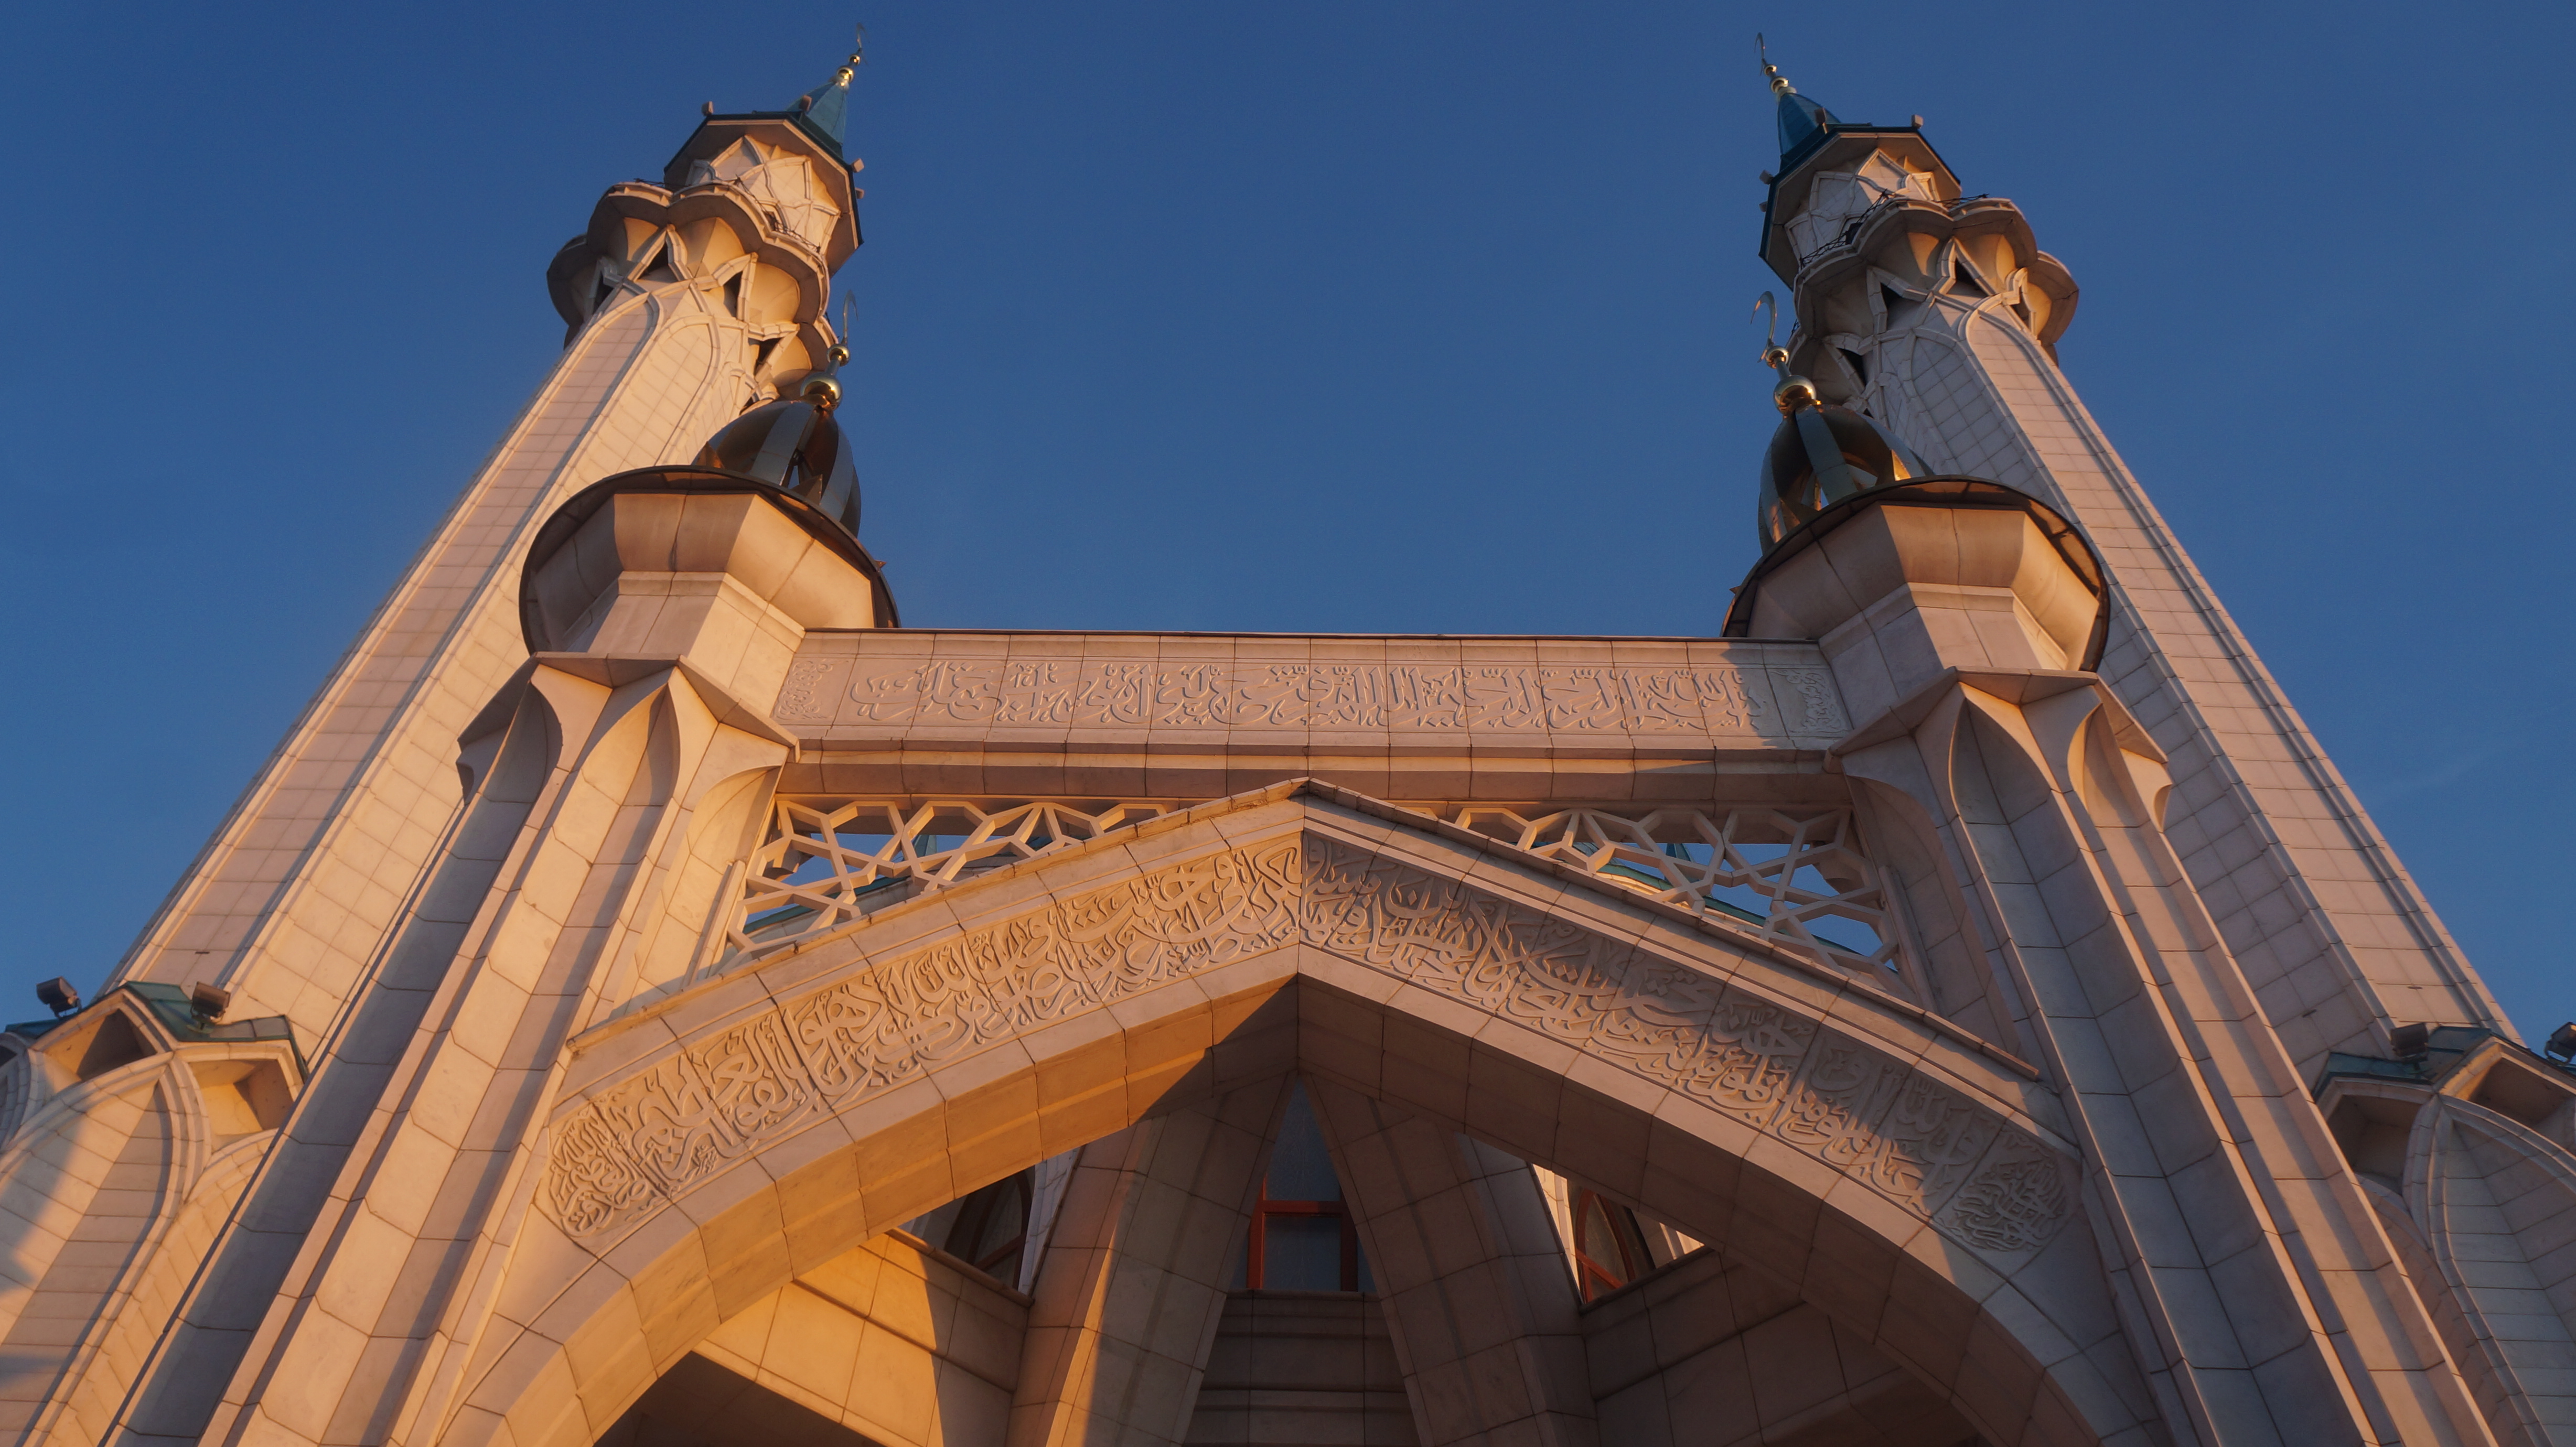
\includegraphics[width=130mm]{./imgs/kazan2.jpg}  
  %\hfill
\end{adjustwidth}
  \caption{Mesquita encravada no coração do Kremlin de Kazan}

\thispagestyle{empty}

\end{figure}
\end{vplace}

\end{absolutelynopagebreak}

%\clearpage{\pagestyle{empty}\cleardoublepage}
%\makeatletter\@openrightfalse
\movetooddpage
\addcontentsline{toc}{part}{Kazan [km 794]}
\part*{KAZAN -- KM 794\\\smallskip\small{(A LESTE DE MOSCOU E\\\vspace{-4pt}DE NÍJNI NOVGOROD)}}


\chapter*{Deus, Alá e a flor que murchou sua beleza como~um derradeiro ato de liberdade}
\addcontentsline{toc}{chapter}{[24/06/18] Deus, Alá e a flor que murchou sua beleza como um derradeiro ato de liberdade}
%\@openrighttrue\makeatother

\begin{flushright}
\emph{Kazan, 24 de junho de 2018}
\end{flushright}

Capital da República do Tartaristão, uma das repúblicas que formam a
Federação Russa, Kazan já me mostra seu sincretismo étnico"-religioso
junto à entrada do Kremlin local: uma inscrição, em cirílico e em árabe,
celebra a contribuição das profissões de fé ortodoxa e muçulmana para as
tradições da cidade. É assim que sobrenomes como Chamilov e Kiríllov
despontam em feições com olhos puxados e maçãs do rosto sobrelevadas,
traços típicos dos tártaros de origem asiática. {[}Bem capaz de
surpreender boa parte dos forasteiros, tal mescla não tem como deixar
este brasileiro boquiaberto, uma vez que a mestiçagem é a razão de ser
do nosso país -- do horror da escravidão de negros e índios pelos
portugueses ao ímpeto (até hoje dolosamente adiado) por uma verdadeira e
libertária democracia plurirracial.{]}

Cruzada a muralha caiada e altiva do Kremlin, logo deparo com a
escultura de um guerreiro tártaro de feições enrijecidas pela iminência
do combate. O traje militar, não de todo distinto de um quimono, é atado
por uma faixa, à altura da cintura. Com o braço esquerdo, o soldado
soergue um enorme escudo; a mão direita retém uma espada de lâmina curva
como a lua crescente islâmica -- eis o prenúncio da \emph{jihad}, a
guerra santa que os islâmicos tiveram o ímpeto de mover contra o tsar
Ivan, o Terrível, já que o adjetivo que veio a caracterizar o monarca
bem nos pode mostrar sua disposição em reprimir duramente os muçulmanos
que vinham professando sua fé bem antes da chegada da cruz (e das
tropas) ortodoxa(s).

Mas eis que, à revelia do déspota ortodoxo e em consonância com a
maioria da população de Kazan, que professa o islamismo, o Kremlin
abriga em suas muralhas uma mesquita de abóbada azul vivaz circundada
por quatro minaretes, em cujos topos a lua islâmica desponta voltada
para Meca. Como sói acontecer, trechos do Alcorão percorrem as paredes
da mesquita com a plasticidade dos caracteres árabes.

Como o Ocidente e suas (neo)cruzadas tendem a ter uma visão extremamente
limitante e limitada do islamismo, compartilho com os leitores e
leitoras do \emph{Diário de um escritor na Rússia} alguns trechos do
sermão de despedida do profeta Maomé, um dos textos religiosos mais
libertários com os quais já tive contato. Li tal sermão pela primeira
vez, em inglês, no pátio da Mesquita Azul, em Istambul, na Turquia; como
o Ocidente é cioso de sua própria genealogia para a construção dos
direitos humanos, os muçulmanos parecem (e não mais do que parecem)
desprovidos da possibilidade de alteridade e empatia. Não à toa,
entretanto, o sermão de despedida do profeta Maomé foi arrolado como um
prenúncio da Declaração Universal dos Direitos Humanos. Eis, então,
alguns fragmentos maometanos que ressoam e renovam as palavras mais
emancipatórias de Jesus Cristo:

\begin{quote}
Ó Povo, assim como consideram este mês, este dia e esta cidade como
sagrados, considerem a vida e a propriedade de todo muçulmano como
sagrados. Devolvam os bens que lhes forem confiados aos seus legítimos
donos. Não prejudiquem uns aos outros para que ninguém os prejudique.
Lembrem que encontrarão seu Senhor, e que Ele pedirá contas de seus
atos. Não devem infligir nem sofrer qualquer injustiça.

Ó Povo, é verdade que têm certos direitos em relação às suas mulheres,
mas elas também têm direitos sobre vocês. Lembrem que as tomaram como
esposas somente sob a custódia de Deus e com Sua permissão. Se elas
mantiverem os seus direitos, então a elas pertence o direito de ser
vestidas e alimentadas com gentileza. Tratem bem suas mulheres e sejam
gentis com elas, porque elas são suas parceiras e ajudantes dedicadas.

Toda a humanidade descende de Adão e Eva. Um árabe não é superior a um
não"-árabe, nem um não"-árabe tem qualquer superioridade sobre um árabe; o
branco não tem superioridade sobre o negro, nem o negro é superior ao
branco; ninguém é superior, exceto pela piedade e boas ações. Aprendam
que todo muçulmano é irmão de todo muçulmano e que os muçulmanos
constituem uma irmandade. Nada que pertença a um muçulmano é legítimo
para outro muçulmano a menos que seja dado de livre e espontânea
vontade. Portanto, não cometam injustiças contra vocês mesmos.

Lembrem que um dia se apresentarão perante Deus e responderão pelos seus
atos. Então fiquem atentos e não se desviem do caminho da retidão depois
que eu partir.
\end{quote}

A 100 metros da mesquita, deparo com uma igreja ortodoxa %(ou menos)
encimada por bulbos azuis, ao centro dos quais desponta um bulbo dourado
e sobrelevado representando a primazia de Deus.

Por séculos desde Ivan, o Terrível -- a mando de quem tal igreja
ortodoxa foi erigida --, o canal Bulac cindiu Kazan em duas metades
antagônicas: de um lado, os cristãos ortodoxos; do outro, os tártaros
muçulmanos. Se nos lembrarmos da águia bicéfala como símbolo da
monarquia tsarista, teremos que a águia voltada para o Ocidente (a
Europa) e a águia voltada para o Oriente (a Ásia) só não se devoravam
porque a coroa do tsar, pairando em meio a ambas para conter o potencial
fratricídio, (supostamente) suplantava e unificava as dissensões. Para
além, no entanto, do cetro monárquico -- e a despeito da nova aliança
(ou, melhor, da nova cumplicidade) entre Estado e ortodoxia sob Vladímir
Putin --, o Kremlin de Kazan dá o tom para a coexistência pacífica entre
cristãos e muçulmanos.

Ocorre que a convivência entre fiéis de credos distintos em meio aos
territórios russófilos pluriétnicos e plurirreligiosos tem um histórico
profundamente encarniçado.

Recorramos, então, à novela \emph{Khadji"-Murát}, de Tolstói, para, %Liev
em meio ao Cáucaso convulsionado por guerras étnico"-religiosas entre
cristãos e muçulmanos, entrarmos em contato com momentos cruciais da
vida do comandante regional Khadji"-Murát, rebelde que já lutara ao lado
do \emph{imame} Chamil, chefe caucasiano que, a partir de 1834, moveu
guerra aos russos durante 25 anos.

Quando o narrador de Tolstói nos apresenta Khadji"-Murát, o combatente se
debandara para o lado dos russos. A princípio, imaginamos que Murát
traíra Chamil pela vontade de poder, pois o (suposto) desertor já

\begin{quote}
imaginava como avançaria contra Chamil à frente do exército que {[}o
comandante russo{]} Vorontzóv lhe daria e como o faria prisioneiro;
depois, o tsar russo iria premiá"-lo, e ele governaria não só a Avaria,
mas toda a Tchetchênia por ele submetida\footnote{Liev Tolstói,
  \emph{Khadji"-Murát.} Tradução de Boris Schnaiderman. São Paulo:
  Editora 34, 2017, p. 52.}.
\end{quote}

Logo descobrimos que, em meio às disputas de poder, Chamil aprisionara
os familiares de Khadji"-Murát -- daí a guinada do rebelde em direção aos
cristãos e daí o ímpeto por vendeta. {[}Exímio conhecedor das
contradições humanas, Tolstói entrevê o altar da \emph{jihad} soerguido pela natureza profana dos homens.{]}
%(guerra santa)

Panoramicamente, eis os marcos narrativos de \emph{Khadji"-Murát.} Ocorre
que, junto com o fluxo da estória, o breve romance parece desvelar um
afã tolstoiano por cenários e costumes típicos do Cáucaso, afã que,
encadeado poeticamente à narrativa, chega a conferir estatura ontológica
às descrições, como se a natureza e a cultura do Cáucaso fossem elevadas
à condição de personagens. É assim que ``margaridas insolentes'' se
esgueiram entre ``malmequeres brancos e jeitosos, de pólen amarelo
vivo''; é assim que ``doía olhar para o aço das baionetas e para o
brilho, semelhante a pequenos sóis, que aparecia subitamente sobre o
bronze dos canhões''; é assim que a ``fragrância orvalhada da noite de
lua'' ressoa ``o canto e o silvo de alguns rouxinóis, vindos do jardim
pegado à casa''; é assim que a lembrança do avô de Khadji"-Murát, ``de
rosto enrugado e barbicha grisalha'', o obriga a proferir as orações
diárias com suas ``mãos de veias intumescidas''\footnote{Idem, p. 25;
  126-127; pp. 162-163; p. 166.}. {[}Em \emph{Khadji"-Murát}, a
sobreposição vertiginosa de descrições"-personagens como que transforma o
foco narrativo em tomadas fílmicas -- não à toa, o cineasta russo
Serguei Eisenstein apreendeu germes de narrativa cinematográfica em meio
à pulsão imagética de Tolstói.{]}

Em um breve preâmbulo a \emph{Khadji"-Murát}, o narrador nos diz que
tentara colocar uma bardana de haste rija e fibrosa no centro de um
ramalhete com as mais belas flores do Cáucaso. A bardana resistiu
vigorosamente à subjugação e, quando seu caule enfim se partiu, a flor
murchou sua beleza como um derradeiro ato de liberdade. Ao fim da
estória, o narrador retoma a imagem da bardana indômita como uma
metáfora para o destino de Khadji"-Murát, cuja vida premida entre a
dominação russa, a guerra santa e a vendeta pelos entes queridos o
transforma em uma personagem trágica, para quem, ainda que a morte seja
certa e iminente, é preciso fazer o elogio do próprio
naufrágio\footnote{Parte deste escrito compôs o meu texto ``Tolstói e a
  guerra do Cáucaso'', publicado em 08/07/17 no caderno literário
  ``Aliás'', do jornal \emph{O Estado de S. Paulo}.}.

\chapter*{Adeus, Lênin?}
\addcontentsline{toc}{chapter}{[25/06/18] Adeus, Lênin?}

\begin{flushright}
\emph{Kazan, 25 de junho de 2018}
\end{flushright}

Ao largo da Praça Vermelha, em Moscou -- a bem dizer, por todos os
cantos da capital russa e, provavelmente, em todas as cidades do país
--, é possível encontrar a {\MinionPro{матрёшка}} (\emph{matriochka}), uma boneca
multicolorida de madeira que se abre ao meio e de cujo ventre vão
saindo, sucessivamente, bonequinhas cada vez menores.

Na Rússia historicamente transpassada pelo culto ao grande líder, não
poderia faltar a \emph{matriochk}a política, é claro. Assim, da boneca
maior, representada pelo neotsar Vladímir Putin, à boneca menor,
encarnada pelo bolchevique Vladímir Lênin, as \emph{matriochki}
(emprego, aqui, o plural russo) vão acompanhando, da contemporaneidade
até os primórdios da Revolução de 1917, a sucessão inversa de
presidentes russos e premiês soviéticos.

Putin, então, engloba Boris Iéltsin, o primeiro presidente eleito após o
colapso da União Soviética que, por sua vez, contém Mikhail Gorbatchov,
o líder reformista que, ao tentar arejar a \versal{URSS} para dar uma face humana
ao socialismo, acabou sendo o último a apagar as luzes {[}até hoje,
alguns sovietófilos nostálgicos acusam Gorbatchov de alta traição;
ademais (e talvez já com três ou quatro talagadas de vodca a mais), há
quem acuse o carismático Gorbi, com sua característica mancha vermelha
sobre o cocuruto, de ser um maçom a serviço do imperialismo
estadunidense{]}.

Gorbatchov, por sua vez, engloba Leonid Brejnev, o longevo e sonolento
premiê que, com sua voz algo embargada, permaneceu no poder durante 18
anos -- de 1964 até o ano de sua morte (1982). {[}A \emph{matriochka}
política pula, na sucessão inversa de Gorbatchov a Brejnev, os
gerontocratas Konstantin Tchernenko e Iúri Andropov, que, devido à idade
bíblica, acabaram permanecendo durante muito pouco tempo à frente da
\versal{URSS}.{]}

Brejnev contém o carismático e bom de briga Nikita Khruschov, o
secretário geral do Partido Comunista que liderou a \versal{URSS} durante a
gravíssima crise dos mísseis em Cuba, em outubro de 1962, escaramuça
que, ao contrapor as duas superpotências da Guerra Fria, quase levou o
mundo ao apocalipse nuclear.

Khruschov, então, engloba Ióssif Stálin, o ditador que comandou a União
Soviética durante a Grande Guerra Patriótica contra os invasores
nazistas e que, por meio dos planos quinquenais, da
coletivização/inanição forçadas no campo, da política de extermínio e
expurgo dos (supostos) inimigos e da drenagem de trabalho escravo, levou
a \versal{URSS}, segundo uma de suas colocações mais pitorescas, ``do arado de
ferro à bomba atômica''.

A \emph{matriochka}/Kinder Ovo de Stálin, ao fim e ao cabo, dá à luz
Vladímir Lênin, o líder da Revolução de Outubro de 1917.

Mas, para aquém (e para além) do grande panorama histórico com seus
líderes máximos, como era a vida cotidiana (o microcosmo) em meio à
União Soviética?

A propaganda estadunidense durante a Guerra Fria (corroborada pelos
golpes militares profiláticos aplicados na América Latina com o
beneplácito dos \versal{EUA}) só fazia enfatizar o totalitarismo de Estado e a
falta de liberdades civis, o desrespeito aos direitos humanos, a
escassez de produtos nos mercados e as filas quilométricas para a
obtenção de alimentos. Mas, ao lado do teor de verdade de tais
colocações, como era a vida cotidiana (o microcosmo) em meio à União
Soviética?

Para tentar elucidar um pouco das expectativas e sonhos dos cidadãos e
cidadãs soviéticos, o Soviet Lifestyle Museum, aqui em Kazan, nos
apresenta um verdadeiro antiquário -- ou relicário, a depender da
coloração ideológica -- do cotidiano da \versal{URSS}.

Logo à entrada do museu, deparo com uma piada que atesta, para os
devidos fins, que o escritor tcheco Franz Kafka recebeu o título de
cidadão honorário da União Soviética. (Vale frisar que Kafka costumava
rir aos borbotões enquanto lia para os amigos suas estórias de sumo medo
a prenunciar o totalitarismo de Estado à direita e à esquerda.) Eis o
chiste:

\begin{quote}
\forceindent{}-- Alô, é da polícia?

-- Sim.

-- Aqui é o Vássia.

Breve ruído.

Em 5 minutos a campainha volta a soar.

-- Alô, é da polícia?

-- Sim.

-- Aqui é o Vássia.

Breve ruído.

5 minutos.

Campainha.

Voz junto à porta.

-- É o Vássia?

-- Sim.

-- Aqui é a polícia.
\end{quote}

Logo ao lado, leio um chiste que espia através do verniz oficial da
ética soviética do trabalho {[}a ética protestante (sem Deus) e o
espírito do socialismo{]}:

\begin{quote}
\forceindent{}-- Onde você trabalha, Ivan?

-- Em nenhum lugar.

-- Mas o que você faz?

-- Nada.

-- Mas que trabalho fantástico!

-- Sim, meu trabalho é fantástico -- mas a concorrência é enorme!
\end{quote}

E que dizer da cobrança dos pais soviéticos pelo bom desempenho de seus
filhos na escola? Com um sorriso de canto de boca, o Soviet Lifestyle
Museum nos dá uma dica:

\begin{quote}
\forceindent{}-- Paizinho, hoje na escola tem reunião de pais\ldots{} Mas é só pra alguns
pais.

-- Só para alguns pais? Como assim, Sacha?!

-- Sim\ldots{} A reunião é só pra você e pro professor.
\end{quote}

Em contraposição à aura cinzenta que a propaganda dos \versal{EUA} atribui à
\versal{URSS}, o museu desvela a vida soviética em seu lirismo risonho:

\begin{quote}
\forceindent{}-- Kátia, minha filha, o que você tá fazendo?

-- Tô escrevendo uma carta, mamãe.

-- Ora, menina, mas você ainda não sabe escrever!

-- E o que que tem? A minha amiga também não sabe ler.
\end{quote}

E que dizer quando uma mãe depara com o retrato de seu filho artista
quando bem jovenzinho?

\begin{quote}
\forceindent{}-- Mamãe, mamãe, eu tive um sonho muito lindo, mamãe! -- exclama o
pequeno Sacha.

-- E você sabe o que o sonho quer dizer, meu filho?

-- Claro que sei, mamãe. O sonho\ldots{} é o cinema enquanto dorme.
\end{quote}

Tornando o tempo e a memória tangíveis, o Soviet Lifestyle Museum
apresenta pôsteres os mais diversos -- da estátua idealizada do operário
brandindo o martelo ao lado da camponesa soerguendo a foice até as
admoestações (a bem dizer, as ordens) estatais para que os cidadãos não
fumassem e (como se adiantasse alguma coisa) não bebessem.

Jaquetas e camisetas, calças e tênis, broches, bolsas e adesivos com os
caracteres em russo, sempre grafados em vermelho, da \versal{CCCP} {[}Союз
Советских Социалистических Республик (\emph{Soiuz Sovietskikh
Sotsialistitcheskikh Respublik}), isto é, União das Repúblicas
Socialistas Soviéticas.{]}

Uma charge anônima mostra um enorme alicate com a estrela vermelha da
\versal{URSS} desmembrando as engrenagens decrépitas de um Hitler trêmulo e mal
preparado para enfrentar o General Inverno russo. Ao lado de um pôster
altivo do soldado soviético na Segunda Guerra -- {\MinionPro{За
Pодину, За Сталина, За Cвободу}}! (\emph{Za Rodinu, Za Stalina, Za Svobodu!}, isto é, Pela Vitória, Por Stálin, Pela liberdade!), vejo uma foto, em preto"-e"-branco,
de uma camponesa que acena, sorridente, da carroceria do trator de sua
fazenda coletiva -- provavelmente, a foto data dos anos 1960, quando
Khruschov, a partir de uma política de degelo antiestalinista, procurou
insuflar ímpeto de utopia rediviva na população com seu estímulo a
safras recordes no campo e a programas de construção coletiva de
edifícios a partir de blocos pré"-fabricados, para que cada família
soviética pudesse viver em seu próprio apartamento para além das
moradias coletivas.

Quem já leu o romance \emph{Doutor Jivago}, obra"-prima que rendeu ao
russo Boris Pasternak o Prêmio Nobel de Literatura em 1958, se lembrará
de que, não muito tempo depois da vitória dos bolcheviques, em outubro
de 1917, a enorme casa do médico (e poeta) Iúri Jivago foi expropriada e
passou a abrigar várias famílias em seus numerosos cômodos. {[}Não à
toa, um velho dito da finada República Democrática Alemã -- mais
conhecida, no Ocidente, como Alemanha Oriental -- sentenciava que uma
cozinha própria (isto é, uma cozinha não compartilhada com um sem"-número
de famílias) valia uma vida.{]}

Um pôster colorido em homenagem à parada do Dia 1º de Maio me permite
entrever a elegância austera das mulheres soviéticas, com seus vestidos
sem decotes -- não se veem nem mesmo ombros à mostra --, cinturas bem
talhadas e meias"-calças a realçar a silhueta até a comportada altura dos
joelhos. Carregando bexigas de várias cores, a molecada veste bermudas,
meias suspensas e camisas de botão com mangas compridas.

Um pôster do {\MinionPro{Коммунистический Cоюз Mолодёжи}} (\emph{Kommunistitcheski
Soiuz Molodioji}, isto é, União da Juventude Comunista), o Komsomol,
sentencia que o membro pré"-mirim, com seu lenço vermelho ao redor do
pescoço, deve estar ``Sempre pronto!'' -- {\MinionPro{Всегда готов}}!~(\emph{Vsegda
gotov!}) -- para as demandas do Partido. Com o braço estendido em
continência e a mão direita aberta em palma a cruzar a testa como se
fosse uma hipotenusa, a saudação do Komsomol já prepara o jovem membro
para a disciplina de caserna do socialismo. {[}Não à toa, um velho dito
do Partido Comunista da finada Alemanha Oriental assim sentenciava:
\emph{Die Partei hat immer Recht} (O Partido sempre tem razão).{]}

E eis que vejo uma foto de Mikhail Kalachnikov enviada pelo próprio
militar e engenheiro russo ao Soviet Lifestyle Museum. Datada de 09 de
novembro de 2013, véspera do 94º aniversário do lendário inventor do
fuzil de assalto \versal{AK}-47, Kalachnikov só viveria mais 44 dias depois de
capturada a imagem em que aparece de olhos algo esbugalhados e vestido
com uma jaqueta esportiva junto à sua mesa de trabalho. À esquerda (mas
também à direita), o \versal{AK}-47 passou a fazer parte das mais diversas
sublevações armadas pelo mundo -- após a guerra de independência em
relação a Portugal, Moçambique chegou a estampar o fuzil em sua bandeira
nacional.

Boletins escolares e gramáticas soviéticas; pistolas de plástico e
réplicas do \versal{AK}-47 em madeira; sobretudos e quepes do Exército Vermelho e
do \versal{KGB}; vitrolas e fitas cassete (músicas de época ficam tocando ao
fundo); perucas desgrenhadas e maços de cigarro amassados; centenas de
fotos de Gagárin e desenhos do cosmonauta com giz de cera; máscaras de
gás (para o caso sempre ``iminente'' de um ataque ianque) e até mesmo
uma bolsa, dos anos 80, com a imagem de um velho Lada -- no Parque
Lênin, nas cercanias de Havana, em julho de 2013, dirigi um Lada
vermelho cuja caixa de câmbio já não discernia entre a segunda e a
quarta marchas e cujos pneus, mais carecas que Lênin, ainda assim
freavam quando, já começando a suar, eu pisava no pedal até o talo.

Em 2008, enquanto eu fazia um curso de língua russa na {\MinionPro{Российский
Университет Дружбы Народов}} (\emph{Rossiiskii Universitet Drujby
Narodov}, Universidade Russa da Amizade dos Povos), um de meus
professores, o bigodudo Vitali Tchartoritcheski, traçou uma comparação
entre os novos e os velhos tempos.

-- Como nós, acadêmicos das humanidades, não tínhamos lá muito prestígio
em comparação com os cientistas e engenheiros que impulsionavam a
corrida armamentista e o programa aeroespacial da União Soviética, não
nos restava muito ímpeto para a criatividade -- isso sem falar na
liturgia do marxismo"-leninismo segundo a qual precisávamos rezar. Ainda
assim, chegamos a fazer alguns estudos pitorescos, por meio dos quais
descobrimos que Púchkin e Lênin, em termos de estatística vocabular,
eram de fato gênios: há mais de 10 mil palavras distintas -- se bem me
lembro, a cifra chega a 15 mil -- empregadas por eles ao longo de suas
obras, veja só! E, bom, se você estiver pensando que tais estudos são
frutos de quem não tem muito mais o que fazer, ouça essa: a época atual
-- sobretudo vocês, do Brasil, mas também a velha Europa -- se gaba por
encher estádios para jogos de futebol; pois então saiba, meu caro, que,
na União Soviética, nós lotávamos estádios para ouvir poesias -- sim,
para ouvir poemas e recitá"-los: chegávamos ao êxtase coletivo não com
gols, mas com versos e estrofes de Púchkin e Maiakóvski, veja só! Como é
que eu vou esquecer que, em outubro de 67, no 50º aniversário da
Revolução, mais de 70 mil pessoas reunidas no Estádio Central Lênin
reverberaram versos de Maiakóvski -- versos que os marinheiros recitavam
enquanto, de seus encouraçados, eles investiam contra o palácio de
inverno do tsar, em São Petersburgo, durante a Revolução: ``Come ananás,
mastiga perdiz. / Teu dia está prestes, burguês''. Naquele momento, meu
caro, nós acreditamos que a beleza salvaria o mundo. Sim, nós
acreditamos, nós acreditávamos! Vamos, me chame hoje de ingênuo e de
idiota, mas nós tínhamos algo -- um sentido tangível -- para além de
contas bancárias e redes de \emph{fast food.} E o que vocês têm hoje,
meu caro? Vamos, me diga: o que vocês têm?!

O Soviet Lifestyle Museum e a lembrança das palavras de Vitali me fazem
aterrissar, sem mais, no filme \emph{Adeus, Lênin!}, dirigido pelo
alemão Wolfgang Becker. Ao fim da narrativa, Alex, filho bastante
amoroso da dedicada comunista Christiane, precisa enterrar a mãe
cardiopata que não conseguiu sobreviver ao colapso do bloco socialista.
O enterro de Christiane, no entanto, não relegará a utopia a sete palmos
do chão. Alex procura, ainda uma vez, o afago da memória. Na extinta
Alemanha Oriental, as crianças, como se fossem cosmonautas, lançavam
seus foguetes lúdicos com a esperança de que o socialismo fosse o
pioneiro na exploração do espaço. Christiane pede a Alex que suas cinzas
sejam lançadas aos céus a bordo de um foguete cosmonauta -- o Vostok 1
de Iúri Gagárin. Quiçá para distanciá"-la de um mundo em que a utopia se
transformara em estilhaço da memória. Adeus, Lênin. Quiçá para se
confundir com as estrelas, cujo firmamento distante a humanidade tentou
redesenhar com o socialismo.

Ao fim e ao cabo, a viagem cosmonáutica pelos escombros da memória e da
utopia me faz entender uma colocação sumamente espirituosa e
contraditória, nostálgica e (por que não?) lírica de Vladímir Putin,
quando o ex"-agente do \versal{KGB} assim sentenciou a jornalistas russos em
meados de 2010: ``Aquele que quer restaurar a União Soviética não tem
cérebro, mas quem não lamenta o seu fim não tem coração''.
%\footnote{Deparei
 % com a citação de Putin como epígrafe da obra \emph{Limonov}, do
  %escritor francês Emmanuel Carrère. Tradução de Sérgio Teles. Rio de
  %Janeiro: Alfaguara, 2016, p. 7.}.

\clearpage{\pagestyle{empty}\cleardoublepage}
\movetooddpage
\addcontentsline{toc}{part}{A bordo do trem que vai de Kazan a Saransk}
\part*{A BORDO DO TREM QUE VAI DE\\KAZAN A SARANSK}

\chapter*{Confesso que sobrevivi:\\Tolstói, suicídio e redenção}
\addcontentsline{toc}{chapter}{[26/06/18] Confesso que sobrevivi: Tolstói, suicídio e redenção}

\begin{flushright}
\emph{Entre Kazan e Saransk, 26 de junho de 2018}
%\emph{A bordo do trem que vai de Kazan\\a Saransk, 26 de junho de 2018}
\end{flushright}

A 10 km do centro de Kazan (se tanto), chego ao Templo de Todas as
Religiões: trata"-se de um complexo (passando por múltiplas reformas) que
contém duas igrejas -- uma ortodoxa, outra católica --, uma mesquita,
uma sinagoga e um centro animista que retoma práticas religiosas
antiquíssimas em meio aos tártaros.

As cruzes católicas e ortodoxas, a estrela de Davi e a lua islâmica
coexistem sobre bulbos e tetos policromáticos, como se cada uma dessas
tradições não quisesse tomar para si a primazia do céu.

Súbito, deparo com um velho careca e de barba desgrenhada vestindo uma
túnica preta e puída que lhe chega aos calcanhares. Seus olhos bem azuis
e estreitos como frestas só não se mostram mais vivazes que seus punhos
em riste: o velho fala com ímpeto e vigor -- ao redor do pregador
grisalho, dezenas de pessoas o ouvem com um silêncio extático de árvores
perfiladas em um bosque.

Com a mão direita, sobre cujo dorso despontam nódoas marrons e veias
intumescidas, o velho só faz brandir uma pequena obra autobiográfica do
escritor russo Liev Tolstói: \emph{Uma confissão}. Como se trata de um
livro de minha inteira predileção, aprumo os ouvidos para escutar a
pregação do velho, que se posta de maneira equidistante em relação a
todos e a cada um dos centros religiosos.

-- Assim falou Liev Nikoláievitch Tolstói: ``O que vai ser daquilo que
faço hoje e daquilo que vou fazer amanhã -- o que vai ser de toda a
minha vida? Para que devo viver, para que fazer algo? Existe, em minha
vida, algum sentido que não seria aniquilado pela morte
inevitável?''\footnote{Liev Tolstói, \emph{Uma confissão}. Tradução de
  Rubens Figueiredo. São Paulo: Mundo Cristão, 2017, p. 44-45.}

Tais perguntas existencialmente inescapáveis estão no coração de
\emph{Uma confissão}. (O velho pregador agita a obra em direção a seus
ouvintes com entusiasmo.)

-- Acossado pelo espectro do suicídio, o consagrado autor de
\emph{Guerra e paz} e \emph{Anna Kariênina} reconfigura o dilema de
Hamlet: se quem muito pensa sobre a vida cedo ou tarde depara com a
morte, \emph{ser e não ser}, para Liev Nikoláievitch Tolstói, não podem
transformar as respostas em lápides.

-- Aristocrata riquíssimo, Liev Nikoláievitch Tolstói já fizera uma
crítica radical à sua classe social, ao chamar a todos (e, sobretudo, a
si mesmo) de parasitas que, apartados da busca pelo sentido da vida, só
faziam chafurdar na luxúria que o privilégio da exploração alheia lhes
permitia.

-- Autor consagrado internacionalmente -- a vida do conde"-escritor era
rastreada por jornalistas ávidos por indiscrições e escândalos (eis os
avós dos atuais \emph{paparazzi}) --, Liev Nikoláievitch Tolstói já
fizera uma (auto)crítica radical aos escritores que, sempre envolvidos
em querelas e escaramuças, só faziam jactar"-se pelo apreço do público e,
assim, desviavam"-se das questões últimas da existência e reduziam a
literatura a uma forma sofisticada de ludibrio.

-- É assim que, em meio a uma torrente tão profunda quanto rara de
autocrítica, abnegação e lucidez, as confissões de Liev Nikoláievitch
Tolstói recorrem a um conto oriental para tentar desvelar o sentido da
vida a ser ceifada pela morte.

-- Imaginemos um viajante que, enquanto cruza a estepe, se vê perseguido
por um animal feroz. Para se salvar da fera, o viajante pula em um poço
seco, ao fundo do qual há um dragão ávido para devorá"-lo. Para evitar a
morte certa, o viajante se agarra aos ramos de um arbusto silvestre que
lograra crescer através das fissuras do poço. Ocorre que suas mãos
começam a ceder, e o viajante sente que logo precisará se entregar para
a morte, já que o animal feroz lhe barra a saída, e o dragão faminto lhe
veda o abrigo ao fundo do poço. (Para este conto oriental, chegar ao
fundo do poço é, de fato, uma noção para otimistas.)

-- E eis que o viajante, ao olhar para os lados, vê um rato branco (o
dia) e um rato preto (a noite) perambulando junto ao arbusto -- o frágil
galho que sustenta o viajante vai sendo roído pelos ratos do tempo.

-- Ocorre que, em meio às folhas do arbusto, o viajante descobre uma
gota de mel e passa a lambê"-la com sofreguidão, como se a ilusão do
prazer fugaz pudesse ludibriar a morte certa. É quando Liev
Nikoláievitch Tolstói arremata o conto oriental: ``Porque vejo com
clareza o dragão, o mel já não me traz doçura. Vejo só uma coisa -- o
dragão inevitável e os ratos -- e não consigo desviar meus olhos. E isso
não é uma lenda, isso é a verdade, inquestionável e entendida por
todos''\footnote{Idem, pp. 39-40.}.

-- Mas eis que Liev Nikoláievitch Tolstói, inquieto e inquisitivo por
excelência, nos envolve em um novo turbilhão de perguntas: ora, se a
consciência da morte (ou, pior, a consciência para a morte) aniquila o
sentido racional da vida; se, como quer o sumo pessimismo do filósofo
alemão Arthur Schopenhauer, o nada anterior à existência teria sido
preferível à vida, de modo que o retorno ao nada, com a morte, seria o
único bem em meio a uma vida repleta de choro e ranger de dentes; se, em
suma, o suicídio é a única ação racional para uma vida desprovida de
qualquer sentido, como é que a humanidade, desde sempre acossada pelo
espectro da morte, ainda não se aniquilou? Como é que os homens e
mulheres, desde tempos imemoriais, vêm logrando viver sem se suicidar?

-- É quando Liev Nikoláievitch Tolstói, alçando"-se para além do inferno
suicida, descobre o caráter quintessencial -- a bem dizer, ontológico --
da fé. A fé, Liev Nikoláievitch Tolstói nos confessa, ``não é apenas o
`desvelamento de coisas invisíveis', não é só a relação do homem com
Deus -- a fé é o sentido da vida humana, graças ao qual o homem não se
destrói e vive. Se o homem vive, ele acredita em alguma coisa. Se não
acreditasse que é preciso viver para alguma coisa, ele não
viveria''\footnote{Idem, pp. 79-80.}. Para Liev Nikoláievitch Tolstói, a
fé não move montanhas -- a fé nos faz escalá"-las. A fé no sentido para
além da morte, a fé em que a morte é uma transição, a fé na eternidade.

\pagebreak

-- Ora, como Schopenhauer não se matou, Liev Nikoláievitch Tolstói bem
poderia dizer que a publicação de \emph{O mundo como vontade e
representação}, obra magna do filósofo alemão, foi um ato de fé. Para
além da floresta negra de seu pessimismo, Schopenhauer afirmou a vida
com o ímpeto que o fez erigir sua obra. Assim, as confissões de Liev
Nikoláievitch Tolstói insinuam que Schopenhauer não poderia sentenciar
que não teve filhos e que não transmitiu a nenhuma criatura o legado de
nossa miséria\footnote{Parte significativa deste escrito compôs o meu
  texto ``A vida como profissão de fé para o mestre russo'', publicado
  em 08/07/17 no caderno literário ``Aliás'', do jornal \emph{O Estado
  de S. Paulo}.}.

%\pagebreak
\clearpage
\thispagestyle{empty}

\movetoevenpage
\begin{absolutelynopagebreak}
\begin{vplace}
\begin{figure}[H]
\begin{adjustwidth}{-1.8cm}{}
  %\centering
  \vspace{2.7cm}
  %\hspace{0.3cm}
  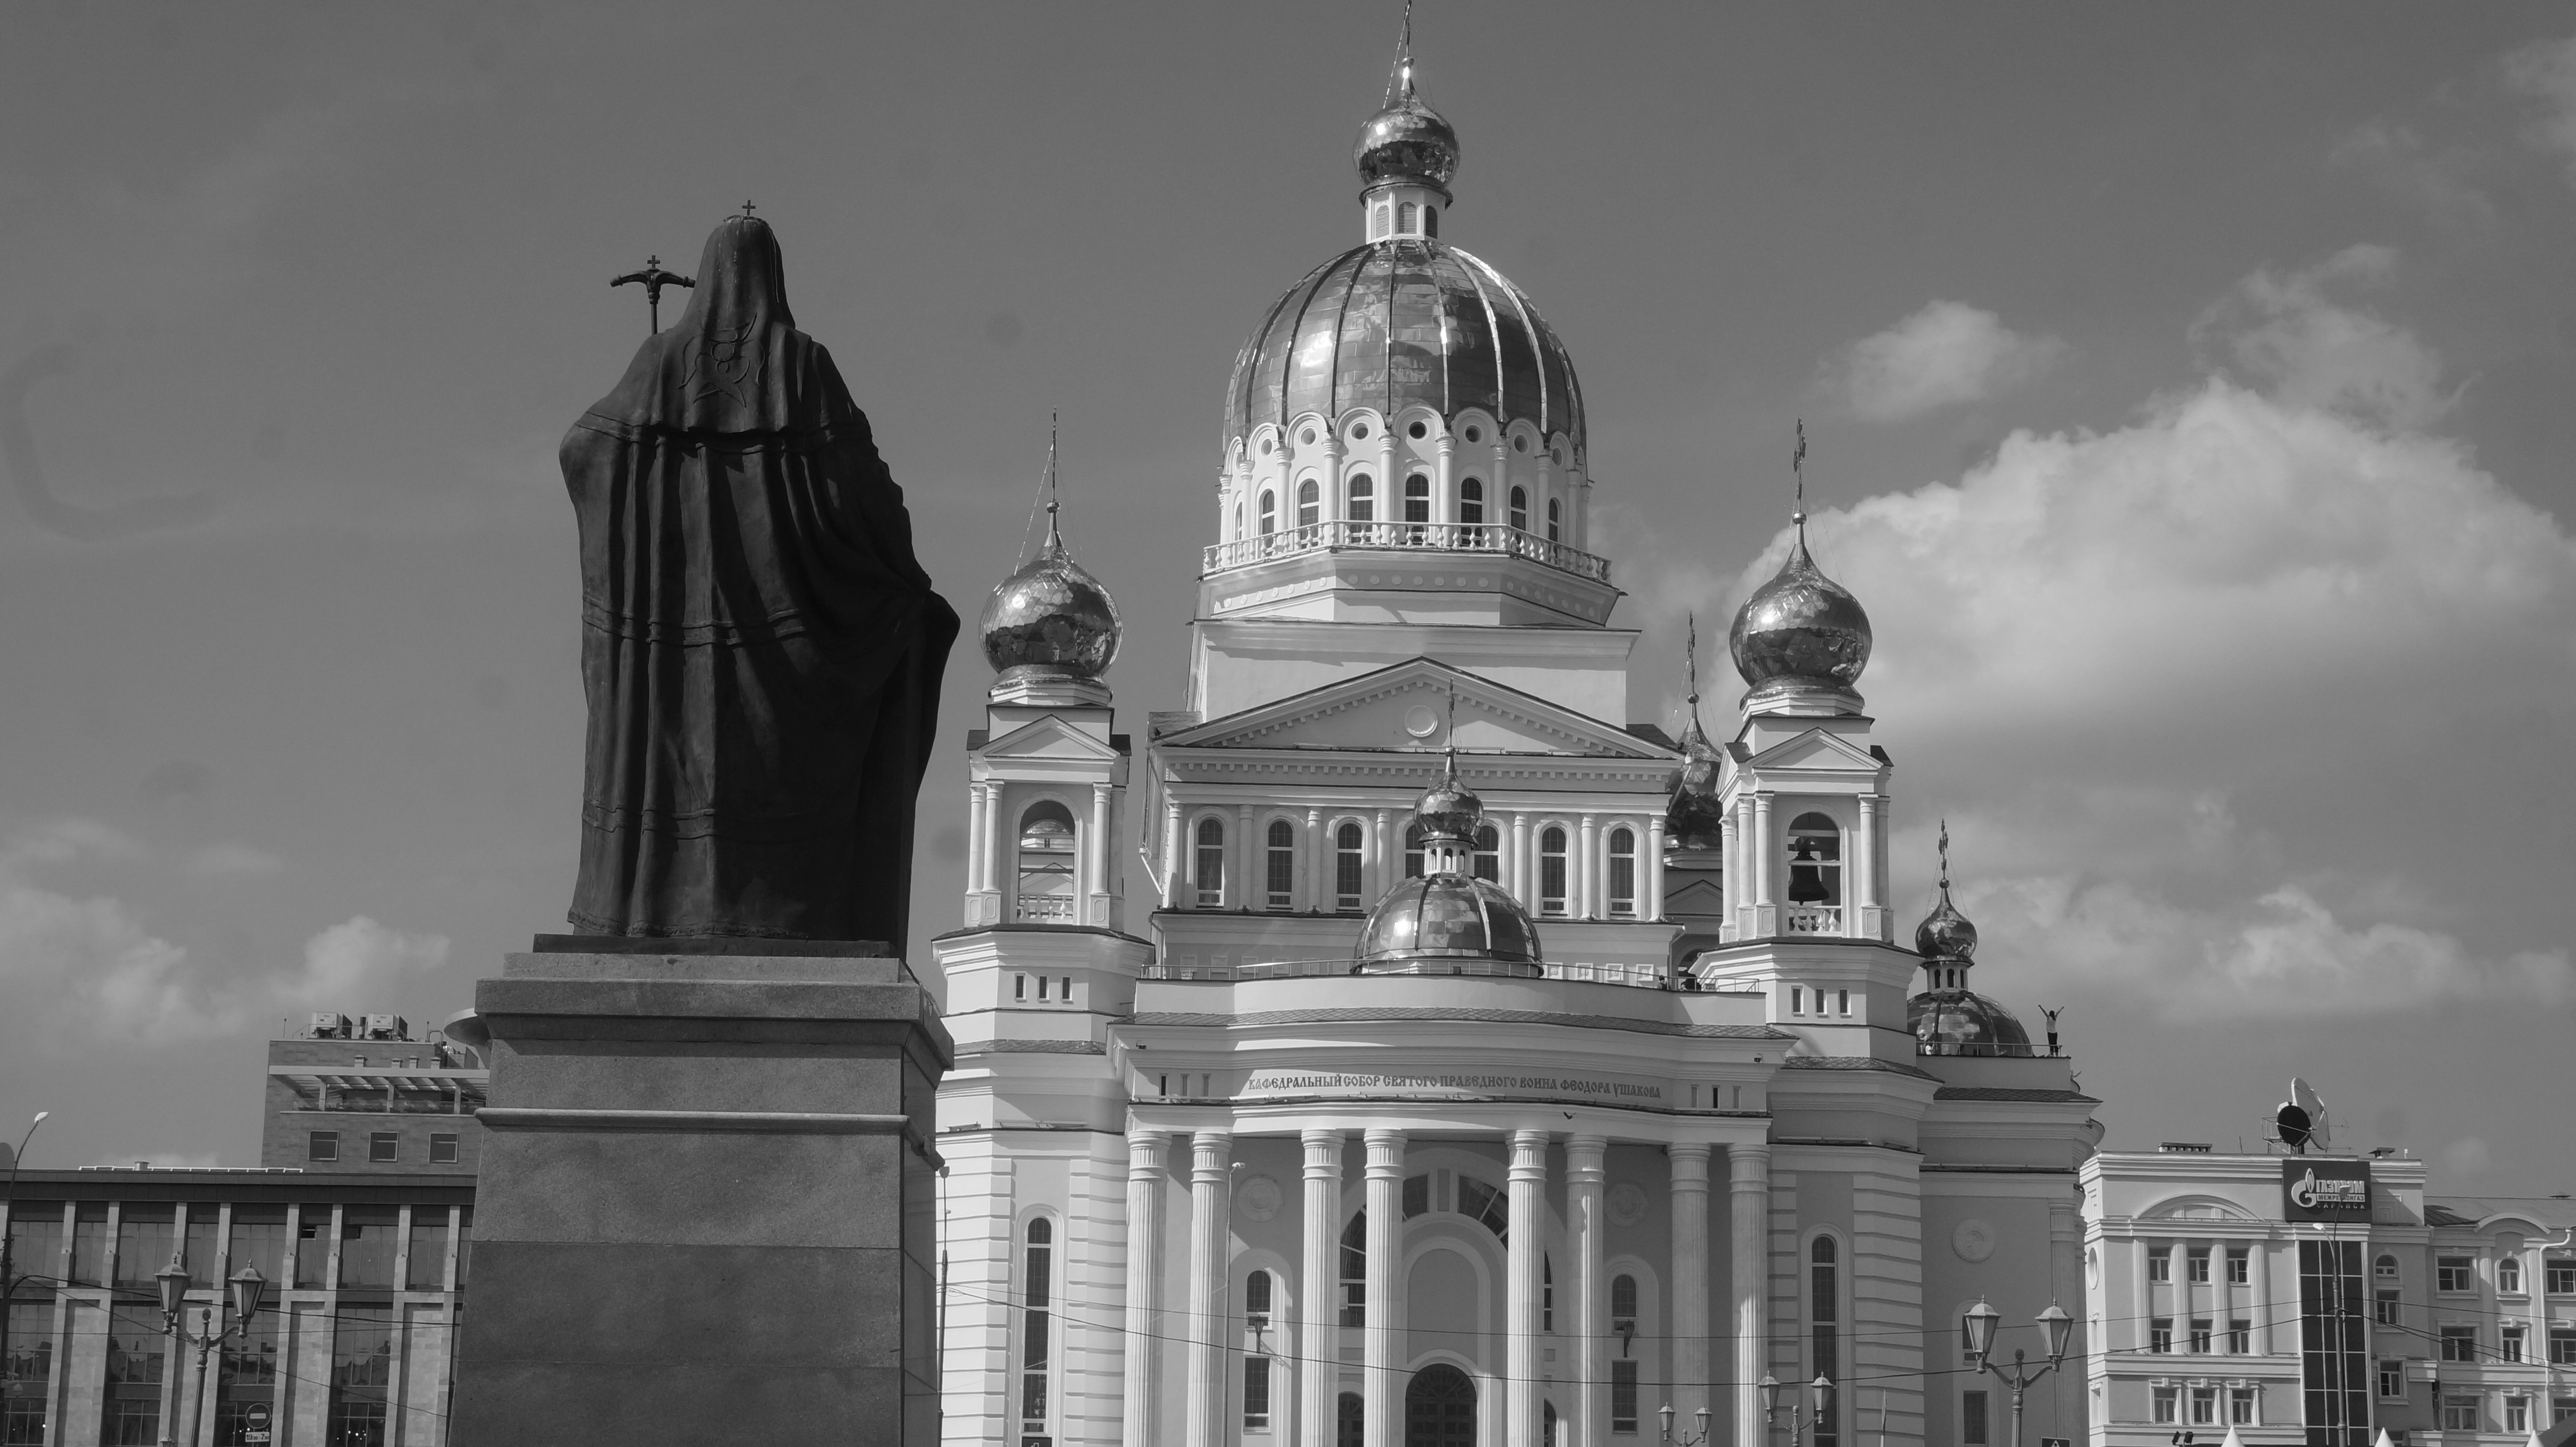
\includegraphics[width=130mm]{./imgs/saransk1.jpg}  
  %\hfill
\end{adjustwidth}
  \caption{Catedral ortodoxa de Saransk guarnecida por um patriarca da Igreja russa}

\thispagestyle{empty}

\end{figure}
\end{vplace}

\end{absolutelynopagebreak}

%\clearpage{\pagestyle{empty}\cleardoublepage}
%\makeatletter\@openrightfalse
\movetooddpage
\addcontentsline{toc}{part}{Saransk [km 1164]}
\part*{SARANSK -- KM 1164\\\smallskip\small{(A SUDESTE DE MOSCOU; AO\\SUL DE NÍJNI NOVGOROD; A\\\vspace{-4pt}SUDOESTE DE KAZAN)}}


\chapter*{Eu sou eu e minha circunstância: Os animais sociais de Fiódor Dostoiévski e Mikhail Bakhtin}
\addcontentsline{toc}{chapter}{[27/06/18] Eu sou eu e minha circunstância: Os animais sociais de Fiódor Dostoiévski e Mikhail Bakhtin}
%\@openrighttrue\makeatother

\begin{flushright}
\emph{Saransk, 27 de junho de 2018}
\end{flushright}

A aproximadamente 650 km a leste de Moscou, a cidade de Saransk, capital
da República da Mordóvia, abrigou o teórico da literatura e filósofo da
linguagem russo Mikhail Bakhtin durante o longo e intermitente exílio a
que o autor foi submetido pelas autoridades soviéticas entre as décadas
de 1930 e 60.

Em 1929, Bakhtin publica a primeira versão de \emph{Problemas da poética
de Dostoiévski}, obra que pode ser lida como uma crítica tão velada
quanto radical à ditadura soviética capitaneada por Stálin. %Ióssif

Bakhtin considera que a obra de Fiódor Dostoiévski logrou desvelar a
condição ontologicamente dialógica dos homens e mulheres, na medida em
que as personagens despontam como vozes que forjam sua subjetividade em
estreita articulação com a voz (a pergunta e a dúvida, a hesitação, a
réplica e a tréplica) do outro. Segundo Bakhtin, o universo de
Dostoiévski não está povoado de personagens cujos conjuntos de valores e
tensões se insulam em si mesmos, como se Ródion Románovitch Raskólnikov,
(anti-)herói do romance \emph{Crime e castigo}, estruturasse sua
subjetividade como um castelo fortemente resguardado em relação à
alteridade e às crises que o transpassam. Nada seria mais estranho a
Dostoiévski (e a Bakhtin) do que o seguinte aforismo do filósofo
austríaco Ludwig Wittgenstein: ``Os limites da minha língua são os
limites do meu mundo''\footnote{Ludwig Wittgenstein, \emph{Tractatus
  logico"-philosophicus}. Tradução de José Arthur Giannotti. São Paulo:
  Companhia Editora Nacional, 1968, p. 111.}.

Nesse sentido, antes de aterrissarmos na obra de Dostoiévski, vale a
pena fazermos três breves digressões, em diálogo com os alemães Karl
Marx e Werner Herzog e com o português José Saramago, para melhor
compreendermos os pressupostos da condição dialógica dos homens e
mulheres. A partir, então, da recente greve dos caminhoneiros ocorrida
no Brasil, falemos sobre o que vem a ser a ontologia do ser social.

No primeiro volume de \emph{O capital}, Marx cita um velho provérbio
alemão --\emph{Mitgefangen, mitgehangen} (Presos juntos, juntos
enforcados) -- para falar que, em meio à moderna sociedade capitalista
de produção de mercadorias, a profunda e coercitiva divisão do trabalho
nos faz conviver segundo a lógica~da ``dependência coisificada
universal''\footnote{Karl Marx, \emph{O capital.} Tradução de Flávio
  Kothe. São Paulo: Nova Cultural, 1998, p. 95.}. Quando um setor vital
e radicalmente capilarizado da divisão social do trabalho -- em nosso
caso, a circulação mercantil por meio de caminhões -- estanca suas
atividades, todos aqueles e aquelas que se veem como indivíduos
autossuficientes (como castelos resguardados de sua própria vontade e
representação) aprendem que, em sua impotência para dar sequência à
reprodução do cotidiano, a individualidade só existe relacionalmente,
isto é, vinculada aos demais nós da rede que nos entrelaça.
\emph{Mitgefangen, mitgehangen} (Presos juntos, juntos enforcados).

No \emph{Ensaio sobre a cegueira}, o ateu José Saramago\footnote{José
  Saramago, \emph{Ensaio sobre a cegueira.} São Paulo: Companhia das
  Letras, 1995.} lança mão de um elemento sobrenatural (a cegueira
branca) para escarafunchar a dinâmica mais recôndita da realidade: eis o
paradoxo estético que faz com que a realidade, escavada pela ficção,
seja mais real, tangível e cognoscível. Quando a cegueira branca
despenca como um raio em céu azul, os ramos da divisão social do
trabalho, um a um, vão entrando em colapso. A sociedade, mais uma vez,
se impõe em relação à suposta e radicalmente ideológica (no sentido de
falseamento da realidade) independência do indivíduo. Cegos juntos,
juntos enforcados.

No filme \emph{O enigma de Kaspar Hauser}, direção de Werner Herzog,
Kaspar é o filho bastardo de um nobre que, para evitar o escândalo
cortesão, enclausura o filho em uma torre e priva"-lhe da possibilidade
de socialização. O pai apenas visita o filho para lhe dar comida. Os
anos vão passando, e o pai de Kaspar, um belo dia, tem a ideia de
ensinar o filho a escrever. Como todas as mediações lógico"-sociais
faltam às vivências de Kaspar, o rapaz mal sabe o que é postar"-se de pé
e articular palavras -- que dirá, então, idealizar conceitos para
exprimi"-los concretamente sobre o papel. Simbolicamente, o pai ordena
que o filho escreva o verbo \emph{schreiben} (escrever). Como a
metalinguagem pressupõe a vivência social da lógica linguística anterior
à palavra escrita e para além do âmbito propriamente gráfico, Kaspar mal
consegue deslizar o lápis sobre o papel e, como um papagaio, só faz
remedar o verbo"-ação que o pai tenta inculcar no filho:
\emph{sch"-rei"-ben}. Como seria possível, então, afirmar a
individualidade como algo alheio à ontologia do ser social? Bastardos
juntos, juntos enforcados.

Os limites da minha língua (e da minha subjetividade) são os limites do
meu mundo, como teria dito Ludwig Wittgenstein? Nada seria mais estranho
a Dostoiévski (e a Bakhtin) do que tal aforismo. Pensemos, nesse
sentido, sobre as profundas agonias morais por que passa o jovem
Raskólnikov, o (anti-)herói do romance \emph{Crime e castigo}.

Antena da raça (e de sua época), Raskólnikov apreende a potencial morte
histórica de Deus em meio ao século \versal{XIX} da Revolução Industrial e do
cientista inglês Charles Darwin. Assim, para ser coerente com o novo
culto niilista, o jovem intelectualmente intrépido resolve fazer um
experimento para descobrir se está à altura do relativismo ético de sua
época. Raskólnikov quer matar o \emph{Não matarás}.

Raskólnikov, então, decide assassinar Alióna Ivánovna, a usurária cuja
existência sem sentido só faz explorar a tudo e a todos. Um homem
extraordinário como Napoleão Bonaparte -- assim raciocina Raskólnikov
--, aquele para quem tudo é permitido, sequer hesitaria diante de um
piolho como Alióna Ivánovna.

Eis que Raskólnikov, munido de um machado, rasga a cabeça de Alióna
Ivánovna -- e da irmã da velha usurária que, coincidente e
inusitadamente, aparece no local do crime. Estamos, neste momento,
precisamente no fim da primeira parte de \emph{Crime e castigo}. Todo o
desdobramento posterior do romance gira em torno das agonias que
Raskólnikov passa a sentir diante do duplo homicídio -- o castigo em
face do crime.

Agora, se tivéssemos que refletir sobre as agruras de Raskólnikov em
termos de sua (re)configuração subjetiva e dialógica, como o faríamos?
Vejamos: sempre houve crimes na história da humanidade, então
Raskólnikov não acaba de inventar a roda, isto é, há jurisprudência
narrativa para o duplo homicídio, de tal maneira que a crise, nesse
sentido, não irrompe como uma completa impossibilidade de
significação/intelecção para os crimes.

Ocorre que, para Raskólnikov -- ou, melhor, para a época niilista de
Raskólnikov --, não se trata apenas de um mero crime, mas de um teste
relativista -- a morte do \emph{Não matarás}. Com o sangue aspergido por
seu machado, Raskólnikov se imagina o fundador de uma nova era, isto é,
já não podemos prever os desdobramentos narrativos para uma ação que
pretende ressignificar o ato mesmo que profana a lei e os profetas. Por
esse prisma, a crise de Raskólnikov após o duplo homicídio pode ser
entendida como a colisão de várias tensões, para além de sua própria
subjetividade, que não conseguem enformar uma nova narrativa para
reconciliar o jovem com seu novo eu. Após o duplo homicídio, Raskólnikov
se tornou, dialogicamente, um outro para si mesmo.

Ora, uma coisa é conceber um assassinato; outra, realizá"-lo. Os homens e
mulheres reais, seres de carne e osso que dialogam e que vão se forjando
social e historicamente, vivem os tabus e interditos erigidos pelas
sociedades. Infringir tais tabus e interditos, em termos de configuração
identitária, significa proceder a uma completa reviravolta narrativa e
dialógica para a compreensão de si mesmo. É assim que, após o duplo
homicídio, Raskólnikov se torna um outro para si mesmo.

Se o indivíduo abrisse a janela do (suposto) castelo resguardado de seu
eu, ele ouviria os gritos de dor e desespero de Raskólnikov por já não
entrever um princípio de contiguidade e continuidade entre seu eu
anterior e seu eu assassino -- não à toa, a maestria de Dostoiévski dá
vazão a fluxos e influxos de consciência lancinantes que quebram a
linguagem e fazem com que os leitores (e o próprio Raskólnikov) já não
saibamos quem está enunciando a crise (se o narrador em terceira pessoa,
se o próprio torpor de Raskólnikov). Ademais, Raskólnikov é um jovem
inteligente, vaidoso e cioso de sua valentia. A crise por causa do fardo
de ter aspergido sangue alheio também se vê transpassada pela vergonha
de não suportar o fardo de ter aspergido sangue de outrem.
{[}Raskólnikov, então, não estaria à altura de Napoleão, o jovem não
seria um ser extraordinário, para quem tudo é permitido, mas um ser
ordinário vivendo sob a tutela (arbitrária) da lei e dos profetas mesmo
após a potencial morte de Deus.{]}

O mergulho radical no cosmos de Dostoiévski fez com que Bakhtin
desdobrasse a condição dialógica dos homens e mulheres de modo a
entrever (e a entreouvir) o mundo como um concerto polifônico, em meio
ao qual as múltiplas vozes, sem poder definir as demais a partir de si
mesmas, pressuporiam a convivência democrática para a expressão de suas
mais variadas perspectivas; sendo radicalmente transpassado pelo outro
em sua condição, o eu, conforme Bakhtin procura demonstrar, deveria ser
visto como o eu"-outro -- a bem dizer, \emph{nós.}

Qualquer tentativa de definir o (e de ditar os rumos do) eu"-outro a
partir de perspectivas que lhe são radicalmente exteriores e heterônomas
só faria estancar e silenciar a dialogia que, para Bakhtin, nos é
constitutiva. A condição radicalmente antípoda à dialogia ontológica do
eu"-outro que, em termos globais, dá vazão a concertos polifônicos é a
ditadura encarniçada. Os censores soviéticos de Bakhtin bem entreviram
que \emph{Problemas da poética de Dostoiévski} pressupunha outro tipo de
sociedade -- a democracia polifônica para além do stalinismo -- para
que a verdadeira dialogia humana pudesse ser vivenciada em suas mais
diversas implicações e ramificações.

Não à toa, a 2ª edição da obra de Bakhtin sobre Dostoiévski só
sairia em 1963, dez anos após a morte de Stálin, quando a \versal{URSS}, então sob o governo do premiê Nikita Khruschov, procedia a autocríticas e à tentativa de degelo das estruturas estatais
totalitárias.
%segunda edição; só seria publicada em; quando a União Soviética


Para além do contexto stalinista que condenou Mikhail Bakhtin ao
exílio, é possível dizer que as premissas ontológico"-políticas de
\emph{Problemas da poética de Dostoiévski} ainda possuem profunda
atualidade. Os inimigos da democracia, agora sob o capitalismo, parecem
cada vez mais disseminados. Para todos aqueles e aquelas que se aferram,
contra sua própria condição dialógica e plural, a determinadas formas
identitárias, noções como horizontalidade e diversidade -- diversidade
ideológica e social, diversidade étnica e religiosa, diversidade de
gênero e de orientação sexual -- parecem blasfêmias em face da tradição
hierárquica, monológica e ossificada de sociedades como a russa e a
brasileira.

Como o diálogo bakhtiniano com Dostoiévski nos pôde demonstrar, a
(re)configuração da subjetividade pressupõe não apenas o diálogo com o
outro, cuja presença nos tranpassa (como animais sociais que somos), mas
também a dimensão de que a vida e suas inúmeras contingências se
apresentam para o eu, em enorme medida, como um quarto escuro em que se
vai tateando sem que seja possível saber, ao certo, aonde (e como) se
vai chegar. Quando se aferram a visões de mundo e a padrões de
identidade e comportamento estritos, as tendências antidialógicas e
autoritárias pretendem tornar estanque e arquetípica a subjetividade
que, ao longo da vida, é muito mais plástica e amorfa do que muitas
doutrinas e liturgias, à esquerda e à direita, gostariam de admitir.
Assim, é como se os espectros de Dostoiévski e Bakhtin rondassem o
imaginário de José Ortega y Gasset, quando o filósofo espanhol define,
de forma indefinida e indefinível, o processo de constituição de nossa
subjetividade dialógica: ``Eu sou eu e minha circunstância''\footnote{José
  Ortega y Gasset, \emph{Meditaciones del Quijote.} Madrid: Ediciones
  Cátedra, 1984, p. 69.}.

\chapter*{Almas mortas: saudade}
\addcontentsline{toc}{chapter}{[28/06/18] Almas mortas: saudade}

\begin{flushright}
\emph{Saransk, 28 de junho de 2018}
\end{flushright}

Com pouco mais de 300 mil habitantes, Saransk é uma pequena cidade --
não tão pequena quanto a Quintana de meus ancestrais, no interior de São
Paulo, com seus 5 mil habitantes (se tanto) --, cujo centro consigo
perfazer a pé.

Entre a catedral azulada e de bulbos dourados e o hotelzinho onde estou
hospedado, vejo alguns casebres à beira do rio com um estilo que só se
encontra na Rússia -- e, devo dizer, na Rússia profunda.

Imagine um tronco cortado ao meio, só que longitudinalmente.

Imagine, agora, uma sucessão justaposta de tais metades de troncos, uma
sobre a outra, como se baguetes abertas estivessem sendo perfiladas. Eis
a fachada dos casebres menos altos do que compridos.

Aqui em Saransk, a superfície dos troncos foi polida, o que lhes confere
uma impressão menos rústica. Em meados do ano passado, quando estive na
longínqua Sibéria -- em Ulan"-Ude, capital da República da Buriátia, ou,
então, ao longo da linha férrea do Grande Expresso Transiberiano, nas
imediações do lago Baikal --, vi casebres cujos troncos cascudos e
cheios de farpas pareciam recém"-extraídos da taiga, ainda que se
tratasse de moradias imemoriais.

Ouço o sino da catedral (ou imagino ouvi"-lo) e me vem à memória uma
passagem do romance \emph{Almas mortas}, do russo Nikolai Gógol, em meio
à qual a experiência do viajante nômade (fiel como os pássaros
migratórios) se funde à tentativa de compilar os retalhos bucólicos (da
toalha de mesa costurada pela avó?) de uma Rússia profunda em direção a
cujo passado a visão dos casebres me levou.

Eis o que a nostalgia gogoliana nos narra:

\begin{quote}
Assim que a cidade ficou para trás, logo se desenharam, de ambos os
lados da estrada, as bagatelas a que estamos {[}a que estávamos,
Gógol\ldots{}{]} acostumados: morrinhos, bosques de abetos, arbustos baixotes
de pinheiros jovens e raquíticos, troncos queimados de pinheiros velhos,
matagal bravo e outros disparates semelhantes. Apareceram vilarejos que
se estendiam como cadarços, construídos como se fossem antigos montes de
lenha, cobertos por telhados cinzentos, abaixo dos quais havia ornatos
de madeira entalhados nos beirais, que acabavam parecendo toalhas
bordadas pendentes. Alguns mujiques, como de hábito, bocejavam, sentados
em bancos diante dos portões, em seus casacos de pele de carneiro.
Camponesas, de cara gorda e peitos enfaixados, olhavam pelas janelas do
primeiro andar; nas janelas da parte de baixo, um bezerro espiava ou um
porco punha para fora seu focinho cego\footnote{Nikolai Gógol,
  \emph{Almas mortas.} Tradução de Rubens Figueiredo. São Paulo: Editora
  34, 2018, p. 406.}.
\end{quote}

À diferença de um Fiódor Dostoiévski, cujas obras são vistas pela
fortuna crítica como um paisagismo dos estados convulsos e escatológicos
da alma, Nikolai Gógol verte suas almas mortas para o caráter vivaz e
telúrico da Rússia profunda, trazendo à tona um mosaico folclórico de
que os leitores citadinos à época do capitalismo nascente (primeira
metade do século \versal{XIX}) começavam a se apartar. Um espectro de nostalgia
bucólica ronda o romance de Gógol, bucolismo que a Rússia tende a
comunicar ao Brasil, já que, guardadas as diferenças, ambos os países
periféricos passaram por processos de modernização, êxodo rural e
urbanização tardios em comparação com as nações centrais do capitalismo.
É assim que Nikolai Gógol e suas \emph{Almas mortas} parecem ter dado à
luz toda a nostalgia do chilreio dos pássaros, do galo da aurora e dos
pés descalços sobre o orvalho matutino; do moedor de café acoplado à
mesa de madeira rústica e da saudação com o chapéu de palha ao camponês
que volta da lavoura (``Taaarrrde!''); do coador de pano para o café
(muitas vezes, uma meia velha) e das cinzas ainda fumegantes do fogão à
lenha; do doce de abóbora com cravo da bisavó e dos acordes dos grilos
quando o escuro começa a despencar; do bule de café chiando e do leite
quente cheio de nata na caneca de alumínio retorcido do bisavô; da
bênção e do beijo de boa noite da avó antes que o sono venha sobre o
travesseiro de pena de ganso (ou seria de galinha?).

A nostalgia bucólica de \emph{Almas mortas} alcança o estatuto de uma
ontologia do tempo perdido. A ourivesaria do detalhe, em Gógol, tenta
estancar o fluxo irredimível do tempo com o mosaico (e o afago) da
memória, o canto fúnebre de uma Rússia que, enquanto agoniza, ainda
entoa a paisagem (e a aragem) de seu passado.

Agora pela manhã, aqui em Saransk, volto a ouvir as badaladas do sino da
catedral (ou imagino ouvi"-las).

Tomado, subitamente, pela noção (dostoievskiana) de que a beleza salvará
o mundo, me ocorre que a pergunta ``Por quem os sinos dobram?'' só pode
ser feita por alguém que se vê cindido da experiência mesma de
despertar, singelamente, com a aurora dos sinos.

A impossibilidade de transmitir em sua totalidade a aura dessa
experiência me levou, sem mais, à epifania que o alemão Martin Heidegger
chamou de ``acontecimento'' -- a meu ver, um dos mais belos acordes
poéticos da filosofia.

Tudo aquilo que acontece como epifania; tudo aquilo que irrompe com a
beleza dos olhos marejados; tudo aquilo que cicatriza com o ímpeto da
reconciliação; todo encontro que se consuma com a esperança da comunhão
-- acontecimentos assim (res)guardam sua aura na vivência mesma, de modo
que qualquer relato (qualquer soslaio narrativo) que tente se acercar do
momento necessariamente o faz sem carregar consigo o eriçamento
ontológico que o badalar dos sinos provoca em quem o ouve \emph{aqui e
agora}.

Em uma época que relega Deus ao exílio -- refiro"-me à busca verdadeira e
profunda por sentido e transcendência, e não aos vendilhões do templo à
frente de seus megaempreendimentos religiosos --, a noção heideggeriana
de ``acontecimento'' irrompe com a essência de tudo aquilo que é
místico, indômito e radicalmente subjetivo.

Por quem os sinos dobram, então? Por aquele que sente o afago de suas
badaladas. {[}Me ocorre, \emph{aqui e agora}, que o Príncipe Míchkin,
herói do romance \emph{O idiota} e fusão dostoievskiana de Jesus Cristo
e Dom Quixote, só pode ter sentenciado que a beleza salvará o mundo em
meio à aurora do verão russo que vai banhando os bulbos sinuosos das
catedrais ortodoxas com luz e sentido\footnote{Parte deste escrito
  compôs o meu texto ``A nostalgia bucólica de Gógol na aurora do
  moderno'', publicado em 07/07/18 no caderno literário ``Aliás'', do
  jornal \emph{O Estado de S. Paulo}.}.{]}

\clearpage{\pagestyle{empty}\cleardoublepage}
\movetooddpage
\addcontentsline{toc}{part}{A bordo do trem que vai de Saransk a Samara}
\part*{A BORDO DO TREM QUE VAI DE\\SARANSK A SAMARA}

\chapter*{Do Gulag siberiano ao iPhone, o arame farpado passa a cercear a imaginação}
\addcontentsline{toc}{chapter}{[29/06/18] Do Gulag siberiano ao iPhone, o arame farpado passa a cercear a imaginação}

\begin{flushright}
\emph{Entre Saransk e Samara, 29 de junho de 2018}
%\emph{A bordo do trem que vai de Saransk\\a Samara, 29 de junho de 2018}
\end{flushright}

Só os dogmáticos não veriam a reversão da utopia em distopia e da
revolução em Estado policial e escravidão após a leitura de
\emph{Arquipélago Gulag}, obra"-prima do escritor russo Alexander
Soljenítsin, premiado com o Nobel de Literatura em 1970.

A sigla Gulag refere"-se à Administração Geral dos Campos de Trabalho
Correcional e Colônias, um eufemismo para a criminalidade estatal que,
durante o auge da repressão sob o punho de Ióssif Stálin, sequestrou e
prendeu, assassinou, deportou e escravizou milhões de inocentes na União
Soviética. O arquipélago Gulag, nesse sentido, diz respeito a um
verdadeiro sistema de articulação entre múltiplos campos de trabalhos
forçados espraiados pela Sibéria e órgãos de espionagem e repressão --
na sociedade soviética acossada pelo stalinismo, as arbitrariedades se
capilarizavam da onipresença da polícia política até as delações
cotidianas feitas por vizinhos e professores, amantes e amigos.

Os sobreviventes cujas cartas municiaram a obra de Soljenítsin relatam
que os carrascos siberianos coagiam os prisioneiros a trabalhar a -40ºC.
Quando o General Inverno fustigava os condenados a -45ºC, a compaixão
dos verdugos suspendia os trabalhos em prol do respeito aos direitos
humanos. Não à toa, Soljenítsin sentencia que, em meio à pátria do
Gulag, ``quem diz lei diz crime''\footnote{Alexander Soljenítsin,
  \emph{Arquipélago Gulag.} Tradução de Antônio Pescada. Lisboa:
  Sextante Editora, 2017, p. 121.}.

É assim que, para a repressão stalinista, tudo o que é sagrado é
profanado. Eis o que Soljenítsin nos revela sobre o niilismo soviético:

\begin{quote}
Nada existe de sagrado na busca do domicílio! Quando prenderam o
maquinista ferroviário Vitkónski, encontrava"-se no quarto uma criança
que acabara de morrer. Os ``juristas'' não se furtaram a revistar o
corpo da criança. Eles dão safanões nos doentes de cama e tiram as
ligaduras que lhes cobrem as feridas. (\ldots{}) Um encanador desligava o
rádio do seu quarto sempre que transmitiam intermináveis cartas a
Stálin. Um vizinho denunciou"-o (onde estará agora esse vizinho?) como
elemento socialmente perigoso: oito anos de prisão. (\ldots{}) As prisões
políticas no nosso país singularizaram"-se pelo fato de serem detidas
pessoas em nada culpadas e, por isso mesmo, despreparadas para oferecer
resistência\footnote{Idem, p. 69.}.
\end{quote}

Se quisermos refletir, sem dogmatismo, sobre as tragédias históricas --
ou, pior, sobre a história como tragédia -- que deportaram a utopia da
sociedade soviética, deveremos nos lembrar de uma admoestação de
Soljenítsin: ``Aquele que recorda o passado perde um olho! E, no
entanto, o provérbio acrescenta: aquele que o esquece perde os
dois!''\footnote{Idem, p. 171.} Sendo assim, como esquecer que a pujança
do capitalismo ocidental se assentou, historicamente, sobre o dorso da
escravidão? Como esquecer que o ouro extraído com o sangue e o suor
negros das Minas Gerais acabou financiando, com a mediação colonial de
Portugal e Inglaterra, a eclosão da Revolução Industrial? (Aqueles que
conhecem os descaminhos da história -- ou, pior, a história como
descaminho -- não deixam de admirar a e de sentir calafrios diante da
beleza de Ouro Preto, cidade elevada a patrimônio cultural da
humanidade. Desde seu nome, Ouro Preto funde a beleza à culpa, o belo ao
bélico.)

Ademais, os ataques atuais à democracia mundo afora, aliados ao radical
desenvolvimento tecnológico, nos permitem pensar que os organismos de
espionagem e repressão da finada União Soviética já se tornaram
anacrônicos. Com a ubiquidade dos satélites, \emph{drones} e algoritmos
para rastrear conversas \emph{online} e \emph{offline}, o direito à
privacidade transforma"-se em um fóssil relegado a futuros arqueólogos.
Nesse sentido, eis o que nos diz o historiador israelense Yuval Noah
Harari, autor de \emph{Homo Deus: Uma breve história do amanhã}, obra
que pode ser interpretada como uma versão atualíssima do
\emph{Arquipélago Gulag}:

\begin{quote}
Hoje, nos Estados Unidos, há mais gente lendo livros digitais do que
impressos. Dispositivos como o \emph{Kindle} são capazes de coletar
dados de seus usuários enquanto eles estão lendo o livro. O seu
\emph{Kindle} pode monitorar quais partes do livro você lê depressa ou
devagar; em que página ou frase você abandonou a obra. Se o
\emph{Kindle} tiver um \emph{upgrade} para reconhecimento facial e
sensores biométricos, pode saber como cada frase influencia seu
batimento cardíaco e sua pressão sanguínea. O que o faz rir, o que o
deixa triste e o que lhe provoca raiva. Logo os livros estarão lendo
você enquanto você os lê. E, considerando a possibilidade de você
esquecer rapidamente a maior parte do que lê, o \emph{Kindle} jamais
esquecerá nada a seu respeito\footnote{Yuval Noah Harari, \emph{Homo
  Deus: Uma breve história do amanhã.} Tradução de Paulo Geiger. São
  Paulo: Companhia das Letras, 2016, p. 346.}.
\end{quote}

\pagebreak

Diante da colonização da mente para muito além da submissão do corpo, as
instâncias atuais de poder nos fazem sentir a nostalgia do Gulag.
Afinal, como resistiremos à dominação que transforma as sentinelas dos
antigos campos de concentração em arame farpado ao redor de nossa
imaginação?\footnote{Este escrito compôs o meu texto ``Gulag, uma
  tragédia para não ser esquecida'', publicado em 03/02/18 no caderno
  literário ``Aliás'', do jornal \emph{O Estado de S. Paulo}.}

%\pagebreak
\clearpage
\thispagestyle{empty}

\movetoevenpage
\begin{absolutelynopagebreak}
\begin{vplace}
\begin{figure}[H]
\begin{adjustwidth}{-2.7cm}{}
  %\centering
  \vspace{-1.8cm}
  \hspace{2.6cm}
  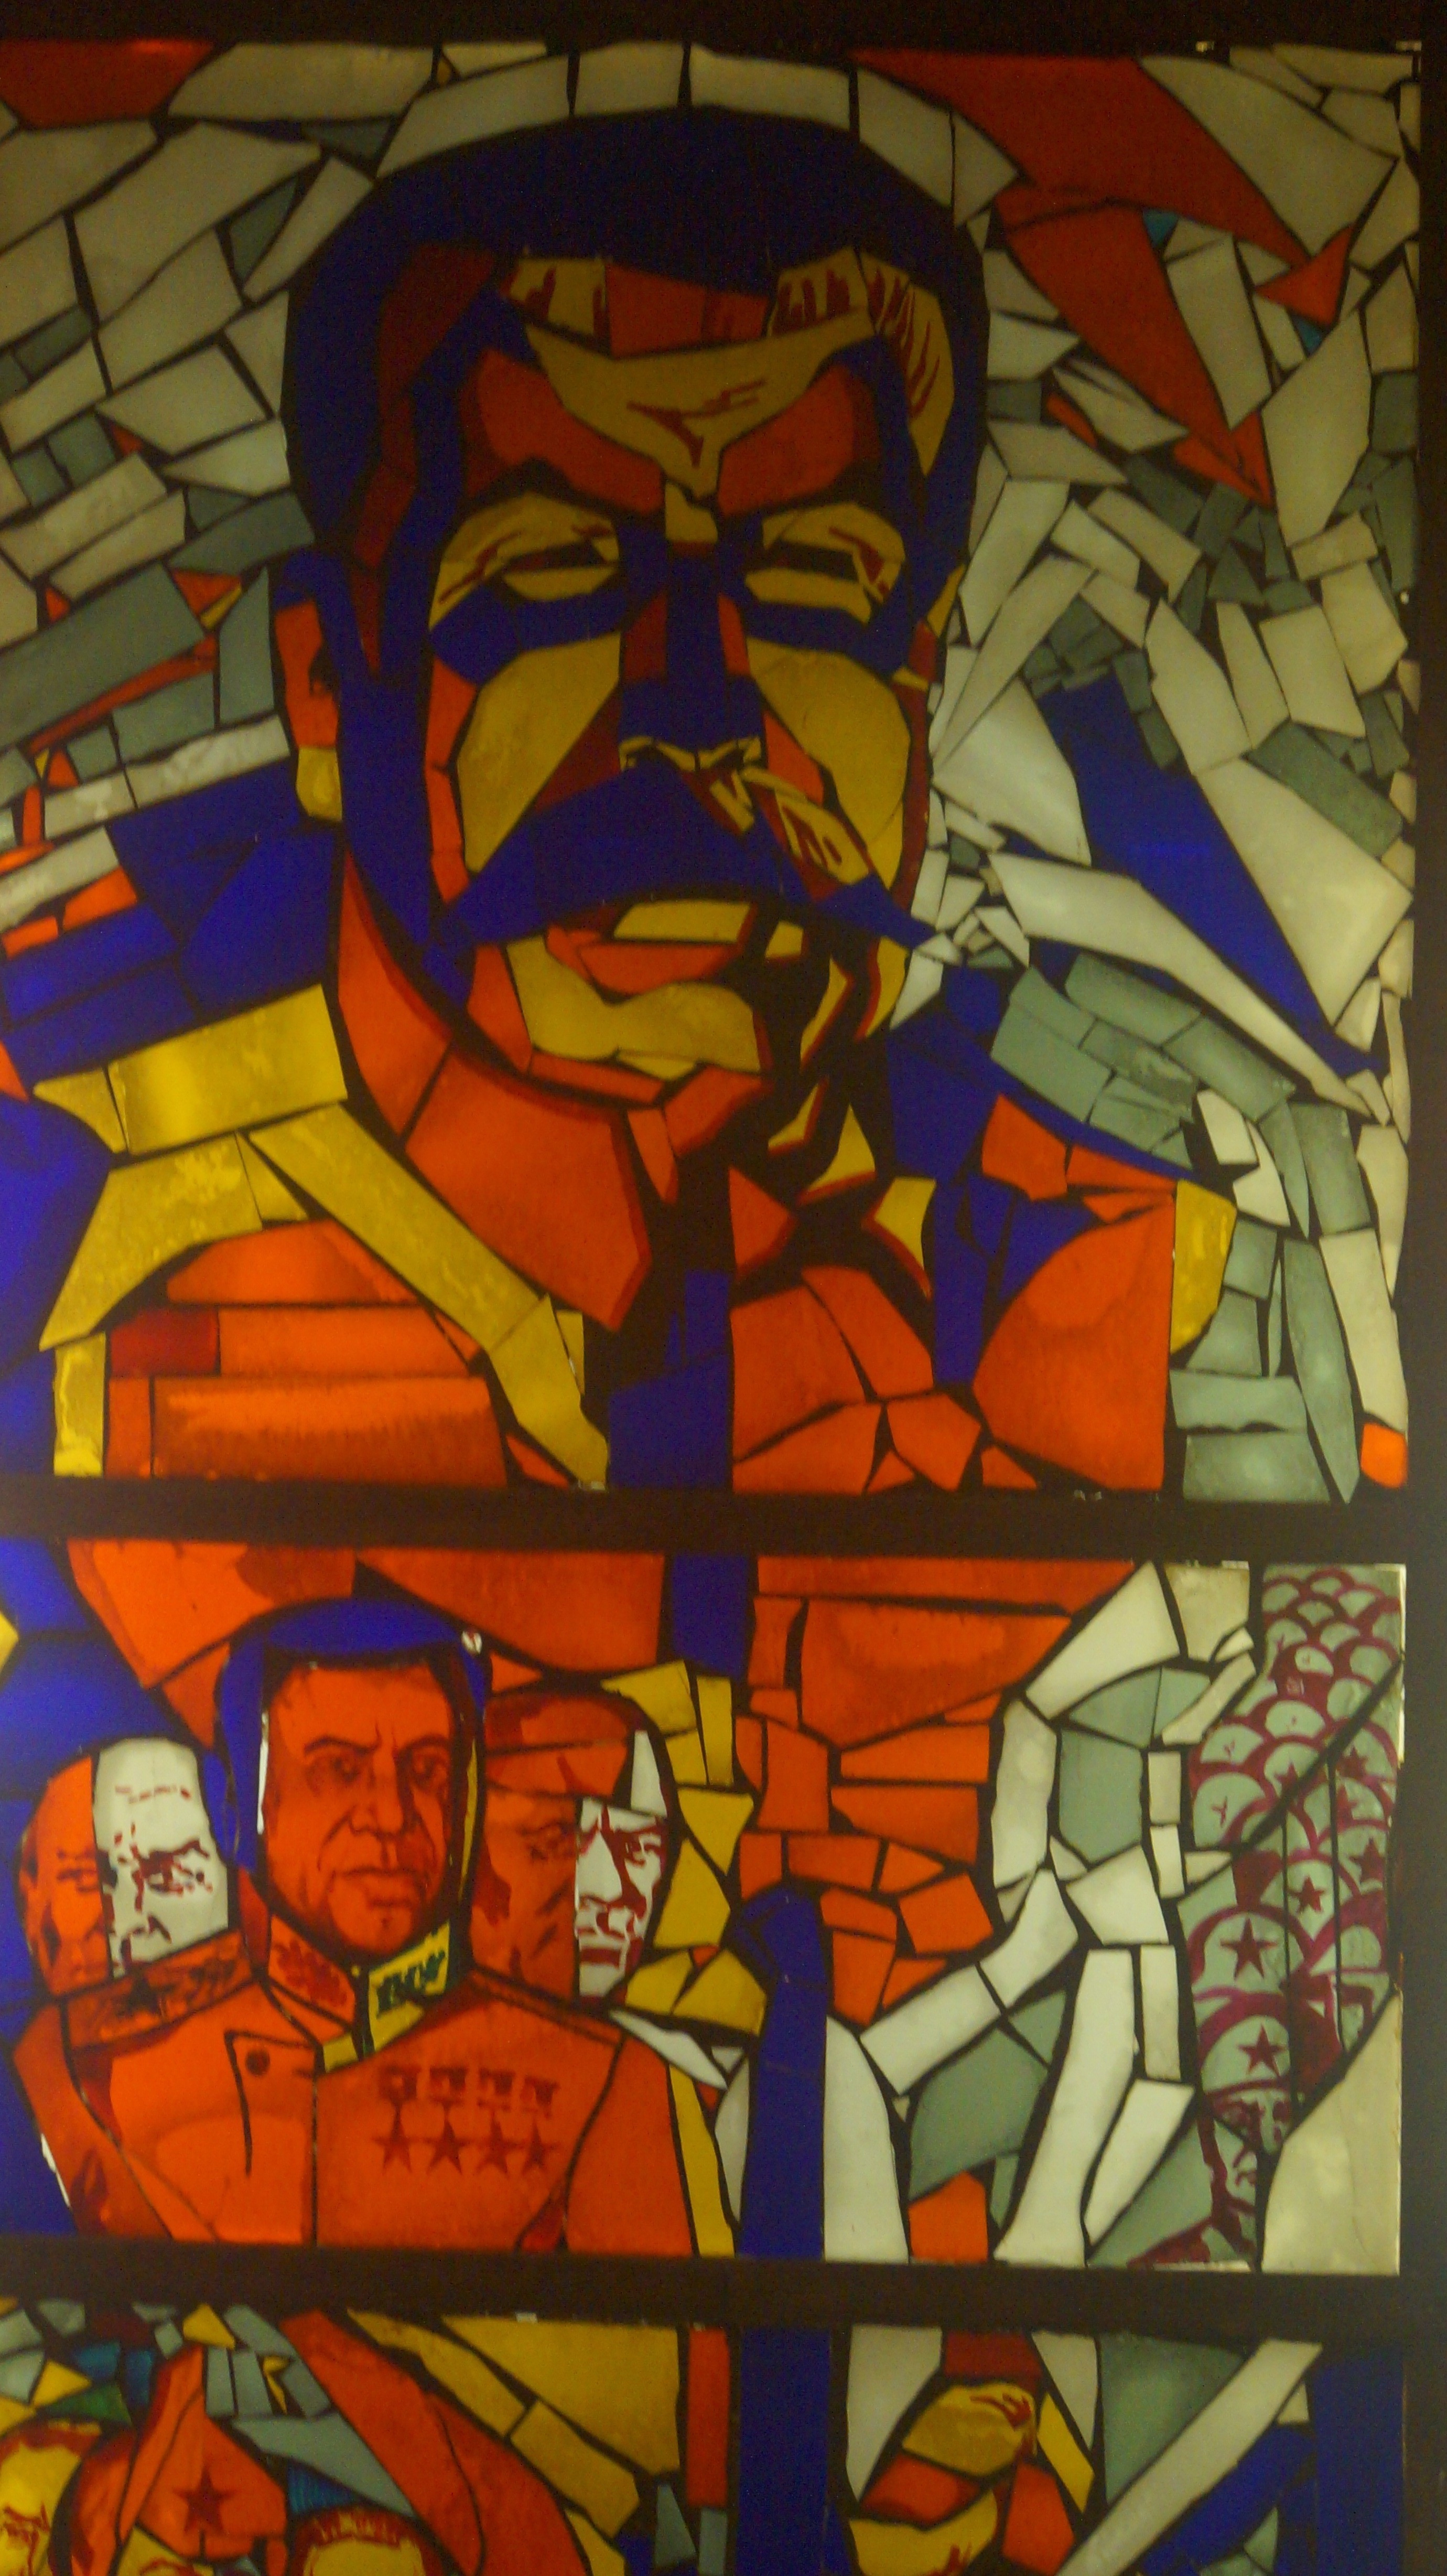
\includegraphics[width=95mm]{./imgs/samara1.jpg}  
  %\hfill
\end{adjustwidth}
\centering
\captionsetup{justification=centering}
    \caption{Vitral em homenagem ao ditador soviético Ióssif Stálin (1878--1953) à~entrada~de~seu~bunker,~em~Samara}

\thispagestyle{empty}

\end{figure}
\end{vplace}

\end{absolutelynopagebreak}

%\clearpage{\pagestyle{empty}\cleardoublepage}
%\makeatletter\@openrightfalse
\movetooddpage
\addcontentsline{toc}{part}{Samara [km 1593]}
\part*{SAMARA -- KM 1593\\\medskip\small{(A SUDESTE DE MOSCOU, NÍJNI\\NOVGOROD E SARANSK;\\\vspace{-4pt}AO SUL DE KAZAN)}}


\chapter*{Réquiem para Stalingrado:\\Matarás o próximo como a ti mesmo}
\addcontentsline{toc}{chapter}{[30/06/18] Réquiem para Stalingrado: Matarás o próximo como a ti mesmo}
%\@openrighttrue\makeatother

\begin{flushright}
\emph{Samara, 30 de junho de 2018}
\end{flushright}

Acabei de acordar, suado e palpitante, como se o coração estivesse
martelando o esterno: sonhei com Stalingrado, cidade para onde eu vou
daqui a 2 dias; cidade"-síntese para o \emph{front} mais letal da
história das guerras; cidade cuja batalha disputada rua a rua, ruína a
ruína, soldado a soldado começou a reverter o curso da Segunda Guerra
Mundial contra os piratas nazistas.

Stalingrado está toda asfixiada pelos caças e tanques -- a mão"-garrote
enforca o pescoço das estradas, o coturno cheio de lama pisa sobre o
graveto frágil da sobrevivência.

Todos os escombros do mundo -- grandes e pequenos, irregulares e
reiterados -- se acumulam e se transformam em Stalingrado.

Escombros, sobretudo, fumegantes.

Não há trégua sequer entre a fumaça e as nuvens.

Escombros e corpos cubistas.

Fogo.

O magnetismo dúbio das labaredas: fogo vivaz, fogo letal; fogo que
acalenta, fogo que carboniza.

Caminho a esmo entre as ruínas -- as balas me matam uma, duas, três
vezes.

E ali, no centro de uma pracinha, junto a um chafariz que resiste, junto
às quase"-estátuas de criancinhas petrificadas que dão as mãos ao redor
de um crocodilo lúdico que antes cuspia água, ali eu entrevejo uma mão
trêmula, uma mão em súplica: alguém sobrevive entre as ruínas.

Se urrar por socorro, o sobrevivente será executado sumariamente.

Se conseguir calar o desespero e a dor lancinante, o sobrevivente
assistirá, segundo a segundo, ao próprio naufrágio.

Como a guerra nos quer répteis, rastejo até o sobrevivente, me esgueiro
até seu corpo"-túmulo.

Quando alcanço o braço quebradiço do sobrevivente -- não mais que um
graveto, um esqueleto ainda recoberto de pele --, me dou conta de que o
soldado soviético, há pouco tempo, ainda brincava com soldadinhos de
chumbo: um menino de olhos fundos e vazios como um poço.

Com a mão esquerda, ele puxa meu colarinho -- ``pelo amor de Deus!''

Com a mão direita, ele tenta estancar o umbigo hemorrágico -- ``pelo
amor de Deus!''

(Em meio ao sonho, eu ainda consigo imaginar que, se o soldado soviético
fosse uma meia, seria possível virá"-lo do avesso; o umbigo sangrento,
então, daria lugar ao cordão umbilical.)

-- Pelo amor de Deus! -- ele grita com mais força, ele grita com mais
fúria (eu vejo, eu sinto, eu toco o resquício de vida sendo expelido
pelo grito).

O menino cospe sangue -- sua mão esquerda exige que eu me debruce para
auscultar sua última súplica:

-- Pega aquele revólver -- ali, ali\ldots{} Pelo amor de Deus, me mata agora,
acaba com essa dor terrível: me mata já!

A misericórdia, em Stalingrado, embaralha as ruínas dos Dez Mandamentos,
de Moisés, e do Sermão da Montanha, de Cristo.

Não matarás?

Amarás o próximo como a ti mesmo?

-- Pega aquele revólver -- ali, ali\ldots{} Pelo amor de Deus, me mata agora,
acaba com essa dor terrível: me mata já!

Matarás o próximo como a ti mesmo -- eis a misericórdia em Stalingrado.

Faço menção de apontar o revólver para sua têmpora esquerda, mas o
menino fardado leva a arma até o coração. (Ele quer ser explodido como o
casebre que soterrou sua mãe.)

-- Pelo amor de Deus, chega de dor, deixa a morte me salvar -- me mata
agora, por piedade, me mata logo!

Fecho os olhos (por covardia ou por culpa?), esboço um pedido de perdão,
mas a mão viscosa de sangue e poeira me corta:

-- Vamos, agora! Já!

\chapter*{Lições de filosofia da história segundo Stálin, Putin e Machado de Assis}
\addcontentsline{toc}{chapter}{[01/07/18] Lições de filosofia da história segundo Stálin, Putin e Machado de Assis}

\begin{flushright}
\emph{Samara, 01 de julho de 2018}
\end{flushright}

Para a União Soviética, não houve a Segunda Guerra Mundial, mas a
{\MinionPro{Великая Отечественная Bойна}} (\emph{Velikaia Otetchestvennaia Voiná}), a
Grande Guerra Patriótica.

Em 1939, às vésperas da invasão nazista à Polônia, o \versal{III} \emph{Reich} e
a \versal{URSS} firmaram um pacto de não"-agressão que recebeu o nome de seus
mediadores e respectivos ministros das relações exteriores: Joachim von
Ribbentrop e Viatcheslav Mikháilovitch Mólotov. Além de estabelecer um
período de cinco anos de \emph{pax atomica} entre a Alemanha nazista e a
\versal{URSS}, o pacto Ribbentrop"-Mólotov acordou a cisão da Polônia entre as
duas potências e selou o destino dos Países Bálticos -- Lituânia,
Letônia e Estônia -- e da Finlândia. Ainda assim, dois anos após a
assinatura do pacto, Hitler invadiria a União Soviética, no dia 22 de
junho de 1941, e passaria a lutar nas frentes ocidental e oriental.
{[}Quando da invasão nazista, o ditador soviético Ióssif Stálin manda
reabrir as igrejas que a Revolução Russa de 1917 interditara para
conquistar o coração do povo em favor da defesa sagrada da pátria. Daí o
\emph{pathos} e o apelo profundíssimos da expressão Grande Guerra
Patriótica.{]}

Além de dar sobrevida ao fortalecimento militar soviético, o pacto de
não"-agressão entre o \versal{III} \emph{Reich} e a \versal{URSS} fez com que a
\emph{Blitzkrieg} nazista se irradiasse, por providenciais dois anos,
contra a Europa Ocidental e, sobretudo, contra a Inglaterra.

A ofensiva nazista contra a União Soviética ficou conhecida como
Operação Barbarossa, em alusão a Frederico Barba"-Ruiva, o imperador do
Sacro Império Romano"-Germânico que conseguiu impor sua autoridade sobre
o papado e assegurou a influência alemã sobre a Europa Ocidental, fato
que lhe trouxe a aura de precursor da unidade (e do espraiamento) do
povo alemão.

Diante do desespero que tomava conta do povo e do governo soviéticos por
causa da rápida metástase das tropas hitleristas pelo território da
\versal{URSS}, Stálin decide fazer um comunicado radiofônico encarecido que foi
ao ar no dia 03 de julho de 1941. Eis aqui alguns trechos da fala de
Stálin:

\begin{quote}
A traiçoeira agressão militar da Alemanha hitlerista à nossa pátria,
iniciada em 22 de junho, continua. Apesar da heroica resistência do
Exército Vermelho; apesar de as melhores divisões e unidades de aviação
inimigas já terem sido destruídas e já terem perecido nos campos de
batalha, o inimigo avança em sua incursão, lançando
ao~\emph{front}~novas forças.

As tropas hitleristas conseguiram tomar a Lituânia e uma parte
significativa da Letônia, o oeste da Bielorrússia e parte do oeste da
Ucrânia. A aviação fascista está ampliando as áreas de operação de seus
bombardeiros, submetendo a seu fogo Murmansk, Orcha, Magiliou, Smolensk,
Kiev, Odessa, Sevastopol. Nossa pátria está correndo um sério perigo.

Como pôde nosso glorioso Exército Vermelho ter cedido às tropas
fascistas tantas cidades e distritos nossos? Será que as tropas
fascistas alemãs são realmente um exército invencível, como apregoa sem
descanso a vaidosa propaganda fascista?

É claro que não!

A história ensina que não há e nunca houve exércitos invencíveis. O
exército de Napoleão se reputava invencível, mas foi sucessivamente
destruído por tropas russas, inglesas e alemãs.

O exército alemão de Guilherme \versal{II}, à época da Primeira Guerra
imperialista, também se reputava invencível, mas foi várias vezes
derrotado pelas tropas russas e anglo"-francesas, até ser finalmente
destruído por ingleses e franceses.

Deve"-se dizer hoje o mesmo sobre o exército fascista alemão de Hitler.
Esse exército ainda não havia encontrado séria resistência no continente
europeu; apenas em nosso território deparou com real oposição. E se, por
conta dessa resistência, as melhores divisões do exército fascista
alemão foram destruídas por nosso Exército Vermelho, significa que as
tropas hitleristas também podem ser (e serão!) destruídas, assim como o
foram os exércitos de Napoleão e de Guilherme \versal{II}\footnote{A tradução
  integral de tal discurso de Stálin, do russo para o português, foi
  feita por Erick Fishuk e pode ser encontrada na seguinte página: \textless{}\emph{https://bit.ly/2DEYNt6}\textgreater{}.}.
\end{quote}

No dia 07 de novembro de 1941, por ocasião do 24º aniversário da
Revolução Russa de 1917, Stálin pronuncia um discurso inflamado de sua
tribuna à frente do Kremlin, no coração da Praça Vermelha. Eis alguns
trechos de sua fala:

\begin{quote}
Devemos celebrar hoje, sob duras condições, o 24º aniversário da Grande
Revolução Socialista de Outubro.

Os bandidos alemães colocaram nosso país em risco ao nos imporem a
guerra com sua pérfida agressão.

Perdemos temporariamente algumas províncias, e o inimigo chegou às
portas de Leningrado {[}São Petersburgo{]} e Moscou. Ele contava poder,
logo ao primeiro golpe, debandar nosso exército e subjugar o país, mas
se enganou profundamente.

Apesar dos reveses passageiros, nosso exército e nossa marinha estão
repelindo heroicamente os ataques do inimigo ao longo de todo
o~\emph{front}, causando"-lhe grandes perdas, e o nosso país -- todo o
país -- organizou"-se num campo único para desbaratar, ao lado do exército
e da marinha, os agressores alemães.

Nosso país já esteve outrora numa situação ainda pior. Lembrem"-se de que
em 1918, quando celebrávamos o primeiro aniversário da Revolução de
Outubro, três quartos do território se encontravam nas mãos dos
invasores estrangeiros {[}durante a guerra civil que se seguiu à
Revolução de 1917 e que durou até 1921{]}. A Ucrânia, o Cáucaso, a Ásia
Central, os Urais, a Sibéria e o Extremo Oriente foram temporariamente
tomados de nós. Não tínhamos aliados, não existia o Exército Vermelho --
que mal havíamos começado a formar -- e carecíamos de pão, armas e
fardas. Catorze estados estrangeiros estavam saqueando nossa terra, mas
não deixamos o desânimo nos tomar. Então, nas chamas da guerra,
organizamos o Exército Vermelho e transformamos o país num grande
acampamento militar. Inspirados pelo gênio do grande Lênin a combater os
invasores, o que conseguimos? Nós os destroçamos, recuperamos todo o
território perdido e alcançamos a vitória.

Hoje, a situação de nosso país é bem melhor do que há 23 anos.
Multiplicamos enormemente nossa riqueza em indústrias, alimentos e
matérias"-primas, além de termos aliados com os quais sustentamos uma
frente única contra os agressores alemães. Contamos ainda com a simpatia
e o apoio de todos os povos da Europa caídos sob o jugo da tirania
hitlerista, além de um exército e marinha magníficos que defendem de
corpo e alma a liberdade e a independência da pátria. Também não
sofremos grave carência de alimentos, armas ou fardas, e nossas reservas
humanas são inesgotáveis.

Seria possível duvidar de que podemos e devemos derrotar os agressores
alemães?

O inimigo não é tão poderoso como pretendem alguns intelectuais
acovardados, nem é um demônio tão medonho como o pintam. Quem pode negar
que mais de uma vez nosso Exército Vermelho fez fugir em pânico as
celebradas tropas alemãs?

Considerando não a propaganda vaidosa difundida pela Alemanha, mas a
real situação do país, será fácil perceber que esses agressores
fascistas estão próximos da ruína.

O povo alemão, hoje faminto e empobrecido, perdeu quatro milhões e meio
de soldados em quatro meses de guerra, esvaindo em sangue suas reservas
humanas, e já está sendo tomado por um ânimo insurgente, tais como os
povos da Europa submetidos ao jugo dos agressores alemães, por não ver a
guerra terminar.

A agressão alemã está no limite das forças, e não há dúvida de que ela
não pode ir muito além. Mais alguns meses, um semestre, ou talvez um
ano, e a Alemanha hitlerista deverá ruir sob o peso dos próprios
crimes

%\footnote{A tradução integral de tal discurso de Stálin, do russo
 % para o português, foi feita por Erick Fishuk e pode ser encontrada na
  %seguinte página: \emph{http://www.fishuk.cc/2014/10/stalin-parada.html}{\emph{www.fishuk.cc/2014/10/stalin-parada.html}}.}.
\end{quote}

A previsão de Stálin se mostrou demasiado otimista -- como se trata de
um discurso a infundir ânimo em suas tropas, o líder soviético foi mais
panfletário do que propriamente analítico. Seriam necessários mais 4
anos e 20 milhões de vidas russas para que a Grande Guerra Patriótica
terminasse.

O preâmbulo histórico que acabamos de fazer nos leva agora à cidade de
Samara, à beira do colossal rio Volga.

Bem mais próxima da fronteira do Cazaquistão, da qual dista pouco mais
de 200 km, do que de Moscou, Samara teria se tornado a capital da União
Soviética, caso Moscou tivesse caído nas garras dos piratas nazistas.

Samara fora escolhida como possível capital emergencial da \versal{URSS} pelo
fato de, à época, já ser um centro comercial de relativa importância e
estar perto do Volga e de suas inúmeras rotas de navegação. Ademais, do
subsolo de Samara jorram importantíssimas reservas de petróleo, o sangue
negro da guerra.

A bem dizer, faltou muito pouco para que Moscou fosse dominada. As
tropas hitleristas chegaram a se posicionar a menos de 2 horas da
capital soviética.

Um episódio sumamente triste e trágico nos pode mostrar o que teria
acontecido aos moscovitas se a cidade tivesse sucumbido aos invasores.

Na cidade de Tula, situada a pouco mais de duas horas ao sul de Moscou,
desponta a belíssima propriedade de Iasnaia Poliana, onde viveu o
escritor Liev Tolstói.

Consta que os nazistas chegaram a saquear Iasnaia Poliana e, quando
encontraram o caixão de Tolstói, que fica disposto sobre a relva (como
se o panteísmo do autor ainda estivesse contemplando a natureza), alguns
soldados violaram o esquife e urinaram sobre os ossos de Tolstói.

Basta dizer que estava nos planos de Hitler transformar Moscou em uma
grande represa.

Nesse sentido, o governo da \versal{URSS} começou a transferir uma série de
fábricas militares e civis, além do conjunto das embaixadas dos países
com os quais mantinha relações diplomáticas, para Kuibichev, nome com o
qual os soviéticos rebatizaram Samara, a partir de 1935, em homenagem ao
revolucionário e comandante militar Valerian Kuibichev, que consolidou o
poder bolchevique na cidade.

Kuibichev só voltou a ser chamada de Samara em 1991, após o colapso da
\versal{URSS}.

Ao longo da história russa, é recorrente a prática de batismos e
rebatismos, revisões e revisionismos para tentar erradicar -- ou, então,
para apequenar sobremaneira -- a importância dos inimigos
políticos/antecessores no poder. Sendo assim, Stálin não agiu de maneira
extemporânea ao erradicar a figura do revolucionário/fundador do
Exército Vermelho Liev Trótski da memória soviética, da mesma maneira
que o premiê soviético Nikita Khruschov, sucessor de Stálin, não se
mostrou um dissidente herético ao denunciar os crimes do período
stalinista e remover o corpo do antecessor do mesmo mausoléu em que a
múmia de Lênin permanece até hoje, no coração da Praça Vermelha.

À rua Frunze, 167, Samara me leva ao \emph{bunker} de Stálin.

Nove meses de gestação (de fevereiro a novembro de 1942) pariram o
\emph{bunker} de 37 metros de profundidade, com paredes sumamente
espessas -- 4 metros de concreto seguidos de 1 metro de areia e 1 metro
de aço -- para resistir a potenciais bombardeios nazistas.

Os trabalhadores que escavaram o \emph{bunker} não sabiam o que estavam
construindo. (Ultrassecreta, a entrada do \emph{bunker} ficava sob o
comitê local do Partido Comunista, para desautorizar, afugentar e/ou
expurgar quaisquer curiosidades indevidas.) Por causa da escassez de
maquinário civil durante a guerra, os operários tiveram que trabalhar
com as mais rudimentares ferramentas -- pás, enxadas e picaretas, quando
não com as próprias mãos.

Apesar de Samara nunca ter sido bombardeada ou ocupada pelos alemães,
200 mil combatentes da cidade pereceram entre os 500 mil homens de
Kuibichev que lutaram na Grande Guerra Patriótica.

As mulheres e crianças de Samara tiveram que trabalhar nas indústrias
militares durante a guerra -- sobretudo nas enormes plantas para a
construção de aviões. (No auge de sua atividade fabril, Samara chegou a
produzir 25 aviões por dia.)

Durante a guerra, as condições de trabalho eram atrozes e chegavam a
remontar aos primórdios da Revolução Industrial, com níveis de higiene e
segurança praticamente inexistentes. Os turnos não discerniam entre
noite e dia. Como os combustíveis eram quase que monopolizados pela
guerra, não havia gasolina e diesel para o transporte público. Assim, as
operárias e os trabalhadores pré"-mirins acabavam dormindo nas próprias
fábricas, condição que hoje é tida como análoga à escravidão.

Consta que o compositor Dmítri Chostakovitch estava vivendo em Samara
quando, no dia 27 de dezembro de 1941, dedicou sua tocante
\emph{Sinfonia n.º 7} aos heróis e heroínas de São Petersburgo
(rebatizada como Leningrado, em 1924, após a morte de Lênin) que
resistiam ao cerco nazista imposto à cidade. {[}O cerco a Leningrado
durou 872 dias (de 08 de setembro de 1941 a 27 de janeiro de 1944) e
ceifou, devido aos bombardeios, à inanição e às doenças, algo em torno
de 1,5 milhão de vidas (em sua maioria, civis).{]}

Ninguém sabe ao certo se Stálin chegou a ocupar sua sala de trabalho no
\emph{bunker.} (Sua filha, Svetlana Alliluieva, viveu no abrigo
subterrâneo durante o período de evacuação de Moscou.) Ainda assim, a
sala austera, com sua mesa de madeira revestida por um tecido verde
idêntico ao de uma mesa de bilhar, um telefone preto ao alcance da mão
canhota e um sofá hoje revestido por um tecido branco -- propício aos
cochilos diários de 4 a 5 horas que Stálin tirava -- estavam a postos.
Sobre a sala pairam dois retratos dos militares que o ditador soviético
mais admirava: à esquerda da mesa de Stálin, o Generalíssimo Alexander
Vassílievitch Suvorov, um dos poucos generais na história a nunca perder
uma batalha; à direita, o Marechal"-de"-campo Mikhail Ilariónovitch
Golenischev"-Kutúzov, herói da resistência à invasão da Rússia pelas
tropas francesas comandadas por Napoleão, entre 1812 e 1814.

O dado pitoresco (e paranoico) da sala de trabalho de Stálin é que há
seis portas de acesso -- uma atrás da mesa de trabalho; duas na parede à
esquerda, sob o retrato de Suvorov; duas na parede à direita, sob
Kutúzov; e uma na parede que desemboca à frente da mesa de trabalho (a
porta pela qual eu entrei). Assim, quaisquer pessoas (militares e/ou
potenciais espiões contrarrevolucionários) que estivessem na sala à
espera de Stálin jamais saberiam por que porta o ditador entraria.
{[}Ora, em face do evangelho segundo talião -- olho por olho, dente por
dente --, o ditador que condenou à morte, expurgou e escravizou milhões
de inocentes precisava julgar os outros por si mesmo; para Stálin,
qualquer um, para amealhar seu trono, poderia (e deveria) agir como
Stálin.{]}

À saída do \emph{bunker}, deparo, inusitadamente, com o ex"-soldado
Valeri Borissovitch Korietski, de 70 anos, com quem começo a conversar.
A barba branca, crespa e revolta de Korietski é encimada por um bigode
algo ralo que destoa da pelaria vasta sob o queixo e ao largo do
maxilar. A despeito de não ter feito carreira no Exército Vermelho --
decisão de que Korietski diz se arrepender --, ele esteve em Praga, em
1968, quando os tanques soviéticos, sob as ordens do premiê Leonid
Brejnev, invadiram as ruas da capital da então Tchecoslováquia para
conter manifestações centrífugas em meio ao país que fazia parte da
chamada Cortina de Ferro, a zona de influência (e domínio) da \versal{URSS}
durante a Guerra Fria.

Sumamente pitoresca é a colocação de Korietski sobre as barricadas
inusitadas e etéreas que os jovens tchecos contrapuseram aos tanques
soviéticos:

-- Eles sabiam que jamais poderiam vencer o nosso poderio militar --
contos da carochinha ficam para a Bíblia, é só lá que Davi consegue
vencer Golias. Então, o que foi que os tchecos fizeram? Bom, à época não
havia essa tecnologia de deslocamento via satélite, então nós ainda
lançávamos mão de mapas cartográficos. A tomada dos postos"-chave de
Praga estava toda pré"-determinada. Eu mesmo era auxiliar de tanquista e
tomaria de assalto a rádio local. Ocorre que os estudantes tchecos, ao
invés de lançarem coquetéis Mólotov contra os tanques, tiveram uma ideia
que, ao fim, acabou nos dando muito mais trabalho: não é que, ardilosos
como eles sós, os tchecos vão lá e trocam e embaralham os nomes de todas
as ruas nas placas do centro de Praga? Nós ficamos rodando por lá, que
nem baratas tontas, por não sei quanto tempo, enquanto os estudantes
tiravam sarro da gente em suas barricadas sem fuzis ou pedras, sacos de
areia ou mesas e estantes arriadas.

Quando faço menção de perguntar a Korietski o que ele acha da Rússia
pós"-soviética sob a batuta de Vladímir Putin, um rapaz imberbe, de
queixo ligeiramente saliente e olhos bem azuis entra na conversa e
pergunta se, com o meu bloco de notas à mão, eu estou fazendo algum tipo
de reportagem. Eu lhe explico, então, que estudei a obra do escritor
Fiódor Dostoiévski, que já morei no país e que venho viajando por uma
série de cidades, entre as quais Samara, para compor o \emph{Diário de
um escritor na Rússia. }

Sem tirar a mão direita dubitativa de sob o queixo, Igor (chamemo"-lo
assim) reverte para mim a pergunta que eu ia fazer para Valeri
Korietski:

\textsc{igor:} O que você acha da Rússia pós"-soviética sob a batuta de
Vladímir Putin?

\textsc{eu:} Bom, Igor\ldots{} Bem\ldots{} Acho que, com base nas posições
recentes dos Estados Unidos e da Rússia, eu tendo a concordar com uma
velha máxima do filósofo alemão Arthur Schopenhauer, para quem ``uma
nação zomba da outra -- e ambas têm razão''.

\textsc{igor:} Ah, então você gosta de ficar em cima do muro\ldots{}
Entendo\ldots{} Você disse que é brasileiro, certo? Pois é\ldots{} Então, meu
caro, acontece que, na história real, na história que acontece para além
dos gabinetes dos (supostos) pensadores, as potências disputam o poder
-- as potências, por sinal, disputam sempre mais (e mais) poder. Imagino
que, com as inflexões do seu rosto -- sobretudo com as suas sobrancelhas
arqueadas agora --, você não esteja muito satisfeito com a política
externa de Putin, acertei? (Meneio a cabeça verticalmente.) Pois é, na
mosca. E você, como boa parte da comunidade internacional, deve estar
furioso com a Rússia por causa da Crimeia, acertei de novo?

\textsc{eu:} \emph{Bingo!} -- como dizem os amigos norte"-americanos da
Rússia, Igor.

O russo dá uma risada amarga de canto de boca antes de prosseguir.

\textsc{igor:} É curioso: os \versal{EUA} invadem o Afeganistão e o Iraque --
ninguém fala nada. Agora, quando outra potência nuclear vem à tona
reclamar seu quinhão no xadrez imperial e geopolítico, aí a grita não
poderia ser maior. Que coisa, não?

\textsc{eu:} Igor, o fato de eu ser contrário à anexação da Crimeia pela
Rússia não significa, de forma alguma, que eu concorde com as invasões
do Afeganistão e do Iraque pelos Estados Unidos. Não me reduza a essa
lógica estanque da Guerra Fria -- não é por ela que eu tento orientar
minhas ideias, não.

\textsc{igor:} Pois é, meu caro, os (supostos) intelectuais sempre
pensam ter o benefício da distância olímpica e incólume. Desde que, é
claro, seus gabinetes com ar condicionado não estejam sendo
transpassados pelos assovios das ogivas. Ora, meu caro, venhamos e
convenhamos: não é assim que a história real acontece. Vamos aos fatos:
em 1954, Khruschov deu a Crimeia de presente para a Ucrânia, que, à
época, era uma das repúblicas socialistas soviéticas. A Crimeia, vale
frisar, pertencia, anteriormente, à República Socialista Soviética da
Rússia. Agora veja: desde o colapso da \versal{URSS}, os Estados Unidos vêm
utilizando os países vassalos da Otan para apontar mísseis em direção à
Rússia. Nossas fronteiras europeias estão todas cercadas -- isso sem
mencionar as fronteiras a leste e ao norte. Considerando"-se, então, que
\textsc{(i)} a Crimeia era nosso território; \textsc{(ii)} a Ucrânia só
adquiriu existência independente após o colapso da \versal{URSS}; e
\textsc{(iii)} os \versal{EUA} vêm nos cercando, a decisão da população da
Crimeia de se juntar à Federação Russa -- população que, em sua maioria,
é composta por russos étnicos --, por meio do referendo realizado no
início de 2014, me parece bastante acertada.

\textsc{eu:} Você sustenta essa posição mesmo sabendo que o processo
para a realização do referendo se deu à revelia da temporalidade
determinada pelos tratados internacionais?

\textsc{igor:} Ora, meu caro, mas o que você queria? Que nós
esperássemos a mídia internacional, orquestrada pelos interesses dos
\versal{EUA}, fabricar um consenso contra o nosso direito territorial? Do ponto
de vista estratégico, a decisão de Putin foi perfeita.

\textsc{eu:} E do ponto de vista ético?

\textsc{igor:} Como Putin chegou a mais de 85\% de aprovação popular
quando a Crimeia \emph{voltou} a integrar o território da Federação
Russa, creio que os russos demos o nosso recado.

\textsc{eu:} Quer dizer então que, segundo a \emph{sua} lógica de
avaliação da história, vale apenas a afirmação do próprio interesse, é
isso?

\textsc{igor:} \emph{Minha} lógica, meu caro? Desde quando essa lógica
se resume apenas ao meu próprio argumento? Essa lógica vem presidindo a
história desde que os hominídeos se aventuraram para além das cavernas.

\textsc{eu:} Sendo assim, Igor, os nazistas estavam certos quando
invadiram a União Soviética, não é mesmo? Eles tinham uma lógica própria
para fazê"-lo, não tinham?

\textsc{igor:} Tinham, sim -- e como tinham! Antes de Stalingrado, eles
detinham a razão. Depois de Stalingrado -- e com a ajuda da produção
militar aqui de Samara --, a Grande Guerra Patriótica passou a marchar a
nosso favor. Então, a razão se perfilou ao nosso lado.

\textsc{eu:} Quer dizer, então, que tudo não passa da lei do mais forte?

\textsc{igor:} Qual é a surpresa, meu caro? Você já tem idade suficiente
para saber como a banda toca, não?

\textsc{eu:} Pensando e agindo dessa forma, você não autoriza os outros
a pensar e a agir segundo a mesma bandeira que você está hasteando?

\textsc{igor:} Em abstrato, sim, meu caro -- dentro do gabinete e da
estufa das ideias abstratas, você tem razão. Segundo o imperativo
categórico ético do velho Immanuel Kant -- que, vale frisar, nasceu,
viveu e morreu em Königsberg, cidade germânica que nós rebatizamos como
Kaliningrado e que faz parte, até hoje, da Federação Russa --, cada um
de nós precisa agir de modo que todos os demais tenham o mesmo direito
de reproduzir a minha ação. Se eu minto, a mentira pode se alastrar como
um vírus. Se eu mato, logo pode despencar sobre o mundo a guerra de
todos contra todos. Ocorre, meu caro, que o raciocínio de Kant, filósofo
que nunca saiu da pequenina Kaliningrado, padece de um problema
histórico congênito: se a Alemanha e a Polônia quiserem reivindicar
antigos nacos de território que hoje pertencem à Rússia, elas terão que
se ver com nosso poderio nuclear. E aí, elas vão nos encarar? O mesmo
raciocínio, é claro, vale para a anã Ucrânia. Em relação à Europa
Ocidental, em termos gerais, vale a velha máxima de que a Europa é um
gigante econômico e um anão (geo)político. Hoje em dia, nós, os russos,
só devemos ficar atentos em relação a dois países: Estados Unidos e
China. Todos os demais, por ora, são cartas fora do baralho -- a não ser
que a Rússia, os Estados Unidos e a China queiram tais cartas sob as
próprias mangas.

\textsc{eu:} Não lhe parece uma tragédia que o preço da lógica cínica
com que você analisa a história sejam 20 milhões de vidas russas
ceifadas durante a Grande Guerra Patriótica?

\textsc{igor:} Ossos do ofício, meu caro, tristes ossos do ofício. Se
Hitler tivesse vencido a guerra, os 20 milhões de mortos teriam
arrastado atrás de si 200 milhões de escravos. A Rússia, hoje, seria o
cemitério dos vivos.

\textsc{eu:} Tudo isso me remete a um aforismo de um escritor brasileiro
que, a despeito de nunca ter saído da cidade do Rio de Janeiro, soube
compreender muito bem as engrenagens que movem (e emperram) a história e
as relações humanas.

\textsc{igor:} Que aforismo é esse? Quem é o autor?

\textsc{eu:} Assim falou Joaquim Maria Machado de Assis: ``A vida é uma
enorme loteria; os prêmios são poucos; os malogrados, inúmeros; e com os
suspiros de uma geração é que se amassam as esperanças de outra''.

\textsc{igor:} Interessante, muito interessante\ldots{} Afiado como um punhal
-- ou, melhor, como uma baioneta! Esse Machado de Assis esteve nas
fileiras do Exército Vermelho e conheceu o \emph{front} oriental -- o
local de maior carnificina da história das guerras -- sem nunca ter
saído do Rio de Janeiro. Pois, se você quer saber, eu acho que o Putin
já leu o Machado de Assis, meu caro.

\textsc{eu:} É mesmo? Por que você diz isso?

\textsc{igor:} Porque o Putin, aparentemente secundado pelo Machado de
Assis, há pouco tempo disse o seguinte: ``O Ocidente, suas instituições
e sua mídia só vão respeitar a Rússia e seus interesses, integralmente,
no dia em que nós, os russos, lhes entregarmos, em uma bandeja de ouro,
todas e cada uma de nossas reservas petrolíferas, todas e cada uma de
nossas reservas minerais, todos e cada um de nossos gasodutos, todas e
cada uma de nossas ogivas nucleares e todas e cada uma de nossas belas
mulheres. Nesse dia, e apenas nesse dia, nós, os russos, seremos aceitos
no time seleto das nações pelas quais o Ocidente, civilizado como ele
só, tem o mais encarecido respeito''.

\clearpage{\pagestyle{empty}\cleardoublepage}
\movetooddpage
\addcontentsline{toc}{part}{A bordo do trem que vai de Samara a Volgogrado (Stalingrado)}
\part*{A BORDO DO TREM QUE VAI DE SAMARA A VOLGOGRADO (STALINGRADO)}

\chapter*{Seria Lênin um precursor de Donald Trump?}
\addcontentsline{toc}{chapter}{[02/07/18] Seria Lênin um precursor de Donald Trump?}

\begin{flushright}
\emph{Entre Samara e Volgogrado (Stalingrado),\\02 de julho de 2018}
%\emph{A bordo do trem que vai de Samara a Volgogrado\\(Stalingrado), 02 de julho de 2018}
\end{flushright}

Em meados de 1926, o jornal alemão \emph{Frankfurter Zeitung} propôs ao
escritor judeu de origem ucraniana Joseph Roth uma viagem à União
Soviética. Narrados com lirismo e ímpeto crítico, os relatos de Roth
compilados em \emph{Viagem na Rússia} nos revelam que, em grande medida,
``as tochas da revolução {[}de 1917{]}'' já não estavam acesas. Para a
construção do novo mundo, ``agora se acendem os bons, ordeiros e bem
comportados lampiões''. Ainda assim, as impressões poéticas do escritor
-- embaladas pelo entusiasmo revolucionário de outrora -- descobrem que
``a locomotiva russa não apita, ela uiva como uma sirene de navio,
ampla, animada e oceanicamente. Quando se vê a noite molhada e se ouve a
locomotiva pela janela, é como à beira"-mar''\footnote{Joseph Roth,
  \emph{Viagem na Rússia.} Tradução de Simone Pereira Gonçalves. Belo
  Horizonte: Editora Âyiné, 2017, p. 47; p. 49.}.

Para tentar estimular a economia soviética devastada por longos anos de
guerra civil que contrapuseram as forças revolucionárias, à frente das
quais marchava o Exército Vermelho, aos russos brancos, constituídos por
um amálgama sumamente heterogêneo de partidários do tsar e defensores do
governo constitucional instaurado em fevereiro de 1917, tropas inglesas
e francesas, tchecas e polonesas, estadunidenses e japonesas, o líder
bolchevique Vladímir Lênin implementou, no início da década de 1920, a
{\MinionPro{Новая Экономическая Политика}} {[}\emph{Novaia Ekonomitcheskaia Politika}
(\versal{NEP}){]}, a Nova Política Econômica, que retomou elementos da economia
de mercado, como a permissão para pequenas explorações agrícolas,
industriais e comerciais à iniciativa privada, admitindo"-se, inclusive,
o aporte de investimentos estrangeiros. Lênin concebia a \versal{NEP} como um
recuo tático, algo como um passo atrás para dar dois passos à frente.

É assim que, em Moscou, Joseph Roth depara com um novo burguês russo, o
qual,

\begin{quote}
graças às condescendências da revolução, pode fazer negócios e sabe
contornar suas restrições. Eis o ``homem da \versal{NEP}'', expressão que tem um
tom degradante no país todo e além das fronteiras. Ele não se deixa
encantar por nenhuma concepção de mundo e difere claramente do velho
burguês e do proletariado. Serão necessárias algumas décadas ainda para
que tenha suas formas, tradições e mentiras convencionais apropriadas,
se permanecer vivo\footnote{Idem, pp. 13-14.}.
\end{quote}

Quando pensamos que, pouco depois da viagem de Roth pela Rússia, Ióssif
Stálin amealha o poder, decreta o fim da \versal{NEP} e dá início a um regime de
perseguições, expurgos e assassinatos políticos que transformaria a \versal{URSS}
em um Estado totalitário, as previsões históricas do escritor se revelam
radicalmente trágicas.

Ao singrar o rio Volga a bordo de um barco a vapor, Joseph Roth entrevê
a persistência da luta de classes e da alienação social nas distinções e
privilégios que o navio reserva a alguns passageiros afortunados e na
ausência de consciência política dos garçons. Segundo o escritor, os
funcionários já eram garçons ``quando os vapores tinham nomes de
grão"-príncipes {[}à época do tsar. Agora que o navio tem o nome de um
líder bolchevique,{]} uma gorjeta provoca em seus rostos aquela
expressão servil de respeito que faz esquecer toda a
revolução''\footnote{Idem, p. 18.}.

Às margens do Volga, Roth vê a desolação de casas calcinadas pela guerra
civil. Com a memória da fome terrível que levou os russos à barbárie do
canibalismo -- data dessa época o chiste infame de que ``comunistas
comem criancinhas'' --, o escritor nos revela que o desespero das
pessoas as faziam ``morder as próprias mãos até feri"-las, para que então
pudessem beber o próprio sangue''\footnote{Idem, p. 23.}. Quando nos
lembramos de que, para Georges Clemenceau, primeiro ministro francês à
época, era preciso delimitar um ``cordão sanitário'' para impedir o
espraiamento da epidemia comunista, descobrimos entre os poderosos e bem
alimentados membros da alta civilização ocidental os cúmplices da
barbárie.

Vale frisar, por fim, outra apreensão de Joseph Roth que torna mais
complexa e contraditória a divisão estanque do mundo entre capitalistas
e socialistas pela então vindoura Guerra Fria. Segundo Roth, os
soviéticos ``desdenham a `América', ou seja, o grande capitalismo sem
alma, o país em que o ouro é Deus''. No entanto, só se ouve pela \versal{URSS},
sempre segundo o escritor, o mantra ``tratores e civilização, máquinas,
livros de \versal{ABC} e rádio!'' Ficamos sabendo, ademais, que, para a
ideologia/propaganda revolucionária, ``as grandes conquistas culturais
da Europa e da Rússia, tais como a Antiguidade clássica e a poesia
eslavófila, a Renascença e Dostoiévski, são burguesas e reacionárias''.

Nesse sentido, o desejo pela perfeita tecnologia de produção aliado ao
filisteísmo (anti-)intelectual estava levando a \versal{URSS} a uma ``adaptação
\emph{inconsciente} ao espírito americano''\footnote{Idem, pp. 47-48.}.
É como se, diante da tristeza pela descoberta de que a utopia estava
cultivando o cidadão medíocre, o antidogmatismo de Joseph Roth
entrevisse as afinidades eletivas entre Lênin e Donald Trump\footnote{Este
  escrito compôs o meu texto ``Seria Lênin o verdadeiro precursor de
  Donald Trump?'', publicado em 03/03/18 no caderno literário ``Aliás'',
  do jornal \emph{O Estado de S. Paulo}.}.


%\pagebreak
\clearpage
\thispagestyle{empty}

\movetoevenpage
\begin{absolutelynopagebreak}
\begin{vplace}
\begin{figure}[H]
\begin{adjustwidth}{-1.8cm}{}
  %\centering
  \vspace{2.7cm}
  %\hspace{0.5cm}
  \includegraphics[width=130mm]{./imgs/volvogrado1.jpg}  
  %\hfill
\end{adjustwidth}
  \caption{Em frente ao Museu"-Panorama da Batalha de Stalingrado, veem"-se a Casa de Pávlov, grande símbolo da resistência do Exército Vermelho durante a Grande Guerra Patriótica (1941--1945), e~uma réplica em tamanho original da histórica Fonte Barmaley}

\thispagestyle{empty}

\end{figure}
\end{vplace}

\end{absolutelynopagebreak}

%\clearpage{\pagestyle{empty}\cleardoublepage}
%\makeatletter\@openrightfalse
\movetooddpage
\addcontentsline{toc}{part}{Volgogrado (Stalingrado) [km 2356]}
\part*{VOLGOGRADO (STALINGRADO) -- KM 2356\\\medskip\small{(A SUDESTE DE MOSCOU; AO SUL\\DE NÍJNI NOVGOROD E SARANSK;\\\vspace{-4pt}A SUDOESTE DE KAZAN E SAMARA)}}


\chapter*{Se Moscou é o cérebro da União Soviética, Stalingrado é o coração da Pátria-Mãe (Parte I)}
\addcontentsline{toc}{chapter}{[03/07/18] Se Moscou é o cérebro da União Soviética, Stalingrado é o coração da Pátria-Mãe (Parte I)}
%\@openrighttrue\makeatother

\begin{flushright}
\emph{Volgogrado (Stalingrado), 03 de julho de 2018}
\end{flushright}

Enquanto observo as estepes infindas que o trem rumo a Stalingrado vai
singrando, me lembro de uma cena do filme \emph{Stalingrado}, dirigido
pelo alemão Joseph Vilsmaier.

Durante a Segunda Guerra Mundial e já em meio à invasão da União
Soviética pelo \versal{III} \emph{Reich} através da Operação Barbarossa, que teve
início no dia 22 de junho de 1941, soldados alemães a bordo de um trem
que se dirige a Stalingrado observam as estepes por horas a fio. Eles
veem, ao longe, alguns camponeses arando a terra e a fumaça malemolente
sendo expelida pela chaminé de um casebre -- todos imaginam que, ao fim
da guerra (que, sem dúvida, será vencida pelos alemães), a soldadela
receberá seu quinhão de terra para que o \emph{Lebensraum} (Espaço
Vital) possa colonizar e civilizar a Rússia até então entregue à
barbárie, conforme a propaganda de Joseph Goebbels lhes ensinara.

A grama da estepe é rala e falha -- ela oscila entre o verde, o amarelo
e o marrom, sempre ao sabor das queimaduras que o sol inclemente (o
verão russo cruza a barreira dos 40ºC) e a neve lhe impõem; ao baixar a
temperatura a -40ºC, o General Inverno esgarça a amplitude térmica em 80
graus.

Quando imagino a suma beleza da estepe toda coberta de neve, um calafrio
de desespero me transpassa: sem quaisquer barreiras para o avanço da
cavalaria do vento, os -40ºC podem descer a sensações térmicas intangíveis para qualquer ser vivo. (Suspeito que a ideia original para o zero absoluto -- temperatura que
estancaria o movimento das moléculas em -273,15ºC -- tenha vindo de algum rincão à beira do Volga ou, com boa dose de probabilidade, da mais recôndita estepe siberiana.)

Logo à frente da estação de trem de Stalingrado, deparo com uma réplica
da histórica Fonte Barmaley, cujo lirismo despontava como uma barricada
em meio às ruínas fumegantes da guerra -- é como se a beleza pudesse
cicatrizar o mundo.

Inspirada no poema ``Barmaley'', que fora escrito, em 1925, por Kornei
Chukovski, um dos mais populares compositores de poesias infantis da
Rússia, a fonte traz em seu centro um enorme (e temerário) jacaré
africano, ao redor do qual seis crianças sumamente despreocupadas dançam
ao ritmo de uma cantiga que nossas avós entoavam para nos fazer dormir:

\begin{verse}
\small{
Ciranda, cirandinha,\\
Vamos todos cirandar\\
Vamos dar a meia-volta\\
Volta e meia vamos dar.\\[5pt]
O anel que tu me destes\\
Era vidro e se quebrou\\
O amor que tu me tinhas\\
Era pouco e se acabou.\\[5pt]
Por isso, dona Rosa,\\
Entre dentro desta roda\\
Diga um verso bem bonito\\
Diga adeus e vá se embora.}
\end{verse}

A saga do \emph{sniper} soviético Vassili Zaitsev começa na Fonte
Barmaley, segundo o francês Jean"-Jacques Annaud, diretor do filme
\emph{Círculo de fogo}. Sob a ciranda das criancinhas e o soslaio do
jacaré, Zaitsev vai abatendo, um a um, 242 soldados nazistas com seu
fuzil de precisão telescópica. Dentro em breve, voltarei a falar da
bravura de Zaitsev -- por ora, vamos diretamente ao Museu"-Panorama da
Batalha de Stalingrado.

Os soviéticos (desde 1991, após o colapso da \versal{URSS}, os russos) mantêm um
edifício retangular de 4 andares, todo em ruínas, ao lado da entrada do
museu. A fachada do prédio é quase inexistente, como se a construção
tivesse sido escalpelada pelos bombardeios e pelas chamas. Só se veem
tijolos enegrecidos e chamuscados, restos triangulares das paredes que
um dia soergueram o teto, fios de aço vergados como se fossem maleáveis
novelos de lã. Quem vê a Volgogrado de hoje, com os canteiros da avenida
Lênin tomados por árvores frondosas, não sente a memória física dos
escombros. O edifício em ruínas, então, desponta como uma admoestação --
a bem dizer, um prenúncio, já que, ao longo da história humana, períodos
de paz (ou, melhor, de trégua) despontam como períodos entreguerras.

Os buracos das janelas -- verdadeiros olhos vazios de caveiras --
testemunham uma segunda réplica da Fonte Barmaley, agora em tamanho
original, à frente do edifício. É como se eu estivesse recebendo, de
fato, um segundo chamado: é hora de Volgogrado, a cidade que margeia o
colossal rio Volga, dar lugar a Stalingrado, a cidade"-batalha que
começou a reverter o curso da Segunda Guerra Mundial a favor do Exército
Vermelho; a cidade"-batalha que representa a primeira (e clamorosa)
derrota dos piratas nazistas.

Ao largo da plataforma que dá acesso ao Museu"-Panorama da Batalha de
Stalingrado, deparo com um caminhão, sobre cuja carroceria há um
lançador de foguetes, e um pequeno tanque de guerra. As inscrições {\MinionPro{Ha
Берлин}} (\emph{Na Berlim}, Rumo a Berlim) e {\MinionPro{За Родину}} (\emph{Za Rodinu},
Pela Pátria) em suas latarias dão o tom de que a soldadela já sabia que,
uma vez contida a metástase hitlerista em Stalingrado, o Exército
Vermelho só descansaria para amarrar os cavalos de seus tanques
blindados junto ao Portal de Brandemburgo, no coração da capital alemã.

Logo me vem à memória o livro \emph{Um escritor na guerra: Vassili
Grossman com o Exército Vermelho, 1941-1945}. O judeu soviético Vassili
Grossman acompanhou o Exército Vermelho de Stalingrado a Berlim e pôde
ver os rastros da vitória que os soldados iam legando com suas
pichações. Duas delas, radicalmente emblemáticas, talvez tenham sido
feitas pelo mesmo soldado. Em Stalingrado: ``Vejo você em Berlim, alemão
comedor de chucrute. \emph{Deutschland kaputt!} (A Alemanha já era!)''.
Em Berlim, nas paredes do \emph{Reichstag}, o Parlamento: ``Lá em
Stalingrado, eu disse que chegaria a Berlim. Quem mandou você invadir a
minha pátria, alemão comedor de chucrute? E agora, hem?
\emph{Deutschland kaputt oder nicht?} (A Alemanha já era ou
não?)''\footnote{Vassili Grossman, \emph{Um escritor na guerra: Vassili
  Grossman com o Exército Vermelho, 1941-1945.} Tradução de Bruno
  Casotti. São Paulo: Editora Objetiva, 2008, p.~141.}.

À entrada do museu, vejo um dos mais famosos cartazes soviéticos criados
logo no início da Grande Guerra Patriótica: uma senhora com o rosto
sério e vincado, toda vestida de vermelho e secundada por um sem"-número
de baionetas, apresenta um comunicado de guerra com a mão direita e,
estendendo o braço esquerdo ao céu, sentencia: {\MinionPro{Родина-мать зовёт!}}
(\emph{Rodina"-mat' zoviot!}, A pátria"-mãe está convocando!). Todos os
homens, de 17 a 60 anos, deviam se apresentar às Forças Armadas para a
defesa incondicional da \versal{URSS} contra a horda nazista que avançava como um
tufão pelo território soviético.

A princípio, a cidade de Stalingrado não era vista pelos alemães como o
objetivo principal. Emitida pelo Alto"-Comando da \emph{Wehrmacht}, as
Forças Armadas do \versal{III} \emph{Reich}, no dia 05 de abril de 1942, a
Diretiva 41 determinava que as tropas nazistas deviam \textsc{(i)}
destruir a região industrial de Voronej, que fica no centro da Rússia
europeia, \textsc{(ii)} cruzar o Volga fazendo terra arrasada de
Stalingrado (em questão de uma semana, se tanto) e \textsc{(iii)} chegar
aos riquíssimos campos de petróleo do Cáucaso.

Iniciada em 17 de julho de 1942, a batalha em Stalingrado não deveria
ultrapassar o dia 25 do mesmo mês.

Ocorre que a cidade a ser dizimada por mais uma \emph{Blitzkrieg}
nazista acabou se transformando no marco em que o curso da Segunda
Guerra se viu revertido.

Dos 8 dias inicialmente projetados pelos militares alemães, a batalha em
Stalingrado se estendeu por 200 dias e noites em meio a um território
que cobriu mais de 100 mil km². Mais de 2 milhões de homens, algo em
torno de 2 mil tanques e aviões e 26 mil armas e morteiros foram
exauridos na batalha.

Quando as tropas de Hitler começaram a encontrar encarniçada resistência
por parte dos soviéticos, o prestigioso 6º Exército, sob o comando do
\emph{Generalfeldmarschall} (Marechal"-de"-campo) Friedrich Wilhelm Ernst
Paulus, foi enviado para dar conta do recado. Sucessivos erros de
estratégia -- também decorrentes das desastrosas intervenções de Hitler
nos assuntos militares -- implicaram perdas terríveis e incontornáveis
para as tropas de Paulus, que se viram imobilizadas, cercadas e, ao fim
e ao cabo, rendidas pelo Exército Vermelho.

Paulus se tornou, a princípio, prisioneiro de guerra na União Soviética.
Posteriormente, entre 1943 e 45, o oficial se juntou ao Comitê Nacional
por uma Alemanha Livre, formado na \versal{URSS} para se opor aos nazistas.

No dia 11 de fevereiro de 1946, em meio aos julgamentos de Nuremberg, o
promotor soviético Roman Rudenko arrolou Friedrich Paulus como uma das
principais testemunhas de acusação em relação à invasão da \versal{URSS} pelos
nazistas e às atrocidades cometidas durante a Operação Barbarossa.

Após os julgamentos, Paulus foi liberado e se radicou na
Alemanha Oriental. Coincidentemente -- há quem diga: sintomaticamente
--, o marechal"-de"-campo desenvolveu uma doença motora que paralisou o
lado direito de seu corpo, como que a mimetizar a suma paralisia de suas
tropas entre as ruínas de Stalingrado.

E eis que uma imagem de dois soldados soviéticos famintos me faz
estacar. Trajando uniformes imundos, ambos devoram nacos de carne que
lhes caíram nas mãos -- verdadeiros raios em céu azul, dada a agrura
para o abastecimento de Stalingrado em meio à guerra. À esquerda da foto
e mais próximo do plano do espectador, um soldado com a têmpora direita
raspada e o quepe enviesado morde uma coxa de não sei que animal com a
fome e a fúria de quem a arrancou de uma fera recém"-abatida.

Logo ao lado, vejo a foto de um bebê eslavo (uma menina) sentado em um
jardim. Próxima do plano do espectador, a menininha mira a câmera com a
curiosidade de quem vai desbravando e projetando o mundo com a avidez do
olhar. {[}Tal olhar de esfinge de fraldas me remete, no ato, a uma
colocação sumamente lírica do escritor Liev Tolstói, que, quando
criança, tinha medo de virar a cabeça bruscamente para trás: ``E se o
mundo ainda não estiver pronto antes da chegada do meu
olhar?''\footnote{Liev Tolstói, \emph{Infância, adolescência,
  juventude.} Tradução de Rubens Figueiredo. São Paulo: Todavia, 2018,
  p. 37.}{]}

A foto da bebezinha eslava seria muito singela, não fossem dois detalhes
contumazes de Stalingrado: quando olho a foto bem de perto, o pão que a
bebê segura com mãozinhas pequeninas e amorfas (como se feitas de
argila) na verdade se revela uma pequena ogiva (uma bomba!) ali dispersa
pelo jardim entre o cavalicoque de madeira e a boneca de pano. Ao fundo,
o casebre do vizinho, à frente do qual se posta uma cerca de madeira,
arde em chamas -- quem se aproxima bem da foto (no museu, o som dos
rasantes dos aviões e dos assovios das ogivas é onipresente) é capaz de
ouvir o crepitar do fogo.

Como que a montar um quebra"-cabeça mórbido -- na guerra, as ruínas e os
corpos cubistas se sobrepõem a esmo --, a bebezinha que brinca com um
torpedo dá lugar à Приказ (\emph{Prikaz,} Ordem) n.º~227, emitida pelo Alto"-Comando das Forças Armadas Soviéticas no dia 28 de julho de 1942.

Retroceder, nunca; render"-se, jamais: diante das derrotas e das baixas
severíssimas que os alemães impuseram aos soviéticos quando do início da
batalha, a Ordem n.º 227 estabelecia radical disciplina para a
soldadela. Sem ordem estrita dos comandantes, ninguém poderia dar sequer
um passo para trás. Acometidos pelo pânico e pelo derrotismo, os
covardes, desertores e alarmistas deviam ser abatidos como se, desde
sempre, tivessem feito parte das hostes alemãs invasoras.

Diante da Ordem n.º 227, restavam aos soldados duas opções: matar ou
morrer -- morrer pelas mãos inimigas ou morrer pelo fratricídio imposto
pela Pátria"-Mãe. {[}Quando, em seu discurso inflamado de 07 de novembro
de 1941, dia do 24º aniversário da Revolução de 1917, Stálin sentenciou
que, à diferença da Alemanha, a União Soviética contava com ``reservas
humanas inesgotáveis'', o ditador já contabilizava, como um eficiente
gerente de recursos humanos, a gordura e a carne humanas que poderiam
ser estocadas e queimadas para salvar o Estado soviético do
naufrágio. (Tão odiosa quanto banalizada, a expressão ``recursos humanos'' já não
nos escandaliza em meio à sociopatologia de nossa vida cotidiana.){]}

%\footnote{A tradução integral de tal discurso de Stálin, do
 % russo para o português, foi feita por Erick Fishuk e pode ser
  %encontrada na seguinte página: \emph{https://bit.ly/2FNyOC5}.}.


Entro, então, no cenário de radical violência das batalhas de rua --
batalhas violentas, tresloucadas e impetuosas, já que Stalingrado,
levando em seu ventre o nome de Stálin, não podia cair em mãos inimigas.
Como os nazistas logo descobriram, se Moscou era o cérebro da União
Soviética, Stalingrado era o coração da Pátria"-Mãe.

A batalha travada rua a rua, esquina a esquina, pilastra a pilastra,
ruína a ruína, homem a homem me leva ao sobretudo cinza do Major Vassili
Glazkov, com suas golas vermelhas em cujas pontas cintilam estrelas
douradas. Nascido em 1901, o oficial de 41 anos acabou sendo alvejado
duas vezes pela artilharia alemã, ao que, prontamente, seus subordinados
o puseram em uma viatura para levá"-lo a um (arremedo de) hospital.

Ciente de que um oficial (uma vital moeda de troca) estava sendo
evacuado do campo de batalha, a inteligência nazista comunica os
oficiais, que, prontamente, ordenam que a soldadela centre seus ataques
contra o veículo para capturar o Major Glazkov (supostamente) com vida.

Através de uma campânula de vidro retangular, começo a contar, uma a
uma, as 168 perfurações (os tamanhos variados atestam projéteis dos mais
diversos calibres) que transpassam o sobretudo de Glazkov. (A náusea me
toma à altura do 37º orifício -- começo a torcer para que, quando da
segunda bala, Glazkov já tenha sido agraciado com uma morte imediata e
redentora.)

Súbito, deparo com a história da {\MinionPro{Дом Павлова}} 
(\emph{Dom Pavlova}, Casa de Pávlov), em referência aos 55
homens, de 10 nacionalidades distintas das repúblicas soviéticas, que,
comandados pelo Sargento Iákov Pávlov, resistiram heroica e
encarniçadamente a sucessivas investidas nazistas contra o prédio de
quatro andares, situado à margem leste do Volga, que se transformou em
uma verdadeira fortaleza.

Durante 58 dias, os homens de Pávlov, parcamente supridos com água,
comida e guarnições contra o frio, conseguiram impedir que os soldados
alemães, que investiam contra o prédio dia e noite, invadissem o
edifício"-trincheira.

Homem"-barricada fundamental de Stalingrado -- Nazistas não passarão! --,
o Sargento Iákov Pávlov recebeu, em nome de seus soldados, a honraria
máxima da \versal{URSS}, a medalha de Herói da União Soviética.

Em termos de psicologia da guerra -- isto é, em termos da aura espessa e
tangível que se espraia pelo campo de batalha com os altos e baixos do
moral da tropa --, a Casa de Pávlov parece encarnar à perfeição uma
observação sobre a arte da guerra feita pelo argentino Ernesto Guevara
de la Serna, guerrilheiro que teve papel fundamental na vitória do
Movimento 26 de Julho, comandado por Fidel Castro, em meio à Revolução
Cubana que ocorreu entre 1956 e 59.

Em seu livro \emph{A guerra de guerrilhas}, Che Guevara\footnote{Che
  Guevara, \emph{La guerra de guerrillas.} Madrid: Libertad Ediciones,
  2015.} decanta suas experiências de combatente revolucionário e
discorre sobre o contexto de batalhas em que, a despeito da assimetria
de forças entre as tropas adversárias, uma (in)certa variável \textsc{x} assume
protagonismo e alça os soldados para além de si mesmos. Tal variável \textsc{x},
discorre Guevara, pode se relacionar à bravura -- a bem dizer, à fé --
dos comandantes que se dissemina entre a soldadela (ou, inversamente,
estaríamos diante do credo dos soldados que contagia o comando) e ao
sentido de suma justiça e emancipação da luta. É assim que, diante de
seus olhos de guerrilheiro vitorioso da Sierra Maestra até Havana,
Guevara acompanhou combatentes menos preparados levando guarnições
numerosas e armadas até os dentes à rendição incondicional.

Estudioso (e partícipe) da guerra, Guevara talvez tivesse os 55 homens
da Casa de Pávlov em mente quando tateou pelo caráter indômito da
variável \textsc{x}.

Vale frisar que o governo soviético ordenou que a Casa de Pávlov,
situada à rua Sovetskaya, n.º 39, fosse reconstruída, em parte, segundo
seus moldes originais. {[}O Museu"-Panorama da Batalha de Stalingrado me
faz ver que o edifício em ruínas ao lado de sua entrada pode ser uma
réplica (e uma retomada) da Casa de Pávlov (e de sua aura).{]}

A reconstrução do edifício lendário durou 58 dias -- precisamente o
mesmo número de dias de que os combatentes comandados pelo Sargento
Iákov Pávlov lançaram mão para impedir que o prédio fosse dominado pelos
nazistas.

E eis que, perto da história da Casa de Pávlov que ganha ares
mitológicos, volto a me envolver com a saga do escorpião Vassili
Zaitsev, o lendário \emph{sniper} cercado pelo \emph{Círculo de fogo} --
voltamos, então, ao filme do diretor francês Jean"-Jacques Annaud ao qual
fiz referência no início da caminhada pelas ruínas de Stalingrado.

Quando encalacrado entre as chamas, o escorpião prefere enterrar seu
ferrão venenoso contra o próprio corpo -- os autores agônicos da
literatura russa talvez dissessem que o escorpião prefere fazer o elogio
de seu próprio naufrágio -- a ser um espectador resignado de sua
incineração.

Ocorre que o ex"-caçador siberiano/\emph{sniper} Vassili Zaitsev, quando
cercado e acossado pelo círculo de fogo nazista, direciona o veneno de
seus disparos certeiros contra os capacetes de 242 combatentes alemães.
Seu ferrão tem nome e sobrenome: fuzil de mira/precisão
telescópica Mosin"-Nagant, modelo M91/30, calibre 7,62x54mm.

Quando uma bomba explode, apenas os nacos de dedos, braços e pernas
denunciam que, pelas crateras côncavas e fumegantes, já transitaram
seres humanos que queriam sobreviver à guerra. O \emph{sniper}, no
entanto, vê a barba por fazer de sua vítima através da mira telescópica
de seu fuzil -- ele entrevê a aliança dourada do soldado no indicador
direito (ele discerne a saudade da esposa e da filhinha recém"-nascida),
ele descobre os olhos esbugalhados do capitão alemão que, escondido de
seus subordinados, treme de pavor e roga a Deus que o tire dali, ele lê
os lábios dos inimigos de trincheira e de infortúnio que, a despeito da
morte certa em Stalingrado, ainda fazem planos para depois da guerra. O
\emph{sniper} não abate abstrações, o \emph{sniper} desconhece baixas --
o \emph{sniper} mata seres humanos com rostos agônicos como o do homem
que grita no quadro do norueguês Edvard Munch.

Num amálgama de heroísmo (e, quiçá, de culpa subterrânea), reza a lenda
que o \emph{sniper} Vassili Zaitsev, que acompanhou o Exército Vermelho
até Berlim, pediu que seu corpo fosse enterrado em uma colina de
Stalingrado, para que sua lápide se transformasse em uma sentinela
eterna da planície que seus tiros tanto guarneceram. (O \emph{sniper},
então, já não se separaria do espectro de seus mortos.)

Ora, quem nunca esteve na guerra -- até o presente momento, a maioria de
nós -- só pode imaginar que o maior desejo de quem já desceu ao inferno
é nunca mais retornar ao campo de batalha. Como o desejo póstumo de
Vassili Zaitsev pode atestar, entretanto, esse não parece ser o caso.

Como entender o ímpeto de bravura que sente saudade de seus duelos com a
morte e que, a bem dizer, deles não consegue se despedir?

Talvez o poeta chileno Pablo Neruda nos possa dar uma pista a partir de
um relato de sua autobiografia \emph{Confesso que vivi}\footnote{Pablo
  Neruda, \emph{Confesso que vivi.} Tradução de Olga Savary. São Paulo:
  Difel, 1979.}.

Eis que Neruda nos narra um dos encontros que teve com o Che Guevara.

Poeta e homem de paz, Neruda nunca pôde entender o guerrilheiro. O
chileno não estava propriamente de acordo com a teoria e a prática da
guerra de guerrilhas e do foco revolucionário que Guevara defendia -- a
noção de que, para o inferno dos Estados Unidos, era preciso criar um,
dois, três Vietnãs. Neruda considerava tudo aquilo demasiado e insano.
Mas o poeta não conseguia deixar de ver em Che Guevara um Quixote
argentino.

Eis que, numa tarde a reboque de seu mate, Che teria contado a Neruda
que, uma vez na guerra, poeta, dela não mais conseguimos nos
desvencilhar. Nela, somos a superação de nós mesmos a cada momento --
não é possível ser menos quando as rajadas só fazem crispar o corpo,
quando os guerrilheiros dependem um do outro, de forma perene, para
poder acreditar e sobreviver. Mas, \emph{compañero} Neruda, quero lhe
pedir uma coisa.

Neruda aquiesce com prontidão e curiosidade.

Che Guevara então saca de sua mochila uma antologia de Neruda com poemas
de amor e odes às mulheres.

− Amigo Neruda, escreva aqui a tua dedicatória, quero ler o teu
cancioneiro a cada fim de batalha, quando os fuzis relegados e o
crepitar das fogueiras oferecerem uma trégua aos peregrinos da
revolução.

É como se, resguardando a planície de Stalingrado a partir de sua
colina, o túmulo/sentinela de Vassili Zaitsev sentenciasse:

− \emph{Hay que endurecerse, pero sin perder la ternura jamás.}

\chapter*{Se Moscou é o cérebro da União Soviética, Stalingrado é o coração da Pátria-Mãe (Parte Final)}
\addcontentsline{toc}{chapter}{[04/07/18] Se Moscou é o cérebro da União Soviética, Stalingrado é o coração da Pátria-Mãe (Parte Final)}

\begin{flushright}
\emph{Volgogrado (Stalingrado), 04 de julho de 2018}
\end{flushright}

Continuemos a caminhar entre as memórias e os escombros do
Museu"-Panorama da Batalha de Stalingrado.

Antes da batalha, houve um enorme fluxo de pessoas de outras regiões já
acossadas pela guerra para Stalingrado. No fim de agosto de 1942, 450
mil pessoas (sobre)viviam na cidade.

Com o recrudescimento da ofensiva nazista, os civis passaram a morrer
como moscas. Em fevereiro de 1943, quando a batalha chegou ao fim,
apenas 32 mil pessoas ainda estavam vivas.

O museu apresenta alguns pertences dos civis, tais como dois ícones
ortodoxos entalhados em madeira. (A despeito de o ateísmo de Estado
impedir a liberdade religiosa na \versal{URSS}, quando da invasão nazista Stálin
mandou reabrir as igrejas que a Revolução Russa de 1917 interditara para
conquistar o coração do povo em favor da defesa sagrada da pátria.)

Em um dos ícones, vejo um santo calvo e de barba branca e hirsuta, com o
indicador e o dedo médio destros assentados sobre o polegar (Pai, Filho
e Espírito Santo). Ornado com mantos coloridos, a policromia do santo
destoa do segundo ícone, cuja imagem fosca e desgastada tenta
representar Maria e o pequeno Jesus.

A não ser que façamos parte de alguma igreja ou movimento religioso cuja
liturgia procure se capilarizar até aspectos bem micrológicos do
cotidiano, a reprodução rotineira da vida nas sociedades ocidentais (ou
ocidentalizadas) tende a se distanciar das premissas espirituais.
Entretanto, momentos de suma crise esgarçam a indiferença ateia e/ou
agnóstica e fazem com que a busca de respostas para perguntas últimas se
imponha diante de fraturas e perdas irremediáveis.

-- Meu Deus, por quê?! Com que sentido, meu Deus!?

Imaginemos, então, o percurso de tais ícones ortodoxos do mais obscuro
esconderijo, quando da perseguição antirreligiosa na União Soviética, à
sua disposição cotidiana sobre pequenos altares e cômodas nos quartos,
no momento em que a guerra irrompe. Por fim, quando a guerra deixa de
ser um temor longínquo e começa a cuspir seus estilhaços através das
janelas, os ícones se perdem em meio à fumaça das explosões -- as
súplicas desesperadas a Deus e a seu séquito de santos assumem, então,
um caráter verdadeiramente íntimo, já que elas precisam ser atendidas
aqui e agora. Em sua pregação, Cristo sentencia: ``Quando orares, entra
no teu quarto, fecha a porta e ora ao teu Pai em segredo; e teu Pai, que
vê num lugar oculto, te recompensará''\footnote{\emph{Evangelho segundo
  Mateus}, capítulo 6, versículo 6.}. Ocorre que, em Stalingrado, já não
há quartos ou portas. O segredo entre os escombros é a tônica, já que
qualquer ruído indevido pode implicar a morte imediata. É preciso rezar
para dentro -- a fratura da guerra aproxima Deus da intimidade mais
recôndita de todos e cada um de seus fiéis. Diante da completa perda de
sentido para a vida devido a fraturas incontornáveis, Deus não pode
ficar em silêncio. A fratura da guerra, então, faz com que nossas
orações apontem os dedos para Deus como baionetas em riste.

Em meio à batalha, alguns artistas destemidos -- escritores, pintores e
cinegrafistas -- acompanham os combatentes do Exército Vermelho para
retratar seus esforços.

Valentin Orliankin é muito respeitado e querido pelos soldados -- o
cinegrafista não procura tomadas apenas nas breves tréguas da batalha.
Ele coloca a própria vida em risco para que os soviéticos conheçam o
heroísmo da resistência e saibam por quem os sinos dobram.

Em reconhecimento à bravura e ao ímpeto artístico e patriótico de
Orliankin, os soldados decidem presenteá"-lo com um violino -- consta que
o musicista diletante Valentin Orliankin tentava transformar os ruídos
das ogivas e dos caças em acordes de suas composições atonais.

Relatos de inúmeros soldados dão conta de que, nos momentos mais
tétricos dos bombardeios, o cinegrafista/maestro Valentin Orliankin
tentava reger a sinfonia das bombas cadentes, a céu aberto, com a batuta
de sua câmera.

Ao fim e ao cabo, as tomadas de Orliankin compuseram o documentário
\emph{A cidade que parou Hitler: Heroica Stalingrado}, com direção de
Leonid Varlamov e lançamento na Suécia, país que se declarou neutro
durante a Segunda Guerra, em 14 de maio de 1943, apenas 3 meses após a
vitória soviética em Stalingrado.

A partir de novembro de 1942, as forças soviéticas deixam de se ver
acuadas e passam a lançar poderosas contraofensivas para cercar os 330
mil combatentes alemães lotados na cidade.

Nos primeiros dias de 1943, o generalato soviético prepara uma ordem com
os termos da capitulação incondicional a ser entregue para o
Marechal"-de"-campo Friedrich Paulus, comandante das tropas alemãs.

O Museu"-Panorama da Batalha de Stalingrado me apresenta, então, duas
verdadeiras relíquias: \textsc{(i)} o trompete que um lugar"-tenente
soviético entoou, em pleno campo de batalha, para avisar aos inimigos
alemães que \textsc{(ii)} a ordem de capitulação estava a caminho.

Prateado e algo fosco (provavelmente devido à oxidação), o trompete
acanhado não parece estar à altura da enorme importância histórica de
seus acordes.

O ruflar dos tambores e o ribombar das tubas e trompetes só não são mais
onipresentes nas batalhas do que os gritos de guerra -- a música bélica,
sobretudo em seu clamor instintual, liberta a besta"-fera enjaulada pela
civilização.

Ainda assim, o compasso viril do trompete, prenúncio e espada da guerra,
deverá mediar as tratativas de paz em Stalingrado. (A mão que fere é a
mesma mão que deve curar.)

As ordens de Adolf Hitler para seu subordinado Friedrich Paulus são tão
claras quanto furibundas: não deve haver quaisquer negociações para a
capitulação das tropas alemãs. É preciso lutar até o último homem.

Na radical reviravolta provocada pela batalha em Stalingrado, Hitler já
começa a sentir o gosto podre de sua ideologia, uma vez que o suposto
\emph{Übermensch} (super"-homem) ariano não consegue derrotar o
\emph{Untermensch} (sub"-homem) eslavo.

No livro \emph{Era dos extremos}, o historiador britânico (de origem
judia e nascido no Egito) Eric Hobsbawm\footnote{Eric Hobsbawm,
  \emph{Era dos extremos.} Tradução de Marcos Santarrita. São Paulo:
  Companhia das Letras, 1995.} comenta que um grande contingente da
população de países como a Bielorrússia e a Ucrânia chegou a receber os
invasores nazistas como verdadeiros libertadores, uma vez que os alemães
logo restabeleceram a propriedade privada no campo e acabaram com a
política de coletivização forçada da agricultura, que, a partir do
primeiro plano quinquenal de Stálin, entre o fim da década de 1920 e o
início dos anos 30, alastrara a inanição como uma epidemia a dizimar
milhões e milhões de camponeses.

Para o radical desencanto de tais populações eslavas, no entanto, as
terras amealhadas a leste se destinavam ao novo baronato alemão;
ademais, o tratamento brutal que lhes foi dispensado pelos invasores só
fazia referendar a noção de que, muito longe de serem libertadores, os
nazistas eram carrascos ainda mais odiosos do que os stalinistas. Tudo
isso municiou a simpatia de tais populações pela causa do Exército
Vermelho -- os \emph{partisans} (rebeldes paramilitares) que sabotavam
as tropas alemãs e lhes infligiam grandes danos materiais e morais
encontravam esconderijos e repastos preciosíssimos entre tais eslavos.

Seguindo os decretos draconianos (e cada vez mais contrafactuais) do
\emph{Führer}, o Marechal"-de"-campo Friedrich Paulus rechaça, com
veemência, a ordem soviética de capitulação incondicional. O museu expõe
a ordem de capitulação com manchas de sangue nas dobras do papel, já que
o lugar"-tenente soviético que tocou o trompete e portava o documento
acabou ferido pela artilharia inimiga. Tudo isso atesta que, se Moscou é
o cérebro da União Soviética, Stalingrado é o coração da Pátria"-Mãe.

Ora, das querelas que contrapõem pais e filhos, patrões e empregados até
os campos de batalha, o título breve e luminoso como um raio do romance
\emph{Guerra e paz}, de Liev Tolstói, sintetiza os extremos mais
antípodas (e umbilicalmente irmanados) entre os quais a história e a
natureza humana tendem a oscilar.

Como a empáfia racista e xenófoba dos nazistas rechaça a capitulação, os
soviéticos lançam mão, a partir do dia 10 de janeiro de 1943, da
Operação {\MinionPro{Кольцо}} (\emph{Kol'tso}, Anel), com o objetivo de cercar e
dividir, ao norte e ao sul, as tropas alemãs. (Em tempos de paz, é
preciso dividir para reinar; em tempos de guerra, é preciso dividir para
minar.)

No dia 22 de janeiro, Friedrich Paulus manda uma mensagem de rádio em
caráter urgente"-urgentíssimo para o Alto"-Comando do Exército Alemão:

\begin{quote}
Os russos estão atuando em uma área com 6 km de largura em ambos os
lados de Voronopovo no epicentro da contraofensiva; alguns batalhões
desfraldam bandeiras em direção ao leste. Não há como cobrir o flanco
aberto. O recuo em direção a frentes vizinhas que também estão sem
munição é inútil e inexequível. Suprimentos de munições a partir de
outras frentes também já não são possíveis. A comida está acabando. Que
ordens eu devo dar às tropas que já não têm munição e que logo serão
atacadas com artilharia pesada, tanques e infantaria maciça? Decisões
rápidas são necessárias, porque a desagregação e a deserção em alguns
locais já começaram.
\end{quote}

Nos dias 23 de janeiro e 02 de fevereiro, o Exército Vermelho retomou,
respectivamente, o controle das regiões sul e norte de Stalingrado.

Além de se pôr de pé a partir de suas próprias ruínas, a fênix de
Stalingrado, após 200 dias e noites excruciantes, acaba com a aura de
invencibilidade das tropas de Adolf Hitler.

Em um pronunciamento radiofônico para a então desesperada pátria
soviética no dia 03 de julho de 1941, quando as tropas alemãs só faziam
sangrar o solo nacional, Stálin lembra às repúblicas soviéticas que
nenhum exército, ao longo da história, se mostrara invencível. Como a
guerra que a \versal{URSS} começara a travar contra o \versal{III} \emph{Reich} é uma
guerra defensiva, a justiça está ao lado do povo que luta por
autodeterminação. Hitler, sentencia Stálin, terá o mesmo destino dos
invasores franceses comandados por Napoleão: o chute nos fundilhos
aplicado pela mais clamorosa derrota.

Um cartaz soviético elaborado no calor da vitória procura costurar
momentos díspares e dispersos da história, como se o passado fosse um
prenúncio do presente, e como se o presente, para além das muitas
contingências da história real, fosse uma derivação necessária do
passado: sob a liderança de Lênin e Stálin, o Exército Vermelho
expulsara da Rússia os invasores estrangeiros e anticomunistas (entre os
quais os alemães) a partir de 1918, quando teve início a encarniçada
guerra civil que se seguiu à Revolução de Outubro de 1917. Na verdade,
em mais uma das reviravoltas maquiavélicas que a história dá, o trem que
conduziu Lênin de volta à Rússia, em abril de 1917, ficou estacionado em
Berlim durante 20 horas, para possíveis tratativas do líder
revolucionário com funcionários alemães do Ministério do Exterior.
Registros do ministério dão conta de um apoio financeiro da ordem de 40
milhões de marcos para a causa bolchevique, uma vez que, nas famosas
\emph{Teses de abril}, Lênin\footnote{Vladímir Lênin, \emph{Teses de
  abril.} Tradução de Álvaro Pina, Caco Ishak, Daniela Jinkings e Ivana
  Jinkings. São Paulo: Boitempo, 2017.} apregoava que sua primeira
medida à frente do governo revolucionário seria retirar a Rússia da
Primeira Guerra Mundial. Para a Alemanha, a paz selada com a Rússia
permitiria ao imperador Guilherme \versal{II} centrar suas forças apenas na
frente ocidental, em meio aos duelos encarniçados contra França e
Inglaterra.

Pois bem: sob a liderança de Lênin e Stálin e sob os golpes da cavalaria
russa que expulsara os invasores estrangeiros, em 1918, o cartaz
soviético dá um salto de 25 anos e mostra, em janeiro de 1943, um altivo
e confiante soldado do Exército Vermelho subjugando, com a ponta de sua
baioneta, um combatente alemão estirado sobre a neve e de rosto
cadavérico.

Na primeira frase do ensaio \emph{O 18 Brumário de Luís Bonaparte}, Karl
Marx sentencia: ``Hegel observa em uma de suas obras que todos os fatos
e personagens de grande importância na história do mundo ocorrem, por
assim dizer, duas vezes. E esqueceu"-se de acrescentar: a primeira vez
como tragédia, a segunda como farsa''\footnote{Karl Marx, \emph{O 18
  Brumário de Luís Bonaparte.} Tradução de Nélio Schneider. São Paulo:
  Boitempo, 2011, p. 37.}.

Os marxistas soviéticos e seus cartazes de guerra submetem o fragmento
do ensaio canônico do então jovem Marx -- em 1852, o revolucionário
alemão tinha apenas 34 anos -- ao seguinte revisionismo:

-- Todos os fatos e personagens de grande importância na história do
mundo ocorrem, necessariamente, duas vezes. A primeira vez como
tragédia, a segunda como propaganda.

A despeito das interpretações históricas panfletárias, a experiência
acumulada com a vitória em Stalingrado permitiu ao Exército Vermelho
usar estratégias parelhas na sequência da Grande Guerra Patriótica.
Unidades que lutaram em Stalingrado também participaram de combates na
Polônia e na Tchecoslováquia, na Áustria e na Alemanha.

Ao fim, a exposição do Museu"-Panorama da Batalha de Stalingrado me
encaminha para seu piso superior.

(Depois de todo esse périplo pelas ruínas da mais emblemática batalha da
Segunda Guerra, eu não imaginava que poderia ser arrebatado ainda mais.)

Ao subir uma vertiginosa escada em caracol, chego à cúpula do museu.
Súbito, um panorama de 360º me coloca, histórica e literariamente, em
meio à batalha de Stalingrado, como se ela estivesse sendo narrada pelo
Tolstói de \emph{Guerra e paz}.

Imbuídos do realismo escatológico da guerra, artistas soviéticos de
primeira linha pintaram as cenas da batalha pelas paredes da cúpula do
museu -- é como se o Éden da Capela Sistina, ao descer às agruras de
nossa história, se convertesse no inferno de Stalingrado.

A beleza do heroísmo e da cicatriz; a beleza da tragédia que, ainda
assim, só faz resistir: nuvens transpassadas pela luz laranja do
crepúsculo, nuvens asfixiadas pela fumaça turva das explosões; flocos de
neve em queda malemolente, neve tingida de sangue; trincheiras em
ziguezague que desembocam em abrigos subterrâneos, abrigos que lembram
as cavernas dos hominídeos que, em ziguezague, legavam suas pegadas de
centauros -- metade bestas, metade homens (semi"-inocência que já não
resta aos soldados); combatentes"-camaleões vestindo capas brancas para
se confundir com a neve; um soldado exaurido transforma a metralhadora
em cajado e tenta buscar acalento junto à fogueira que crepita com a
lenha dos móveis de mais uma família mutilada; crateras, crateras
colossais, crateras fumegantes, crateras sempre côncavas -- o prenúncio
da cova rasa e coletiva; capacetes e pás, coturnos e obuses, tanques e
soldados que, em comitiva pelo deserto da guerra, mais parecem beduínos
que buscam o escambo da morte pela sobrevida, a guerra como condição
para a paz.

A suma beleza do panorama da batalha de Stalingrado -- a beleza de tudo
aquilo que é heroico e amorfo, a beleza de tudo aquilo que é trágico e
que, ainda assim, insiste em resistir -- me traz uma antítese radical
para a sensação de plenitude exalada pelas aquarelas do francês Claude
Monet, que estão expostas, também de forma panorâmica, na cúpula do
Museum of Modern Art, em Nova Iorque.

Quando contemplei as aquarelas de Monet, em dezembro de 2014, me senti
abraçado por um sentido imediatamente tangível de bondade e
reconciliação -- com pinceladas gentis como a mais suave brisa, as
aquarelas pareciam flutuar indefinidamente, em verde e amarelo, rosa e
laranja, como se expectativas singelas não se vissem acuadas pela
ansiedade e pelo medo, já que a esperança estava ali, à mão: as flores
líquidas de Monet pareciam ter desaguado naquele momento -- aqui e agora
-- da paleta do pintor.

Ao contemplar o panorama das aquarelas de Monet, eu pude entender,
fisicamente, a utopia do Príncipe Míchkin, protagonista do romance
\emph{O idiota}, de Fiódor Dostoiévski\footnote{Fiódor Dostoiévski,
  \emph{O idiota.} Tradução de Paulo Bezerra. São Paulo: Editora 34,
  2002.}.~Fusão de Jesus Cristo e Dom Quixote, Míchkin vaticina:

-- A beleza salvará o mundo.

Ao contemplar o panorama da batalha de Stalingrado, eu pude imaginar,
fisicamente, a pergunta que o ateu e parricida dostoievskiano Ivan
Karamázov, (anti-)herói do romance \emph{Os irmãos Karamázov}, faria a
seu irmão literário:

-- E quanto ao mundo, Míchkin? O mundo salvará a beleza?

\clearpage{\pagestyle{empty}\cleardoublepage}
\movetooddpage
\addcontentsline{toc}{part}{A bordo do trem que vai de Volgogrado (Stalingrado) a Rostov-sobre-o-Don}
\part*{A BORDO DO TREM QUE VAI DE\\VOLGOGRADO (STALINGRADO)\\A ROSTOV-SOBRE-O-DON}

\chapter*{Stalingrado, Berlim e o amor entre os escombros}
\addcontentsline{toc}{chapter}{[05/07/18] Stalingrado, Berlim e o amor entre os escombros}

\begin{flushright}
\emph{Entre Volgogrado (Stalingrado) e\\Rostov"-sobre"-o"-Don, 05 de julho de 2018}
%\emph{A bordo do trem que vai de Volgogrado (Stalingrado)\\a Rostov"-sobre"-o"-Don, 05 de julho de 2018}
\end{flushright}

Em Stalingrado, vou até o monumento em homenagem à Pátria"-Mãe.

Com um manto esvoaçante que parece incrustar asas de anjo em suas
costas, a enorme estátua da Pátria"-Mãe soergue uma longa espada com a
mão direita e convoca todos os filhos para a justa causa da defesa
nacional: {\MinionPro{Родина-Мать зовёт!}} (\emph{Rodina"-Mat' zoviot!}, a Pátria"-Mãe
está chamando!)

Próximo do sopé da estátua, desponta um panteão em cujo centro uma mão
emerge do chão de mármore negro e soergue a tocha eterna em homenagem
aos heróis da União Soviética que pereceram na batalha de Stalingrado --
todos e cada um de seus nomes estão inscritos nas paredes do panteão,
cuja abóbada vazada (como a do panteão de Roma) permite que vejamos o
rosto da Pátria"-Mãe, como se o fogo da memória fosse sempre alimentado
pelo clamor da justiça.

Todos observam a chama trêmula e altiva com solenidade, a não ser um
senhor bem velhinho que se posta ao largo das pessoas, como se ninguém o
visse -- a bem dizer, como se ele não quisesse ser visto.

Ele chega a bater continência para os oficiais que, em dado momento,
marcham ao redor da chama, mas a saudação militar é mais formal do que
essencial -- seus olhos (sua procura) parecem estar em outro lugar.

Um a um, os visitantes vão indo embora, mas o velho permanece ali, em
sua penumbra, ensimesmado num silêncio denso e cada vez mais pesaroso.

Súbito, ele saca do bolso um cantil de prata fosco e delgado (vodca?) e
toma um trago demorado. A pele de seu pescoço, flácida e vincada, ainda
assim deixa entrever o gogó pontudo como uma lasca.

Quando o velho saca um lenço quadriculado do mesmo bolso de onde saíra o
cantil e, ao invés de assoar o nariz, leva o tecido aos olhos, me sinto
solidário à sua tristeza.

É hora de saber o que está acontecendo.

-- O senhor está bem?

O velho me olha com espanto e dúvida -- não sei bem o que fazer, a não
ser reiterar a pergunta com um adendo:

-- O senhor está bem? Posso ajudar em algo?

O velho então me mira com um olhar desafiador -- e sentencia:

-- Por que você veio até mim? Você está realmente preocupado comigo ou
apenas não quer se sentir culpado ao virar as costas para um velho
solitário?

Com a punhalada de sua franqueza, o velho aniquila minha
condescendência.

É hora de saber, de fato, o que está acontecendo.

-- O senhor quer dizer algo?

O velho então me mira com um olhar sentencioso -- e me desafia:

-- E você lá tem nervos para me ouvir, jovem?

-- Não sei\ldots{} Mas o senhor certamente tem algo a dizer.

-- Ora, jovem, se um monte de ruínas como eu, a essa altura da vida, não
tiver algo a dizer, isso só pode significar que eu já morri, e se
esqueceram de me enterrar.

-- Então eu quero ouvi"-lo -- e o senhor pode confiar em mim.

O velho me mira com resolução e me estende a mão direita com os dedos
curvos de reumatismo:

-- Muito prazer, jovem: meu nome é Vissarion Ivanovitch Orlov, e eu
sobrevivi a Stalingrado.

Quando faço menção de expressar minha admiração e gratidão pela
resistência do Exército Vermelho, Orlov me interrompe:

-- Eu não me esqueço de quando eu matei aquele alemão\ldots{}

-- Mas, senhor Vissarion, era matar ou morrer -- e, tendo em vista que
os invasores eram os nazistas, era matar ou ser escravizado!

-- O nome dele era Fritz Eugen Ehrenreich, nascido em Berlim no dia 16
de dezembro de 1922: eu o matei em seu 20º aniversário, jovem.

-- Mas como é que o senhor soube de tudo isso?

-- Foi o próprio Fritz quem me disse\ldots{}

-- Ué, como? Mas o senhor não o matou? Como é que ele te falou essas
coisas?

-- Eu era \emph{sniper}, jovem -- e dos bons. Era para o tiro ter varado
o capacete do Fritz e rasgado a cabeça dele da testa até a nuca, do lobo
frontal até o cerebelo -- assim prometia a mira telescópica.

-- Mas o que foi que aconteceu?

-- Aconteceu que, depois do disparo e do sinal de que aquela zona estava
limpa de chucrutes invasores, eu cismei em ir até o local para pegar a
plaquinha de identificação que cada soldado alemão pendurava ao redor do
pescoço, e daí eu encontrei o Fritz vivo -- ele estava se esvaindo em
sangue, eu sentia o calor da vida abandonando o corpo dele\ldots{} Nessa
hora, jovem, não tem russo, não tem alemão: quando alguém agoniza diante
de você, quando você vê um rosto se contorcer, a dor te toca -- na
guerra, você é o próximo. A bala acabou varando a lateral do pescoço
dele -- eu fiz um torniquete, ofereci água do cantil, mas ele não quis,
o Fritz tentava falar, mas tava saindo sangue da boca também, daí ele
engasgava -- foi então que, desesperado, com as mãos já desfalecidas, o
Fritz começou a apontar, com o queixo, pro bolso dele junto ao peito,
sob o símbolo da águia do \emph{Reich}. De lá eu saquei uma carta com
letra redondinha de mulher, dentro da qual havia uma foto de um bebê
recém"-nascido, e uma outra carta, dessa vez com garranchos masculinos,
dentro da qual havia um crucifixo de madeira. Quando o Fritz me viu
passando o olho por tudo aquilo, ele conseguiu driblar a própria dor e,
com uma voz pastosa de morto"-vivo, ficou balbuciando as seguintes
palavras, como um mantra: ``\emph{Mein Sohn\ldots{} Kreuz für\ldots{} Taufe\ldots{}
Meine Frau\ldots{} Mein Sohn\ldots{} Kreuz für\ldots{} Taufe\ldots{} Meine Frau\ldots{} Mein
Sohn\ldots{} Kreuz für\ldots{} Taufe\ldots{} Meine Frau\ldots{}}''.

Ofegante, o senhor Orlov estaca as palavras e busca o cantil no bolso
novamente.

Depois de mais um trago bem fundo (era vodca, de fato), ele continua:

-- Eu não sabia alemão, mas ``\emph{Mein Sohn\ldots{} Kreuz für\ldots{} Taufe\ldots{}
Meine Frau\ldots{}}'' foram as primeiras palavras da língua de Marx que eu
aprendi: ``Meu filho\ldots{} Cruz para\ldots{} batismo\ldots{} Minha mulher\ldots{}''.

-- E então? O que foi que você fez?

-- Eu segui o Exército Vermelho até Berlim, jovem -- a plaquinha de
identificação do Fritz, a foto de seu filho Hans, a cruz para o batismo,
a carta perfumada da esposa e os garranchos da resposta seguiram comigo
até o fim.

-- E então?! O que foi que você fez?!

-- Sob o risco de ser acusado de deserção, caso o Sargento Obuzov desse
pela minha ausência, e sob o risco de ser alvejado pela resistência dos
civis alemães que não aceitavam a queda do \emph{Reich}, eu fui até o
que restava do bairro de Kreuzberg e, à altura do número 21 da
Schönleinstraße, eu encontrei, no segundo andar, o apartamento da
família Ehrenreich. Agora veja, jovem: em nenhuma ocasião da guerra eu
senti tanto medo quanto naquele momento -- quando uma bomba despenca,
rapaz, você logo vira grão de areia; a amizade na guerra, por sua vez, é
curiosa: você tem medo de ficar sozinho, porque a solidão é flanco
aberto para a covardia do inimigo, e você também quer conversar, quer
dizer (e mentir) para o teu colega de farda e de infortúnio que é
possível fazer planos para depois da guerra, que há alguém te esperando,
que a tua casa ainda está lá. Mas, num zás, teu colega tomba do teu lado
-- sabe aquela coisa de você não acreditar que uma pessoa com quem você
falou ontem (alguém que parecia inquebrantável) acabe morrendo do nada?
Esse é o cotidiano da guerra: laços totalmente arruinados, escombros até
mesmo (e sobretudo) dentro da gente; tudo, absolutamente tudo, é
quebradiço -- e perecível. Qual foi, então, o único laço (o único afeto)
que me restou? Sim, porque a minha família inteira morreu, jovem --
maldita \emph{Blitzkrieg!} O que foi que me restou? Cumprir uma promessa
que eu nem cheguei a fazer -- apaziguar a dúvida da viúva e do filhinho
de Fritz, devolver a carta perfumada, transmitir os garranchos da
resposta e entregar a cruz do batismo. E eu, como mensageiro, era a
própria figura da Morte com a capa preta, a foice na mão direita e a
ampulheta na mão esquerda. Como é que, antes de mais nada, você sepulta
a esperança de uma esposa com a sentença de morte do marido? Sim, porque
a gente quer se enganar, a gente quer acreditar que, mesmo depois de
anos sem notícia, o Fritz vai voltar a aparecer. Depois do choro copioso
da mulher, jovem, vem o paradoxo da calmaria -- porque, bom, a ansiedade
tripudia com a gente, a dúvida parece um punhal escarafunchando a
ferida, mas a morte é certa e concreta, ela é tão cruel quanto
inabalável, daí você sofre e sabe por que sofre -- eis o pêndulo da
alma, jovem, veja de que estofo a gente é feito, rapaz! Só que aí,
depois, vem o pior, vem o mais duro, vem o mais difícil -- e daí o meu
medo, e daí o meu crime, e daí o meu castigo: como é que você diz para a
Susan e para o pequeno Hans, então com 3 anos, que você é o assassino de
Fritz? Como?!

O senhor Orlov olha para o fogo da vitória como quem quer (e vai!)
apagá"-lo.

O velho soldado levanta a cabeça e, através da abóbada vazada, vislumbra
a estátua da Pátria"-Mãe com o rosto transtornado, como se a mera
insinuação de justiça lhe causasse náusea.

-- Eu não revelei a verdade última para a Susan, jovem, eu não disse
nada -- mas eu sei que, desde o momento em que ela me viu junto à
soleira de sua porta com a farda do Exército Vermelho, ela sabia quem eu
era e o que eu tinha feito; ela sabia quem eu era, jovem, justamente por
aquilo que eu tinha feito. E veja só: a Susan se esgoelou, a Susan até
me xingou, mas, ao fim, a Susan não sabia mais como me agradecer --
quase não havia comida no arremedo de apartamento, de modo que nós só
pudemos nos sentar, sempre falando baixinho, para que ela me contasse
histórias de Fritz: como os dois tinham se conhecido, os planos que iam
realizar, a gravidez, o nascimento do pequeno Hans, a convocação para a
guerra -- e a completa falta de notícias. Tudo isso entreouvido pelo
pequeno Hans, cujos olhos azuis bem esbugalhados pareciam captar o
sentido secreto das coisas. Súbito, eu digo para a Susan que preciso ir,
que é muito arriscado ficar aqui sequer por mais um minuto, então ela
pousa as mãos sobre as minhas, por piedade, por angústia, por solidão, e
me pede -- ela suplica àquele que fizera do pequeno Hans um órfão --
que, quando eu voltar para casa, quando eu abraçar meus entes queridos
(como eu poderia lhe dizer que Hitler não me deixara ninguém?), ela quer
receber uma carta minha, uma carta de um amigo russo -- a guerra,
afinal, havia terminado, e ela agora tem um amigo que vive no país e na
cidade por onde Fritz tinha caminhado. Você jura que me escreve? Eu me
lembro até agora, jovem, das mãos dela abertas e apertadas uma contra a
outra, como em oração, para que eu selasse uma promessa.

O senhor Orlov, então, volta a revolver o bolso da calça.

Dessa vez, o velho soldado saca não o cantil, mas um maço volumoso de
cartas.

-- Aqui estão quase 75 anos de correspondências, jovem -- uma carta dela
por ano, desde 1945. Falamos sobre tudo -- e, à distância, eu, o
assassino de Fritz, me tornei seu confidente. Em Stalingrado, Fritz
havia morrido; em Stalingrado, Susan tinha um amigo. E doeu muito em mim
-- doeu como se eu tivesse perdido o meu próprio filho (o filho que eu
nunca tive, jovem) --, quando eu soube que Hans, aos 36 anos, sofreu um
terrível acidente de carro e faleceu (isso foi em novembro de 1981). Por
causa da Guerra Fria e do famigerado muro em Berlim, era praticamente
impossível visitar a Susan -- veja só: a guerra permitiu que nós dois
nos conhecêssemos, mas a paz acabou impedindo nosso reencontro. Mas
agora que a Susan e eu já somos nonagenários -- agora que a Susan acaba
de velar seu segundo marido --, ela me mandou uma nova carta que chegou
há algumas semanas, jovem: a 73ª carta, veja só.

-- E o que ela te disse na carta, senhor Orlov?

-- Ela me disse que quer vir morar aqui em Stalingrado\ldots{}

-- Como? É mesmo?!

-- Sim. Ela me disse que quer trazer para cá as cinzas do Hans e
jogá"-las no Volga. Ela disse que quer permanecer aqui, onde o Fritz está
-- e onde eu estou\ldots{}

-- E o senhor já lhe respondeu?

-- Ainda não\ldots{}

-- Mas e o senhor -- o que o senhor quer?

-- Eu, assassino de Fritz, sobrevivente de Stalingrado e confidente de
Susan?

-- Sim, o que o senhor quer?

Como bom russo, o senhor Orlov esvazia o cantil até a última gota -- e
sentencia:

-- Eu tenho medo, jovem\ldots{}

-- Mas medo do quê?!

-- Medo de sondar a minha própria vontade.

%\pagebreak
\clearpage
\thispagestyle{empty}

\movetoevenpage
\begin{absolutelynopagebreak}
\begin{vplace}
\begin{figure}[H]
\begin{adjustwidth}{-1.8cm}{}
  %\centering
  \vspace{2.7cm}
  %\hspace{0.5cm}
  \includegraphics[width=130mm]{./imgs/rostov2.jpg}  
  %\hfill
\end{adjustwidth}
  \caption{No interior de uma igreja ortodoxa em Rostov-sobre-o-Don}

\thispagestyle{empty}

\end{figure}
\end{vplace}

\end{absolutelynopagebreak}

%\movetoevenpage
%\begin{absolutelynopagebreak}
%\begin{vplace}
%\begin{figure}[H]
%\begin{adjustwidth}{-2.7cm}{}
%  %\centering
%  \vspace{-2.5cm}
%  \hspace{2.2cm}
%  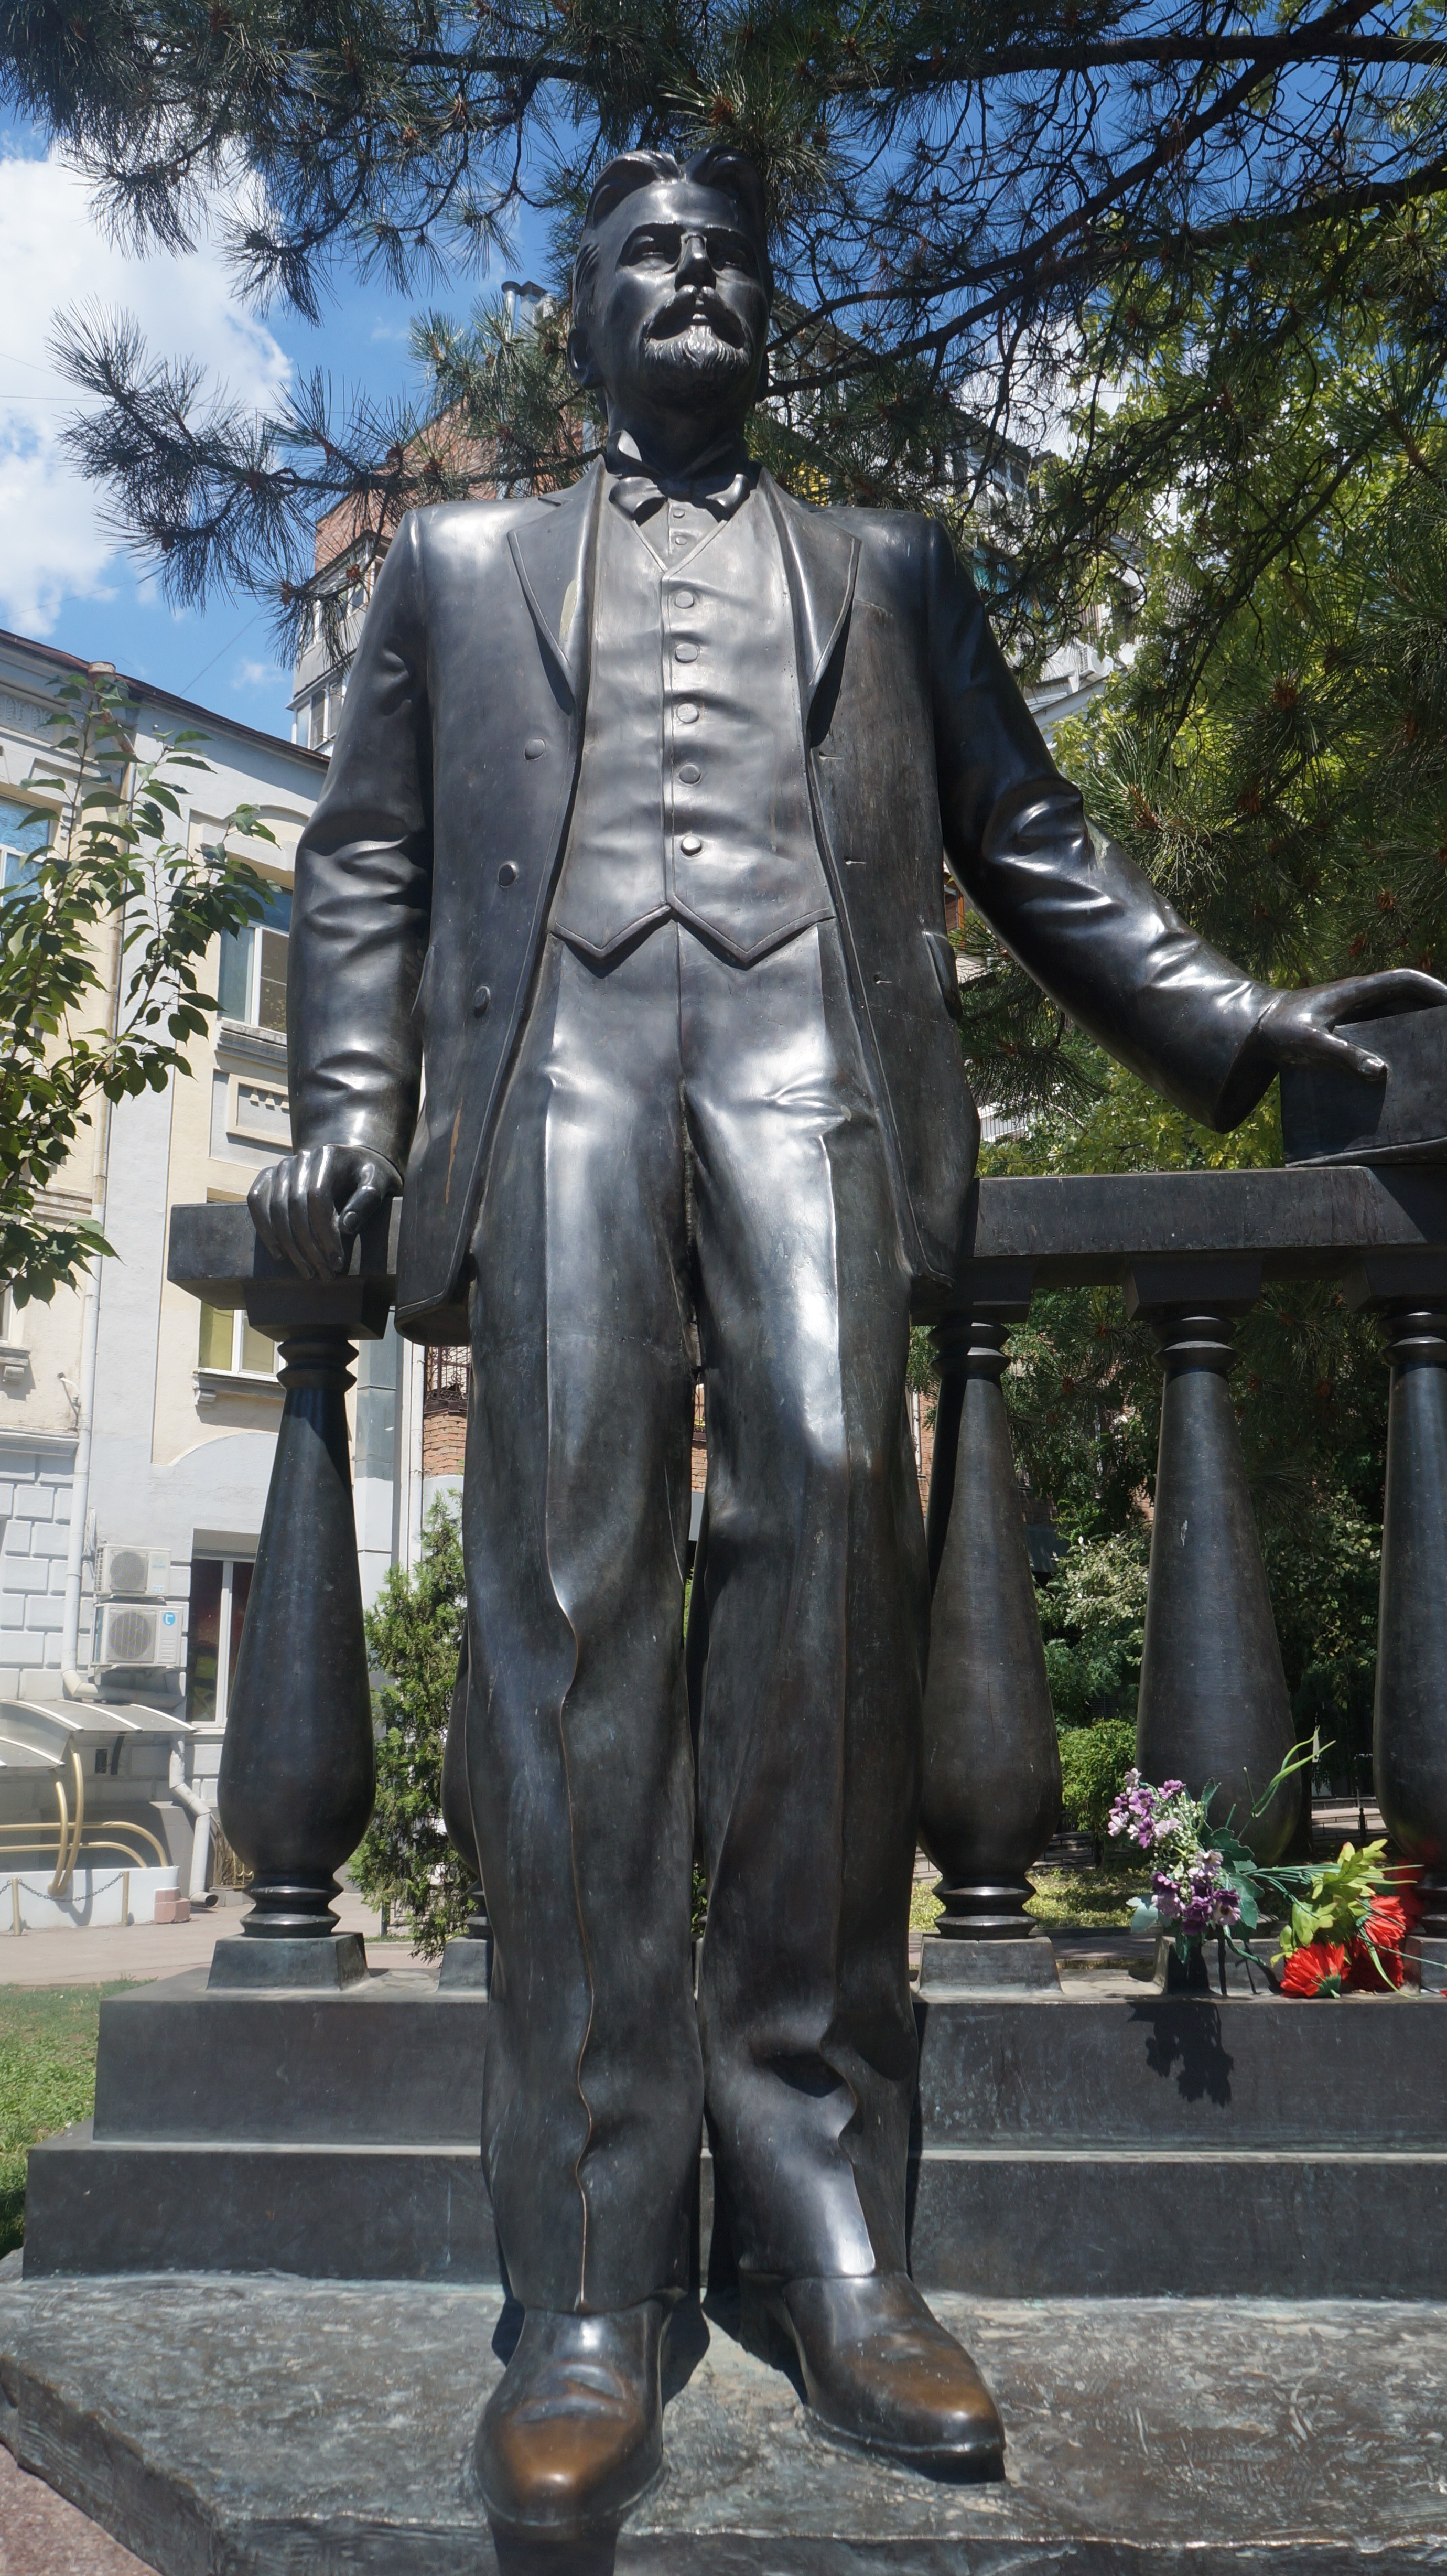
\includegraphics[width=100mm]{./imgs/rostov1.jpg}  
%  %\hfill
%\end{adjustwidth}
%  \caption{Estátua do escritor e dramaturgo Anton Tchékhov (1860--1904) em Rostov"-sobre"-o"-Don.}%

%\thispagestyle{empty}%

%\end{figure}
%\end{vplace}%

%\end{absolutelynopagebreak}

%\clearpage{\pagestyle{empty}\cleardoublepage}
%\makeatletter\@openrightfalse
\movetooddpage
\addcontentsline{toc}{part}{Rostov-sobre-o-Don [km 2807]}
\part*{ROSTOV-SOBRE-O-DON -- KM 2807\\\medskip\small{{[}AO SUL DE MOSCOU; A SUDOESTE DE\\NÍJNI NOVGOROD, KAZAN, SARANSK,\\\vspace{-4pt}SAMARA E VOLGOGRADO (STALINGRADO){]}}}


\chapter*{Vladímir Maiakóvski, a revolução que atira contra o (próprio) peito}
\addcontentsline{toc}{chapter}{[06/07/18] Vladímir Maiakóvski, a revolução que atira contra o (próprio) peito}
%\@openrighttrue\makeatother

\begin{flushright}
\emph{Rostov"-sobre"-o"-Don, 06 de julho de 2018}
\end{flushright}

Com traduções e ensaios de Augusto e Haroldo de Campos e Boris
Schnaiderman, o livro \emph{Poemas} nos traz uma antologia da obra do
russo Vladímir Maiakóvski como um panorama pré e pós"-revolucionário de
sua poesia\footnote{Vladímir Maiakóvski, \emph{Poemas.} Tradução de
  Augusto e Haroldo de Campos e Boris Schnaiderman. São Paulo:
  Perspectiva, 2017.}.

Para Boris Schnaiderman, no ensaio ``Maiakóvski: evolução e unidade'',

\begin{quote}
a evolução de formas e as mudanças de visada são apenas múltiplos
aspectos da mesma realidade poética.~O Maiakóvski~futurista
{[}pré"-revolucionário{]}, que usava blusa amarela, é o mesmo poeta da
Revolução {[}de 1917{]}, consciente e desafiador, assim como os poemas
que escreveu nas vésperas da morte {[}Maiakóvski se suicidou com um tiro
no peito{]} trazem a marca dos mesmos procedimentos poéticos, altamente
elaborados, que pôs em prática a partir de 1912\footnote{Idem, p. 32.}.
\end{quote}

O livro tem início com o poema ``A Vladímir Maiakóvski'', de autoria da
poeta Marina Tzvietaieva, para quem

\begin{verse}
\small{
Ele é dois: a lei e a exceção,\\
Ele é dois: cavalo e cavaleiro}\footnote{Idem, p. 21.}.
\end{verse}

Se, para a criação da arte revolucionária, forma e conteúdo
\emph{politicamente} revolucionários também precisam ser
\emph{artisticamente} radicais, o poeta da revolução e o poeta
revolucionário têm que se fundir em uma única e mesma pessoa. Para
Tzvietaieva, essas duas entidades encontraram"-se apenas uma vez no
centauro Maiakóvski -- ``Ele é dois: cavalo e cavaleiro'' --, ``pois ele
é um revolucionário poeta, o milagre de nossos dias''\footnote{Ibidem.}.

É assim que, ``De rua em rua'', o eu"-lírico iconoclasta e fortemente
imagético de Maiakóvski anseia que os ``Cisnes de pescoços"-campanários''
das catedrais se torçam (e/ou se asfixiem) ``nos fios do
telégrafo''\footnote{Idem, p. 96.}.

Desde o título"-desafio ``Algum dia você poderia?'', o poeta nos intima a
ler e auscultar, entre as

\begin{verse}
\small{
escamas de um peixe de estanho,\\
lábios novos chamando}\footnote{Idem, p. 100.}.
\end{verse}

E quando é que depararíamos com ``Algo em {[}São{]} Petersburgo'' como
``mamilos de granito'' (intumescidos, poeta?) ou ``o camelo de duas
corcovas do rio Neva''\footnote{Idem, p. 103.} sem a mediação de
Maiakóvski?

O olhar do eu"-lírico parece extrair e embaralhar a ontologia das coisas
de modo a transmutá"-la(s) com a alquimia de seus poemas"-experimento.
Assim, como se o poeta capturasse a nervura do mundo com uma câmera na
mão -- vale lembrar que o polivalente Maiakóvski também escreveu
roteiros para filmes --, o enquadramento de seu olhar, ``No automóvel''
em movimento, nos revela que

\begin{verse}
\small{
A cidade desatarrachou de súbito.\\
Os anúncios boquiabriam"-se de susto}\footnote{Idem, p. 112.}.
\end{verse}

Maiakóvski nos incita a resgatar nosso coração da ``jaula do
tórax''\footnote{Idem, p. 158.} (``Jubileu'') -- o carcereiro será
hipnotizado por versos entoados pela ``flauta de minhas próprias
vértebras''\footnote{Idem, p. 118.} (``A flauta"-vértebra'').

Em meio à carnificina da Primeira Guerra Mundial, Maiakóvski dá uma
forte bofetada no público burguês do cabaré artístico ``O cão vadio'' ao
recitar/disparar um de seus mais virulentos poemas"-desafio -- ``A
vocês!'':

\begin{verse}
\small{
Sabem vocês, inúteis, diletantes\\
Que só pensam encher a pança e o cofre,\\
Que talvez uma bomba neste instante\\
Arranca as pernas ao tenente Pietrov?}\ldots{}\footnote{Idem, p. 121.}
\end{verse}

Boris Schnaiderman nos conta que

\begin{quote}
aquela bofetada no público burguês, ao qual se lembrava a imoralidade de
sua vida boêmia, no momento em que o soldado russo morria nas frentes de
combate, provocou indignação geral entre os frequentadores do cabaré.
``O cão vadio'' por pouco não foi fechado, por causa daquela noite de
poesia\footnote{Idem, p. 36.}.
\end{quote}

A profunda irradiação de Maiakóvski pelo imaginário de sua época fez com
que, em meio à Revolução de Outubro, os marinheiros que investiam contra
o palácio de inverno do tsar, em São Petersburgo, cantassem os versos do
poema de luta ``Come ananás'':

\begin{verse}
\small{
Come ananás, mastiga perdiz.\\
Teu dia está prestes, burguês}\footnote{Idem, p. 135.}.
\end{verse}

Entretanto, o forte apelo político da obra de Maiakóvski -- uma obra que
entretecia as esferas subjetiva e histórica -- não a converteu em um
mero panfleto. Em contraposição aos burocratas partidários que
consideravam sua poesia hermética e elitista, Maiakóvski se apropria da
crítica limitada e a ressignifica em um poema ``Incompreensível para as
Massas'':

\begin{verse}
\small{
Chega\\
\hspace{40pt}de chuchotar\\
\hspace{100pt}versos para os pobres.\\
A classe condutora,\\
\hspace{83pt}também ela pode\\
compreender a arte.\\[5pt]
Logo:\\
\hspace{15pt}que se eleve\\
\hspace{60pt}a cultura do povo!\\
Uma só,\\
\hspace{30pt}para todos.\\
O livro bom\\
\hspace{60pt}é claro\\
\hspace{100pt}e necessário\\
a mim,\\
\hspace{55pt}a vocês,\\
\hspace{110pt}ao camponês}\footnote{Idem, p. 206.}.
\end{verse}

Em uma época que levou artistas a declinar da autoria de suas obras -- o
ímpeto revolucionário teria parido a miríade de criações --, o suicídio
de Maiakóvski, em 1930, aos 36 anos, também pode ser compreendido à luz
do autoritarismo contrarrevolucionário da União Soviética sob o punho de
Stálin. Afinal, em um poema premonitório de 1926 em homenagem ao poeta
Sierguéi Iessiênin, que se suicidara, Maiakóvski sentencia:

\begin{verse}
\small{
É preciso\\
\hspace{45pt}arrancar alegria\\
\hspace{120pt}ao futuro.\\
Nesta vida\\
\hspace{55pt}morrer não é difícil.\\
O difícil\\
\hspace{55pt}é a vida e seu ofício}\footnote{Idem, p. 187. Este escrito compôs o meu
  texto ``Maiakóvski, revolução, poesia e um tiro no peito'', publicado
  em 18/11/17 no caderno literário ``Aliás'', do jornal \emph{O Estado
  de S. Paulo}.}.
\end{verse}

\chapter*{Maturidade do adulto: recuperar a seriedade da criança ao brincar}
\addcontentsline{toc}{chapter}{[07/07/18] Maturidade do adulto: recuperar a seriedade da criança ao brincar}

\begin{flushright}
\emph{Rostov"-sobre"-o"-Don, 07 de julho de 2018}
\end{flushright}

Na confluência da avenida Budionovski com a rua Turguenievskaya, chego
ao Mercado Central de Rostov, a 5 quadras (se tanto) do rio Don.

Assim que começo a caminhar pela feira à russa, uma {\MinionPro{бабушка}}
(\emph{babuchka}, vovó) espirituosa e rechonchuda, com um lenço
multicolorido ao redor da cabeça e amarrado sob o queixo, me pega pela
mão e começa a conduzir este forasteiro por entre as barracas.

A \emph{babuchka} Alióna Ivánovna tem olhinhos vivazes porém pequeninos
-- o acúmulo de pele bem enrugada e flácida ilha seus olhos e os
transforma em pequenas frestas. Os cabelos brancos como fios de nuvem se
esgueiram por sob o lenço e lhe caem pelas têmporas e sobre a testa.
Quando a vovó sorri, o sol de verão reluz em sua coleção de dentes de
ouro -- na finada União Soviética, problemas dentários tendiam a
implicar a extração dos dentes e sua reposição por próteses de ouro,
como se a pátria do socialismo quisesse desdenhar do nobre metal burguês
colocando"-o na boca de seus banguelas proletários.

A \emph{babuchka} logo me faz aterrissar em cada uma das barracas.

Ela me leva a cheirar e a provar a policromia russa de legumes e
temperos, frutas e doces -- cada degustação pressupõe o toque, e as
pontas dos meus dedos vão se embebendo de sumo, óleo e açúcar.

Alióna Ivánovna alisa os pêssegos como se estivesse penteando o dorso de
um gato.

A vovó coloca um pêssego ao lado de uma maçã: ambos têm o mesmo tamanho
e as mesmas cores, com a predominância do amarelo, no pêssego, e do
vermelho, na maçã, como se o primeiro fosse a meia virada do avesso da
segunda.

Ao comparar a solidão de uma cereja bem vermelha com o bloco de carnaval
de um cacho de uvas graúdas, a \emph{babuchka} sentencia que a expressão
``cereja do bolo'' mais parece um prêmio de consolação para a fruta mais
triste que existe.

Para Alióna Ivánovna, a capa verde ao redor da espiga é o terno do
milho.

E quando a vovó me faz mergulhar as mãos numa bacia de amoras para
esmagá"-las como a argila malemolente das aulas de Educação Artística com
as professoras Cleide e Regina, lá pelos idos de 1988?

Tomates embebidos num molho de repolho, salsinha e orégano; pepinos e
picles recheados com berinjela e cenoura bem raladinha; beterrabas
amorfas e quase pretas de tão roxas ao lado de batatas pálidas e cabeças
de alho solenes que mais parecem os bulbos das igrejas ortodoxas.

Súbito, Alióna Ivánovna aponta com o dedo todo curvado pelo reumatismo
-- é como se o indicador direito da \emph{babuchka} tivesse uma corcova
-- para uma barraca com várias garrafas de plástico repletas de um
líquido bem dourado.

-- Se eu lhe dissesse que aquele óleo de girassol é o mais puro mel,
jovem, você não acabaria comprando gato por lebre?

Mal tenho tempo de sorrir, uma vez que a vovó já abriu a tampa de um
pote de açafrão com um cheiro ao mesmo tempo incisivo e apaziguador. Ela
me pergunta, então, de forma inusitada, se eu já estive no Saara. Por um
acaso, há pouco mais de 6 meses, eu singrei o Saara egípcio, nas
imediações da Cidade do Cairo, a bordo de um camelo.

-- Então me diga, jovem, se você não consegue imaginar um deserto de
dunas e mais dunas desse açafrão amarelo e denso, como se ele fosse o
irmão do meio entre a areia e a terra?

Quando faço menção de perguntar para a vovó Ivánovna se ela já %Alióna
pensou em escrever poesias com seu panteísmo colorido e sinestésico, ela
despeja uma profusão de sementes e amendoins em minhas mãos
emergencialmente abertas em concha.

-- Eu já trabalho neste mercado há mais de 50 anos, jovem. Para você,
que passa por aqui como um nômade, há apenas dois ou três tons de
marrom. Mas eu sei dizer se o amendoim está fresco ou não pela
intensidade de sua cor e pela textura de sua casca; quanto às sementes,
se elas não resistirem ao teste de uma leve dentada -- a \emph{babuchka}
posiciona uma semente entre os caninos e lhe impõe certa pressão --, é
preciso devolver ao útero da terra os rebentos que não conseguiram
vingar.

Chega a hora do batalhão de nabos e rabanetes. De tão bojudos, alguns
deles mais parecem chocalhos, e Alióna Ivánovna não se furta em
chacoalhá"-los, ritmicamente, como se fosse percussionista da banda
caribenha \emph{Las babuchkas de Rostov. }

Em seguida, em meio à mistura tresloucada de alhos com bugalhos,
despontam as tâmaras. Antes de ir a Israel, eu nunca provara uma tâmara,
essa verdadeira cápsula de açúcar, iguaria que me parece um bombom do
deserto. Contra o meu deleite, no entanto, a \emph{babuchka} sentencia
que o corpo abaulado (e como que pisoteado) da tâmara lhe dá a forma de
uma barata.

E que dizer dos limões russos radicalmente amarelos que mais parecem
filhotes do Sol? (Danada e casamenteira como ela só, Alióna Ivánovna me
sussurra que os bicos dos limões parecem tão intumescidos quanto os
mamilos da bela feirante -- de cabelos bem pretos e lisos como a crina
de um cavalo -- que não tira os olhos de mim desde que eu cheguei à
barraca.)

Quando chega a hora e a vez dos doces multicoloridos, eu pareço ouvir a
pergunta do palhaço de minha infância:

-- E hoje tem marmelada?

-- Tem, sim, senhor! -- exclama Alióna Ivánovna já munida de um saco de
marmeladas quadriculadas com todas as cores do arco"-íris.

Biscoitinhos com geleia; roscas e bombas de chocolate; tortas de nata;
pastéis, entre delgados e bojudos, com creme de limão; bolachas secas,
crispadas de açúcar, e bolachas com recheio de avelã; bolachas amorfas
que, mesmo no verão calorento de Rostov, parecem polvilhadas com a neve
russa; doces compactos como tijolos e de nomes impronunciáveis --
verdadeiros queijos de açúcar.

Quando a \emph{babuchka} me oferece um \emph{cherbet}, eu me sinto em
casa.

\textsc{alióna ivánovna:} Você já tinha provado o \emph{cherbet}?

\textsc{eu:} Em Novosibirsk, \emph{babuchka}, ele não é tão doce como o
daqui.

Rostov"-sobre"-o"-Don fica a mil quilômetros ao sul de Moscou, onde o
\emph{Diário de um escritor na Rússia} começou a ser escrito. Como um
tapete voador, o \emph{cherbet} me leva de volta ao Mercado Central de
Novosibirsk, capital da Sibéria Ocidental, cidade que fica a mais de 3
mil km a leste do Mercado Central de Rostov"-sobre"-o"-Don.

Conto para a \emph{babuchka} de Rostov que, há pouco menos de 1 ano, em
agosto de 2017, uma \emph{babuchka} de Novosibirsk, também com os
cabelos bem brancos (só que envoltos por um lenço vermelho), me ofereceu
o \emph{cherbet}, uma espécie de alfajor feito com frutas secas moídas e
sementes de girassol, nozes, mel e gergelim.

Enquanto conversamos, os olhos da senhora Olga Titova (a \emph{babuchka}
de Novosibirsk) vão ficando marejados. Quando lhe pergunto se está tudo
bem, ela saca do bolso do avental um pequeno porta"-retrato dourado com
uma foto de um jovem fardado -- um rapaz de olhos estreitos e lábios
finos, testa ampla e nariz grande e vigoroso.

-- Este é Oleg, meu marido: ele se parece com você.

-- E onde ele está agora, dona Olga?

Ela aperta minhas mãos antes de dizer que o soldado Oleg Tchernov foi um
dos 20 milhões de soviéticos ceifados pela Segunda Guerra Mundial.

-- Vá ao Museu Ferroviário de Novosibirsk -- faça isso por mim. Lá você
vai ver o vagão"-hospital onde meu Oleg morreu -- ele não suportou a
amputação de uma perna sem anestesia. {\MinionPro{Боже мой!}} (\emph{Boje mói!} Meu
Deus!)

Ao se despedir, a senhora Titova afaga meu rosto e, em seguida, me dá um
\emph{cherbet}.

-- Este é o doce favorito do Oleg -- ele vai ficar contente com o
presente. {\MinionPro{До свидaния!}} (\emph{Do svidania!} Até mais ver!)

Logo em seguida, vou até o Museu Ferroviário de Novosibirsk e encontro o
vagão"-hospital.

Quem caminha pelo vagão silencioso, entre as macas e os instrumentos
médicos perfilados, precisa se esforçar para imaginar que as cirurgias
traumáticas aqui realizadas implicavam a vida e a morte imediatas dos
soldados mutilados após o inferno do \emph{front}. Com sorte, doses
minguadas de vodca anestesiavam as amputações -- no mais, salve"-se quem
puder!

E eis que os médicos, enfermeiras e moribundos do vagão"-hospital
transpassado por agonia e sangue eram vigiados por retratos do líder
soviético Ióssif Stálin, mentor de julgamentos políticos que resultaram
em milhões de execuções e expurgos para campos de trabalho forçado
espraiados pelos confins da Sibéria.

Sem ter como tranquilizar os soldados trêmulos antes das amputações com
serras, facas e machados, as enfermeiras só faziam apelar ao terror e à
devoção que Stálin inspirava para (tentar) aplacar os gritos e uivos:

-- Aguente firme, vamos! Porte"-se bem, soldado: Stálin está vendo você!

A \emph{babuchka} Alióna Ivánovna fica com os olhinhos marejados -- as
frestas se transformam em pequenos lagos -- ao ouvir a história de Olga
Titova e Oleg Tchernov. (A vovó não me diz nada, mas é bem possível que
ela mesma, como ocorre na maioria das famílias russas, tenha perdido
alguém em meio à guerra.)

Para resgatá"-la da tristeza e da saudade incontornáveis, eu me lembro de
uma segunda história siberiana -- dessa vez, proveniente das imediações
da aldeia de Listvianka, que fica a mais de 1.900 km a leste de
Novosibirsk, onde estive pouco menos de duas semanas antes de chegar ao
mercado em que acabei conhecendo a senhora Olga Titova.

Peço à \emph{babuchka} Alióna Ivánovna que me acompanhe em minha
narrativa a bordo do Grande Expresso Transiberiano.

Da janela da minha cabine no trem, vejo a sucessão vertiginosa de
estepes entremeadas pela taiga, a floresta siberiana de coníferas que
mais parece um pelotão perfilado. Logo desponta uma casinha rústica de
madeira, em frente da qual um velho de cabelos e barbas bem brancos
parte a lenha e limpa o suor do rosto com um lenço amarelo amarrado ao
redor do punho. E eis que a jovem Nástia, a funcionária do trem que
cuida das cabines, nota que não consigo tirar os olhos da sucessão
infinda das estepes. Ela pede, então, que eu imagine a vastidão
siberiana recoberta de neve no ápice do inverno. Quando faço menção de
ficar boquiaberto, Nástia saca uma garrafa de vodca de não sei onde e me
diz:

-- Para nós, os russos siberianos, 40 quilômetros, 40 graus abaixo de
zero e 40\% de teor alcoólico não são nada -- absolutamente nada!

Nástia enche dois copinhos e, antes de decretar que precisamos
entorná"-los em um só trago, ela sentencia:

-- {\MinionPro{На здоровье!}} (\emph{Na zdorovie,} saúde!)

Súbito, o Grande Expresso Transiberiano passa a margear o lago Baikal, e
Nástia me revela, entre tragos e soluços, que ``o Baikal é o mais antigo
e profundo lago da Terra, com 25 milhões de anos e 1680 metros de
profundidade. Há quem diga que o Baikal é um oceano nascente, já que
suas margens crescem 2 centímetros por ano''. (Nástia me mostra as unhas
e as pontas dos cabelos como parâmetros para a expansão do gigante
Baikal.)

Descemos do trem e vamos até as margens. Eis que vejo a pequena Sacha a
olhar, sucessivamente, de sua bailarina que dança impulsionada por uma
manivela para o vaivém das marolas do Baikal. Súbito, Sacha pergunta
para a mãe:

-- Quando acaba a corda, a bailarina para de dançar, né, mamãe?

-- É isso mesmo, querida.

Sacha volta a olhar para as marolas do Baikal. Súbito, ela pergunta:

-- E quando vai acabar a corda do lago, mamãe?\footnote{Parte deste
  escrito compôs o meu texto ``Rússia: Uma volta ao passado'', publicado
  em 30/09/17 no caderno literário ``Aliás'', do jornal \emph{O Estado
  de S. Paulo}.}

\clearpage{\pagestyle{empty}\cleardoublepage}
\movetooddpage
\addcontentsline{toc}{part}{A bordo do trem que vai de Rostov-sobre-o-Don a Sotchi}
\part*{A BORDO DO TREM QUE VAI DE ROSTOV-SOBRE-O-DON A SOTCHI}

\chapter*{Boris Pasternak pergunta à história: Pode o coração ser uma célula revolucionária?}
\addcontentsline{toc}{chapter}{[08/07/18] Boris Pasternak pergunta à história: Pode o coração ser uma célula revolucionária?}

\begin{flushright}
\emph{Entre Rostov"-sobre"-o"-Don e\\Sotchi, 08 de julho de 2018}
%\emph{A bordo do trem que vai de Rostov"-sobre"-o"-Don\\a Sotchi, 08 de julho de 2018}
\end{flushright}

Ourives da palavra e escultor de imagens poéticas em meio à prosa, o
escritor russo Boris Pasternak ressoa em sua obra"-prima \emph{Doutor
Jivago} a máxima dostoievskiana segundo a qual a beleza salvará o mundo.
Munido de um profundo panteísmo, Pasternak celebra o encantamento diante
da natureza como a crisálida das metáforas. Assim, o narrador/eu"-lírico
de \emph{Doutor Jivago} recita que ``observar o rio fazia doer os olhos.
As águas ondulavam e refletiam a luz do sol como folhas de metal''. O
lago, por sua vez, ``estava repleto de nenúfares. O barco cortou essa
massa vegetal com um barulho seco. A água surgia no meio da folhagem
aquática como o suco no triângulo talhado da melancia''\footnote{Boris
  Pasternak, \emph{Doutor Jivago.} Tradução de Sônia Branco. São Paulo:
  Companhia das Letras, p. 17; p. 25.}.

E que dizer da precocidade poética do menino Iúri Jivago, quando ele
sente que ``o odor do carvão usado para ferver o samovar'' abafa ``o
cheiro de tabaco e o perfume dos girassóis'' enquanto o chá é servido?
Estamos diante do mesmo ímpeto sinestésico que descobre ``um odor
adstringente de nozes frescas em cascas verdes ainda macias, que
escurecem ao menor toque'', sinestesia que entrevê a paralisia dos
flocos de neve no ar, flocos que descem tão lentamente ``como o miolo do
pão atirado na água para alimentar os peixes''\footnote{Idem, p. 15; p.
  69; p. 238.}.

Se a ourivesaria poética de \emph{Doutor Jivago} exalta, em cada uma de
suas linhas/versos, a beleza que salvará o mundo, precisamos descobrir
se o mundo -- isto é, a história com a qual o romance se funde e se
confunde -- conseguirá salvar a beleza.

Desde a mais tenra infância até seus últimos momentos em um bonde
moscovita; desde que se reconhece como poeta e começa a amar a bela e
intensa Larissa Fiódorovna com todas as fímbrias de seu lirismo, a vida
de Iúri Jivago se vê afetada pelos grandes eventos históricos que acabam
por plasmar o transcurso ulterior da Rússia e do século \versal{XX}: a tentativa
revolucionária de derrubar a monarquia tsarista em 1905; a Primeira
Guerra Mundial; a queda do tsar, em fevereiro de 1917, e a tomada do
poder pelos bolcheviques capitaneados por Vladímir Lênin, oito meses
depois; a encarniçada guerra civil que contrapõe os russos vermelhos e
revolucionários aos russos brancos, constituídos por um amálgama
sumamente heterogêneo de partidários do tsar e defensores do governo
constitucional instaurado em fevereiro de 1917, tropas inglesas e
francesas, tchecas e polonesas, estadunidenses e japonesas; a
coletivização forçada das propriedades rurais, o saque e a pilhagem da
produção agrícola pelo governo revolucionário e a fome no campo; as
execuções de (supostos) contrarrevolucionários e sabotadores e os
expurgos para campos de trabalhos forçados sob a ditadura do líder
soviético Ióssif Stálin.

Em um momento de radical entrelaçamento entre vida e história, o médico
Iúri Jivago caminha -- ou, melhor, se esgueira -- pelas ruas de uma
Moscou transpassada pelas barricadas de vermelhos e brancos em meio à
guerra civil. Súbito (e como se fosse uma miragem), surge um jornaleiro
-- um menino de bochechas coradas sob uma boina surrada -- e lhe vende
uma

\begin{quote}
edição especial, impressa apenas de um lado da folha, que continha um
comunicado do governo de Petersburgo anunciando a criação do Conselho de
Comissários do Povo e a instauração na Rússia do poder soviético e da
ditadura do proletariado. A chuva açoitava"-lhe os olhos, e grãos
cinzentos de neve recobriam as linhas impressas do jornal. Mas não era
isso que atrapalhava a leitura. A grandiosidade e a eternidade daquele
instante o abalavam e o impediam de voltar a si. É a história. Acontece
uma vez na vida\footnote{Idem, p. 209.}.
\end{quote}

Ocorre que, com suas origens pequeno"-burguesas, Iúri Jivago e Larissa
Fiódorovna logo descobrem que o autoproclamado Éden do proletariado tem
outros planos para o destino de seu amor. Munida de baioneta, a história
cinde a comunhão de Larissa e Iúri com a crueldade de suas engrenagens.
Com a pecha de potenciais inimigos do povo e da revolução, Iúri e
Larissa se refugiam em um rincão gélido da Sibéria para escapar ao
fuzilamento sumário. Ora, é radicalmente sintomática a mensagem
subliminar de Pasternak: se o coração é uma célula revolucionária, que
utopia e que novo tempo histórico são esses que não conseguem acalentar
em seu seio a comunhão de um casal apaixonado?

A publicação de \emph{Doutor Jivago} em Milão, em 1957, transforma Boris
Pasternak em traidor da pátria soviética. Em meio às disputas
político"-culturais da Guerra Fria, Pasternak é coagido pelo governo da
\versal{URSS} a recusar o Nobel de Literatura com que a Academia Sueca o
agraciara em 1958, do contrário o escritor teria que abandonar o país
imediatamente. Ao fim e ao cabo, Pasternak só aceita o exílio interno em
Peredelkino, região próxima a Moscou, por não conceber a vida fora de
sua única e verdadeira pátria, a grande literatura russa\footnote{Este
  escrito compôs o meu texto ``Jivago, uma crítica aos rumos da
  revolução'', publicado em 06/01/18 no caderno literário ``Aliás'', do
  jornal \emph{O Estado de S. Paulo}.}.

%\pagebreak
\clearpage
\thispagestyle{empty}

\movetoevenpage
\begin{absolutelynopagebreak}
\begin{vplace}
\begin{figure}[H]
\begin{adjustwidth}{-1.8cm}{}
  %\centering
  \vspace{2.7cm}
  %\hspace{0.5cm}
  \includegraphics[width=130mm]{./imgs/sotchi2.jpg}  
  %\hfill
\end{adjustwidth}
  \caption{Datcha do ditador soviético Ióssif Stálin (1878-1953) em Sotchi, às margens do Mar Negro}%

\thispagestyle{empty}

\end{figure}
\end{vplace}

\end{absolutelynopagebreak}

%\movetoevenpage
%\begin{absolutelynopagebreak}
%\begin{vplace}
%\begin{figure}[H]
%\begin{adjustwidth}{-2.7cm}{}
%  %\centering
%  \vspace{-2.5cm}
%  \hspace{2.2cm}
%  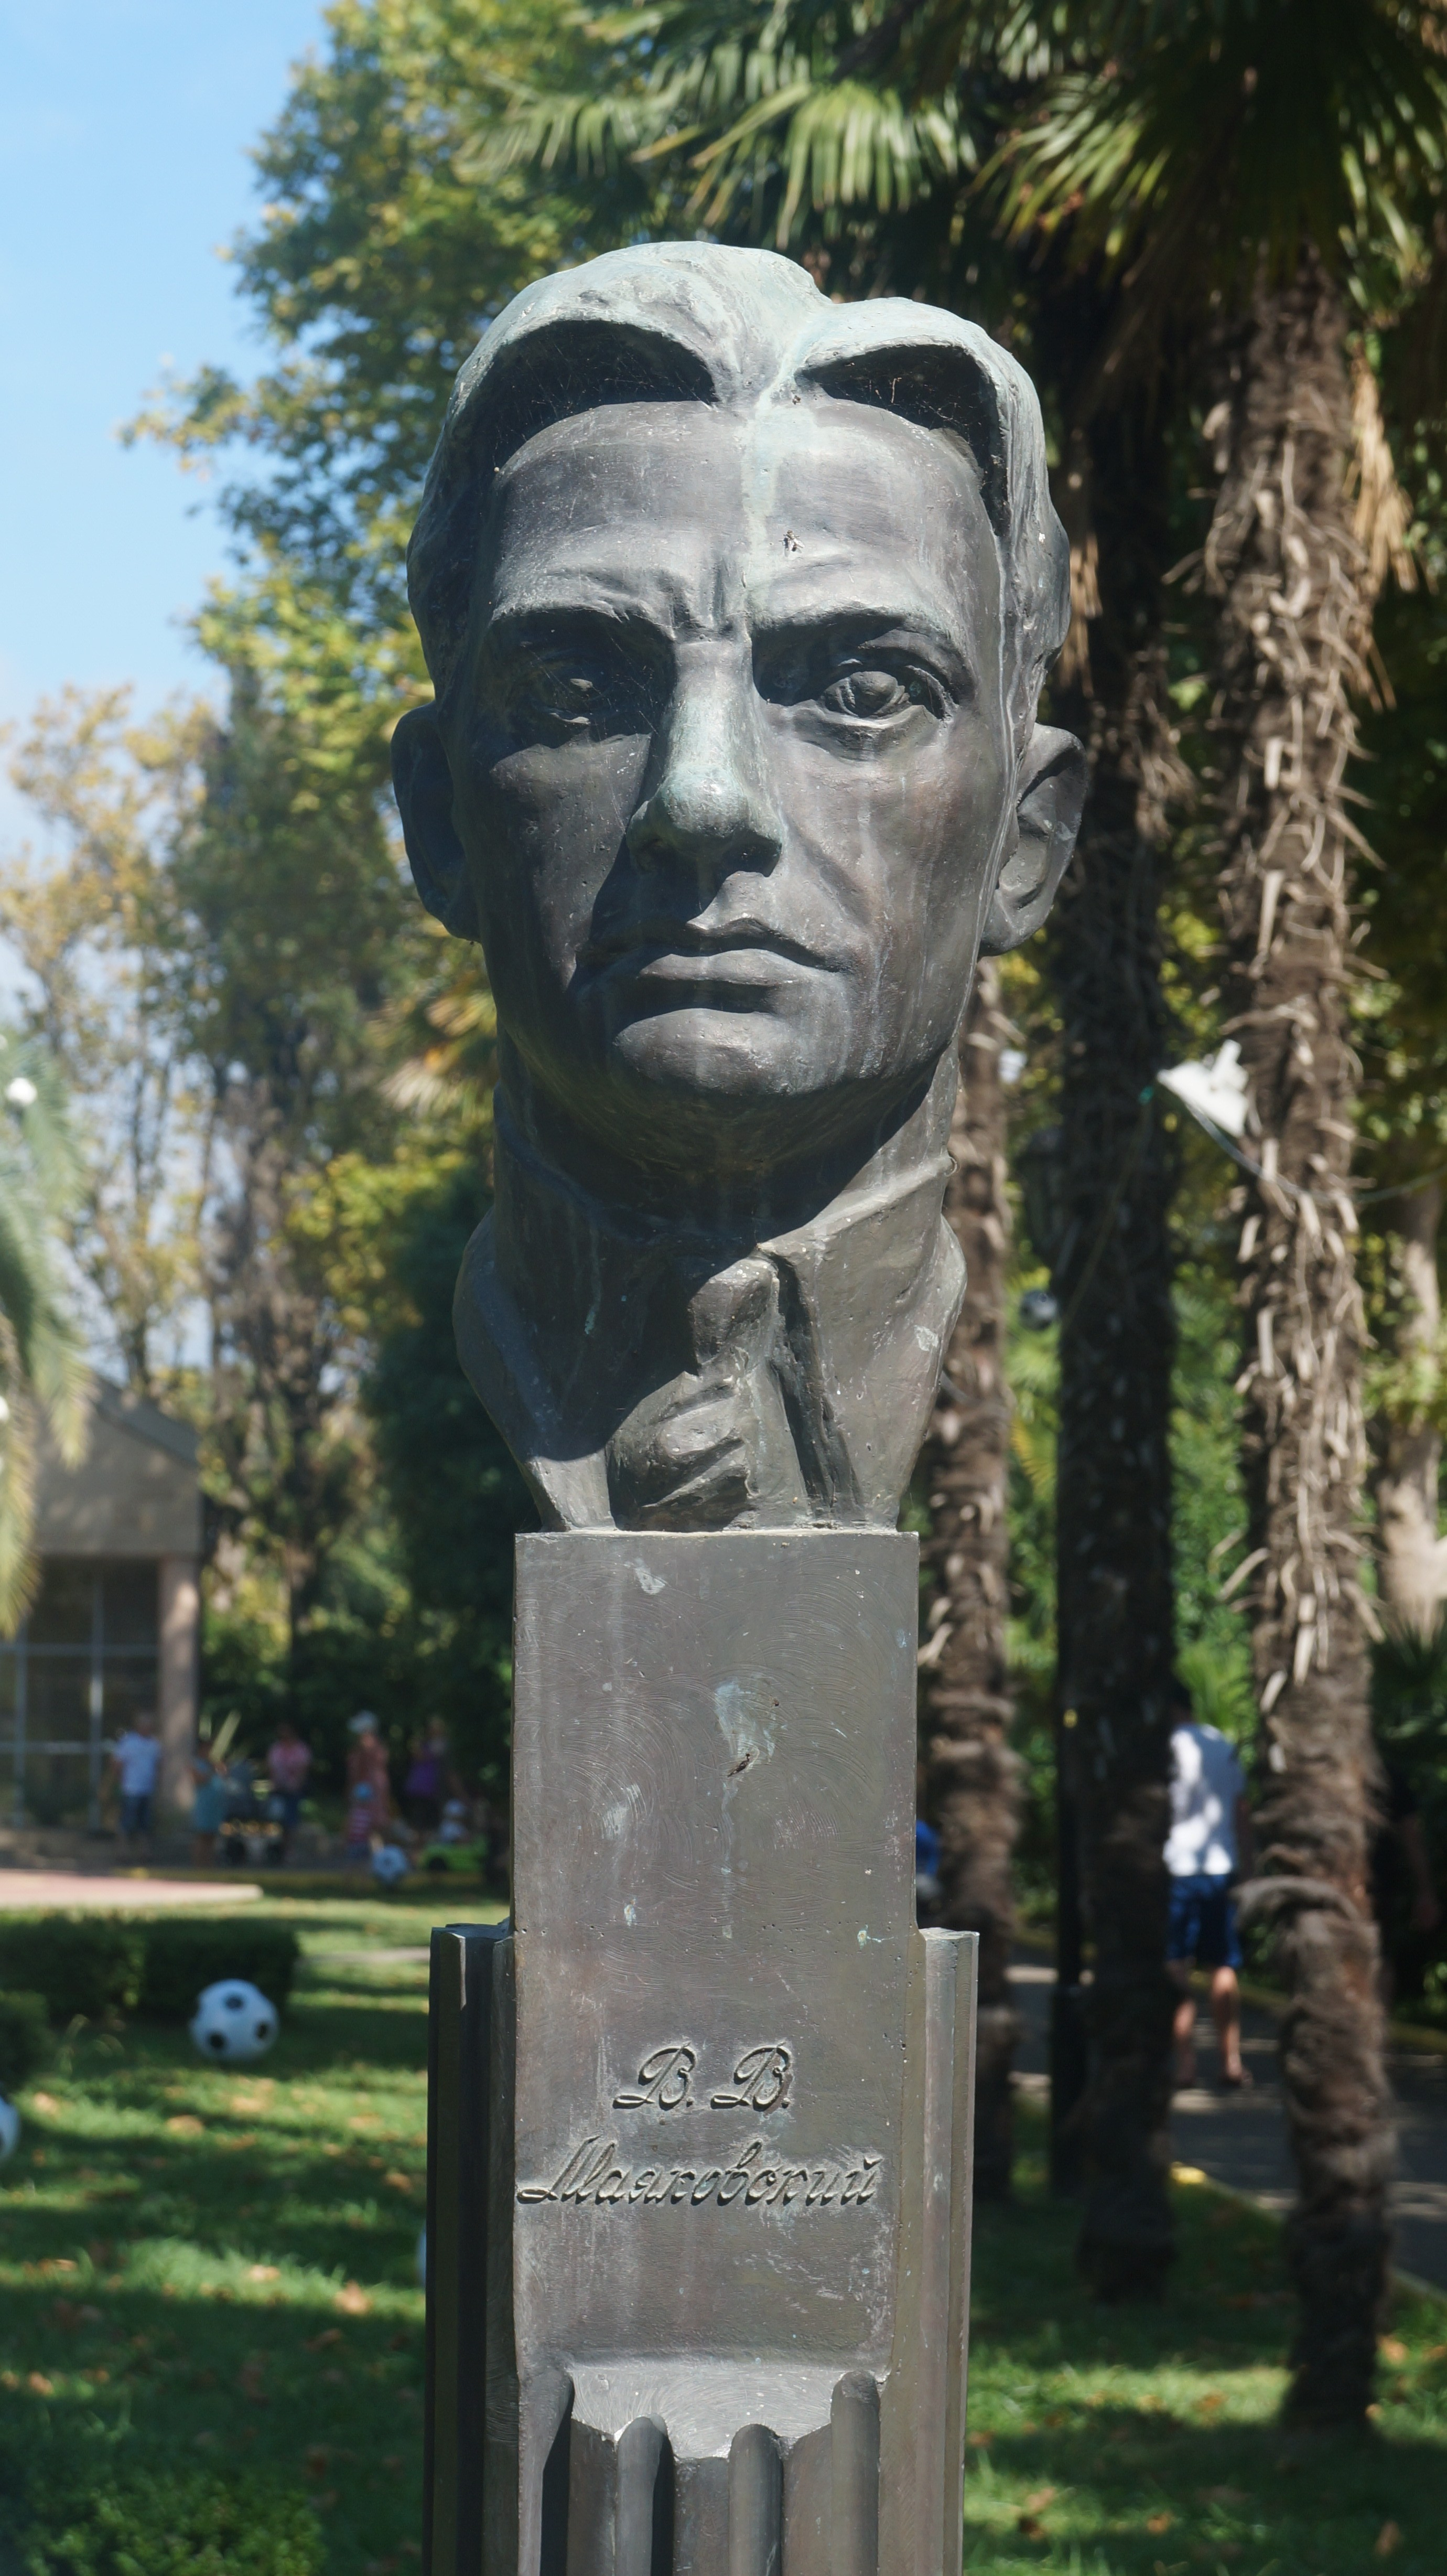
\includegraphics[width=100mm]{./imgs/sotchi1.jpg}  
%  %\hfill
%\end{adjustwidth}
%  \caption{Busto do poeta russo Vladímir Maiakóvski (1893--1930) em Sotchi, às margens do Mar Negro.}%

%\thispagestyle{empty}%

%\end{figure}
%\end{vplace}%

%\end{absolutelynopagebreak}

%\clearpage{\pagestyle{empty}\cleardoublepage}
%\makeatletter\@openrightfalse
\movetooddpage
\addcontentsline{toc}{part}{Sotchi [km 3353]}
\part*{SOTCHI -- KM 3353\\\medskip\small{{[}AO SUL DE MOSCOU E DE ROSTOV-SOBRE-O-DON;\\A SUDOESTE DE NÍJNI NOVGOROD, KAZAN, SARANSK,\\\vspace{-4pt}SAMARA E VOLGOGRADO (STALINGRADO){]}}}


\chapter*{Quando o cume prenuncia a vertigem da queda: Uruguai e Brasil; Napoleão, Hitler e Stálin}
\addcontentsline{toc}{chapter}{[09/07/18] Quando o cume prenuncia a vertigem da queda: Uruguai e Brasil; Napoleão, Hitler e Stálin}
%\@openrighttrue\makeatother

\begin{flushright}
\emph{Sotchi, 09 de julho de 2018}
\end{flushright}

Quem poderá negar que a participação em uma Copa do Mundo representa o
ápice da carreira de um jogador de futebol?

Ninguém deixaria de agarrar tal oportunidade com unhas e dentes.

Mas e quando o cume prenuncia a vertigem da queda?

Há três dias, em jogo válido pelas quartas de final da Copa do Mundo, o
Uruguai foi derrotado pela França, em Níjni Novgorod, por 2 a 0.

No mesmo dia, só que em Samara, o Brasil foi derrotado pela Bélgica, por
2 a 1, em jogo também válido pelas quartas do Mundial.

Além de estarmos diante da eliminação de dois campeões mundiais
sul"-americanos por equipes europeias, as quedas de Uruguai e Brasil
envolvem outra confluência -- mais tensa e essencial: os gols que, ao
fim e ao cabo, foram decisivos para o desenlace das partidas decorreram
de falhas de jogadores dos próprios times eliminados.

Já no segundo tempo, o Uruguai perdia por 1 a 0, mas, ainda assim,
procurava agredir a França com raça. O 1 a 1 teria levado o jogo para a
prorrogação ou mesmo para os pênaltis.

O gol brasileiro parecia maduro já antes dos 20 minutos do primeiro
tempo, tamanha a voracidade com que atacávamos os belgas.

Aos 15 minutos do segundo tempo, o francês Griezmann disparou um chute
perfeitamente defensável de fora da área, mas o goleiro uruguaio
Muslera, como se tivesse mãos de alface, engoliu um frango clamoroso.

Aos 8 minutos do primeiro tempo, o zagueiro Thiago Silva enfiou uma bola
na trave belga (bola na trave não altera o placar); 5 minutos depois, no
entanto, após escanteio venenoso cobrado pelo belga Chadli, Kompany
desviou a bola no primeiro pau; na sequência, a pelota bateu no braço do
meia brasileiro Fernandinho e, por um baita golpe de azar, foi morrer no
fundo das redes da nossa seleção. Gol contra.

Autor de \emph{Massa e poder}, o escritor judeu de origem búlgara Elias
Canetti\footnote{Elias Canetti, \emph{Massa e poder.} Tradução de Sérgio
  Tellaroli. São Paulo: Companhia das Letras, 1995.} bem poderia
sentenciar que a psicologia de massas é tão implacável quanto tangível:
o erro fatal do goleiro uruguaio se alastrou pelo desempenho pífio de
seus companheiros de time como uma epidemia. Após o frango, o jogo
acabou para o Uruguai.

O Brasil sentiu o gol precoce (e injusto) dos belgas (isto é, de
Fernandinho), mas continuou atacando o adversário. Até então, nossa
seleção jamais saíra perdendo no Mundial da Rússia -- tal fato, a
despeito da experiência dos jogadores, bem pode gerar ansiedade em uma
partida das quartas. Ocorre que, na sanha de empatar o marcador, o
Brasil comandado pelo conservador (isto é, retranqueiro) técnico Tite
cedeu contra"-ataques aos belgas. Num deles, aos 30 minutos do mesmo
primeiro tempo, a Bélgica abriu 2 a 0 num belo chute cruzado de fora da
área disparado por De Bruyne.

Como era de se esperar, o Brasil pressionou a Bélgica durante todo o
segundo tempo. Aos 30 minutos, Philippe Coutinho cruzou uma bola
açucarada para Renato Augusto, que, de cabeça e no cantinho, desviou dos
mais de 2 metros do goleirão belga Courtois: 2 a 1.

Cinco minutos depois, o mesmo Renato Augusto, frente a frente com um
Courtois já rendido, perdeu um gol feito da entrada da grande área -- se
não tivesse passado a 20 centímetros (se tanto) da trave adversária, a
bola rasteira e caprichosa teria empatado o jogo.

Sem o frango do goleiro Muslera, o Uruguai poderia ter empatado a
partida com a França; sem o frango do goleiro Muslera, o Uruguai poderia
ter virado a partida em cima da França; sem o frango do goleiro Muslera,
o Uruguai poderia ter eliminado a França e chegado à semifinal -- a taça
do tricampeonato mundial (1930; 1950; 2018) estaria a um triz das mãos
de Muslera, as mesmas mãos de alface que propiciaram o frango.

Sem a fatalidade do gol contra do meia Fernandinho, o Brasil não teria
saído atrás contra a Bélgica; sem a fatalidade do gol contra do meia
Fernandinho, o Brasil não teria se exposto aos contra"-ataques belgas e
tomado a pá de cal do segundo gol; sem a fatalidade do gol contra do
meia Fernandinho, o Brasil poderia ter eliminado a Bélgica e chegado à
semifinal -- a taça do hexacampeonato mundial (1958; 1962; 1970; 1994;
2002; 2018) estaria a um triz do braço direito de Fernandinho, o mesmo
braço que propiciou o gol contra.

Os milhões de euros (e/ou de liras) que Muslera ganha anualmente
defendendo a meta do Galatasaray, da Turquia, podem até dourar a pílula
do frango. Mas o caráter culposo do frango vai rondar o goleiro uruguaio
como um espectro doloso até o fim de sua carreira -- a bem dizer, até o
fim de seus dias. Muslera poderá ganhar todos os títulos imagináveis
daqui para diante -- a sucessão de taças tentará soterrar a latência da
memória. Mas, ainda que o Uruguai venha a se tornar tricampeão mundial
em 2022, no Catar, com Muslera à frente de sua meta, a Celeste já
poderia ser tetracampeã. (Assim insinuarão os olhares dúbios que
pairarão sobre Muslera a partir de agora; é isso que Muslera passará a
escutar, à revelia de todas as suas vitórias, quando se envolver em
discussões e brigas.)

Os milhões de libras esterlinas (e/ou de dólares) que Fernandinho ganha
anualmente jogando no meio"-campo do Manchester City, da Inglaterra,
podem até dourar a pílula do gol contra. Mas o caráter culposo do gol
contra vai rondar o meia brasileiro como um espectro doloso até o fim de
sua carreira -- a bem dizer, até o fim de seus dias. Fernandinho poderá
ganhar todos os títulos imagináveis daqui para diante -- a sucessão de
taças tentará soterrar a latência da memória. Mas, ainda que o Brasil
venha a se tornar hexacampeão mundial em 2022, no Catar, com Fernandinho
em nosso meio"-campo, a seleção Canarinho já poderia ser heptacampeã.
(Assim insinuarão os olhares dúbios que pairarão sobre Fernandinho a
partir de agora; é isso que Fernandinho passará a escutar, à revelia de
todas as suas vitórias, quando se envolver em discussões e brigas.)

Muslera e Fernadinho terão o apoio e o consolo mais do que devidos de
seus entes queridos, amigos verdadeiros e torcedores sinceros.

Muslera e Fernandinho jamais teriam cometido suas falhas se não tivessem
sido convocados para a Copa do Mundo da Rússia e se não tivessem
alcançado o auge de suas carreiras -- conquistas que jamais despontarão
para os ressentidos que, para aplacar a mais rematada inveja, só farão
criticá"-los a partir de agora.

Ninguém deixaria de agarrar a oportunidade de Muslera e Fernandinho com
unhas e dentes.

Ainda assim, o sumo infortúnio do goleiro uruguaio e do meia brasileiro
não nos pode mostrar o paradoxo do cume que prenuncia a vertigem da
queda?

A sina de Muslera e Fernandinho, no campo de futebol, lembra a sina do
generalíssimo Napoleão Bonaparte, no campo de batalha.

Consta que, após a derrota clamorosa para os russos -- decorrente da
invasão frustrada da Rússia pelas tropas francesas entre 1812 e 1814 --,
Napoleão Bonaparte não vê outra saída senão o suicídio.

O generalíssimo já galgara todos os postos e já pisara sobre todas as
cabeças.

Ainda assim, não foram as vitórias incontestáveis que desvelaram a
Napoleão a contingência e a fragilidade que aproximam o cume da queda.
Foi a derrota irredimível que, ao fim e ao cabo, revelou ao imperador
que a ascensão vertiginosa está umbilicalmente irmanada ao beco sem
saída daquele que já não pode mais cair sem ter que se ajoelhar.

O senhor se vê aguilhoado a seus escravos.

A genealogia de Bonaparte remonta à pequena nobreza córsega, isto é, ao
baixo clero do baixo clero da nobreza europeia. Assim, a ascensão
vertiginosa do então jovem segundo tenente aos quadros máximos \emph{de
la Patrie} após a Revolução Francesa também pode se relacionar,
sub"-repticiamente, a feridas e ressentimentos de classe que, quando
ardem em espíritos sedentos por poder e distinção, fustigam o dorso da
vontade para que ela alce voos sempre mais altos.

Nesse sentido, a vitória e a desforra finais só se consumariam quando
Napoleão tivesse varrido da Europa todo o alto clero da nobreza, em
especial o nobilíssimo Alexandre \versal{I}, Tsar de Todas as Rússias.

Nesse mesmo sentido, será que o cabo austríaco e conquistador da Europa
Adolf Hitler teria invadido a União Soviética se o segundo tenente
imperial Napoleão Bonaparte tivesse desbancado o tsar Alexandre \versal{I}?

Nesse mesmíssimo sentido, será que o filho de sapateiro georgiano e Tsar
do Partido Comunista de Todas as Rússias Ióssif Stálin teria expandido a
Cortina de Ferro até Berlim se Alexandre \versal{I} não tivesse levado suas
tropas até Paris após desbancar Napoleão?

\part{A BORDO DO AVIÃO QUE VAI DE SOTCHI A KALININGRADO (KÖNIGSBERG)}

\chapter*{Ser e não ser, eis a resposta (e a sentença) de Stálin}
\addcontentsline{toc}{chapter}{[10/07/18] Ser e não ser, eis a resposta (e a sentença) de Stálin}

\begin{flushright}
\emph{Entre Sotchi e Kaliningrado\\(Königsberg), 10 de julho de 2018}
%\emph{A bordo do voo que vai de Sotchi a Kaliningrado\\(Königsberg), 10 de julho de 2018}
\end{flushright}

Nas últimas 3 horas de viagem, o trem que me leva de Rostov"-sobre"-o"-Don
a Sotchi vai margeando as praias de areia escura e pedras polimorfas do
Mar Negro.

Por vezes, os gritos efusivos da criançada a se esbaldar na água
tensionam a cadência monocórdia do trem pelas infindáveis bitolas do
trilho.

Sem ser polvilhado por nuvens e de vez em quando singrado por gaivotas,
o céu de um azul claríssimo contrasta com as águas escuras e brilhantes
como o dorso de uma pantera.

Súbito, o Mar Negro caucasiano, outrora balneário dos líderes
soviéticos, me remete a uma colocação do argentino Jorge Luis Borges
sobre a luta de classes que o mar anima (e naufraga) em seu bojo.

Em sua imensidão somente comparável à virtual infinitude do horizonte, o
mar não poderia ser mais rico.

Em sua monotonia de formigueiro composta por marolas e marés sempre
idênticas e reiteradas, o mar não poderia ser mais pobre.

Do outro lado do trilho, uma vegetação densa e cerrada transforma o
Cáucaso na Mata Atlântica da minha adolescência que entremeava as
descidas para o litoral sul de São Paulo. (Só faltam as chaminés
fosforescentes de Cubatão e os caiçaras vivazes vendendo espetinhos de
siri.)

Mal chego a Sotchi e já me dirijo à \emph{datcha} (casa de veraneio) em
que o ditador Ióssif Stálin costumava passar os meses de agosto,
setembro e outubro.

Segundo o caucasiano Oleg, que trabalha na manutenção da \emph{datcha}
há mais de 15 anos, Stálin tinha à sua disposição 17 casas de veraneio,
mas o bolchevique só chegou a viver efetivamente em 5 delas: duas na
hoje República Autônoma da Abecásia, ao norte da Geórgia (uma delas, por
sinal, banhada pelo lago Ritsa); duas em Moscou; e (Oleg fala com
orgulho) ``esta \emph{datcha} aqui em Sotchi, a maior e mais bonita de
todas''.

Quem chega ao jardim frondoso da \emph{datcha} se vê circundado (ou,
melhor, enquadrado) por quatro arestas de uma casa de dois andares e tom
verde suave. É como se, através das numerosas janelas com entalhes de
madeira, Stálin quisesse entrever (e capturar) a chegada de quaisquer
visitantes/potenciais invasores.

Girassóis sumamente amarelos e convidativos -- será que Stálin
convenceu/coagiu o pintor holandês Vincent Van Gogh a se filiar ao
Partido Comunista? -- se veem entremeados por arbustos bem podados,
pequenas flores róseas e esbranquiçadas, com pétalas suaves a serem
levadas pela brisa, e árvores altivas e sem galhos, encimadas por folhas
longilíneas e pontiagudas como as lâminas de uma tesoura -- ou de um
punhal georgiano da juventude de Stálin, quando o bolchevique costumava
roubar (isto é, expropriar) bancos para a causa da revolução. {[}Consta
que, entre uma baforada e outra de seus onipresentes cachimbos, Stálin
deu boas risadas sob seu vasto bigode quando seus oniscientes canais de
(contra)espionagem o informaram de uma máxima forjada pelo poeta e
dramaturgo alemão Bertolt Brecht: ``O que é o crime de assaltar um banco
comparado com o crime de fundar um banco?''\footnote{Bertolt Brecht, ``A
  ópera de três vinténs''. In: \emph{Teatro completo.} Volume 3.
  Tradução de Wolfgang Bader e Marcos Roma Santa. São Paulo: Paz e
  Terra, 1992, p.~11.}.{]}

Diz Oleg que Stálin, como rematado caucasiano, gostava de caçar ursos
pelo amplo perímetro da \emph{datcha}. Ademais, o ditador apreciava
alimentar pequenos esquilos que deslizavam até a varanda traseira da
casa de veraneio pelos galhos de enormes árvores ali postadas como
sentinelas.

Quando entro na primeira ala da \emph{datcha}, deparo com um tapete
(persa?)~bem vermelho e repleto de ornamentos ladeado por paredes
revestidas de madeira (e forradas de escutas?). Acarpetada, a escada
conduzida por um corrimão bojudo desemboca em uma sala de
jantar/reuniões ao centro da qual se posta uma mesa retangular para 10
gerontocratas soviéticos. Pairando sobre a mesa, retratos de Stálin,
invariavelmente fardado com seu uniforme de marechal, sentenciam que o
líder era na verdade uma Ideia -- a bem dizer, uma Instituição:

-- O Estado (e o Gulag siberiano) sou eu.

As cicatrizes de varíola que salpicavam o rosto do bolchevique eram
esteticamente removidas de todos e quaisquer retratos, e Stálin, qual um
avô charmoso, recebia tons de grisalho pelos cabelos e bigode pretos
para que a idade inspirasse um caráter (ainda) mais sábio e visionário a
seu olhar via de regra longínquo.

Em uma sala ao lado, através de cuja cortina semitranslúcida a luz
penetra com vagar (e temor), duas cadeiras de vime se postam diante de
um enorme tabuleiro de xadrez, com peças megalômanas que mais parecem
anões. A cavalaria das peças negras, a mando de Stálin, já se prepara
para dar o bote na rainha/tsarina. Por ora (mas não por muito tempo), o
rei/tsar ainda recebe as bênçãos e os consolos tão tranquilizadores
quanto impotentes de seu bispo.~(Mal sabem eles que até os peões
bolcheviques já estão prontos para o ataque.)

Diz Oleg que Stálin jamais perdeu uma partida de xadrez. (Alguém
consegue imaginar que o ditador que dizimou toda a liderança da
Revolução de 1917 e escravizou/expurgou milhões de inocentes aceitaria,
de bom grado, um xeque"-mate?)

Quando descemos alguns lances algo labirínticos de escada e chegamos à
piscina aquecida de Stálin, começo a entreouvir vozes em acalorada
discussão através das frestas das janelas de madeira cerradas.

As vozes algo roucas porém enérgicas parecem vir de dois velhos sentados
em algum banco do pequeno jardim que há atrás da \emph{datcha. }

-- Ora, Mikhail Serguêievitch, deixe de asneiras -- pare de referendar a
propaganda dos Estados Unidos: nós dois sabemos que Stálin foi uma
personagem histórica sumamente trágica.

-- Que o digam seus milhões e milhões de vítimas inocentes, Vladímir
Vladímirovitch!

-- Mas que bela alma você tem, não? Então me diga, meu bom samaritano:
quando é que a história chegou a cozinhar omeletes sem quebrar ovos?

-- Seu argumento é bem perigoso, Vladímir Vladímirovitch: com ele você
acaba legitimando todas e quaisquer barbaridades como se elas tivessem
sido a única opção -- a bem dizer, como se elas tivessem sido
radicalmente necessárias. Assim, o fuzilamento da elite revolucionária e
o cerceamento das artes; a coletivização forçada das propriedades
agrícolas e a inanição no campo; os expurgos e os campos de trabalhos
forçados -- todos esses ovos da serpente, segundo a sua (pato)lógica,
tiveram que ser chocados pelo stalinismo. Com isso, minha cara viúva de
Stálin, a história se transforma em um processo unívoco e linear (uma
verdadeira hagiografia), ao longo do qual as tendências que se mostraram
hegemônicas determinam como concatenar (e legitimar) todos e cada um dos
eventos passados.

-- Mas veja só, Mikhail Serguêievitch, sua bela alma assume traços
praticamente angelicais. É como se, para você, a história fosse um
processo realmente repleto de contingências, aberturas e possibilidades
-- mas que coisa sublime, meu caro! Até parece que os interesses mais
sórdidos, covardes e mesquinhos não têm movido a história desde que o
primeiro hominídeo descobriu que poderia transformar um fêmur de bisão
em arma de guerra para submeter e pilhar mais e mais territórios. Ora,
mas o que é que você queria? Que, após ter vencido a longa e sangrenta
guerra civil que os partidários do tsar e as potências capitalistas
estrangeiras moveram contra o nosso país socialista, Stálin quisesse
pulverizar o poder entre a elite revolucionária para que a anarquia
implodisse a União Soviética? Você prefere se embeber de ideias idílicas
a se lembrar das lições que a história lega. Do contrário, você teria em
mente que, aqui na Rússia, o espectro de Ivan, o Terrível -- o tsar que
assassinou seu próprio filho a conspirar pelo trono --, vem dando o tom
para os duelos intestinos para a tomada e a manutenção do poder. Você e
eu gostaríamos que as coisas não fossem dessa forma, não é mesmo? Ora,
meu caro, venhamos e convenhamos: nossa idade bíblica já cruzou o Cabo
da Boa Esperança para que nos iludamos em desviar os olhos dos horrores
que a história impõe como balizas da realidade. Ademais, quando você
menciona a coletivização forçada da agricultura e a fome no campo, os
expurgos e os campos para trabalhos forçados, eu chego a sentir náusea,
Mikhail Serguêievitch!

-- Náusea era o que as vítimas do stalinismo sequer podiam sentir,
Vladímir Vladímirovitch, tomadas pelo horror e pela prostração da
completa impotência como elas estavam.

-- Pois muito bem: sua defesa dos direitos civis e da democracia é
realmente deslumbrante e comovente, Mikhail Serguêievitch. Qualquer um
que olhasse para o Ocidente agora -- a despeito da odiosa ofensiva da
extrema direita xenófoba e racista na Europa e nos Estados Unidos --
diria que a democracia liberal é o exemplo a ser seguido. Só que, se
você escavar a história ocidental e alcançar seu subsolo e suas
masmorras fétidos, vai encontrar o sistema colonial e a escravidão, a
pirataria e a pilhagem como os antecedentes criminais da modernidade
burguesa. E outra coisa: você acha que os antigos servos do feudalismo
europeu, que acabaram expulsos de suas terrinhas ancestrais pela
brutalidade dos latifúndios, sabiam o que era trabalhar em cidades no
sentido capitalista? Os servos trabalhavam sazonalmente, eles aravam a
terra segundo o metabolismo da semeadura e da colheita. Ocorre que a
moderna indústria requer trabalho rotineiro e longevo, horas e mais
horas de disciplina massacrante -- e como é que você ensina tudo isso ao
populacho rústico e ignaro senão sob a ponta do chicote e da baioneta?
As plantas das indústrias originais, como você bem sabe, foram os moldes
para os primeiros presídios: do alto de suas guaritas de vigilância, os
capitães da indústria coagiam os servos reduzidos a proletários a
aprender, de avós reumáticos a netinhos trêmulos, como e com quantos
paus se faz uma canoa. Os europeus tiveram séculos de maturação para
todo esse processo, Mikhail Serguêievitch -- a introjeção imemorial de
toda essa violência foi naturalizando (e abençoando) a barbárie como a
reprodução mesma do cotidiano. Por séculos e séculos, amém! Aqui na
nossa Rússia, porém, nós tivemos que dar um salto mortal e radicalmente
abrupto do capitalismo feudal dos tsares, em meio ao qual os camponeses
analfabetos sequer sabiam o que era contar as horas do dia para além do
ciclo do sol, para a moderna indústria da paz e, sobretudo, da guerra.
Ora, se a agricultura não fosse coletivizada e se os grãos não fossem
pilhados e entregues aos comissários do Partido, como é que os
proletários da nossa indústria de base teriam sido alimentados? Sem a
rapina do campo para o fortalecimento das cidades e sua pujança
econômica, como é que levantaríamos as barricadas da nossa Revolução de
Outubro contra os invasores estrangeiros durante a guerra civil e, 20
anos depois, contra os piratas fascistas? Por fim, meu caro, os artistas
soviéticos precisavam entender que, se o homem e a mulher socialistas
não existiam no presente (e nunca haviam existido na história), era
preciso insuflar uma nova fé no povo após a morte de Deus. A arte
precisava substituir a religião secular para a criação do mito de um
novo ser humano abnegado e altruísta -- e quem melhor do que os poetas e
os escritores, os pintores e os escultores, os musicistas e os cineastas
para encarnar o papel de sacerdotes sem Deus?

-- Em verdade, em verdade eu lhe digo, Vladímir Vladímirovitch: com a
sua (pato)lógica digna dos sofistas contra os quais o velho Sócrates se
batia, sou capaz de dizer que, se fosse preciso justificar todas e cada
uma das atrocidades de Hitler, você acabaria encontrando pressupostos e
matizes para convencer até mesmo o diabo.

-- Pois então saiba, Mikhail Serguêievitch, que o escritor e jornalista
satírico Karl Kraus, cujo humor histórico"-existencial era afiado como
uma adaga, certa vez sentenciou que o diabo é um otimista se imagina que
pode tornar os homens piores do que eles já são. Ademais, se fosse
preciso encontrar justificativas para o facínora Adolf Hitler, não seria
eu a fazê"-lo, uma vez que nós dois, velhos soldados do Exército
Vermelho, já teríamos sido asfixiados em câmaras de gás. Sendo assim,
minha cara bela alma Mikhail Serguêievitch, em verdade, em verdade eu
lhe digo: quando você se lembrar de que, em termos históricos, a
subjugação de povos militarmente mais fracos, o estupro fruto do butim e
a escravidão são os padrastos do crescei e multiplicai"-vos que gerou o
contato interétnico e a miscigenação; quando você tiver em mente que,
sobre os escombros do odioso absolutismo monárquico, a guilhotina pariu
a república e o direito constitucional modernos, será possível entender
Stálin como uma personagem efetivamente trágica, para quem só restava
submeter os inimigos poderosos e encarniçados à tortura da velha máxima
de Hamlet: ser ou não ser, eis a questão? Não! Ser e não ser -- eis a
resposta (e a sentença) de Stálin.

%\pagebreak
\clearpage
\thispagestyle{empty}

\movetoevenpage
\begin{absolutelynopagebreak}
\begin{vplace}
\begin{figure}[H]
\begin{adjustwidth}{-1.8cm}{}
  %\centering
  \vspace{2.7cm}
  %\hspace{0.5cm}
  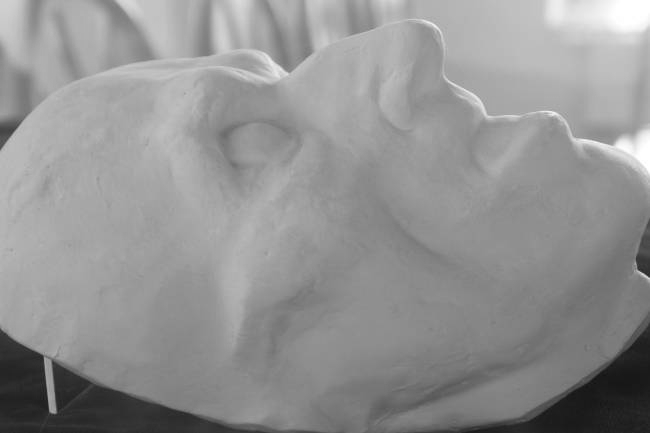
\includegraphics[width=130mm]{./imgs/kaliningrado2.jpg}  
  %\hfill
\end{adjustwidth}
  \caption{Máscara mortuária do filósofo alemão Immanuel Kant (1724-1804)}

\thispagestyle{empty}

\end{figure}
\end{vplace}

\end{absolutelynopagebreak}

%\begin{absolutelynopagebreak}
%\begin{vplace}
%\begin{figure}[H]
%\begin{adjustwidth}{-2.7cm}{}
%  %\centering
%  \vspace{2.7cm}
%  \hspace{0.5cm}
%  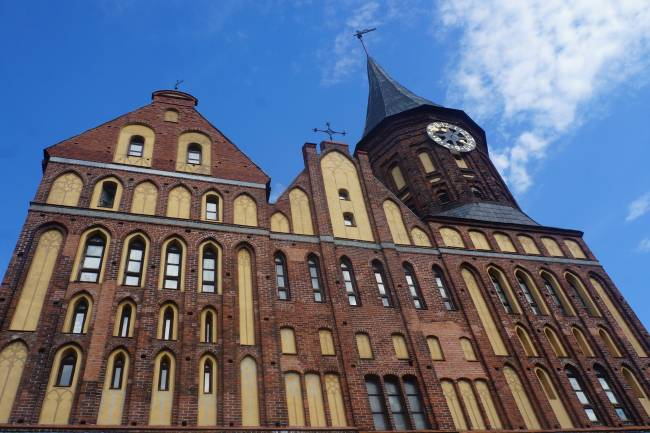
\includegraphics[width=140mm]{./imgs/kaliningrado1.jpg}  
%  %\hfill
%\end{adjustwidth}
%  \caption{Catedral protestante de Königsberg"-Kaliningrado.}%

%\thispagestyle{empty}%

%\end{figure}
%\end{vplace}%

%\end{absolutelynopagebreak}

%\makeatletter\@openrightfalse
%\clearpage{\pagestyle{empty}\cleardoublepage}
\movetooddpage
\addcontentsline{toc}{part}{Kaliningrado (Königsberg) [km 5520]}
\part*{KALININGRADO (KÖNIGSBERG) -- KM 5520\\\medskip\small{{[}A OESTE DE MOSCOU, NÍJNI NOVGOROD, KAZAN,\\SARANSK E SAMARA; A NOROESTE DE VOLGOGRADO\\\vspace{-4pt}(STALINGRADO), ROSTOV-SOBRE-O-DON E SOTCHI{]}}}


\chapter*{Narciso gosta de se mutilar:\\De \emph{Crime e castigo} a crimes sem castigo}
\addcontentsline{toc}{chapter}{[11/07/18] Narciso gosta de se mutilar: De \emph{Crime e castigo} a crimes sem castigo}
%\@openrighttrue\makeatother

\begin{flushright}
\emph{Kaliningrado (Königsberg), 11 de julho de 2018}
\end{flushright}

\section{I. Crimes sem castigo}

Protagonista do romance \emph{Crime e castigo}, do russo Fiódor
Dostoiévski, o ex"-estudante de Direito/jovem intelectual niilista Ródion
Raskólnikov bem apreende que sua época -- tempos de pujança
científico"-industrial, tempos anticriacionistas de Charles Darwin --
está matando Deus, a base transcendental sobre a qual haviam sido
estruturados, histórica e ideologicamente, os princípios éticos da
humanidade. Não à toa, o filósofo alemão Friedrich Nietzsche, leitor
contumaz de Dostoiévski, nos narra, em \emph{A gaia ciência}, a história
de um

\begin{quote}
homem louco que, em plena manhã, acendeu uma lanterna, correu até o
mercado e se pôs a gritar incessantemente: ``Procuro Deus! Procuro
Deus!'' (\ldots{}) Conta"-se também que no mesmo dia o homem louco irrompeu em
várias igrejas e, em cada uma delas, entoou o seu \emph{Requiem aeternam
deo}. Levado para fora e interrogado, limitava"-se a responder: ``O que
são ainda essas igrejas, se não os mausoléus e túmulos de
Deus?''\footnote{Friedrich Nietzsche, \emph{A gaia ciência.} Tradução de
  Paulo César de Souza. São Paulo: Companhia das Letras, 2001, pp.
  147-148.}
\end{quote}

Raskólnikov bem sabia que a suposta loucura da personagem nietzscheana
sintetizava o espírito de sua época. Revogado, então, o Decálogo de
Moisés, o cadáver de Deus só fazia apontar para a obsolescência de um de
seus mandamentos pétreos: \emph{Não matarás.} Afinal, o raciocínio
niilista de Raskólnikov o leva a pensar que, se Deus não existe, tudo é
permitido; assim, apenas a massa ordinária continuará a se aferrar, por
séculos e séculos, amém, a princípios transcendentais putrefatos. Cabe
aos seres extraordinários -- prossegue o niilismo raskolnikoviano --
sepultar de vez o anacronismo judaico"-cristão para fundar uma época em
que o homem (ou, melhor, o super"-homem) se torne o centro e a medida de
todas as coisas.

Quando lemos os livros do Velho Testamento, que característica da
personalidade divina mais salta aos olhos?

\begin{quote}
Urge dar vida por vida, olho por olho, dente por dente, mão por mão, pé
por pé, queimadura por queimadura, ferida por ferida, golpe por golpe.
Eu, o Senhor, teu Deus, sou um Deus zeloso, que castigo a iniquidade dos
pais nos filhos, até a terceira e quarta gerações daqueles que me
odeiam\footnote{\emph{Êxodo}, cap. 21, versículos 23 a 25;
  \emph{Deuteronômio,} cap. 5, versículos 9 a 10.}.
\end{quote}

Ao nos lembrarmos da fúria de Deus que inunda suas criaturas com o
dilúvio e dizima sem mais os habitantes de Sodoma e Gomorra, descobrimos
que a divindade reserva unicamente para si o papel de carrasco. Ocorre
que Kiríllov, personagem dostoievskiana de \emph{Os demônios} e filho
intelectual de Raskólnikov, só faz proclamar: ``Se Deus não existe,
então eu sou Deus. (\ldots{}) Se Deus existe, então toda a vontade é Dele, e
fora da vontade Dele nada posso. Se não existe, então toda a vontade é
minha, e sou obrigado a proclamar o arbítrio''\footnote{Fiódor
  Dostoiévski, \emph{Os demônios.} Tradução de Paulo Bezerra. São Paulo:
  Editora 34, 2004, p. 597.}.

A escatologia de Raskólnikov conclui, portanto, que a coroação do ego só
estará completa quando a espada letal de Deus for desembainhada pela mão
do super"-homem.

Munido, então, de um machado, Raskólnikov vai à casa da usurária Alióna
Ivánovna, para quem o jovem empenhara as últimas quinquilharias de sua
miséria. Chega o momento de a personagem realizar seu experimento
niilista: com duas machadadas certeiras contra a têmpora do ``piolho
usurpador'', Raskólnikov lança mão da terra arrasada moral que o
anarconiilista alemão Max Stirner já defendera em sua obra \emph{O
único e a sua propriedade}:

\begin{quote}
O que é divino é problema de Deus, o que é humano, problema do homem. Eu
não me preocupo com o que é divino, humano, verdadeiro, bom, justo,
livre etc., mas, unicamente, com o que é meu, e não se trata de algo
genérico, mas de algo único, já que eu sou único. Nada significa mais
para mim do que eu mesmo! (\ldots{}) O que eu quiser, eu devo possuir e vou
buscar. O que o homem conseguir amealhar lhe pertence: o mundo me
pertence. O certo é aquilo que me convém\footnote{Max Stirner, \emph{O
  único e a sua propriedade.} Tradução de João Barrento. São Paulo:
  Martins Fontes, 2009, p. 171.}.
\end{quote}

Mas eis que, no momento em que Raskólnikov mata Alióna Ivánovna, a irmã
da velha usurária aparece no apartamento. Ora, é preciso proceder à
queima de arquivo, meu caro, ossos do ofício niilista: o ventre de mais
uma inocente é necessário para o parto do novo mundo. De um momento para
o outro, o utilitarismo de Raskólnikov o transforma de ex"-estudante de
Direito/inquilino inadimplente em duplo homicida. {[}Pequenas empresas,
grandes negócios: quando o microempreendedor Raskólnikov conseguir
arregimentar niilistas suficientes para fundar uma seita política, tomar
o poder e instaurar um regime de terror multinacional, o executivo
soviético Ióssif Stálin lhe ensinará que uma única morte é uma tragédia;
duas, uma decorrência; um milhão, material estatístico.{]}

Ocorre que, antes de desferir as machadadas, Raskólnikov ouviu as
súplicas de suas vítimas, o jovem viu as contorções agônicas em seus
rostos; enquanto aplicava os golpes, a personagem ainda pôde entreouvir
o choro e o ranger de dentes, a suma dor do corpo que estrebucha e
desfalece diante do carrasco. É assim que, após violar a fronteira do
\emph{Não matarás}, Raskólnikov se vê acossado pelo espectro da culpa e
do remorso. {[}Não sabemos, ao certo, se o jovem sofre por causa de suas
vítimas ou se ele padece pelo fato de sua vaidade lhe mostrar que, a
despeito de seus ideais niilistas e grandiloquentes, Raskólnikov não
consegue suportar o fardo de ter aspergido sangue alheio. Assim, o
dostoievskiano em questão não seria, verdadeiramente, um super"-homem
para quem tudo é permitido, mas um cordeiro em pele de lobo, mais um
membro da massa ordinária da qual ele antes tanto queria se apartar.{]}

Diante das agruras morais de Raskólnikov, o niilista romeno Emil Cioran,
em sua obra \emph{Lágrimas e santos}, passa a desancar tanto a
personagem quanto o próprio Dostoiévski:

\begin{quote}
Raskólnikov estava inquestionavelmente certo: de um lado, temos a massa
que vive como um bando de autômatos de acordo com as leis da natureza;
de outro, os eleitos para quem tudo é permitido, uma vez que eles expiam
a vergonha da mediocridade da vida através da intensidade de suas
próprias vidas. Mas por que Raskólnikov falha? Por que ele se vê
consumido pelo remorso depois do crime? Seria possível que Dostoiévski
temesse as consequências de seus próprios princípios? Ora, um homem que
enfrentou a morte já não pensa em quaisquer consequências. A falha de
Raskólnikov nos leva à covardia de Dostoiévski\footnote{Emil Cioran,
  \emph{Tears and Saints} (\emph{Lágrimas e santos})\emph{.} Tradução de
  Ilinca Zarifopol"-Johnston. Chicago: The University of Chicago Press,
  1995, p. 97. Fiz a tradução livre do trecho para o português.}.
\end{quote}

Para Cioran (e Nietzsche), o niilista, muitas vezes, só está à altura de
seu ato no momento do assassínio; pouco depois, a culpa já começa a
consumi"-lo até a medula. Dostoiévski, assim, teria retirado o gênio da
modernidade niilista da lâmpada, mas, assombrado pelos desdobramentos de
suas ideias -- isto é, acossado pela vacuidade ética de sua época --, o
escritor russo teria inoculado em sua personagem os bacilos anacrônicos
do judaico"-cristianismo que só fariam embotar Raskólnikov diante do
vanguardismo de sua heresia. A covardia de Dostoiévski, então, diria
respeito ao medo (e à culpa) de ter dado à luz um sentido de época que
solaparia todas e quaisquer bases para a reciprocidade e a solidariedade
humanas. Ao fim e ao cabo, os répteis só fariam devorar uns aos outros
-- levado às últimas consequências, o darwinismo social de Raskólnikov
não traria tranquilidade nem mesmo aos poderosos, já que, leitores das
lições de \emph{O príncipe}, do florentino Nicolau Maquiavel, eles sabem
que sequer o generalíssimo romano Júlio César está a salvo.

Ocorre que o devir da obra de Dostoiévski se encarrega de dar uma
resposta a Cioran.

Raskólnikov concebe o assassínio e o executa. O protagonista de
\emph{Crime e castigo} formula o plano e suja as mãos de sangue. Tempos
depois, em \emph{Os irmãos Karamázov}, Dostoiévski\footnote{Fiódor
  Dostoiévski, \emph{Os irmãos Karamázov.} Tradução de Paulo Bezerra.
  São Paulo: Editora 34, 2012.} daria vazão àquilo que poderíamos chamar
de divisão letal do trabalho: Ivan, o intelectual niilista, concebe a
morte de seu pai, o bufão Fiódor Karamázov; Smierdiakov, irmão de Ivan e
filho bastardo de Fiódor, executará o parricídio. Membro da
\emph{intelligentsia} revolucionária, Ivan tem muito a perder se sujar
as mãos de sangue; o reles serviçal Smierdiakov, por sua vez, é filho do
estupro de sua mãe pelo pai Karamázov. Ora, a simbologia é inequívoca:
se o Pai diluviano está morto, o pai estuprador não pode permanecer
vivo. Sem ter o que perder a não ser os aguilhões de sua própria
humilhação, Smierdiakov assassina o pai e, numa trama bastante ardilosa,
ainda faz com que a culpa recaia sobre o irmão Dmítri Karamázov, que já
alardeara aos quatro cantos a vontade de matar Fiódor Karamázov, uma vez
que ambos disputavam, encarniçadamente, o amor de Grútchenka, uma das
mulheres mais pungentes da obra de Dostoiévski.

É bem verdade que, ao fim, Ivan Karamázov fica louco, e Smierdiakov se
enforca -- novamente, a simbologia judaico"-cristã em Dostoiévski é
profunda: a razão niilista e utilitária de Ivan se esfacela; assim como
Judas Iscariotes, o traidor de Cristo, Smierdiakov se enforca. O
parricídio, então, acaba revertido contra si mesmo. De qualquer forma, a
escatologia criativa de Dostoiévski, ao acompanhar os sentidos e
ressentimentos de sua época, pôde levar às últimas consequências a
ruptura do \emph{Não matarás}: quando mentor e executor se tornam duas
pessoas distintas, a cisão moral de Raskólnikov -- em russo,
\emph{raskol} significa cisão -- passa a ser administrada de maneira a
minimizar o superaquecimento das máquinas e maximizar a produtividade.

Se lançarmos mão da escatologia criativa de Dostoiévski para aproximá"-la
de nossa própria época, teremos que alterar o título do romance de
\emph{Crime e castigo} para \emph{Crimes sem castigo} em face dos
ataques militares a reboque de \emph{drones. }

Por improvável e exígua que fosse, ainda havia uma possibilidade de
Alióna Ivánovna e sua irmã escaparem das machadadas de Raskólnikov: os
golpes poderiam errar o alvo, as vítimas poderiam se esquivar, o corpo
do carrasco, radicalmente presente, poderia ser ferido de alguma
maneira. É bem verdade que o homicídio concebido e executado pela
personagem já pressupunha um forte princípio de alienação em relação ao
outro -- a alteridade, na verdade, não passava de um meio com vistas ao
alcance de determinado fim. De qualquer forma, a reversão do assassínio
como culpa -- eis o castigo quintessencial em face do crime -- revela um
caráter empático entre algoz e vítimas.

Ora, ninguém escapa de um ataque de \emph{drones.} Ataque matemático,
ataque via satélite, ataque incólume -- não há qualquer possibilidade de
os mandantes ouvirem o choro e o ranger de dentes de suas vítimas --,
ataque sem sobreviventes, ataque, potencialmente, sem ruínas, já que,
com disparos e bombas cirúrgicos, tudo é destruído, tudo é pulverizado.
Tende a zero, inclusive, o horror que, certa vez, o ex"-presidente dos
\versal{EUA} Bill Clinton chamou de \emph{collateral damage} -- as vítimas
inocentes que, não tendo relação com os verdadeiros alvos militares, se
transformam em danos colaterais\footnote{A expressão bombardeada por
  Bill Clinton tem seu sentido desenvolvido no artigo ``Collateral
  Damage: A Brief History of \versal{U.S.} Mistakes at War'' (``Danos colaterais:
  Uma breve história dos erros dos \versal{EUA} nas guerras''), de James
  Griffiths, publicado em 07/10/15 no \emph{site} da \emph{\versal{CNN}}. Eis o
  \emph{link} para o texto: \textless{}\emph{https://cnn.it/2D2srqP}\textgreater{}.}.
Já não há choro e ranger de dentes pelo fato de que quarteirões inteiros
pulverizados por computador sequer apresentam testemunhas. (O pintor
espanhol Pablo Picasso não conseguiria pintar \emph{Guernica} após um
ataque de \emph{drones.})

Em face da divisão letal do trabalho levada a cabo por Ivan Karamázov e
Smierdiakov, Raskólnikov é um aprendiz de feiticeiro; em face de um
ataque de \emph{drones}, Ivan Karamázov e Smierdiakov são contratados,
respectivamente, como engenheiro civil e pedreiro da empreiteira
multinacional que encabeçará as obras de reconstrução da Síria após os
exércitos estadunidense e russo terem devastado o país.

\section{\versal{II}. Narciso gosta de se mutilar}

E se o egoísmo, o utilitarismo e o hedonismo de Raskólnikov, Ivan
Karamázov e Smierdiakov não representassem, inequivocamente, a
maximização das satisfações pessoais? E se, sob a capa de sua volúpia,
Narciso só ficasse escarafunchando suas feridas purulentas como que a
conjuminar prazer e dor?

À primeira vista, a sociedade contemporânea, em sua monomania
competitiva, é formada por sujeitos radicalmente cônscios da necessidade
de exaltar as próprias capacidades para suplantar os demais. Os
currículos que apresentamos em entrevistas de emprego parecem forjados
pelo sarcasmo de Álvaro de Campos:
%, um dos heterônimos de Fernando Pessoa:

\begin{verse}
\small{
Nunca conheci quem tivesse levado porrada.\\
Todos os meus conhecidos têm sido campeões em tudo.\\
(\ldots{})\\[5pt]
Toda a gente que eu conheço e que fala comigo\\
Nunca teve um ato ridículo, nunca sofreu enxovalho,\\
Nunca foi senão príncipe -- todos eles príncipes -- na vida\ldots{}}\footnote{Álvaro
  de Campos/Fernando Pessoa, ``Poema em linha reta''. In: \emph{Fernando
  Pessoa: obra poética.} Rio de Janeiro: Nova Aguilar, 1972, p. 37.}
\end{verse}

A melancolia cabisbaixa e o realismo profundo de Manuel Bandeira, quando
o poeta suspira pela ``vida inteira que podia ter sido 
e que não foi''\footnote{Manuel Bandeira, ``Pneumotórax''. In: \emph{Manuel
  Bandeira: poesia completa e prosa.} Rio de Janeiro: Nova Aguilar,
  2009, p. 81.}, devem ser vedados a todo custo com tarjas pretas.
(Raskólnikov e Ivan Karamázov se tornam executivos da indústria
farmacêutica.) Apresentar o \emph{curriculum vitae} ao lado do
\emph{curriculum mortis} -- isto é, vibrar com as conquistas muitas
vezes frágeis e contingentes sem escamotear as reiteradas derrotas e
frustrações -- equivale a um \emph{harakiri} profissional (e pessoal). É
preciso vestir a camisa, é preciso ser pró"-ativo, é preciso cumprir
todos e cada um dos prazos que se sobrepõem como a imagem tangível da
ansiedade e do desespero, é preciso trabalhar para (muito) além do
horário, é preciso, ainda assim, ter o corpo esbelto (liquidez corpórea,
liquidez laboral), é preciso se exercitar na academia como um
prolongamento doloroso da alienação própria ao escritório. Questionar a
cacofonia da vida inteiramente administrada já não pressupõe uma licença
psiquiátrica -- com a extinção da \versal{CLT} e a degola do \versal{INSS}, Narciso
precisa gostar de se mutilar.

Se entrevíssemos a possibilidade de carreiras estáveis e
bem"-remuneradas, a autoflagelação da formiga ainda poderia se vangloriar
diante da completa insegurança a que a vida tresloucada da cigarra se vê
submetida. Ocorre que, por meio de uma total paródia da famosa fábula do
francês Jean de La Fontaine, o turbocapitalismo radicalmente
contemporâneo já não dá garantias ao sumo esforço da formiga, de modo
que a contingência e a insegurança -- as marcas da vida \emph{hippie} da
cigarra -- também passam a assolar o formigueiro.

Ao invés de permitir a seus funcionários uma carreira prolongada e
bem"-planejada, as empresas transformam o risco e a instabilidade na
segunda natureza do cotidiano profissional. Quando assalariados são
chamados de colaboradores -- à valorização simbólica corresponde a
extinção de direitos trabalhistas --, nem mesmo a ironia cruel de
Machado de Assis ousa engatilhar seu sorriso de canto de boca.
Contratam"-se colaboradores ou sócios -- sujeitos monetários sem
dinheiro, donos de empresas sem capital e meios de produção -- por
projetos: durante um determinado tempo -- 6 meses, 1 ano ou, quando
muito, 2 anos --, o empreendedor pode contar com seu salário. (Ou
não\ldots{}) Depois disso, se a idade útil lhe permitir, será preciso achar
um novo emprego -- ou, melhor, uma nova colocação (termo mais propício
para retratar o caráter móvel e retrátil das pessoas administradas como
coisas.)

Não à toa, a guerra de todos contra todos se acirra: pais perdem a
autoridade sobre os filhos -- a instabilidade econômica esgarça o manto
da tradição --, o falo já não pode titubear, o clitóris intumescido se
torna fálico, casais se divorciam (se é que alguma vez chegaram a se
unir) e amizades se estilhaçam -- afinal, qualquer prenúncio de
intimidade tende a municiar potenciais competidores. Um velho provérbio
árabe se transforma no mantra de Narciso: ``Aquilo que o teu inimigo não
puder saber, não o digas ao amigo''\footnote{Provérbio árabe citado pelo
  filósofo alemão Arthur Schopenhauer na obra \emph{Aforismos para a
  sabedoria na vida.} Tradução de Genésio de Almeida Moura. São Paulo:
  Edições Melhoramentos, 1956, p. 195.}.

Em um contexto de radical solapamento da base de reprodução social da
vida, não nos deve assustar que o conglomerado midiático"-ideológico alce
o nível de exigências narcísicas a patamares estratosféricos (formação
irretocável, corpos esbeltos, pele, dentes e cabelos imaculados), na
mesma medida em que Narciso Raskólnikov Karamázov, para prolongar a
sociopatologia de seu narcisismo, precisa gostar de se mutilar (nesse
caso, indícios de inadequação e depressão não seriam sintomas de
sanidade?). É quando Eros e Tânatos, prazer e dor, sadismo e masoquismo,
utilitarismo e morbidez passam a copular compulsivamente; é quando a
construção utilitária da vida, ao se ver radicalmente deformada pelo
risco e a insegurança, escarafuncha as feridas de Narciso com o punhal
daquilo que poderíamos chamar de inutilidade banal. Ora, à banalidade
utilitária e hedonista dos sujeitos que precisam se mostrar narcísicos,
corresponde a inutilidade banal daqueles que, mais dia, menos dia, serão
substituídos ou proscritos com a mesma celeridade com que se afirmam,
hoje, para além dos demais. A sensação de ser fungível trai o amor de
Narciso por si mesmo: por ter que respeitar a -- ou, pior, por ter que
acreditar na -- autoidolatria, o Narciso insolvente e contingencialmente
empregado passa a se odiar na mesma medida em que precisa se amar, uma
vez que o senso de autodesprezo se insinua pelas muitas frestas daquele
que, a despeito do \emph{outdoor} de si mesmo (o ego como \emph{Você
\versal{S/A}}), já não consegue corresponder à imagem de sua marca.

Se apontássemos a competição dos grandes narcotraficantes mexicanos para
ver quem erige o túmulo mais solene e portentoso, seria possível
redarguir que, em tais carreiras criminosas, a morte é uma eminência
parda de tal vulto que, a bem dizer, é como se Tânatos destronasse Eros
de uma vez e passasse a ditar, com a ampulheta e a foice da morte, todos
e cada um dos parâmetros narcísicos do prazer.

Entretanto, quando observamos o padrão de comportamento dos atiradores
civis, desde o massacre na Columbine High School, no Colorado (\versal{EUA}), em
abril de 1999, passando pelo massacre do Realengo, ocorrido na Escola
Municipal Tasso da Silveira, na cidade do Rio de Janeiro, em abril de
2011, até chegarmos ao mais recente caso na Parkland High School, na
Flórida (\versal{EUA}), no dia 14 de fevereiro de 2018 (apenas para citarmos três
entre as várias tragédias ocorridas), descobriremos que há uma profunda
fusão entre \emph{winners} e \emph{losers}, vida e morte.

Os atiradores escolares tendem a apresentar o perfil dos \emph{nerds}
que, supostamente (e não mais do que supostamente), não se importam em
ser postos em ostracismo. Tidos como párias no esporte e desprezados
pelas garotas, o ímpeto narcísico de tais \emph{losers} se vê
achincalhado a ponto de considerarmos que eles sequer têm amor próprio.
Mas, a partir da adaptação de uma famosa máxima do químico francês
Antoine de Lavoisier, é possível dizer que, na sociedade, nada se perde,
nada se cria, tudo se transforma. Como face reversa (e recíproca) do
narcisismo, o ressentimento do \emph{loser}, via de regra, traz
implicações como a rebeldia no vestuário e no asseio, o isolamento e a
misantropia. Mas, em alguns casos -- casos que, desde o massacre de
Columbine, passaram a compor uma verdadeira dinastia --, o profundo
ressentimento opera como um propulsor que, no limite, pretende
transformar o \emph{loser} em \emph{winner}, o coadjuvante em herói, por
meio de uma vingança viril que, ao mesmo tempo, lance mão do martírio
como derradeira exposição narcísica.

Os atiradores tentam matar todos aqueles e aquelas que os desprezam. Ao
fim e ao cabo, suicidam"-se, mas o martírio, como a tradição
sociopatológica de tais massacres já consagrou, é precedido pela feitura
de vídeos postados no \emph{YouTube}. Agora, eles não poderão ser
simplesmente relegados e/ou esquecidos. Sempre que os sobreviventes e
parentes se lembrarem das vítimas, o narcisismo dos \emph{losers} será
vivenciado e veiculado, ainda que eles não possam aferir, de forma
utilitária e hedonista, os louros de sua vitória de Pirro após a morte.
Nesse caso, à morte em vida dos \emph{losers} em termos do hedonismo
narcísico, corresponde a vida após a morte (sem Deus e sem a eternidade)
dos \emph{winners} que, em meio à dinastia letal a que dão continuidade,
os eleva à condição de mártires. É quando Eros e Tânatos, prazer e dor,
sadismo e masoquismo, utilitarismo e morbidez passam a copular
compulsivamente; é quando a destruição utilitária da vida escarafuncha
as feridas de Narciso com os revólveres e pistolas da inutilidade banal.

Arrematemos este ensaio com o relato do suicídio midiático do jovem
chinês Wu Yongning, 26 anos, famoso escalador de edifícios com
centenas de milhares de seguidores nas redes sociais.

No dia 07 de novembro de 2017, Wu subiu ao cume de um arranha"-céu de 62
andares (190 metros de altura) na cidade de Changsha, no sudeste da
China. O jovem posicionara seu celular, estrategicamente, para poder
gravar todas e cada uma de suas acrobacias junto ao parapeito do
edifício.

Com uma mistura de ansiedade e náusea -- aparições somáticas de Eros e
Tânatos --, assistimos ao vídeo de dois minutos e nove segundos, ao
longo do qual o jovem se debruça sobre o parapeito do prédio, desce a
perna direita, desce a perna esquerda, se escora junto ao parapeito com
os antebraços e, pênsil como o pólen, começa a fazer barra vertical --
uma, duas, três vezes -- como se estivesse circundado pela areia da
praia de Copacabana. Súbito, a situação se complica, Wu perde o
equilíbrio -- o jovem tenta, sem sucesso, levar o dorso até o parapeito,
mas lhe faltam forças. Com a palma das mãos suadas e a respiração
ofegante, os espectadores ainda ouvimos o grito agônico e esganiçado de
Wu antes de o jovem despencar para o estrelato da morte.

``Querido Wu, essa foi a sua melhor \emph{performance. Show must go on:}
nós nunca esqueceremos você!'' -- diz o comentário repleto de curtidas
de uma seguidora de Wu, cuja morte vivificada sentencia que Narciso, de
fato, adora se mutilar\footnote{Eis o link para o vídeo do suicídio
  midiático de Wu Yongning postado no \emph{YouTube}: \textless{}\emph{https://bit.ly/2G6mITU}\textgreater{}. Este texto foi publicado em 13/04/18 no blog ``Estado da Arte'', do
  jornal \emph{O Estado de S. Paulo}.}.

\chapter*{O 11º mandamento do evangelho\\segundo Immanuel Kant}
\addcontentsline{toc}{chapter}{[12/07/18] O 11º mandamento do evangelho segundo I. Kant}

\begin{flushright}
\emph{Kaliningrado (Königsberg), 12 de julho de 2018}
\end{flushright}

Por não fazer parte do território contíguo da Federação Russa, a cidade
de Kaliningrado, à beira do Mar Báltico, entre a Polônia e a Lituânia, é
o que a Geografia chama de exclave.

Entre os séculos \versal{XV} e \versal{XVII}, a antiga cidade de Königsberg, fundada por
cavaleiros teutônicos, pertenceu à Polônia.

Com a unificação e o fortalecimento militar da Alemanha, no fim do
século \versal{XIX}, Königsberg passou a fazer parte do \emph{Reich}.

Ao caminhar pelo centro da cidade, deparo com prédios de arquitetura
alemã transpassados por letreiros em cirílico. É assim que, com uma
fachada entalhada em madeira rústica, o {\MinionPro{Баварский Pесторан}}
(\emph{Bavarski Restoran}, Restaurante Bávaro) anuncia suas iguarias que
remontam à época da dominação germânica; um prédio acinzentado e austero
de quatro andares, hoje sede de um instituto tecnológico próximo da
praça central de Kaliningrado, já abrigou as instalações da temível
\emph{Geheime~Staatspolizei} (Polícia Secreta do Estado), que os
nazistas chamavam pelo acrônimo de Gestapo.

Com a vitória dos Aliados na Segunda Guerra Mundial, o primeiro"-ministro
inglês Clement Attlee, o presidente dos \versal{EUA} Harry Truman e o ditador
soviético Ióssif Stálin se reuniram em Potsdam, cidade situada na região
leste da Alemanha, entre 17 de julho e 02 de agosto de 1945, para
redesenhar o mapa da Europa segundo suas pretensões geopolíticas.

Acordou"-se que a cidade de Königsberg, com localização sumamente
estratégica à beira do Mar Báltico, passaria a fazer parte da União
Soviética.

Com o falecimento do bolchevique Mikhail Kalinin, que participara da
Revolução Russa de 1917, Königsberg foi rebatizada como Kaliningrado.

Entre 1946 e 49, a população alemã foi expulsa da cidade, ocorrendo,
então, sua ocupação (a tomada do butim) por cidadãos soviéticos.

Königsberg/Kaliningrado é famosa por ser a cidade onde nasceu, viveu e
morreu o filósofo alemão Immanuel Kant.

Com sua rígida disciplina prussiana, Kant costumava caminhar pela cidade
diariamente e sempre no mesmo horário. Os conterrâneos do filósofo
chegavam até mesmo a acertar seus relógios com as caminhadas kantianas.

Consta, ademais, que Kant ligava a cabeceira de sua cama à maçaneta da
porta do banheiro com um fio de barbante, para que, quando fosse fazer
suas necessidades fisiológicas de madrugada, o filósofo fosse
devidamente guiado e não perdesse seu precioso tempo de descanso; assim,
suas reflexões e escritos poderiam ser maximizados durante o dia.

Certo fim de tarde, porém, fez o impossível acontecer: Kant se atrasou
em sua caminhada diária. (Sumamente atordoado, até mesmo o fio de
barbante se rompeu.)

Os pacatos moradores de Königsberg ficaram em polvorosa: mas o que teria
acontecido ao nosso filósofo?

Teria Kant sofrido um acidente?

Meu Deus, teria Kant falecido?!

{[}O puritanismo protestante tentava sufocar a mais ínfima (e
pecaminosa) especulação de que o digníssimo Immanuel Kant pudesse ter se
demorado em alguma casa de tolerância nas regiões obscuras de
Königsberg.{]}

Ora, meu Deus, mas o que foi que aconteceu?!

Algo muito, mas muito sério sucedera, pois nada nesse mundo poderia
fazer com que Kant se atrasasse em sua caminhada diária.

Alarmados, os moradores acorreram à casa do filósofo.

Lá chegando, os conterrâneos encontraram Kant todo desalinhado e sem sua
peruca grisalha característica, o que logo os fez pensar que o filósofo
fora acometido por algum grave problema de saúde.

Não fora isso, no entanto, que conseguira abalar a férrea disciplina
prussiana de Kant.

Aos 65 anos, 2 meses e 22 dias, o autor da \emph{Crítica da razão pura}
e da \emph{Crítica da razão prática} se atrasara, pela primeira vez na
vida, ao ficar sabendo que, com a tomada de assalto da Bastilha, a
prisão política de que o absolutismo monárquico lançava mão, a Revolução
Francesa irrompera em Paris. Königsberg e o mundo jamais esqueceriam o
dia 14 de julho de 1789.

Immanuel Kant tornara sumamente famosa a utopia do imperativo categórico
ético, segundo a qual todos e cada um de nós, ao agirmos, devemos nos
balizar por parâmetros passíveis de universalização, de tal maneira que
os demais só venham a ser positivamente afetados por nossas ações. Ao
agir, então, eu sempre devo me colocar no lugar do outro e respeitá"-lo
não como um meio (um instrumento) para os meus fins egoístas, mas como
um fim em si mesmo, isto é, como um sujeito ontológica e igualmente
detentor de dignidade.

Se eu dissemino a mentira e a extorsão, a violência e a pilhagem, estou
autorizando todos e cada um dos meus semelhantes a agir conforme os
mesmos parâmetros. Logo, a guerra de todos contra todos se estabelece.

Se, no entanto, eu agir segundo os princípios da retidão e da
reciprocidade, todos os demais, intrinsecamente respeitados, também
poderão fazê"-lo, de tal maneira que, em meio à utopia kantiana do
imperativo categórico ético, seria possível alcançar a paz perpétua.

{[}Pouco passível de dobrar a primeira esquina da história humana
repleta de choro e ranger de dentes, a suma cordialidade do imperativo
categórico ético bem pode ser imaginada em meio à gentil (e provinciana)
Königsberg de Kant, cidadezinha em que todos os habitantes se conheciam
e jamais deixavam de dar bom dia, boa tarde e boa noite entre as
carruagens e igrejas, tavernas e casas de tolerância.{]}

Quando irrompe a Revolução Francesa, a promessa de disseminação de
governos republicanos que acabassem com as arbitrariedades do
absolutismo monárquico faz com que Kant projete que, enfim, o imperativo
categórico ético ultrapassaria os limites de Königsberg e passaria a
balizar as relações entre os cidadãos, as cidades e os Estados do mundo segundo parâmetros racionalmente constitucionais.

Eis, segundo Kant, a resposta para a questão sobre o que seria a
essência do Iluminismo.

A utopia do imperativo categórico ético é tão revolucionária que ela
ultrapassa o republicanismo iluminista de Kant, saúda o clamor por
liberdade, igualdade e fraternidade dos revolucionários franceses,
aplaude o ardor socialista por uma terra sem amos e, ao fim e ao cabo,
desemboca no mais radical, coerente e responsável anarquismo. Senão,
vejamos.

Kant, obviamente, não era ingênuo a ponto de pressupor que o imperativo
categórico ético ocorreria no éter, isto é, em condições puramente
arquetípicas, abstratas e em meio à profunda desigualdade jurídica,
econômica e social de sua época. A utopia kantiana de indivíduos
reciprocamente cordatos pressupõe a universalização -- em termos
propriamente iluministas, a racionalização -- de tal atmosfera para o
todo social.

Se a sociedade fosse organizada segundo os parâmetros do imperativo
categórico ético, com leis que norteassem a reciprocidade entre
Estados, cidades e cidadãos, o todo e as partes (os indivíduos) se
correlacionariam de forma coerente e orgânica. No limite, os indivíduos
poderiam fazer equivaler a universalidade utópica da lei regida pelo
imperativo categórico com suas próprias consciências, de tal maneira que
cada sujeito racional se transformasse em uma carta constitucional em
miniatura. Nenhuma autoridade precisaria me dizer, então, o que fazer
para respeitar o outro como alguém igual a mim mesmo -- a bem dizer,
como parte de mim mesmo, já que o outro convive comigo em sociedade.

O sujeito autônomo e consciente de si e do outro, para além do jugo da
lei que já lhe seria exterior, projeta, assim, o limite da utopia
kantiana que desembocaria no mais rematado e revolucionário anarquismo.

Se quisermos traçar uma genealogia para o imperativo categórico ético de
Kant, poderemos considerá"-lo uma secularização filosófica da regra de
ouro, princípio basilar para as mais diversas tradições religiosas.
Nesse sentido, eis o que nos revela o seguinte fragmento da obra \emph{A
grande transformação}, de autoria da estudiosa de religiões Karen
Armstrong:

\begin{quote}
Não faças aos outros o que não farias a ti mesmo. (\ldots{}) Se, por exemplo,
toda vez que nos sentíssemos tentados a tecer um comentário hostil sobre
um colega, um irmão ou um país inimigo, pensássemos em como nos
sentiríamos se o mesmo comentário se referisse a nós -- e desistíssemos
de tecê"-lo --, superaríamos a nós mesmos. Esse seria um momento de
transcendência. Se tal atitude se tornasse habitual, poderíamos viver
num \emph{ekstasis} permanente, não porque entramos num transe exótico,
mas porque ultrapassamos as fronteiras do egocentrismo. (\ldots{}) O teste é
simples: se nossas convicções -- seculares ou religiosas -- nos tornam
hostis, intolerantes e maldosos em relação à fé alheia, não são
``profícuas''. Se, porém, nos impelem a agir compassivamente e a honrar
o estranho, são boas, úteis e válidas. Esse é o teste da verdadeira
religiosidade em todas as grandes tradições\footnote{Karen Armstrong,
  \emph{A grande transformação}. Tradução de Hildegard Feist. São Paulo:
  Companhia das Letras, 2008, p. 14; pp. 413-414.}.
\end{quote}

Ao nos lembrarmos da história do século \versal{XX} e do monte de ruínas a que a
Königsberg de Kant foi reduzida pelos bombardeios da Segunda Guerra
Mundial, bem constatamos o adiamento (quiçá, a suma impossibilidade) da
bandeira utópica hasteada pelo imperativo categórico ético de Kant.

Ocorre que, a despeito da cordialidade tão protestante quanto
provinciana de Königsberg -- cidade da qual Kant jamais teria saído em
seus longevos 80 anos de vida --, o filósofo conseguiu entrever alguns
pontos cegos para sua utopia ética -- situações aporéticas em que não
seria possível exercer o imperativo categórico de forma alguma;
situações radicalmente amorais que parecem ter escapado até mesmo à
onisciência de Deus.

Imaginemos, por exemplo, a situação de dois náufragos que tentam
sobreviver, desesperadamente, apoiados em uma tábua de madeira.

\pagebreak

Logo se torna patente para os dois pobres diabos que a flutuação da
tábua em meio às águas não comportará dois sobreviventes -- suponhamos
que se trate de um naufrágio ocorrido no Mar Báltico, perto da orla de
Königsberg, de modo que os gritos e clamores por socorro pudessem
acossar as madrugadas regradíssimas de Kant com a agonia do pesadelo.

Se Fritz só puder sobreviver ao naufrágio alijando Eugen da tábua de
salvação (e vice"-versa), não será possível exercer o imperativo
categórico ético, uma vez que Fritz deve aniquilar Eugen para continuar
vivo -- neste caso, o outro tem que ser transformado em um instrumento
radical da minha vontade, que, por sua vez, se vê reduzida à mais
bestial luta pela sobrevivência.

Diante do buraco negro da razão prática convertida na mais impura
desrazão, Kant se vê compelido a denegar as seguintes palavras de Jesus
Cristo:

\begin{quote}
Ouvistes o que foi dito: olho por olho e dente por dente. Eu, porém, vos
digo que não resistais ao mal; mas, se alguém te bater na face direita,
oferece"-lhe também a outra; e àquele que quiser pleitear contigo e
tirar"-te a túnica, oferece"-lhe também a capa\footnote{\emph{Evangelho segundo
  Mateus}, capítulo 5, versículos 38 a 40.}.
\end{quote}

(O desespero protestante de Kant luta para abjurar a vontade blasfema de
responsabilizar Deus por tamanho desatino em Sua criação.)

Imaginemos, no entanto, que, da planície de Kaliningrado, irrompa,
subitamente, uma enorme montanha. (Afinal, Königsberg, do alemão, quer
dizer Montanha do rei.)

Imaginemos, ademais, que os alpinistas Immanuel, Fritz e Eugen estejam
quase alcançando o cume da montanha mágica atados por uma mesma corda
que os transpassa pela cintura.

Súbito, Eugen se desequilibra e não consegue mais se agarrar à montanha.

Eugen só não despenca imediatamente porque a corda o ata a Fritz.

Não suportando o peso de Eugen, Fritz também acaba se desgarrando da
montanha.

Fritz só não despenca imediatamente porque a corda o ata a Immanuel.

Agora, o pobre Immanuel luta, de forma inglória, para se manter agarrado
à montanha tendo que suportar o enorme peso de Fritz e Eugen.

Para Immanuel, agir segundo os parâmetros de Cristo significa ser
totalmente solidário à morte de Fritz e Eugen. Em outras palavras, para
proceder à imitação de Cristo, Immanuel precisa ser crucificado.

Logo ocorre a Immanuel, no entanto, uma ideia mais humana do que
kantiana -- uma saída racional mais prática do que pura: o alpinista que
ainda depende das próprias forças saca uma faca do bolso da calça e, com
sumo pesar (e alívio) no coração, corta a corda que o ata a Fritz.

Para salvar a própria pele, Immanuel precisa fazer com que a lei da
gravidade mate Fritz e Eugen.

Ora, o que é preferível: um mártir ou um sobrevivente?

A despeito de rezar para Jesus Cristo há mais de 2 mil anos, a
humanidade não parece ter dúvidas.

Tanto é assim que, para tal situação de aporia das razões pura e prática
-- situação blasfema que parece transformar a onisciência de Deus em
cumplicidade --, o Código Penal não impõe sanções para Immanuel.

Ao condenar Fritz e Eugen à lei da gravidade para salvar a própria pele,
Immanuel sai incólume diante da lei penal, que, nesse caso, o considera
inimputável.

Para a nossa sociedade, salvar a própria pele à custa do martírio só é
digno de ser ovacionado quando o exemplo puder ser devida e
hermeticamente isolado em cruzes e pedestais. No mais, salve"-se quem
puder.

Ora, o que é preferível: um mártir ou um sobrevivente?

Em meio às ruínas fumegantes da Königsberg bombardeada por ingleses,
norte"-americanos e soviéticos, o soldado alemão/sobrevivente Fritz Eugen
Kant sentencia:

-- Na guerra, eu não posso rezar segundo o princípio do \emph{Não
matarás}. Na guerra, das tábuas da lei que se confundem com os
escombros, resta apenas o 11º mandamento: espero não matar.

\clearpage{\pagestyle{empty}\cleardoublepage}
\movetooddpage
\addcontentsline{toc}{part}{A bordo do voo que vai de Kaliningrado (Königsberg) a São Petersburgo}
\part*{A BORDO DO VOO QUE VAI DE\\KALININGRADO (KÖNIGSBERG)\\A SÃO PETERSBURGO}

\chapter*{Nostalgia do absoluto}
\addcontentsline{toc}{chapter}{[13/07/18] Nostalgia do absoluto}

\begin{flushright}
\emph{Entre Kaliningrado (Königsberg) e\\ São Petersburgo, 13 de julho de 2018}
%\emph{A bordo do voo que vai de Kaliningrado (Königsberg)\\a São Petersburgo, 13 de julho de 2018}
\end{flushright}

À diferença da policromia vibrante que marca as igrejas ortodoxas, a
catedral protestante de Königsberg desponta com austeros tijolinhos
marrons entremeados por janelas e arcos amarelos e contritos, como se a
arquitetura da igreja quisesse expiar os pecados dos fiéis.

Se a aura da catedral não me impressiona, o museu que fica na cúpula da
igreja me deixa atônito ao expor a máscara mortuária do filósofo alemão
Immanuel Kant.

O último semblante de Kant é sumamente macilento; não há traço de carne
ou gordura, como se a evasão da alma também tivesse surrupiado o corpo
do filósofo. Ossos bem pronunciados circundam seus olhos grandes e
fundos como charcos; no meio do nariz fino, pontudo e de narinas
oblongas, uma protuberância óssea sobe e desce como a corcova de um
camelo; bochechas aradas por vincos profundos; o detalhe que me chama
mais a atenção, porém, está na boca de Kant: a despeito dos lábios
inexpressivos, a boca parece entreaberta, como se Kant ainda quisesse
dizer algo. Todo o restante de seu rosto está apaziguado com o término
da vida, à exceção de sua boca loquaz.

O que a máscara mortuária de Immanuel Kant me diria se pudesse falar?

Desço até a igreja propriamente dita para assistir a um concerto de
órgão.

O último concerto que eu havia visto, em julho de 2015, me pegou de
surpresa: ao entrar na pequena igreja da Universidade de Loyola, à beira
do lago Michigan, em Chicago, um órgão denso e efusivo me fez sentir, em
cada fímbria do corpo, a visceralidade de um aforismo do filósofo romeno
Emil Cioran, para quem os acordes de um órgão são degraus celestiais que
aproximam o ser humano do absoluto. Toda a fragilidade que nos constitui
parece reconciliada: o órgão ressoa a presença imediata e tangível de
Deus.

O órgão altivo e barroco redime a austeridade da catedral de Königsberg.

Uma legião de anjos infantis e alados se posta junto às múltiplas partes
do órgão, que, como sói acontecer, fica sobrelevado em relação aos
fiéis. Quando o órgão começa a ressoar, os anjos tocam as trompas e
trompetes como o prenúncio da aterrissagem divina.

Há toda uma mística liberada pela sucessão infinda de acordes graves e
agudos, como se o órgão, qual um tapete voador, nos fizesse descer até o
vale da mais densa prospecção existencial para, em seguida, nos alçar ao
cume sublime da cura.

Como que oriundas dos arabescos dourados que encimam os tubos delgados e
prateados do órgão, mil mãos compassivas nos elevam e enlevam: não há
solidão possível, a música transborda o sentido, o órgão religa a ponte
(o cordão umbilical) com o absoluto pela sucessão de nuvens de seus
acordes.

\pagebreak

O filósofo alemão Arthur Schopenhauer sentenciou certa vez\footnote{Arthur
  Schopenhauer, \emph{O mundo como vontade e representação.} Tradução de
  M. F. Sá Correia. Rio de Janeiro: Contraponto, 2001.} que o movimento
essencial da música, com sua forma pura, indômita e desprovida da dor
semântica das palavras, consegue expressar, com o máximo de
visceralidade e mimese, o ardor da vontade humana, suas idas e vindas,
suas contradições que explodem em paradoxos e fúria; a pura forma
musical, para Schopenhauer, contém, acompanha e liberta a nervura da
paixão em seu ardor, a nervura da melancolia em seu suspiro, a nervura
do sonho em sua espera, a nervura da tristeza em seu pranto, a nervura
do amor em seu acalento, a nervura da alegria em seu canto, a nervura da
saudade em sua nostalgia.

Eu não tenho dúvida de que o ateu Arthur Schopenhauer sentiu essa
descoberta em cada fímbria de seu corpo enquanto ouvia um concerto de
órgão em uma igreja que ele e seu discípulo revolto Friedrich Nietzsche,
musicófilo contumaz como Schopenhauer, chamavam de sepulcro de
Deus\footnote{Friedrich Nietzsche, \emph{A gaia ciência.} Tradução de
  Paulo César de Souza. São Paulo: Companhia das Letras, 2001, pp.
  147-148.}.

O órgão é a própria nostalgia do absoluto.

Quando ressoa suavemente, o órgão é a mãe que entoa uma cantiga de ninar
para o filho.

O órgão sobrelevado em relação aos fiéis lembra a aparição de Deus a
Moisés no cume do Sinai.

Súbito, me ocorre a razão pela qual os sobreviventes ao cerco que os
nazistas impuseram a São Petersburgo quiseram fazer, em plena avenida
Niévski, sob a tempestade de aço e as labaredas das ogivas, uma
apresentação da \emph{Sinfonia n.º 7}, que Dmítri Chostakovitch
compusera em homenagem à cidade sitiada.

Entre 08 de setembro de 1941 e 27 de janeiro de 1944 -- longos,
famélicos, friíssimos e infectos 872 dias --, São Petersburgo (então
rebatizada como Leningrado) se viu cercada pelas tropas hitleristas.

Inanição.

Canibalismo.

Frio -- o frio que exaure, com o tremor dos corpos reduzidos a sacos de
ossos, a última energia da sobrevivência, o frio cujas rajadas de vento
queimam e cortam a pele fina como papel vegetal com a avidez de chicotes
e punhais.

Já não há como esconder a morte a sete palmos do chão -- não há tempo e
força para cavar sepulcros, é preciso aproveitar as crateras abertas
pelas bombas como cemitérios a céu aberto.

Crateras como covas, crateras como trincheiras.

Cadáveres e soldados.

Cemitério dos vivos.

Ainda assim, a resistência de Leningrado decide, contra toda a
racionalidade utilitária, apresentar a \emph{Sinfonia n.º 7} em plena
avenida Niévski.

Todos estão cientes de que podem morrer como moscas em meio ao
bombardeio alemão.

Todos estão cientes de que caminhar (ou, melhor, claudicar) até a
Niévski envolve o risco de morrer de frio e exaustão.

Ora, quem tem medo da morte na Leningrado sitiada?

No inferno, a morte redime.

Queremos ouvir Chostakovitch, queremos vibrar em dó maior -- se, com a
sinfonia atonal das ogivas, esse for o nosso réquiem, morreremos
reconciliados.

Que é a fome diante da sobrevivência?

Não só de pão vive o homem.

Que é o frio diante da sobrevivência?

Entre os escombros, a esperança trêmula como nossos ossos nos
acalentará.

Que é a exaustão diante da sobrevivência?

A falta de fé é o que nos vai exaurir.

Imaginemos que, no Natal de 1941 (1942 e 1943), os sobreviventes ao
cerco de Leningrado, quais esqueletos ambulantes, se abraçaram ao redor
de um maestro maltrapilho, cuja batuta era um semipedaço de arame, de
uma orquestra de zumbis que mal conseguiam soerguer seus instrumentos e
de um piano alquebrado, cuja cauda fora amputada por uma granada.

Tal concerto surrealista só aconteceu porque, como bem sabia o
compatriota dos sobreviventes de Leningrado Fiódor Dostoiévski, os seres
humanos não apenas vivem -- nós buscamos uma razão para viver, nós
buscamos uma razão para continuar a viver, nós buscamos uma razão para
continuar a continuar.

Tal concerto surrealista, réquiem à vida e ode à morte, encarna a
nostalgia do absoluto na Leningrado sitiada em que a mera menção à
justiça de Deus mais parecia um acinte -- o mais viscoso escárnio.

No dia 25 de dezembro de 1943, algum poeta teve a ideia de transportar
um órgão para o coração da avenida Niévski: as flautas da \emph{Sinfonia
n.º 7} dariam lugar aos trovões dos acordes que já se faziam mais
altissonantes do que as explosões -- pouco mais de um mês depois, o
cerco a Leningrado seria levantado pelo Exército Vermelho.

Consta que, quando os soldados russos chegaram à avenida Niévski, eles
não acreditaram nos próprios olhos no momento em que viram uma roda de
cadáveres de mãos dadas ao redor de um maestro que morrera em pé,
congelado, enquanto regia o penúltimo acorde de Chostakovitch.

%\pagebreak
%\clearpage
%\thispagestyle{empty}

\movetoevenpage
\begin{absolutelynopagebreak}
\begin{vplace}
\begin{figure}[H]
\begin{adjustwidth}{-2.7cm}{}
  %\centering
  \vspace{-1.8cm}
  \hspace{2.2cm}
  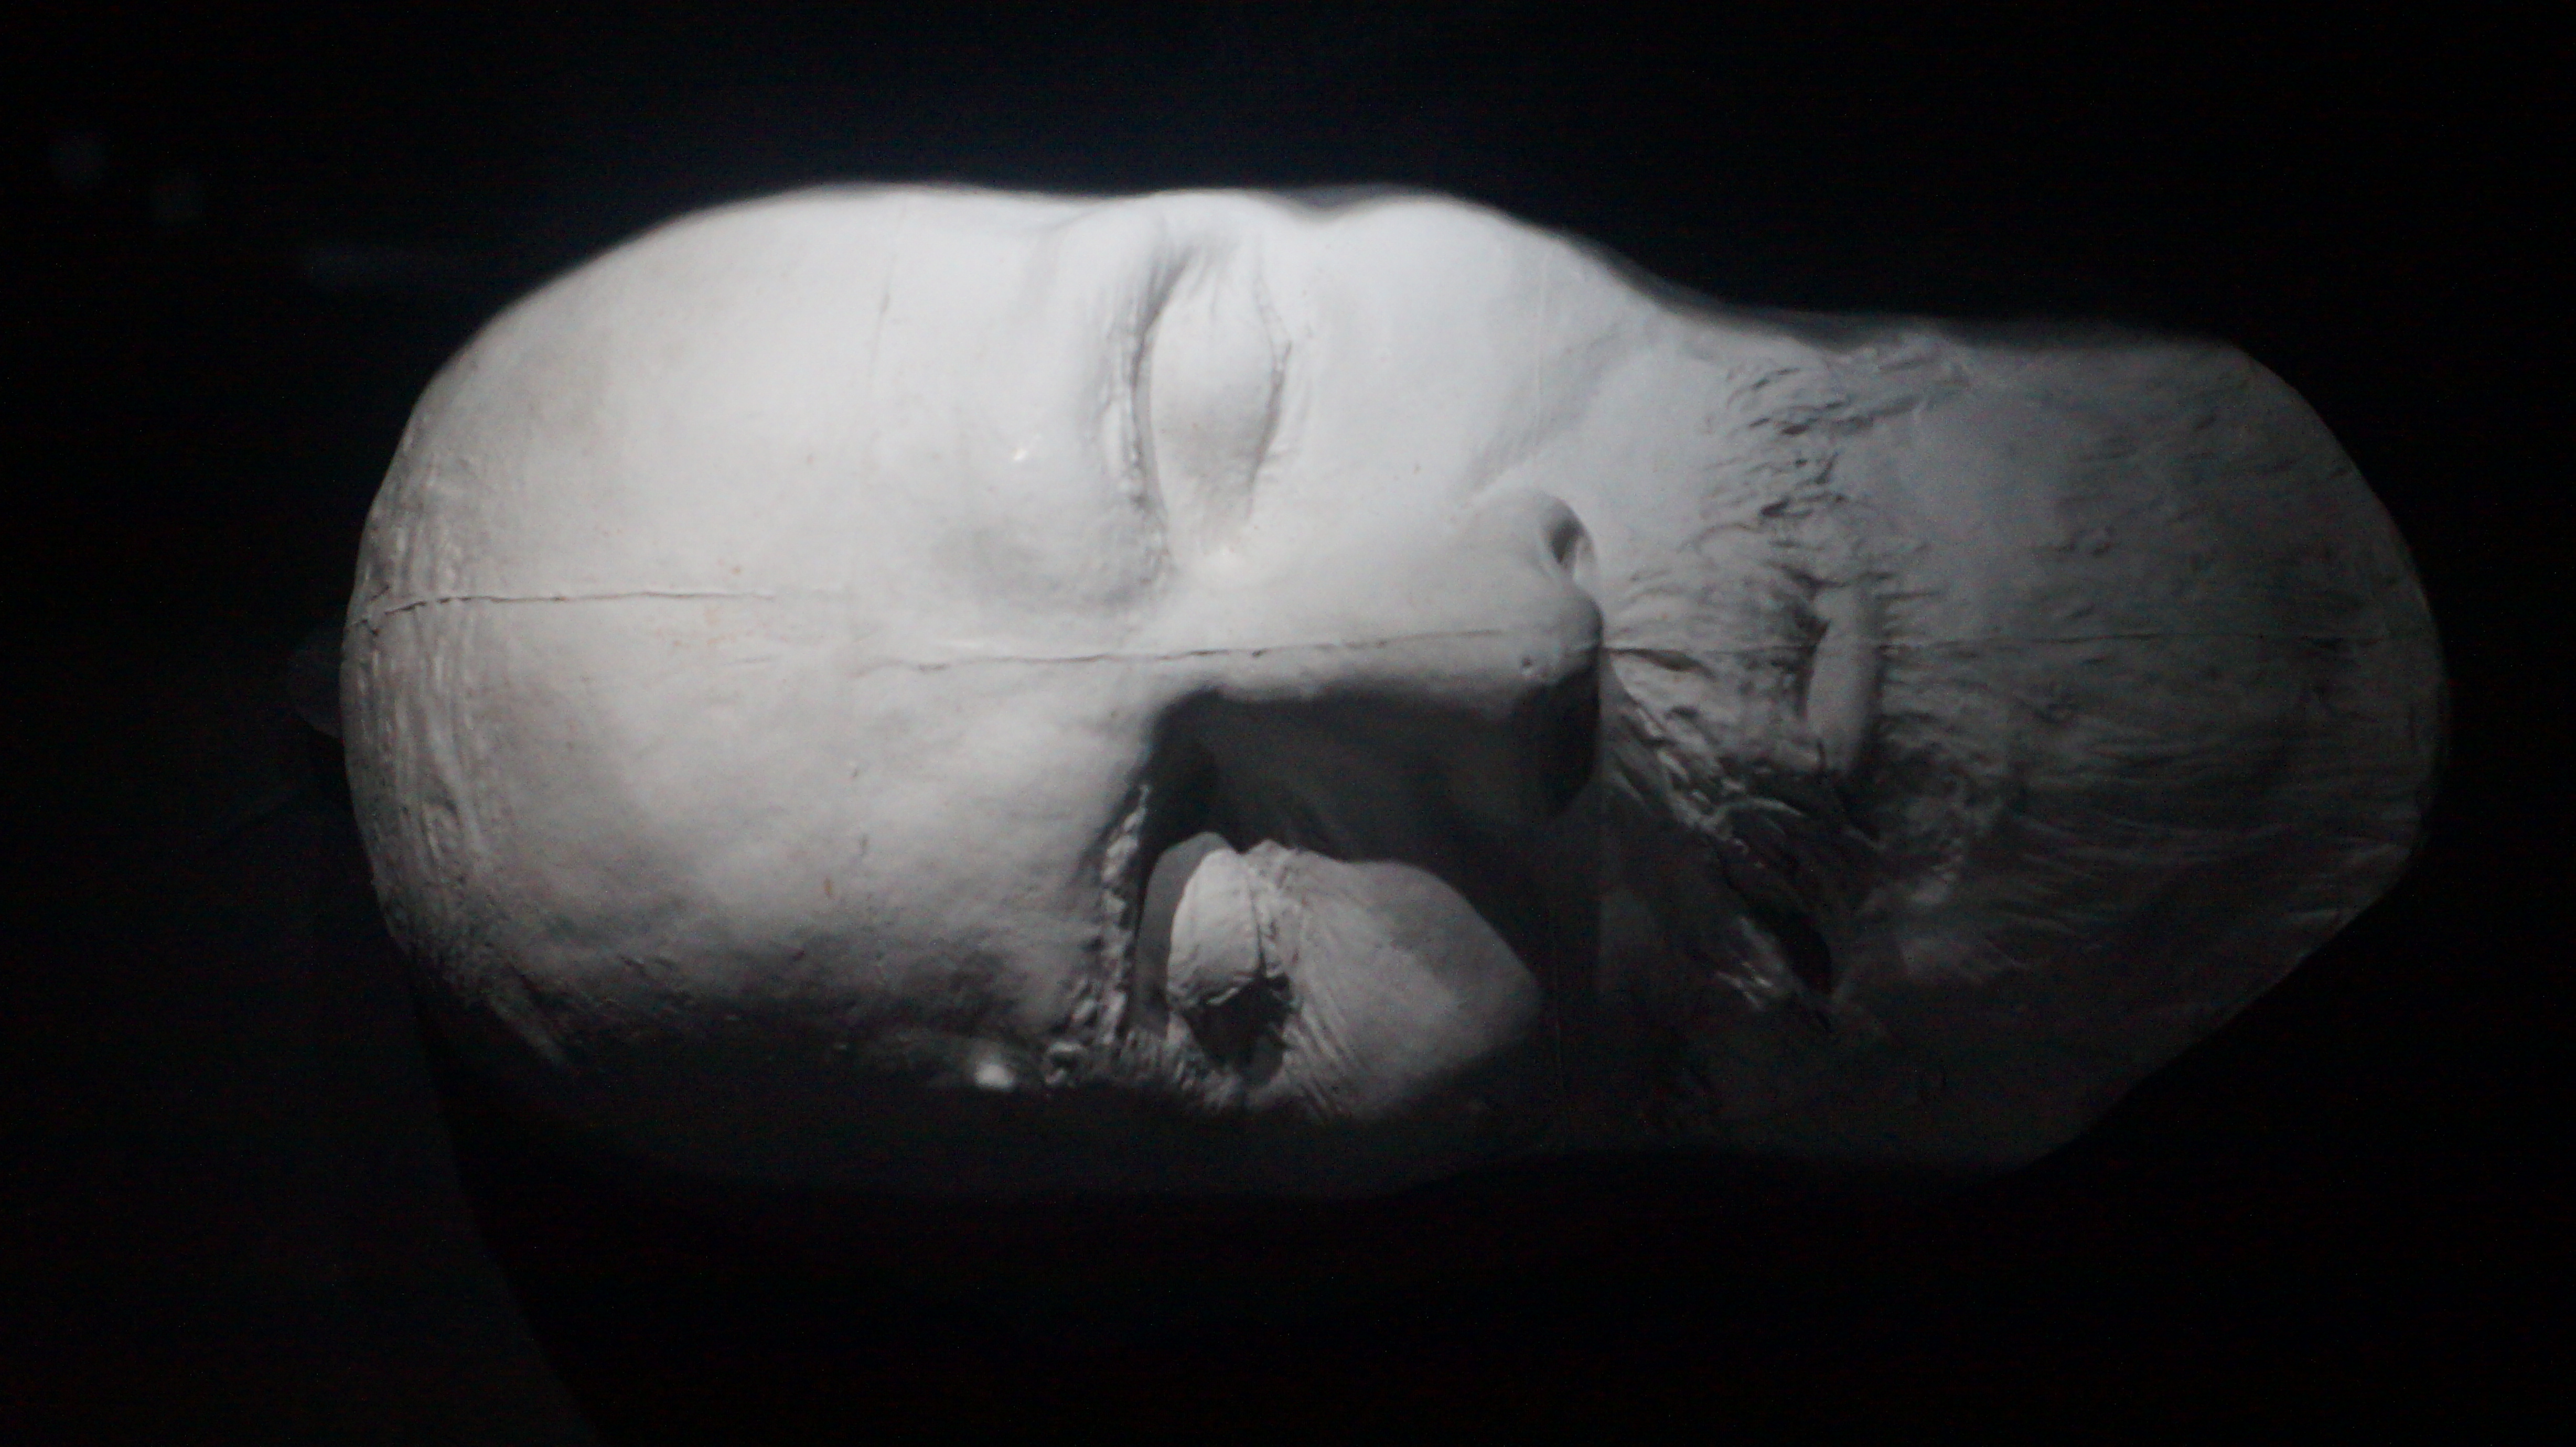
\includegraphics[angle=270,width=100mm]{./imgs/petersburgo2.jpg}  
  %\hfill
\end{adjustwidth}
  \caption{Máscara mortuária do escritor russo Fiódor Dostoiévski (1821-1881)}

\thispagestyle{empty}

\end{figure}
\end{vplace}

\end{absolutelynopagebreak}

%\makeatletter\@openrightfalse
%\clearpage{\pagestyle{empty}\cleardoublepage}
\movetooddpage
\addcontentsline{toc}{part}{São Petersburgo [km 6465]}
\part*{SÃO PETERSBURGO -- KM 6465\\\medskip\small{{[}A NOROESTE DE MOSCOU, NÍJNI NOVGOROD, KAZAN, SARANSK,\\SAMARA, VOLGOGRADO (STALINGRADO), ROSTOV-SOBRE-O-DON\\\vspace{-4pt}E SOTCHI; A NORDESTE DE KALININGRADO (KÖNIGSBERG){]}}}


\chapter*{Entre a cruz e a espada:\\A Rússia sob o punho de Vladímir Putin}
\addcontentsline{toc}{chapter}{[14/07/18] Entre a cruz e a espada: A Rússia sob o punho de Vladímir Putin}
%\@openrighttrue\makeatother

\begin{flushright}
\emph{São Petersburgo, 14 de julho de 2018}
\end{flushright}

Vladímir Vladímirovitch Putin nasceu em Leningrado, antigo nome de São
Petersburgo até o colapso da União Soviética, que ocorreu em dezembro de
1991.

Em um bar da rua Rubinstein, uma das travessas da avenida Niévski, no
coração da cidade, entro em contato com o sexagenário Vassili
Vassílievitch Kuznetsov, que, a despeito de ser um putinista ferrenho,
me pede que seu nome verdadeiro não seja divulgado. ``Sabe como é, né? A
Rússia e o livre pensamento não têm lá muitas afinidades eletivas'',
sentencia Kuznetsov.

A seguir, compartilho com vocês os principais trechos de nosso diálogo
entremeado por um sem"-número de doses de cerveja e vodca.

\textsc{eu:} Quer dizer então que o senhor fala amém para o fato de
Vladímir Putin ter blindado seu antecessor e padrinho político Boris
Iéltsin de quaisquer investigações judiciais por parte da Procuradoria
Federal?

\textsc{vassili vassílievitch kuznetsov:} Antes de mais nada, jovem, não
precisa me chamar de ``senhor''. O Senhor sequer existe no céu solitário
e silencioso, então deixemos de cerimônias. Em seguida, é preciso dizer
que as suas colocações simplesmente desconsideram a história
encarniçadíssima da transição de poder na Rússia. Ora, quando você vê o
mundo pelo prisma dos anglo"-saxões, parece fácil e imediato dizer que é
preciso haver alternância no poder, que é preciso respeitar a vitória
eleitoral dos adversários. Meu Deus, que exemplo sublime de liberalismo,
não? Até parece que os ingleses estendiam a democracia para suas
múltiplas colônias -- será que os indianos acossados pelas políticas
draconianas do imperialista Winston Churchill se viam representados pelo
Parlamento britânico? E que dizer dos Estados Unidos e suas leis raciais
que, até meados do século \versal{XX}, negaram aos afro"-americanos a mais basilar
cidadania? Por que esses imperialistas não olham um pouco mais para o
próprio umbigo antes de falarem da Rússia?

\textsc{eu:} Mas você não respondeu ao que eu perguntei, Kuznetsov. Você
me acusa de ocidentalismo, mas nada disso justifica a manobra escusa de
Putin para salvaguardar Iéltsin.

\textsc{kuznetsov:} Ora, jovem, paremos desde já com as balelas! Bem
antes da dinastia Románov, os tsares já matavam seus próprios filhos em
meio a lutas figadais pelo poder. (Procure se informar sobre a história
do fratricida Ivan, o Terrível, e você saberá como a banda toca por
aqui.) Se a Inglaterra e os Estados Unidos puderam desenvolver, com mais
organicidade histórica, sistemas de sucessão que conseguem apaziguar
(ou, melhor, amordaçar) a carnificina, tanto melhor para eles. Não nos
esqueçamos, no entanto, de que ao relativo apaziguamento doméstico não
corresponde o respeito à autodeterminação dos povos alhures -- que o
diga a sua América Latina historicamente pilhada pelos estadunidenses,
jovem. Salvo engano, não foi o presidente brasileiro João Goulart que,
em meados dos anos 1960, antes de levar um golpe de Estado apoiado pela
\versal{CIA} e pelos militares dos \versal{EUA}, chegou a dizer que, ``se os Estados
Unidos gostam tanto da democracia, eles devem permitir que ela floresça
para além de suas próprias fronteiras''?

\textsc{eu:} Precisamente.

\textsc{kuznetsov:} Por aí você vê, jovem, como é fácil disparar o
bumerangue contra o outro sem querer que ele se volte contra si mesmo.

\textsc{eu:} Me fale, então, sobre os cuidados sumamente maquiavélicos
de Iéltsin para que o bumerangue de Putin não se voltasse contra seu
padrinho político.

\textsc{kuznetsov:} \emph{Piece of cake}, jovem, como diriam nossos
\emph{muy amigos} dos Estados Unidos. Vamos lá: a historiografia oficial
da Rússia, sobretudo em seu período de hagiografia soviética, negaria o
que vou dizer até a morte -- aliás, ela negaria o que vou dizer até a
\emph{minha} morte --, mas Lênin não foi apenas isolado (e exilado) por
Stálin depois de seu derrame. Paulatinamente, Lênin foi sendo
envenenado. Eu não preciso fazer menção, é claro, às disputas
profundíssimas em meio ao todo"-poderoso triunvirato composto por Stálin,
Zinoviev e Kamenev, das quais apenas o primeiro saiu com vida. E o
próprio Stálin, alçado à condição de Guia Genial dos Povos, não escapou
de morrer sob forte suspeição, a despeito de seus mais de 25 anos no
poder. Quando Stálin começa a definhar em sua \emph{datcha} nas
cercanias de Moscou, seu braço direito na política de expurgos e
extermínios, o também georgiano Lavrenti Beria, toma as devidas
precauções para que os médicos demorem mais de 24 horas para atender o
moribundo. Com a morte de Stálin, uma disputa acirradíssima se
estabelece entre Beria e Nikita Khruschov, ao fim da qual Beria é preso
e fuzilado da mesma maneira que seus milhões de vítimas: 9 mg de chumbo
são disparados contra sua nuca. E quanto ao bom de briga Nikita
Khruschov, padrinho político da Tsar Bomba, o artefato nuclear mais
terrível que a imaginação humana já concebeu? Carismático e sumamente
querido pelo povo, Khruschov procurou desestanilizar a União Soviética,
jovem, mas, após a crise dos mísseis, em Cuba, a cúpula político"-militar
o considerou um destemperado e aproveitou para forçar o revisionista
Khruschov à renúncia -- diante disso, você conseguiria acreditar que o
velho Nikita teve uma morte tranquila e natural anos depois? Eu poderia
prosseguir até Mikhail Gorbatchov, jovem, que só foi salvo de um golpe
militar -- e de um possível fuzilamento -- por Boris Iéltsin, mas vou
parar por aqui a fim de que você entenda, de uma vez por todas, que
soluções mágicas não existem, não há coelhos subitamente sacados da
cartola. Iéltsin foi o primeiro presidente eleito democraticamente após
o fim da União Soviética. Se não fosse um alcoólatra contumaz e se não
estivesse muito mal de saúde, é provável que Iéltsin quisesse se
perpetuar no poder, mas, como as condições não lhe eram favoráveis, foi
preciso escolher um sucessor. Como você sabe, a bênção coube ao
ex"-agente do \versal{KGB} Vladímir Putin, que, escolado na tradição maquiavélica,
entendeu que, para receber o cetro do poder, seria preciso proteger seu
antecessor das terríveis retaliações que a sucessão do poder na Rússia
traz em seu bojo.

\textsc{eu:} O diabo diria que faz todo o sentido.

\textsc{kuznetsov:} Dante talvez tenha pensado na dinâmica do poder na
Rússia quando inscreveu a seguinte máxima no portal do inferno:
``Abandonai toda a esperança, vós que entrais''.

\textsc{eu:} E, por falar no diabo, é precisar lembrar de seu Criador:
há pouco, pude entrever que você não tem lá muito apreço por Deus. Sendo
assim, Kuznetsov, como você vê a aliança cada vez mais estreita entre
Putin e a Igreja Ortodoxa? Não lhe parece uma enorme espetacularização
midiático"-religiosa que Vladímir Putin, um ex"-agente do \versal{KGB} que se diz
ortodoxo, tenha aparecido na \versal{TV} estatal russa, com o torso nu, para
celebrar o batismo de Jesus Cristo no rio Jordão mergulhando nas águas
gélidas do lago Seliger a -6ºC?

\textsc{kuznetsov:} Mais uma vez, jovem, suas colocações pressupõem um
ocidentalismo alheio às tradições russas. Veja: o povo russo,
historicamente, gosta de ver o rosto de seu líder. Que são as
instituições democráticas senão meras abstrações impessoais? Não é por
outro motivo, meu caro, que os soviéticos fizeram questão de reproduzir
uma estátua de Lênin em cada cidade da finada \versal{URSS}. E mais: eu aposto
que, se você visitou, no inverno, o mausoléu de Lênin encravado no
coração da Praça Vermelha, o soldado responsável pela segurança do local
exigiu que você tirasse o gorro para ver o sarcófago do bolchevique, não
foi?

\textsc{eu:} Exatamente! Ele exigiu que eu descobrisse a minha cabeça
como se eu estivesse entrando em uma igreja.

\textsc{kuznetsov:} Pois então, meu caro: por aí você vê como é difícil
desarraigar antigos hábitos do coração do povo. Agora imagine:
acertadamente ou não, os soviéticos incutiram no coração da nação uma
crença na vitória do socialismo calcada na ética do trabalho. A Rússia,
como república soviética mais importante, era uma superpotência
respeitada (isto é, temida), o povo era levado a acreditar que
alcançaríamos um objetivo grandiosíssimo -- a utopia do comunismo passou
a ocupar o vácuo deixado pela morte de Deus. Pois bem: quando a União
Soviética naufraga, irrompe o caos da guerra civil -- todos se digladiam
não só pelo poder, mas pelo fato de não haver mais um princípio
aglutinador e centrípeto para o todo social. E aí está algo que não sai
de imediato de uma cartola, jovem, algo que não pode ser cultivado em
laboratório -- assim como não é possível transplantar, pura e
simplesmente, a cultura democrática anglo"-saxã para a Rússia, também não
é possível criar a partir do nada uma tradição diante da qual a maioria
da população possa se ajoelhar. Ora, mas é aí que o engenheiro social
Vladímir Putin, qual um verdadeiro discípulo de Maquiavel, se lembra de
uma velha historieta envolvendo Napoleão Bonaparte e o tsar Alexandre \versal{I}:
quando o generalíssimo francês soube que o imperador russo era, ao mesmo
tempo, monarca e líder da Igreja, Napoleão teria exclamado ao tsar:
``Ora, mas que conveniente!'' E, de fato, é muito conveniente que, na
Rússia, nós tenhamos uma tradição religiosa antiquíssima que possa
reconstituir um \emph{ethos} de unidade nacional após a cisão da União
Soviética. Eu bem que gostaria, jovem, que nossas tradições cívicas
fossem mais enraizadas, de modo que um Estado efetivamente laico desse
conta de tal empreitada. Mas, como já dissera o grande inquisidor de
Dostoiévski, não há agrura maior para o homem do que encontrar alguém
diante de quem ele possa se ajoelhar -- e isso parece ser ainda mais
verdadeiro para as tradições russas. Assim, se o presidente Putin, que
conhece a nossa história como poucos, considera que a Igreja Ortodoxa é
a instituição nacional à altura de suplantar o luto socialista, é
preciso dar a César o que é de César e a Deus o que é de Deus.

\textsc{eu:} Ainda que, para tanto, seja preciso aprovar, com a devida
bênção da liturgia ortodoxa, leis retrógradas, autoritárias e
obscurantistas, como a que proíbe a divulgação de informações sobre a
homossexualidade para menores de 18 anos e aquela que lista uma série de
profissões proibidas para as mulheres, com vistas à proteção de suas
condições reprodutivas? Não lhe parece que o retorno à Idade Média é um
preço muito alto a se pagar em nome de uma (suposta) unidade nacional?

\textsc{kuznetsov:} Veja, jovem, eu era um progressista antes mesmo de
os seus pais sequer sonharem em conceber você. Sendo assim, posso lhe
dizer, com tranquilidade, que não tenho nada contra os direitos das
mulheres e dos homossexuais. O argumento de que os movimentos \versal{LGBT}s e
feministas são meros propagandistas ocidentais querendo destruir as
bases das tradições russas me parece sumamente débil. Ainda assim, é
preciso entender a tradição russa que não tem grande apreço pelo
liberalismo político, econômico e comportamental, ainda que você não
concorde com ela. Veja: nem preciso mencionar que, de acordo com a
lógica bíblica do crescei e multiplicai"-vos, a Igreja Ortodoxa se opõe
ao homossexualismo e aos amplos direitos civis para as mulheres como
vetores de enfraquecimento da família russa -- família russa que, para a
Ortodoxia, é o ninho por excelência de onde devem sair os seus fiéis. Em
seu discurso logo após a quarta vitória eleitoral para presidente, Putin
fez menção à dificuldade demográfica que a Rússia vem enfrentando há
mais de um século: nossa população se retrai década após década, e isso,
é claro, deve ser enfrentado. Se você olhar para os países ocidentais
tidos como avançados, verá que a taxa de fecundidade feminina é muito
pequena. Que solução eles vêm encontrando para tal problema? Ora, a
despeito da xenofobia e do racismo encarniçados nas metrópoles, as
antigas colônias do Ocidente vêm fornecendo imigrantes com taxa de
fecundidade elevada para endossar as populações de Inglaterra, França,
Holanda, Bélgica e congêneres. Acontece que a Rússia já é um país
multiétnico e plurirreligioso por excelência, então, por aqui, a questão
assume dimensões ainda mais intrincadas: se os russos ortodoxos não se
reproduzirem e não disseminarem a fé nacional para seus filhos, os
islâmicos do Cáucaso o farão (como já o fazem) em progressão geométrica.
Logo, a causa da autonomia regional e do separatismo voltará a ser
ecoada por novos e potenciais adeptos. Mais uma vez, ocorre uma
confluência entre o \emph{ethos} de unidade nacional e a religião
nacional majoritária, ainda que leis questionáveis sejam aprovadas.

\textsc{eu:} Peço que você me desculpe, Kuznetsov, pois sei que, pela
sua idade, é possível que seu pai tenha defendido a União Soviética dos
invasores nazistas como soldado do Exército Vermelho, mas, a bem dizer,
eu não vejo muita diferença entre o pensamento totalitário do
nacional"-socialismo, para o qual o indivíduo e a individualidade devem
ser suprimidos em função da reprodução do todo social, e a atual
ideologia que vem permeando a Rússia sob Putin. O que você está dizendo
pressupõe que uma mulher deva ser discriminada -- e, no limite,
condenada ao ostracismo -- se, por determinação própria, ela quiser
seguir uma trajetória mais afeita à sua vocação ao invés de cumprir, de
maneira unívoca, seu papel como mãe. E o mesmo vale, em escala de
tragédia quiçá ainda mais acentuada, para os homossexuais, já que, como
não podem se reproduzir, eles devem ser simplesmente silenciados, como
se não existissem. Já que você gosta de recorrer à tradição histórica,
Kuznetsov, eu lhe pergunto: a história não lhe fornece exemplos
suficientes para atestar que a Rússia sob Putin já foi longe demais e
pode acabar legitimando e fomentando as práticas mais perversas e
retrógradas contra seres humanos que não possam e não queiram fazer
parte da unidade nacional hegemônica?

\textsc{kuznetsov:} Não farei aqui o papel do sofista que simplesmente
invalida as razões de seu interlocutor. Seus argumentos têm validade,
jovem, e eu concordo, em parte, com você -- concordaria ainda mais, a
bem dizer, se eu vivesse em uma sociedade ocidental. Ocorre que, aqui na
Rússia, a banda toca de outra forma, como venho tentando lhe explicar.
Nas sociedades ocidentais tidas como avançadas, com suas instituições
democráticas mais consolidadas, o resultado do individualismo extremo,
por meio do qual todos e cada um pensam, antes de mais nada, em si
mesmos, tem sido a depressão e o pânico diagnosticados em massa. Isso
bem nos mostra a quantas anda a prosperidade no Ocidente -- aliás, se
aquilo que você chama de anacronismo russo fosse tão peculiar às nossas
fronteiras, os Estados Unidos não teriam eleito como presidente alguém
com os valores de Donald Trump, e uma onda fortemente reacionária não
estaria varrendo a Europa do Reino Unido aos Bálcãs. Ocorre que, aqui na
Rússia, o individualismo extremado poderia levar à radical retração da
população e à cisão do país em várias micronações insignificantes em
termos geopolíticos -- esse seria o sonho dos Estados Unidos e de seus
vassalos que integram a Otan, não? Salvo engano, a Inglaterra, enquanto
era a potência mundial hegemônica, contribuiu sobremaneira para que a
América outrora espanhola e colonial se fragmentasse em uma série de
países pequeninos que, cindidos e desunidos, não conseguiriam
representar qualquer ameaça para as antigas metrópoles, não é mesmo? E
você acha que nós não sabemos que o Ocidente quer o mesmo para a Rússia?
Eles querem que mil Abecásias e Tchetchênias irrompam do território
russo que abarca 1/6 da superfície terrestre. É preciso dividir para
cindir, é preciso dividir para reinar: será mais fácil para o Ocidente,
então, negociar a espoliação de nossas riquezas.

\textsc{eu:} Essa sua lógica é bem tendenciosa e perigosa, Kuznetsov:
por meio dela, é possível legitimar o alijamento de tendências
oposicionistas do seio da sociedade russa, já que, em grande medida, a
ideologia putinista entrevê os pensamentos e práticas que lhe são
contrários como forças fratricidas e centrífugas. Assim, em nome da
unidade nacional, é possível impedir que os opositores de Putin, em
Moscou, coloquem fitas brancas em seus carros; em nome de uma Rússia
cada vez mais forte e autoconsciente de suas tradições, é válido elevar
as multas para os participantes de manifestações políticas a quase 10
mil dólares, valor que excede a renda anual de boa parte dos russos; em
nome de uma Rússia estável que caminha cada vez mais rumo à monarquia, é
desejável que quaisquer opositores passíveis de apresentar riscos
eleitorais a Putin sejam expurgados da disputa presidencial, tal como
aconteceu com o liberal Alexei Navalni. Não seria radicalmente coerente,
então, que Vladímir Putin incinerasse de uma vez o direito
constitucional como o fez o presidente chinês Xi Jiping, que logrou
aprovar uma emenda (a bem dizer, um decreto) a partir da qual não há
mais limite para a sucessão de seus mandatos? Ao fim de seu quarto
mandato presidencial, em 2024, Putin terá permanecido no poder durante
20 anos, superando o tsar Alexandre \versal{III}, que reinou durante 13 anos,
entre 1881 e 1894, e o longevo premiê soviético Leonid Brejnev, que
governou a \versal{URSS} de 1964 até o ano de sua morte, em 1982. Que tal coroar
o ex"-agente do \versal{KGB} e fiel ortodoxo Vladímir Vladímirovitch Putin como o
novo tsar que poderá realizar a síntese entre as tradições monárquica e
soviética na Rússia?

\textsc{kuznetsov:} Sabe por que nós dois estamos aqui falando há um bom
tempo sobre as inúmeras contradições da Rússia, jovem? Porque,
diferentemente da Islândia e da Namíbia, de Luxemburgo e da Bolívia, da
Nicarágua e do Laos, a Rússia é uma potência nuclear capaz de buscar a
autodeterminação a partir de seus próprios valores. Você não vê a mídia
ocidental criticando os haréns árabes ou asiáticos e a venda de escravos
em países da África em pleno século \versal{XXI}, vê? E por quê? Porque esses
países não têm a menor condição de arranhar a hegemonia dos Estados
Unidos. Agora, para os gigantes Rússia e China sobram denúncias e
bordoadas tão veementes quanto hipócritas. É claro que ninguém sairia
ganhando com uma hecatombe nuclear, a não ser as parcas baratas
fosforescentes que continuariam vivas para contar a história. Mas, com a
liderança de Putin, a Rússia terá cada vez mais condições de narrar a
sua própria história a partir de marcos que lhe são realmente
autóctones.

\textsc{eu:} Você vislumbra alguma perspectiva de que, em algum momento
não tão longínquo, a Rússia e o Ocidente venham a encontrar pontos de
confluência para o estabelecimento de relações menos temerárias para a
humanidade como um todo?

\textsc{kuznetsov:} Novamente me voltarei para o \emph{pathos} de Fiódor
Dostoiévski, um autor que, em muitos momentos de sua obra, hasteia
bandeiras eslavófilas que o transformariam em conselheiro vitalício de
Vladímir Putin. Para boa parte das personagens de Dostoiévski, sempre há
esperança, até que o cortejo fúnebre conduzido por dois ou três entes
queridos e amigos acompanhe nosso caixão sepultura adentro.

\chapter*{Adeus às armas?}
\addcontentsline{toc}{chapter}{[15/07/18] Adeus às armas?\bigskip}

\begin{flushright}
\emph{São Petersburgo, 15 de julho de 2018}
\end{flushright}

Cemitério Tikhvin, nas imediações da estação de metrô Praça de Alexandre
Niévski.

Há quase 10 anos, em setembro de 2008, visitei o túmulo do escritor
Fiódor Mikháilovitch Dostoiévski pela primeira vez.

Vou me aproximando da sepultura com expectativa -- o lusco"-fusco da
memória se antecipa ao busto do autor com sua calva avançada e a barba
longeva, desgrenhada e aberta em v na ponta, como a língua de uma
serpente venenosa (ou do diabo em pessoa).

Súbito, quando estou a 30 passos (se tanto) do túmulo, entrevejo,
apoiado junto à grade que cerca a sepultura, um senhor bem velhinho, com
os cabelos brancos e ondulados como chumaços de algodão e as costas
abauladas como um casco de tartaruga.

Ivan Fiódorovitch Razumíkhin (chamemo"-lo assim) conversa com o busto de
Dostoiévski como se o escritor o ouvisse atentamente e lhe replicasse
entre uma baforada e outra de seus cigarros de fumo de corda.

Ivan não nota minha aproximação sorrateira -- me sento no banco postado
a 3 passos dele e de seu interlocutor de bronze: é quando percebo que,
com suas mãos curvadas e repletas de nódoas, Ivan vai articulando suas
colocações como se quisesse desenhar as palavras. É como se, diante de
Dostoiévski, as palavras meramente ditas não se mostrassem tão tangíveis
quanto as palavras escritas.

Abro meu caderninho de anotações para tentar capturar as dúvidas
agônicas (a bem dizer, os disparos) de Ivan que me soam como as ruínas
de alguém que sobreviveu ao crepúsculo de sua própria época.

Assim falou Ivan Fiódorovitch Razumíkhin:

-- Fiódor Mikháilovitch, você vaticinou que a beleza salvaria o mundo --
eu já não sei se o mundo salvará a beleza.

-- Fiódor Mikháilovitch, você chamou os socialistas de sua época de
filisteus pelo fato de eles dizerem que um par de botas e uma barra de
manteiga eram mais úteis do que um afresco de Rafael -- você não chegou
a trocar cartas e farpas com a minha geração revolucionária, para a qual
a saciedade do estômago precedia todo e qualquer princípio ético e
estético, como chegou a sentenciar Bertolt Brecht.

-- Fiódor Mikháilovitch, o que você diria do filisteísmo contemporâneo a
que a minha União Soviética não conseguiu sobreviver?

-- Fiódor Mikháilovitch, o que você diria se cada vez menos pessoas
soubessem quem foram Rafael, Dostoiévski e Brecht?

-- Fiódor Mikháilovitch, o que você diria se assistisse a um vídeo em
que jovens sumamente remediados dos Estados Unidos não conseguem
mencionar o título de um único livro que os tenha tocado ao longo de
seus primeiros 20 anos?

-- Fiódor Mikháilovitch, não seria você o primeiro a subscrever um
aforismo de Brecht, segundo o qual há pessoas tão pobres, mas tão
pobres, que só têm dinheiro?

-- Fiódor Mikháilovitch, Óssip Mandelstam chegou a sentenciar que a
Rússia era o único país que levava a poesia verdadeiramente a sério, já
que, à época de Stálin, era possível morrer por causa dela. (E você
antecipou tudo isso em \emph{Os demônios}, Fiódor Mikháilovitch!)

-- Fiódor Mikháilovitch, o que você diria se começasse a sentir saudade
do temor e do tremor de Mandelstam que se vinculavam a uma época para a
qual a poesia não era simplesmente invisível como os mendigos que vão
sendo empilhados em nossas sarjetas?

-- Fiódor Mikháilovitch, com a tecnologia contemporânea, é possível
chegar, num piscar de olhos, à estrela Sírius que o homem ridículo só
pôde alcançar em sonho.

-- Fiódor Mikháilovitch, com a tecnologia contemporânea, é possível
colonizar a estrela Sírius, com cujos habitantes edênicos o homem
ridículo só pôde conviver em sonho.

-- Fiódor Mikháilovitch, com a tecnologia contemporânea, é possível
pulverizar, num piscar de olhos, a estrela Sírius que o homem ridículo
só pôde devastar em sonho.

-- Fiódor Mikháilovitch, o que você diria se soubesse que a ciência
contemporânea proscreve a literatura e a filosofia como fósseis de
épocas mitológicas e metafísicas?

-- Fiódor Mikháilovitch, o que você diria se soubesse que a ciência
contemporânea considera que todos e cada um dos afetos humanos -- o amor
e o ódio, a loucura e a sensatez, a fúria e a temperança, o perdão e a
vingança, a voracidade e o tédio, a militância e a alienação, a
solidariedade e a indiferença, a admiração e a inveja, a euforia e a
melancolia, a compaixão e a frieza -- podem ser reduzidos a algoritmos
bioquímicos passíveis de indução laboratorial?

-- Fiódor Mikháilovitch, o que você diria se, ao invés de lançarem mão
de tabelas logarítmicas -- como projetara o homem do subsolo --, a
ciência e a publicidade contemporâneas viessem a utilizar
\emph{softwares} sofisticadíssimos para determinar, com alta probabilidade estatística, o que, como e em que quantidade todos e cada um de nós vamos desejar?

-- Fiódor Mikháilovitch, e se eu lhe dissesse que a probabilidade
estatística é o nome atual para a verdade em um mundo que já não
acredita em nada?

-- Fiódor Mikháilovitch, e se eu lhe dissesse que cientistas
contemporâneos já colocaram eletrodos no cérebro de um rato e o fizeram
andar para a esquerda e para a direita segundo os algoritmos da
subjetividade laboratorial?

-- Fiódor Mikháilovitch, não seria você o primeiro a subscrever um
aforismo de Theodor Adorno, segundo o qual não há nenhuma história
universal que conduza do selvagem à humanidade, mas há certamente uma
história universal ligando o estilingue à bomba atômica?

-- Fiódor Mikháilovitch, você não diria que, em face dos assassinatos
executados por \emph{drones}, o duplo homicídio cometido por Raskólnikov
com uma machada é um crime que exala compaixão?

-- Fiódor Mikháilovitch, será que as metamorfoses desta época não
requerem que \emph{Crime e castigo} seja rebatizado (sem Deus) como
\emph{Crimes sem castigo}?

-- Fiódor Mikháilovitch, eu me lembro bem de que a jovem e impulsiva
Aglaia Iepántchina assim sentenciou para o Príncipe Míchkin, fusão
literária de Jesus Cristo e Dom Quixote: ``Míchkin, você só tem a
verdade\ldots{} e, portanto, é muito cruel''.

-- Fiódor Mikháilovitch, será que, em face desta época, Aglaia não
chegaria a dizer que a crueldade sem qualquer verdade é infinitamente
pior?

-- Fiódor Mikháilovitch, ao invés de \emph{O idiota} ser uma alegoria
para a impossibilidade de a bondade do Príncipe Míchkin prevalecer em
nosso mundo que não consegue cicatrizar suas feridas, o título de seu
romance não teria sido um prenúncio de Donald Trump, seus eleitores e
discípulos políticos mundo afora?

-- Fiódor Mikháilovitch, como sua obra anteviu e dissecou o
autoritarismo de esquerda e de direita, não seria você o primeiro a
subscrever um aforismo de Brecht, segundo o qual a cadela do fascismo
está sempre no cio?

-- Fiódor Mikháilovitch, se eu não consigo deixar de querer que o homem
do subsolo peça perdão para a jovem Liza e tente amá"-la para além do
charco do ressentimento, será que eu ainda posso respirar sem a tutela
dos aparelhos desta época?

-- Fiódor Mikháilovitch, o que você sentiria em uma época que silenciou
o badalar dos sinos em prol do ódio que buzina?

-- Fiódor Mikháilovitch, o que você diria se matérias falsas (na
verdade, meras manchetes) postadas em redes sociais tivessem o poder de
determinar o voto dos eleitores?

-- Fiódor Mikháilovitch, o que você diria a homens e mulheres que já não
querem ter filhos pelo fato de a paternidade ser uma relação
irrevogável?

-- Fiódor Mikháilovitch, se viesse a dissecar esta época, você
conseguiria discernir entre os sentimentos de pesar, ojeriza, impotência
e medo?

-- Fiódor Mikháilovitch, que fazer?

-- Fiódor Mikháilovitch, por quê?

-- Fiódor Mikháilovitch, para quê?

-- Fiódor Mikháilovitch, esta época transformou a última pergunta em
espírito do tempo e relegou ao exílio -- ou, por outra, à falta de
anunciantes -- as duas perguntas que a antecedem.

-- Fiódor Mikháilovitch, você sentenciou que todos e cada um de nós não
apenas vivemos -- nós buscamos (a bem dizer, perseguimos) um sentido
para viver.

-- Fiódor Mikháilovitch, se esta época faz com que a falta de sentido
para viver persiga a todos e a cada um de nós, que fazer para continuar
a continuar?

-- Fiódor Mikháilovitch, eu sou órfão de uma época que acreditou ser
possível resgatar o Éden de seu cativeiro bíblico para transformá"-lo em
uma terra sem amos.

-- Fiódor Mikháilovitch, Oscar Wilde estava certo, então, quando
sentenciou que mais difícil do que realizar um sonho é dele abrir mão?

-- Fiódor Mikháilovitch, que fazer quando o luto me é mais vivaz do que
a artéria em meu pescoço?

-- Fiódor Mikháilovitch, seria possível voltar a acreditar em algo pelo
fato de a memória dos momentos de entrega e comunhão ainda desenhar nos
cantos da minha boca um esboço de sorriso para além das rugas e vincos?

-- Fiódor Mikháilovitch, seria possível ao adulto recuperar a maturidade
da criança ao brincar, como recitava a poesia de Nietzsche?

-- Fiódor Mikháilovitch, seria possível ao velho recuperar a maturidade
da criança ao brincar sem ter que voltar a usar fralda e babador?

-- Fiódor Mikháilovitch, o fato de eu perseguir um sentido não significa
que ele exista, assim como o fato de eu querer que a vida continue após
a morte não pressupõe a eternidade.

-- Fiódor Mikháilovitch, a ciência contemporânea vem mapeando cada
quadrante do ser humano e ainda não encontrou resquício algum do
espírito.

-- Fiódor Mikháilovitch, até quando Deus permanecerá em silêncio?

-- Fiódor Mikháilovitch, até quando o silêncio buscará Deus?

-- Fiódor Mikháilovitch, a humanidade já acreditou que, pelo fato de
termos vontade de vivenciar a suma beleza e a infinita bondade, tal
esperança só poderia provir de uma entidade sumamente bela e
infinitamente boa, isto é, de Deus.

-- Fiódor Mikháilovitch, quem poderia ser o sujeito existencial da frase
``acabei de morrer''?

-- Fiódor Mikháilovitch, até quando precisarei acreditar em Deus por
meio de labirintos?

-- Fiódor Mikháilovitch, até quando me sentirei em labirintos por
acreditar em Deus?

-- Fiódor Mikháilovitch, o otimismo revolucionário do jovem Marx o fez
sentenciar que, em face do potencial criador e transformador da
modernidade, tudo o que até então era sagrado seria profanado e tudo o
que até então era sólido se desmancharia no ar. Cientistas
contemporâneos -- os apóstolos do apocalipse sem Deus -- calculam que,
em 50 anos (se tanto), já não haverá petróleo e guerras por água
irromperão. Já não falta muito, então, para que a revolução não consiga
mais morder o próprio rabo e tenha que fazer o elogio de seu próprio
naufrágio.

-- Fiódor Mikháilovitch, seu pessimismo cristão em face da modernidade
crescentemente ateia o fez sentenciar que, se Deus não existe, tudo é
permitido. Será mesmo que, sem o freio de um Deus paternalista e
anacrônico a ditar limites, os homens e mulheres não conseguirão fazer
com que Eros e Tânatos selem uma trégua?

-- Fiódor Mikháilovitch, há algo mais belo e justo do que a noção de
que, em face da eternidade, entes queridos jamais se separam?

-- Fiódor Mikháilovitch, há algo mais belo e justo do que a noção de
que, em face da eternidade, todos aqueles que têm sede serão saciados?

-- Fiódor Mikháilovitch, me responda de uma vez: por que a vida e a
história não desmentem Franz Kafka, quando ele sentencia que há
esperança, mas não para nós?

\chapter*{O que que a Rússia tem?}
\addcontentsline{toc}{chapter}{[Posfácio] O que que a Rússia tem?, por \emph{Henrique Canary}}

\begin{flushright}
\emph{Henrique Canary}\footnote{Henrique Canary, doutorando em Cultura Russa pela \versal{USP}, é historiador, tradutor e professor de russo.}
\end{flushright}

\begin{flushright}
\footnotesize{Não se entende a Rússia com a razão,\\
Com parâmetro comum não se há de mensurar\\
Ela tem uma especial constituição --\\
Na Rússia, só se pode acreditar.\\[5pt]
Fiódor Tiutchev, 1866}\footnote{Fiódor Ivánovitch Tiutchev, \emph{Polnoe
  sobranie sotchinenii. Pisma}. Tom 2. Moscou: Izdatelskii Tsentr
  ``Klassika'', 2003. p. 165 (tradução nossa). No original: {\MinionPro{``Умом --
    Россию не понять,/ Аршином общим не измерить./ У ней особенная стать
    -- / В Россию можно только верить''}}.}
\end{flushright}

Como escreveu Fábio Altman no prefácio a este livro, ``nenhuma Copa do
Mundo teria graça se fosse apenas futebol''. A cada quatro anos centenas
de milhares de pessoas viajam ao país"-sede do evento mais importante do
futebol mundial para participar da festa, sem necessariamente assistir
aos jogos. Com a Rússia, não foi diferente. Segundo a Agência Russa de
Turismo, 2,7 milhões de pessoas visitaram o país durante a Copa do Mundo
de 2018\footnote{Fonte: \textless{}\emph{https://bit.ly/2sX0OdK}\textgreater{}.},
enquanto o número de ingressos vendidos foi de cerca de 2,5
milhões\footnote{Fonte: \textless{}\emph{https://bit.ly/2RWdn8q}\textgreater{}.}.
Considerando que muitos torcedores compram ingressos para vários jogos,
pode"-se ter uma vaga ideia da quantidade de pessoas que simplesmente
aproveitou a oportunidade para viajar e conhecer o antigo império dos
tsares. O mundo da russística logo percebeu essa inflexão. Mesmo em um
país distante como o Brasil, o interesse pelas letras russas, que já
vinha crescendo há alguns anos, aumentou sensivelmente durante a Copa,
com gente procurando cursos de idioma, literatura e cultura russa ou
simplesmente buscando se informar. As editoras especializadas em
literatura russa aceleraram a publicação de obras clássicas, soviéticas
e contemporâneas, que por sua vez foram intensamente resenhadas pelos
jornais e revistas do ramo. Aumentou o interesse também pelas questões
históricas e de política internacional relativas à Rússia e seu novo
papel no mundo. O ano de 2018 pertenceu, sem dúvida, à Rússia, que, com
sua cultura, força e mistério, ocupou não apenas o centro da arena
internacional, mas também -- e talvez isso seja o mais importante -- o
imaginário de muitos milhões de pessoas.

Entre os viajantes"-aventureiros que aproveitaram a Copa do Mundo para
explorar esse mágico mundo, estava Flávio Ricardo Vassoler. Mas sua
viagem foi muito diferente das milhares de outras viagens que tiveram
lugar nesse período. Ela serviu a um objetivo mais amplo. Nasceu dela
uma série de relatos e reflexões que compõem um retrato vivo e pulsante
da Rússia, sua atualidade e sua história, seu povo e sua cultura, e que
agora, para nosso deleite, estão reunidos neste livro.

As crônicas de Vassoler dispensam qualquer introdução ou mesmo conclusão
geral. Sua riqueza está justamente no fato de que compõem um todo único
e autossuficiente. Mas exatamente por isso elas despertam muitas
reflexões. Uma delas diz respeito a um tema que sempre foi muito
polêmico e que continua sendo objeto de debates entre russófilos: por
que a Rússia encanta tanto? Em que reside exatamente seu enigma? A
rigor, a cultura russa está muito mais próxima da cultura ocidental do
que as culturas do Extremo Oriente, por exemplo; o alfabeto russo é
muito mais aparentado com o nosso do que o árabe; o idioma russo, por
incrível que pareça, é uma espécie de primo em terceiro grau do
português, pertencendo também ao tronco indo"-europeu, ainda que
localizado em outro ramo da árvore; nem mesmo na época da União
Soviética a Rússia poderia ser considerada o país mais fechado do mundo.
Todos esses elementos pareceriam depor a favor de uma certa proximidade
e, consequentemente, uma relativa identidade entre nossas culturas. E,
no entanto, o véu de mistério que envolve a Rússia, sua história e sua
cultura não só permanece, como inclusive parece ter se tornado ainda
mais espesso nos últimos anos, despertando enorme interesse de
especialistas e amadores. Por quê?

Se eu tivesse que arriscar uma hipótese, diria que o que existe de
especial na Rússia é exatamente sua condição única, o fato de que ela
não pode ser encaixada completamente nem no marco das civilizações
ocidentais, nem tampouco pertence completamente ao Oriente. O que há de
especial na Rússia é que ela é um mundo à parte. Em seus escritos,
Vassoler capta com maestria tal essência, revelando para nós este mundo
de maneira sensível e profunda, bem"-humorada e exata.

O livro que o leitor tem em mãos é, em primeiro lugar, uma obra
literária de primeira qualidade. Como profundo conhecedor da cultura
russa, Vassoler não se deixa levar por uma falsa aparência de exotismo.
Trata o país e sua história com respeito, e também com espírito crítico,
exatamente como deve ser. Os diálogos com a gente simples do povo
revelam algo pouco sabido fora da própria Rússia: como os russos vivem
intensamente suas emoções! Como discutem com ardor, desde as pequenas
questões do cotidiano, até as grandes perguntas da filosofia, da
estética e da história!

O relato de Vassoler tem muitos méritos. O primeiro deles é ser
abrangente. Em sua viagem, nosso escritor"-corinthiano (exatamente assim,
com hífen) sai do óbvio e banal binômio Moscou"-São Peterburgo e vai até
a Rússia profunda, sem a qual não é possível sequer se aproximar da alma
desse povo e muito menos entendê"-la. Se ``Moscou não acredita em
lágrimas''\footnote{\emph{Moscou não acredita em lágrimas}. Direção de
  Vladimir Menchov. Moscou: Mosfilm, 1980 (148 min.).}, talvez o
interior ainda o faça. Talvez a província russa, tão bem retratada nas
páginas deste livro, seja a guardiã de algo que vem se perdendo nas
grandes cidades que se modernizam cada vez mais: uma simplicidade e
inocência tipicamente russas, daquelas que encontramos nas mais belas
páginas de Tolstói, Turguêniev e Púchkin. Os textos de Vassoler estão
repletos de sentimentos russos porque o autor se entregou a esses
sentimentos, atravessou a soleira da izbá, tirou as botas em sinal de
respeito e sentou"-se à mesa para beber à saúde da dona da casa e à
alegria do encontro, como manda a tradição russa.

Por diversos que sejam os relatos de Vassoler, o leitor terá notado que
os problemas da guerra e da literatura ocupam um lugar central em quase
todos eles. Isso não se deve apenas às inclinações pessoais do autor,
mas está completamente de acordo com o real peso que tais questões têm
no cotidiano dos russos. Com razão, os russos se consideram um povo
``literaturocêntrico'', devido ao fato de que a mentalidade russa é
tanto criadora quanto criatura de sua rica literatura nacional. Mas,
junto com a literatura, a guerra (em especial a Segunda Guerra Mundial)
também teve um papel fundamental na formação do povo. E eles sabem
disso. Não esquecem nem pensam em esquecer. Se em seu tempo a guerra foi
dor, tragédia e morte, hoje ela é parte da própria identidade dos
russos, sua segunda natureza, não por escolha, mas por imposição da
história. Em grande medida, é a memória da guerra que une os russos,
dando solidez e coerência ao tecido social. ``No geral, somos um povo
bélico'', sentencia a Prêmio Nobel de Literatura Svetlana Aleksiévitch
em seu já consagrado \emph{O fim do homem soviético}. E continua: ``Ou
guerreávamos ou nos preparávamos para a guerra. Nunca vivemos de outra
maneira''\footnote{Svetlana Aleksiévitch, \emph{O fim do homem
  soviético}. Tradução de Lucas Simone. São Paulo: Companhia das Letras,
  2016, p. 21.}. Essa dupla natureza -- tragédia e alicerce da vida --
do maior e mais terrível evento do século 20 não passou despercebida
pela pena de Vassoler, que a pintou nas devidas cores e nas proporções
justas.

Como escritor profundamente dostoievskiano que é, Vassoler não deixa de
remexer um pouco na alma humana para ver daí o que sai -- de bom e de
ruim. A visita ao Bunker 42 não é apenas literal. É também uma metáfora.
Vassoler desceu ao subsolo e falou com o russo que lá habita. Seus
diálogos com a gente simples são abertos e provocativos, como os russos
gostam. Que respostas ácidas! Que confissões lhe fizeram os russos!
Lendo os diálogos, me vi reproduzindo mentalmente a entonação das
réplicas e tréplicas, o engajamento com que cada ponto de vista foi
defendido -- a paixão russa. Ao olhar para o presente e para o passado,
nosso autor não deixa de se indagar sobre o futuro. Eis a pergunta que
atormenta não apenas os russos, mas todos nós que nutrimos um especial
carinho pelo país: \emph{chto budet?} -- o que será?

Porque observa com rigor, mas tem empatia; porque emite suas próprias
opiniões, mas respeita; porque, ao invés de condenar, busca entender --
por tudo isso, o nacional russo emerge destas páginas como o que é:
simples e complexo, próximo e distante, cristalino e misterioso. É
enorme o serviço prestado por Vassoler, tanto àqueles que já conhecem a
Rússia mais de perto quanto aos que estão entrando em contato com o
país pela primeira vez. Tão vivo e verdadeiro é o seu relato, que se
quer estar lá. E todo aquele que leu estas páginas esteve lá.


